\documentclass[working]{article}

%%%%%%%%%%%%%%%%%%%%%%%%%%%%%%%%%%%%%%%%%%%%%%%%%%%%%%%%%%%%%%%%%%%%%%%%%%%%%%%
%                                Basic Packages                               %
%%%%%%%%%%%%%%%%%%%%%%%%%%%%%%%%%%%%%%%%%%%%%%%%%%%%%%%%%%%%%%%%%%%%%%%%%%%%%%%

% My
% \usepackage{enumerate}
\usepackage{natbib}
\usepackage{booktabs}
\usepackage[shortlabels]{enumitem}
\setlist{nolistsep}
\usepackage{framed}
\usepackage{multirow}
\usepackage{ulem}
\usepackage{bm}
\usepackage{listings}
\usepackage{fancyvrb}
\usepackage{empheq}
\newcommand*\widefbox[1]{\fbox{\hspace{2em}#1\hspace{2em}}}

% \setlist[1]{itemsep=-5pt,parskip=0pt}


% Gives us multiple colors.
\usepackage[usenames,dvipsnames,pdftex]{xcolor}
% Lets us style link colors.
\usepackage{hyperref}
% Lets us import images and graphics.
\usepackage{graphicx}
\usepackage{subcaption}
% Lets us use figures in floating environments.
\usepackage{float}
% Lets us create multiple columns.
\usepackage{multicol}
% Gives us better math syntax.
\usepackage{amsmath,amsfonts,mathtools,amsthm,amssymb}
% Lets us strikethrough text.
\usepackage{cancel}
% Lets us edit the caption of a figure.
\usepackage{caption}
% Lets us import pdf directly in our tex code.
\usepackage{pdfpages}
% Lets us do algorithm stuff.
\usepackage[ruled,vlined,linesnumbered]{algorithm2e}
% Use a smiley face for our qed symbol.
\usepackage{tikzsymbols}
\renewcommand\qedsymbol{$\Laughey$}
\usepackage{makecell}

\usepackage{geometry}
\usepackage{lineno}
% \usepackage{marginnote}
% \renewcommand{\marginpar}{\marginnote}

\def\class{article}


%%%%%%%%%%%%%%%%%%%%%%%%%%%%%%%%%%%%%%%%%%%%%%%%%%%%%%%%%%%%%%%%%%%%%%%%%%%%%%%
%                                Basic Settings                               %
%%%%%%%%%%%%%%%%%%%%%%%%%%%%%%%%%%%%%%%%%%%%%%%%%%%%%%%%%%%%%%%%%%%%%%%%%%%%%%%

%%%%%%%%%%%%%
%  Symbols  %
%%%%%%%%%%%%%

\let\implies\Rightarrow
\let\impliedby\Leftarrow
\let\iff\Leftrightarrow
\let\epsilon\varepsilon

% KL divergence
\DeclarePairedDelimiterX{\infdivx}[2]{(}{)}{%
  #1\;\delimsize\|\;#2%
}
\newcommand{\infdiv}{D_{\mathbb{KL}}\infdivx}
\DeclarePairedDelimiter{\norm}{\lVert}{\rVert}

% argmin max
\DeclareMathOperator*{\argmax}{\arg\!max}
\DeclareMathOperator*{\argmin}{\arg\!min}
\DeclareMathOperator*{\vperp}{\text{\rotatebox{90}{$\models$}}}

%%%%%%%%%%%%
%  Paragraph  %
%%%%%%%%%%%%

\setlength{\parskip}{5pt}


%%%%%%%%%%%%
%  Tables  %
%%%%%%%%%%%%

\setlength{\tabcolsep}{5pt}
\renewcommand\arraystretch{1.5}

%%%%%%%%%%%%%%%%%%%%%%%%%
%   Code Blocks style   %
%%%%%%%%%%%%%%%%%%%%%%%%%

% \definecolor{mygreen}{rgb}{0,0.6,0}
% \definecolor{mygray}{rgb}{0.5,0.5,0.5}
% \definecolor{mymauve}{rgb}{0.58,0,0.82}

% supported languages
% ABAP, ACSL, Ada, Algol, Ant, Assembler, Awk, bash, Basic, C#, C++, C, Caml, Clean, Cobol, Comal, csh, 
% Delphi, Eiffel, Elan, erlang, Euphoria, Fortran, GCL, Go (golang), Gnuplot, Haskell, HTML, IDL, inform, Java, JVMIS, 
% ksh, Lisp, Logo, Lua, make, Mathematica1, Matlab, Mercury, MetaPost, Miranda, Mizar, ML, Modelica, Modula-2, MuPAD, NASTRAN,
% Oberon-2, Objective C, OCL, Octave, Oz, Pascal, Perl, PHP, PL/I, Plasm, POV, Prolog, Promela, Python, 
% R, Reduce, Rexx, RSL, Ruby, S, SAS, Scilab, sh, SHELXL, Simula, SQL, tcl, TeX, 
% VBScript, Verilog, VHDL, VRML, XML, XSLT.

\lstset{ 
  language=R,                               % the language of the code
  % keepspaces=true,                          % keeps spaces in text, useful for keeping indentation of code (possibly needs columns=flexible)
  basicstyle=\footnotesize\ttfamily,        % the size of the fonts that are used for the code
  numbers=left,                             % where to put the line-numbers, possible values are (none, left, right)
  numberstyle=\footnotesize\color{Blue},    % the style that is used for the line-numbers
  % firstnumber=1000,                         % start line enumeration with line 1000
  stepnumber=1,                             % the step between two line-numbers. If it is 1, each line will be numbered
  numbersep=5pt,                            % how far the line-numbers are from the code
  backgroundcolor=\color{white},            % choose the background color. You must add \usepackage{color} or \usepackage{xcolor}; should come as last argument
  showspaces=false,                         % show spaces adding particular underscores; it overrides 'showstringspaces'
  showstringspaces=false,                   % underline spaces within strings only
  showtabs=false,                           % show tabs within strings adding particular underscores
  frame=single,                             % adds a frame around the code
  rulecolor=\color{black},                  % if not set, the frame-color may be changed on line-breaks within not-black text (e.g. commens (green here))
  tabsize=2,                                % sets default tabsize to 2 spaces
  captionpos=b,                             % sets the caption-position to bottom
  breaklines=true,                          % sets automatic line breaking
  breakatwhitespace=false,                  % sets if automatic breaks should only happen at whitespace
  keywordstyle=\color{RoyalBlue},           % keyword style
  commentstyle=\color{YellowGreen},         % comment style
  stringstyle=\color{ForestGreen},          % string literal style
  % deletekeywords={...},                     % if you want to delete keywords from the given language
  % morekeywords={*,...},                     % if you want to add more keywords to the set
  % escapeinside={\%*}{*)},                   % if you want to add LaTeX within your code
  % extendedchars=true,                       % lets you use non-ASCII characters; for 8-bits encodings only, does not work with UTF-8
  title=\lstname                   % show the filename of files included with \lstinputlisting; also try caption instead of title
} 

\lstset{ 
  language=Python,                          % the language of the code
  keepspaces=true,                          % keeps spaces in text, useful for keeping indentation of code (possibly needs columns=flexible)
  basicstyle=\footnotesize\ttfamily,        % the size of the fonts that are used for the code
  numbers=left,                             % where to put the line-numbers, possible values are (none, left, right)
  numberstyle=\footnotesize\color{Blue},    % the style that is used for the line-numbers
  % firstnumber=1000,                         % start line enumeration with line 1000
  stepnumber=1,                             % the step between two line-numbers. If it is 1, each line will be numbered
  numbersep=5pt,                            % how far the line-numbers are from the code
  backgroundcolor=\color{white},            % choose the background color. You must add \usepackage{color} or \usepackage{xcolor}; should come as last argument
  showspaces=false,                         % show spaces adding particular underscores; it overrides 'showstringspaces'
  showstringspaces=false,                   % underline spaces within strings only
  showtabs=false,                           % show tabs within strings adding particular underscores
  frame=single,                             % adds a frame around the code
  rulecolor=\color{black},                  % if not set, the frame-color may be changed on line-breaks within not-black text (e.g. commens (green here))
  tabsize=2,                                % sets default tabsize to 2 spaces
  captionpos=b,                             % sets the caption-position to bottom
  breaklines=true,                          % sets automatic line breaking
  breakatwhitespace=false,                  % sets if automatic breaks should only happen at whitespace
  keywordstyle=\color{RoyalBlue},           % keyword style
  commentstyle=\color{YellowGreen},         % comment style
  stringstyle=\color{ForestGreen},          % string literal style
  % deletekeywords={...},                     % if you want to delete keywords from the given language
  % morekeywords={*,...},                     % if you want to add more keywords to the set
  % escapeinside={\%*}{*)},                   % if you want to add LaTeX within your code
  % extendedchars=true,                       % lets you use non-ASCII characters; for 8-bits encodings only, does not work with UTF-8
  title=\lstname                   % show the filename of files included with \lstinputlisting; also try caption instead of title
} 


\lstset{ 
  language=Tex,                             % the language of the code
  % keepspaces=true,                          % keeps spaces in text, useful for keeping indentation of code (possibly needs columns=flexible)
  basicstyle=\footnotesize\ttfamily,        % the size of the fonts that are used for the code
  numbers=left,                             % where to put the line-numbers, possible values are (none, left, right)
  numberstyle=\footnotesize\color{Blue},    % the style that is used for the line-numbers
  % firstnumber=1000,                         % start line enumeration with line 1000
  stepnumber=1,                             % the step between two line-numbers. If it is 1, each line will be numbered
  numbersep=5pt,                            % how far the line-numbers are from the code
  backgroundcolor=\color{white},            % choose the background color. You must add \usepackage{color} or \usepackage{xcolor}; should come as last argument
  showspaces=false,                         % show spaces adding particular underscores; it overrides 'showstringspaces'
  showstringspaces=false,                   % underline spaces within strings only
  showtabs=false,                           % show tabs within strings adding particular underscores
  frame=single,                             % adds a frame around the code
  rulecolor=\color{black},                  % if not set, the frame-color may be changed on line-breaks within not-black text (e.g. commens (green here))
  tabsize=2,                                % sets default tabsize to 2 spaces
  captionpos=b,                             % sets the caption-position to bottom
  breaklines=true,                          % sets automatic line breaking
  breakatwhitespace=false,                  % sets if automatic breaks should only happen at whitespace
  keywordstyle=\color{RoyalBlue},           % keyword style
  commentstyle=\color{YellowGreen},         % comment style
  stringstyle=\color{ForestGreen},          % string literal style
  % deletekeywords={...},                     % if you want to delete keywords from the given language
  % morekeywords={*,...,\begin},                     % if you want to add more keywords to the set
  % escapeinside={\%*}{*)},                   % if you want to add LaTeX within your code
  % extendedchars=true,                       % lets you use non-ASCII characters; for 8-bits encodings only, does not work with UTF-8
  title=\lstname                   % show the filename of files included with \lstinputlisting; also try caption instead of title
} 




%%%%%%%%%%%%%%
%  SI Unitx  %
%%%%%%%%%%%%%%

\usepackage{siunitx}
\sisetup{locale = FR}

%%%%%%%%%%
%  TikZ  %
%%%%%%%%%%

\usepackage[framemethod=TikZ]{mdframed}
\usepackage{tikz}
\usepackage{tikz-cd}
\usepackage{tikzsymbols}
\usepackage[mode=buildnew]{standalone}% requires -shell-escape

\usetikzlibrary{intersections, angles, quotes, calc, positioning, backgrounds, fit}
\usetikzlibrary{arrows.meta}

\tikzset{
  force/.style={thick, {Circle[length=2pt]}-stealth, shorten <=-1pt}
}

%%%%%%%%%%%%%%%
%  PGF Plots  %
%%%%%%%%%%%%%%%

\usepackage{pgfplots}
\pgfplotsset{compat=1.13}

%%%%%%%%%%%%%%%%%%%%%%%
%  Center Title Page  %
%%%%%%%%%%%%%%%%%%%%%%%

% \usepackage{titling}
% \renewcommand\maketitlehooka{\null\mbox{}\vfill}
% \renewcommand\maketitlehookd{\vfill\null}

%%%%%%%%%%%%%%%%%%%%%%%%%%%%%%%%%%%%%%%%%%%%%%%%%%%%%%%
%  Create a grey background in the middle of the PDF  %
%%%%%%%%%%%%%%%%%%%%%%%%%%%%%%%%%%%%%%%%%%%%%%%%%%%%%%%

\usepackage{eso-pic}
\newcommand\definegraybackground{
  \definecolor{reallylightgray}{HTML}{FAFAFA}
  \AddToShipoutPicture{
    \ifthenelse{\isodd{\thepage}}{
      \AtPageLowerLeft{
        \put(\LenToUnit{\dimexpr\paperwidth-222pt},0){
          \color{reallylightgray}\rule{222pt}{297mm}
        }
      }
    }
    {
      \AtPageLowerLeft{
        \color{reallylightgray}\rule{222pt}{297mm}
      }
    }
  }
}

%%%%%%%%%%%%%%%%%%%%%%%%
%  Modify Links Color  %
%%%%%%%%%%%%%%%%%%%%%%%%

\hypersetup{
  % Enable highlighting links.
  colorlinks,
  % Change the color of links to blue.
  linkcolor=blue,
  % Change the color of citations to black.
  citecolor={black},
  % Change the color of url's to blue with some black.
  urlcolor={blue!80!black}
}

%%%%%%%%%%%%%%%%%%
% Fix WrapFigure %
%%%%%%%%%%%%%%%%%%

\newcommand{\wrapfill}{\par\ifnum\value{WF@wrappedlines}>0
    \parskip=0pt
    \addtocounter{WF@wrappedlines}{-1}%
    \null\vspace{\arabic{WF@wrappedlines}\baselineskip}%
    \WFclear
\fi}

%%%%%%%%%%%%%%%%%
% Multi Columns %
%%%%%%%%%%%%%%%%%

\let\multicolmulticols\multicols
\let\endmulticolmulticols\endmulticols

\RenewDocumentEnvironment{multicols}{mO{}}
{%
  \ifnum#1=1
    #2%
  \else % More than 1 column
    \multicolmulticols{#1}[#2]
  \fi
}
{%
  \ifnum#1=1
\else % More than 1 column
  \endmulticolmulticols
\fi
}

\newlength{\thickarrayrulewidth}
\setlength{\thickarrayrulewidth}{5\arrayrulewidth}


%%%%%%%%%%%%%%%%%%%%%%%%%%%%%%%%%%%%%%%%%%%%%%%%%%%%%%%%%%%%%%%%%%%%%%%%%%%%%%%
%                           School Specific Commands                          %
%%%%%%%%%%%%%%%%%%%%%%%%%%%%%%%%%%%%%%%%%%%%%%%%%%%%%%%%%%%%%%%%%%%%%%%%%%%%%%%

%%%%%%%%%%%%%%%%%%%%%%%%%%%
%  Initiate New Counters  %
%%%%%%%%%%%%%%%%%%%%%%%%%%%

\newcounter{lecturecounter}

%%%%%%%%%%%%%%%%%%%%%%%%%%
%  Helpful New Commands  %
%%%%%%%%%%%%%%%%%%%%%%%%%%

\makeatletter

\newcommand\resetcounters{
  % Reset the counters for subsection, subsubsection and the definition
  % all the custom environments.
  \setcounter{subsection}{0}
  \setcounter{subsubsection}{0}
  \setcounter{paragraph}{0}
  \setcounter{subparagraph}{0}
  \setcounter{theorem}{0}
  \setcounter{claim}{0}
  \setcounter{corollary}{0}
  \setcounter{lemma}{0}
  \setcounter{exercise}{0}

  \@ifclasswith\class{nocolor}{
    \setcounter{definition}{0}
  }{}
}

%%%%%%%%%%%%%%%%%%%%%
%  Lecture Command  %
%%%%%%%%%%%%%%%%%%%%%

\usepackage{xifthen}

% EXAMPLE:
% 1. \lesson{Oct 17 2022 Mon (08:46:48)}{Lecture Title}
% 2. \lesson[4]{Oct 17 2022 Mon (08:46:48)}{Lecture Title}
% 3. \lesson{Oct 17 2022 Mon (08:46:48)}{}
% 4. \lesson[4]{Oct 17 2022 Mon (08:46:48)}{}
% Parameters:
% 1. (Optional) Lesson number.
% 2. Time and date of lecture.
% 3. Lecture Title.
\def\@lesson{}
\newcommand\lesson[3][\arabic{lecturecounter}]{
  % Add 1 to the lecture counter.
  \addtocounter{lecturecounter}{1}

  % Set the section number to the lecture counter.
  \setcounter{section}{#1}
  \renewcommand\thesubsection{#1.\arabic{subsection}}

  % Reset the counters.
  \resetcounters

  % Check if user passed the lecture title or not.
  \ifthenelse{\isempty{#3}}{
    \def\@lesson{Lecture \arabic{lecturecounter}}
  }{
    \def\@lesson{Lecture \arabic{lecturecounter}: #3}
  }

  % Display the information like the following:
  %                                                  Oct 17 2022 Mon (08:49:10)
  % ---------------------------------------------------------------------------
  % Lecture 1: Lecture Title
  \hfill\small{#2}
  \hrule
  \vspace*{-0.3cm}
  \section*{\@lesson}
  \addcontentsline{toc}{section}{\@lesson}
}

%%%%%%%%%%%%%%%%%%%%
%  Import Figures  %
%%%%%%%%%%%%%%%%%%%%

\usepackage{import}
\pdfminorversion=7

% EXAMPLE:
% 1. \incfig{limit-graph}
% 2. \incfig[0.4]{limit-graph}
% Parameters:
% 1. The figure name. It should be located in figures/NAME.tex_pdf.
% 2. (Optional) The width of the figure. Example: 0.5, 0.35.
\newcommand\incfig[2][1]{%
  \def\svgwidth{#1\columnwidth}
  \import{./figures/}{#2.pdf_tex}
}

\begingroup\expandafter\expandafter\expandafter\endgroup
\expandafter\ifx\csname pdfsuppresswarningpagegroup\endcsname\relax
\else
  \pdfsuppresswarningpagegroup=1\relax
\fi

%%%%%%%%%%%%%%%%%
% Fancy Headers %
%%%%%%%%%%%%%%%%%

\usepackage{fancyhdr}

% Force a new page.
\newcommand\forcenewpage{\clearpage\mbox{~}\clearpage\newpage}

% This command makes it easier to manage my headers and footers.
\newcommand\createintro{
  % Use roman page numbers (e.g. i, v, vi, x, ...)
  \pagenumbering{roman}

  % Display the page style.
  \maketitle
  % Make the title pagestyle empty, meaning no fancy headers and footers.
  \thispagestyle{empty}
  % Create a newpage.
  \newpage

  % Input the intro.tex page if it exists.
  \IfFileExists{intro.tex}{ % If the intro.tex file exists.
    % Input the intro.tex file.
    \input{intro}

    % Make the pagestyle fancy for the intro.tex page.
    \pagestyle{fancy}

    % Remove the line for the header.
    \renewcommand\headrulewidth{0pt}

    % Remove all header stuff.
    \fancyhead{}

    % Add stuff for the footer in the center.
    \fancyfoot[C]{
      \textit{For more notes like this, visit
      \href{\linktootherpages}{\shortlinkname}}. \\
      \vspace{0.1cm}
      \hrule
      \vspace{0.1cm}
      \@author, \\
      \term: \academicyear, \\
      Last Update: \@date, \\
      \faculty
    }
  }{ % If the intro.tex file doesn't exist.
    % Force a \newpageage.
    \forcenewpage
  }

  % Create a new page.
  \newpage

  % Remove the center stuff we did above, and replace it with just the page
  % number, which is still in roman numerals.
  \fancyfoot[C]{\thepage}
  % Add the table of contents.
  \tableofcontents
  % Force a new page.
  \forcenewpage

  % Move the page numberings back to arabic, from roman numerals.
  \pagenumbering{arabic}
  % Set the page number to 1.
  \setcounter{page}{1}

  % Add the header line back.
  \renewcommand\headrulewidth{0.4pt}
  % In the top right, add the lecture title.
  \fancyhead[R]{\@lesson}
  % In the top left, add the author name.
  \fancyhead[L]{\@author}
  % In the bottom center, add the page.
  \fancyfoot[C]{\thepage}
  % Add a nice gray background in the middle of all the upcoming pages.
  % \definegraybackground
}

\makeatother


%%%%%%%%%%%%%%%%%%%%%%%%%%%%%%%%%%%%%%%%%%%%%%%%%%%%%%%%%%%%%%%%%%%%%%%%%%%%%%%
%                               Custom Commands                               %
%%%%%%%%%%%%%%%%%%%%%%%%%%%%%%%%%%%%%%%%%%%%%%%%%%%%%%%%%%%%%%%%%%%%%%%%%%%%%%%

%%%%%%%%%%%%
%  Circle  %
%%%%%%%%%%%%

\newcommand*\circled[1]{\tikz[baseline=(char.base)]{
  \node[shape=circle,draw,inner sep=1pt] (char) {#1};}
}

%%%%%%%%%%%%%%%%%%%
%  Todo Commands  %
%%%%%%%%%%%%%%%%%%%

\usepackage{xargs}
\usepackage[colorinlistoftodos,textsize=footnotesize]{todonotes}
% \setlength{\marginparwidth}{4cm}

\makeatletter

\@ifclasswith\class{working}{
  \newcommandx\unsure[2][1=]{\todo[linecolor=red,backgroundcolor=red!25,bordercolor=red,#1]{#2}}
  \newcommandx\change[2][1=]{\todo[linecolor=blue,backgroundcolor=blue!25,bordercolor=blue,#1]{#2}}
  \newcommandx\info[2][1=]{\todo[linecolor=OliveGreen,backgroundcolor=OliveGreen!25,bordercolor=OliveGreen,#1]{#2}}
  \newcommandx\improvement[2][1=]{\todo[linecolor=Plum,backgroundcolor=Plum!25,bordercolor=Plum,#1]{#2}}

  \newcommand\listnotes{
    \newpage
    \listoftodos[Notes]
  }
}{
  \newcommandx\unsure[2][1=]{}
  \newcommandx\change[2][1=]{}
  \newcommandx\info[2][1=]{}
  \newcommandx\improvement[2][1=]{}

  \newcommand\listnotes{}
}

\makeatother

%%%%%%%%%%%%%
%  Correct  %
%%%%%%%%%%%%%

% EXAMPLE:
% 1. \correct{INCORRECT}{CORRECT}
% Parameters:
% 1. The incorrect statement.
% 2. The correct statement.
\definecolor{correct}{HTML}{009900}
\newcommand\correct[2]{{\color{red}{#1 }}\ensuremath{\to}{\color{correct}{ #2}}}


%%%%%%%%%%%%%%%%%%%%%%%%%%%%%%%%%%%%%%%%%%%%%%%%%%%%%%%%%%%%%%%%%%%%%%%%%%%%%%%
%                                 Environments                                %
%%%%%%%%%%%%%%%%%%%%%%%%%%%%%%%%%%%%%%%%%%%%%%%%%%%%%%%%%%%%%%%%%%%%%%%%%%%%%%%

\usepackage{varwidth}
\usepackage{thmtools}
\usepackage[most,many,breakable]{tcolorbox}

\tcbuselibrary{theorems,skins,hooks}
\usetikzlibrary{arrows,calc,shadows.blur}

%%%%%%%%%%%%%%%%%%%
%  Define Colors  %
%%%%%%%%%%%%%%%%%%%

\definecolor{myblue}{RGB}{45, 111, 177}
\definecolor{mygreen}{RGB}{56, 140, 70}
\definecolor{myred}{RGB}{199, 68, 64}
\definecolor{mypurple}{RGB}{197, 92, 212}

\definecolor{definition}{HTML}{228b22}
\definecolor{theorem}{HTML}{00007B}
\definecolor{example}{HTML}{2A7F7F}
\definecolor{definition}{HTML}{228b22}
\definecolor{prop}{HTML}{191971}
\definecolor{lemma}{HTML}{983b0f}
\definecolor{exercise}{HTML}{88D6D1}

\colorlet{definition}{mygreen!85!black}
\colorlet{claim}{mygreen!85!black}
\colorlet{corollary}{mypurple!85!black}
\colorlet{proof}{theorem}

%%%%%%%%%%%%%%%%%%%%%%%%%%%%%%%%%%%%%%%%%%%%%%%%%%%%%%%%%
%  Create Environments Styles Based on Given Parameter  %
%%%%%%%%%%%%%%%%%%%%%%%%%%%%%%%%%%%%%%%%%%%%%%%%%%%%%%%%%

\mdfsetup{skipabove=1em,skipbelow=0em}

%%%%%%%%%%%%%%%%%%%%%%
%  Helpful Commands  %
%%%%%%%%%%%%%%%%%%%%%%

% EXAMPLE:
% 1. \createnewtheoremstyle{thmdefinitionbox}{}{}
% 2. \createnewtheoremstyle{thmtheorembox}{}{}
% 3. \createnewtheoremstyle{thmproofbox}{qed=\qedsymbol}{
%       rightline=false, topline=false, bottomline=false
%    }
% Parameters:
% 1. Theorem name.
% 2. Any extra parameters to pass directly to declaretheoremstyle.
% 3. Any extra parameters to pass directly to mdframed.
\newcommand\createnewtheoremstyle[3]{
  \declaretheoremstyle[
  headfont=\bfseries\sffamily, bodyfont=\normalfont, #2,
  mdframed={
    #3,
  },
  ]{#1}
}

% EXAMPLE:
% 1. \createnewcoloredtheoremstyle{thmdefinitionbox}{definition}{}{}
% 2. \createnewcoloredtheoremstyle{thmexamplebox}{example}{}{
%       rightline=true, leftline=true, topline=true, bottomline=true
%     }
% 3. \createnewcoloredtheoremstyle{thmproofbox}{proof}{qed=\qedsymbol}{backgroundcolor=white}
% Parameters:
% 1. Theorem name.
% 2. Color of theorem.
% 3. Any extra parameters to pass directly to declaretheoremstyle.
% 4. Any extra parameters to pass directly to mdframed.
\newcommand\createnewcoloredtheoremstyle[4]{
  \declaretheoremstyle[
  headfont=\bfseries\sffamily\color{#2}, bodyfont=\normalfont, #3,
  mdframed={
    linewidth=2pt,
    rightline=false, leftline=true, topline=false, bottomline=false,
    linecolor=#2, backgroundcolor=#2!5, #4,
  },
  ]{#1}
}

%%%%%%%%%%%%%%%%%%%%%%%%%%%%%%%%%%%
%  Create the Environment Styles  %
%%%%%%%%%%%%%%%%%%%%%%%%%%%%%%%%%%%

\makeatletter
\@ifclasswith\class{nocolor}{
  % Environments without color.

  \createnewtheoremstyle{thmdefinitionbox}{}{}
  \createnewtheoremstyle{thmtheorembox}{}{}
  \createnewtheoremstyle{thmexamplebox}{}{}
  \createnewtheoremstyle{thmclaimbox}{}{}
  \createnewtheoremstyle{thmcorollarybox}{}{}
  \createnewtheoremstyle{thmpropbox}{}{}
  \createnewtheoremstyle{thmlemmabox}{}{}
  \createnewtheoremstyle{thmexercisebox}{}{}
  \createnewtheoremstyle{thmdefinitionbox}{}{}
  \createnewtheoremstyle{thmquestionbox}{}{}
  \createnewtheoremstyle{thmsolutionbox}{}{}

  \createnewtheoremstyle{thmproofbox}{qed=\qedsymbol}{}
  \createnewtheoremstyle{thmexplanationbox}{}{}
}{
  % Environments with color.

  \createnewcoloredtheoremstyle{thmdefinitionbox}{definition}{}{}
  \createnewcoloredtheoremstyle{thmtheorembox}{theorem}{}{}
  \createnewcoloredtheoremstyle{thmexamplebox}{example}{}{
    rightline=true, leftline=true, topline=true, bottomline=true
  }
  \createnewcoloredtheoremstyle{thmclaimbox}{claim}{}{}
  \createnewcoloredtheoremstyle{thmcorollarybox}{corollary}{}{}
  \createnewcoloredtheoremstyle{thmpropbox}{prop}{}{}
  \createnewcoloredtheoremstyle{thmlemmabox}{lemma}{}{}
  \createnewcoloredtheoremstyle{thmexercisebox}{exercise}{}{}

  \createnewcoloredtheoremstyle{thmproofbox}{proof}{qed=\qedsymbol}{backgroundcolor=white}
  \createnewcoloredtheoremstyle{thmexplanationbox}{example}{qed=\qedsymbol}{backgroundcolor=white}
}
\makeatother

%%%%%%%%%%%%%%%%%%%%%%%%%%%%%
%  Create the Environments  %
%%%%%%%%%%%%%%%%%%%%%%%%%%%%%

\declaretheorem[numberwithin=section, style=thmtheorembox,     name=Theorem]{theorem}
% \declaretheorem[numbered=no,          style=thmexamplebox,     name=Example]{example}
\declaretheorem[numberwithin=section, style=thmexamplebox,     name=Example]{example}
\declaretheorem[numberwithin=section, style=thmclaimbox,       name=Claim]{claim}
\declaretheorem[numberwithin=section, style=thmcorollarybox,   name=Corollary]{corollary}
\declaretheorem[numberwithin=section, style=thmpropbox,        name=Proposition]{prop}
\declaretheorem[numberwithin=section, style=thmlemmabox,       name=Lemma]{lemma}
\declaretheorem[numberwithin=section, style=thmexercisebox,    name=Exercise]{exercise}
\declaretheorem[numbered=no,          style=thmproofbox,       name=Proof]{replacementproof}
\declaretheorem[numbered=no,          style=thmexplanationbox, name=Proof]{expl}

\makeatletter
\@ifclasswith\class{nocolor}{
  % Environments without color.

  \newtheorem*{note}{Note}

  \declaretheorem[numberwithin=section, style=thmdefinitionbox, name=Definition]{definition}
  \declaretheorem[numberwithin=section, style=thmquestionbox,   name=Question]{question}
  \declaretheorem[numberwithin=section, style=thmsolutionbox,   name=Solution]{solution}
}{
  % Environments with color.

  \newtcbtheorem[number within=section]{Definition}{Definition}{
    enhanced,
    before skip=2mm,
    after skip=2mm,
    colback=red!5,
    colframe=red!80!black,
    colbacktitle=red!75!black,
    boxrule=0.5mm,
    attach boxed title to top left={
      xshift=1cm,
      yshift*=1mm-\tcboxedtitleheight
    },
    varwidth boxed title*=-3cm,
    boxed title style={
      interior engine=empty,
      frame code={
        \path[fill=tcbcolback]
        ([yshift=-1mm,xshift=-1mm]frame.north west)
        arc[start angle=0,end angle=180,radius=1mm]
        ([yshift=-1mm,xshift=1mm]frame.north east)
        arc[start angle=180,end angle=0,radius=1mm];
        \path[left color=tcbcolback!60!black,right color=tcbcolback!60!black,
        middle color=tcbcolback!80!black]
        ([xshift=-2mm]frame.north west) -- ([xshift=2mm]frame.north east)
        [rounded corners=1mm]-- ([xshift=1mm,yshift=-1mm]frame.north east)
        -- (frame.south east) -- (frame.south west)
        -- ([xshift=-1mm,yshift=-1mm]frame.north west)
        [sharp corners]-- cycle;
      },
    },
    fonttitle=\bfseries,
    title={#2},
    #1
  }{def}

  \NewDocumentEnvironment{definition}{O{}O{}}
    {\begin{Definition}{#1}{#2}}{\end{Definition}}

  \newtcolorbox{note}[1][]{%
    enhanced jigsaw,
    colback=gray!20!white,%
    colframe=gray!80!black,
    size=small,
    boxrule=1pt,
    title=\textbf{Note:-!},
    halign title=flush center,
    coltitle=black,
    breakable,
    drop shadow=black!50!white,
    attach boxed title to top left={xshift=1cm,yshift=-\tcboxedtitleheight/2,yshifttext=-\tcboxedtitleheight/2},
    minipage boxed title=1.5cm,
    boxed title style={%
      colback=white,
      size=fbox,
      boxrule=1pt,
      boxsep=2pt,
      underlay={%
        \coordinate (dotA) at ($(interior.west) + (-0.5pt,0)$);
        \coordinate (dotB) at ($(interior.east) + (0.5pt,0)$);
        \begin{scope}
          \clip (interior.north west) rectangle ([xshift=3ex]interior.east);
          \filldraw [white, blur shadow={shadow opacity=60, shadow yshift=-.75ex}, rounded corners=2pt] (interior.north west) rectangle (interior.south east);
        \end{scope}
        \begin{scope}[gray!80!black]
          \fill (dotA) circle (2pt);
          \fill (dotB) circle (2pt);
        \end{scope}
      },
    },
    #1,
  }

  \newtcbtheorem{Question}{Question}{enhanced,
    breakable,
    colback=white,
    colframe=myblue!80!black,
    attach boxed title to top left={yshift*=-\tcboxedtitleheight},
    fonttitle=\bfseries,
    title=\textbf{Question:-},
    boxed title size=title,
    boxed title style={%
      sharp corners,
      rounded corners=northwest,
      colback=tcbcolframe,
      boxrule=0pt,
    },
    underlay boxed title={%
      \path[fill=tcbcolframe] (title.south west)--(title.south east)
      to[out=0, in=180] ([xshift=5mm]title.east)--
      (title.center-|frame.east)
      [rounded corners=\kvtcb@arc] |-
      (frame.north) -| cycle;
    },
    #1
  }{def}

  \NewDocumentEnvironment{question}{O{}O{}}
  {\begin{Question}{#1}{#2}}{\end{Question}}

  \newtcolorbox{Solution}{enhanced,
    breakable,
    colback=white,
    colframe=mygreen!80!black,
    attach boxed title to top left={yshift*=-\tcboxedtitleheight},
    title=\textbf{Solution:-},
    boxed title size=title,
    boxed title style={%
      sharp corners,
      rounded corners=northwest,
      colback=tcbcolframe,
      boxrule=0pt,
    },
    underlay boxed title={%
      \path[fill=tcbcolframe] (title.south west)--(title.south east)
      to[out=0, in=180] ([xshift=5mm]title.east)--
      (title.center-|frame.east)
      [rounded corners=\kvtcb@arc] |-
      (frame.north) -| cycle;
    },
  }

  \NewDocumentEnvironment{solution}{O{}O{}}
  {\vspace{-10pt}\begin{Solution}{#1}{#2}}{\end{Solution}}
}
\makeatother

%%%%%%%%%%%%%%%%%%%%%%%%%%%%
%  Edit Proof Environment  %
%%%%%%%%%%%%%%%%%%%%%%%%%%%%

\renewenvironment{proof}[1][\proofname]{\vspace{-10pt}\begin{replacementproof}}{\end{replacementproof}}
\newenvironment{explanation}[1][\proofname]{\vspace{-10pt}\begin{expl}}{\end{expl}}

\theoremstyle{definition}

\newtheorem*{notation}{Notation}
\newtheorem*{previouslyseen}{As previously seen}
\newtheorem*{problem}{Problem}
\newtheorem*{observe}{Observe}
\newtheorem*{property}{Property}
\newtheorem*{intuition}{Intuition}

\geometry{a4paper,left=2cm,right=6cm,top=2cm,bottom=2cm}
\setlength{\marginparwidth}{4cm}
% \linenumbers
\bibliographystyle{abbrvnat}
\setcitestyle{authoryear, open={(},close={)}}

\title{Notes of ReadBooksWeekly}
\author{Xiaocheng Zhou}
\date{\today}

\begin{document}

\maketitle


% \begin{center}
% \textit{Full notes for Part I (Chapters 1--8)}
% \end{center}


% \begin{table}[htpb]
    \centering
    \caption{Some short unfamiliar terminologies}
    {\footnotesize
    Put brief definitions new or that I learnt before here for quickly reviewing 
and concepts new and needed more discussion into the sections below.\\
}
    {\small
    \begin{tabular}{rp{32em}}
        \toprule
        Terminology & Brief definition \\
        \midrule
        \textbf{big data} vs \textbf{wide data} & $N\gg{D}$ vs $N\ll{D}$ \\
        ($\uparrow$) \textbf{sample efficiency} & ($\downarrow$) the number of labeled examples needed to get good performance \\
        \textbf{language modeling} & creating unconditional generative models of text sequences (such as GPTChat)\\
        \textbf{word stemming} & replacing words with their base form\\
        \textbf{OOV} & out of vocabulary, novel terms occur in test set\\
        \textbf{mode of a dist.} & $\bm{x}^*=\mathrm{argmax}_{\bm{x}}p(\bm{x})$ \\
        \textbf{multimodal} & mode of the dist. is not unique (mode may be not a good summary)\\
        \textbf{inference} & the act of passing from sample data to generalizations, usually with calculated degrees of certainty\\
        \textbf{likelihood} & the function of parameters or the given conditions with fixed observations\\
        \textbf{softplus} function & $\sigma_+(a)=\log{(1+e^a)}$\\
        \textbf{Dirac delta function} & $\lim_{\delta\to{0}}{\mathcal{N}(y|\mu,\sigma^2)}\to\delta(y-\mu)=\delta_\mu(y)$, used for sampling from a dist.\\
        \textbf{mixture model} & a convex combination of some (simple) distributions, viewed as special hierarchical model\\
        \textbf{directed acyclic graph} & DAG, aka. Bayesian network\\
        \textbf{language model} & a sequence of r.v's with probability $p(\bm{y}_{1:T})=\prod_{t=1}^T{p(y_t|\bm{y}_{1:t-1})}$\\
        \textbf{Markov model} & language model with first order Markov condition $p(\bm{y}_{1:T})=p(y_1)\prod_{t=2}^T{p(y_t|y_{t-1})}$\\
        \textbf{($M+1$)-gram model} & language model with $M^{\text{th}}$ order Markov condition $p(\bm{y}_{1:T})=p(\bm{y}_{1:M})\prod_{t=M+1}^T{p(y_t|\bm{y}_{t-M:t-1})}$\\
        \textbf{parameter tying} & cases that same parameters are shared by multiple variables, e.g. time-invariant assumption\\
        \textbf{empirical distribution} & distribution of the data itself and free from any parameter, $p_\mathcal{D}(\bm{y})\triangleq\frac{1}{N}\sum_{n=1}^N\delta(\bm{y}-\bm{y}_n)$\\
        \textbf{add-one smoothing} & $\hat{\theta}=\frac{N_1+1}{N_1+N_0+2}$ to avoid zero count problem\\
        \textbf{shrinkage estimate} & $\hat{\bm{\Sigma}}_{\text{MAP}}(i,j)=\left\{\begin{array}{ll}
            \hat{\bm{\Sigma}}_{\text{MLE}}(i,j) & i=j \\
            (1-\lambda)\hat{\bm{\Sigma}}_{\text{MLE}}(i,j) & i\neq j
        \end{array}\right.$ to avoid singular solution\\
        \textbf{weight decay} & $\ell_2$ regularization (or ridge regression in linear regression)\\
        \textbf{early stop} & stop optimization process once detecting signs of overfitting, such as validation loss increasing\\
        \textbf{credible interval} & Bayesian stat., (\uline{any}) 
        $C_\alpha(\mathcal{D})=(l,u):P(l\leq\theta\leq u|\mathcal{D})=1-\alpha$ \\
        \textbf{central interval} & (CI) in credible interval, 
        $l=F_{\theta|\mathcal{D}}^{-1}(\frac{\alpha}{2})$,
        $u=F_{\theta|\mathcal{D}}^{-1}(1-\frac{\alpha}{2})$\\
        \textbf{highest posterior density} region & (HPD) in credible interval, 
        $\Omega(q)=\{\theta:p(\theta|\mathcal{D})>q\}$, 
        $\Omega(p^*)$ such that $\int_{\Omega(p^*)}{p(\theta|\mathcal{D})}d\theta=1-\alpha$ \\
        \textbf{highest density interval} & (HDI) HPD region in unimodal distribution, $(l,u)=\inf_{(l',u')}|C_\alpha(\mathcal{D})|$, narrowest credible interval \\
        \textbf{confidence interval} & (CI) Frequentist stat. for one single parameter, 
        \uline{any} $100(1-\alpha)\%$ CI $I(\Tilde{\mathcal{D}})=(l(\Tilde{\mathcal{D}})),u(\Tilde{\mathcal{D}})$ 
        such that $P(\theta^*\in I(\Tilde{\mathcal{D}})|I(\Tilde{\mathcal{D}})\sum\theta^*)=1-\alpha$ \\
        \textbf{plugin approx.} & $p(\bm{y}|\bm{x},\mathcal{D})
        = \int{p(\bm{y}|\bm{x},\bm{\theta})p(\bm{\theta}|\mathcal{D})}d\bm{\theta}
        \approx \int{p(\bm{y}|\bm{x},\bm{\theta})\delta(\bm{\theta}-\hat{\bm{\theta}})}d\bm{\theta}
        = p(\bm{y}|\bm{x},\hat{\bm{\theta}})$ (currently universal operation)\\
        \bottomrule
    \end{tabular}}
    \label{tab:newtermch1}
\end{table}


% ############################### WK 1 #######################################

% \section{Introduction}
\begin{quote}
    \citep{pml1Book} -- Chapter 1.
\end{quote}

\subsection{Supervise Learning}
\textbf{Probabilistic perspective} ML: treat all unknown quantities as r.v.s.
endowed probability distribution describing a weighted set of the possible values.

\begin{note}
    Why is the probabilistic perspective adopted?
    \begin{enumerate}
        \item decision making under uncertainty and
        \item general language by other fields of science and engineering.
    \end{enumerate}
\end{note}


\textbf{Empirical risk} is the function of parameters $\bm{\theta}$, 
where the term \textit{empirical} implies using sample average to substitute population-level expectation 
(real data distribution is usually unknown), 
and the loss function $\ell(\cdot)$ can be specified according to real-world condition.
The model fitting is to find a \underline{minimizer} $\hat{\bm{\theta}}$ of $\mathcal{L}(\bm{\theta})$.
\begin{gather}
    \mathcal{L}(\bm{\theta})=\frac{1}{N}\sum_{n=1}^N
    {\ell(y_n,f(\bm{x}_n;\bm{\theta}))}
\end{gather}

\textbf{Conditional probability distribution} is adopted to capture the uncertainty.
\begin{gather}
    p(y|\bm{x};\bm{\theta})
    =f_y(\bm{x};\bm{\theta}):\mathcal{X}\to\mathcal{Y}
\end{gather}

\textbf{Deep neural networks} (vs linear\&polynomial regression) do 
nonlinear feature extraction automatically with stacked multiple hidden layers $\phi(\cdot;\bm{V})$
with $\bm{V}=[\bm{\theta}_1,\cdots,\bm{\theta}_{L-1}]$ 
and output the prediction with the final layer with $\bm{w}=\bm{\theta}_L$.
\begin{gather}
    f(\bm{x};\bm{w},\bm{V})=\bm{w}^T\phi(\bm{x};\bm{V})
\end{gather}

\begin{quote}\textit{
    Supervised learning is essentially just ``glorified curve fitting''.
}\end{quote}

\subsection{Unsupervised learning}

\textit{Unconditional} vs \textit{conditional}\unsure{
$\bm{y}$ follows mixed model with additional uncertainty of unknown co-variates
introduced by transformation from $\bm{x}$
}
models of \textit{unsupervised} vs \textit{supervised} learning.
\begin{gather}
    p(\bm{x})~\text{vs}~p(\bm{y}|\bm{x})
\end{gather}

% \begin{note}
    Strategies to find such model $p(\bm{x})$ generating data:
    \begin{enumerate}
        \item clustering by defining the similarity (distance in same space) among data points; 
        \item modeling the low-dimensional representation (Equation (\ref{eq:latent})) 
        of unobserved latent factors;
        \item self-supervised learning: 
        build proxy supervised tasks from unlabeled data, and 
        learn useful representation from the data themselves.
    \end{enumerate}
% \end{note}

\begin{example}
    \textbf{Modeling low-dimensional latent representation}\\
    \begin{gather}
        p(\bm{x}_n|\bm{z}_n;\bm{\theta})
        =N(\bm{x}_n|f(\bm{z}_n;\bm{\theta}),\bm{\Sigma})
        ~~~\bm{z}_n\in\mathbb{R}^K,~K\ll{D}
        \label{eq:latent}
    \end{gather}
    \begin{itemize}
        \item \textbf{Factor analysis}: 
        $f(\bm{z}_n;\bm{\theta})=\bm{W}\bm{z}_n+\bm{\mu}$
        \item \textbf{PCA}:
        $f(\bm{z}_n;\bm{\theta})=\bm{W}\bm{z}_n+\bm{\mu}$ and 
        $\bm{\Sigma}=\sigma^2\bm{I}$
        \item \textbf{Variational autoencoder}:
        $f(\cdot)$ neural network (nonlinear) and
        $\bm{\Sigma}=\sigma^2\bm{I}$
    \end{itemize}
\end{example}

Principles of evaluating unsupervised learning
\begin{enumerate}
    \item \textit{data compression as lossless as possible}:
    treat it as density estimation\unsure{
    recall the knowledge learned from \textit{Statistical Inference}}
    and see if a model captures the typical and useful patterns in the data;
    \item \textit{sample efficiency} of the learned representation: improvement in downstream application, 
    say, supervised learning tasks (easy to evaluate);
    \item \textit{interpretability}: discover the true underlying structure behind some dataset.
\end{enumerate}

\subsection{Reinforcement Learning}
\begin{figure}[htpb]
    \centering
    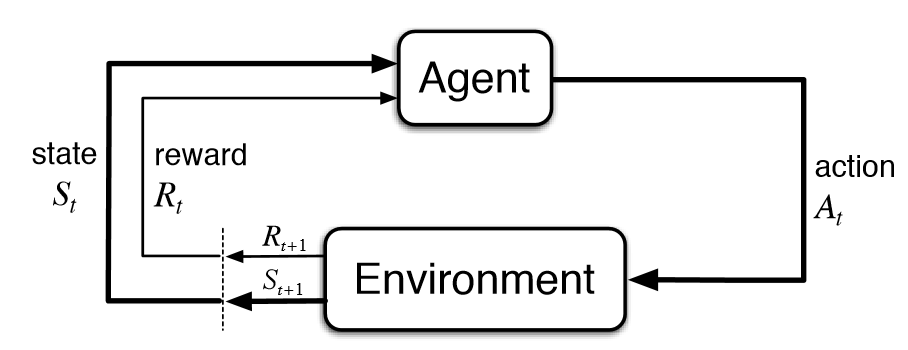
\includegraphics[width=0.7\textwidth]{figs/rl.png}
    \caption{Reinforcement Learning\protect\footnotemark[1]}
    \label{fig:rldiag}
\end{figure}
\footnotetext[1]{
\hyperlink{https://towardsdatascience.com/reinforcement-learning-101-e24b50e1d292}
{https://towardsdatascience.com/reinforcement-learning-101-e24b50e1d292}}

% \begin{quote}
%     Some key terms that describe the basic elements of an RL problem are\footnotemark[1]:
%     \begin{itemize}
%         \item Environment: Physical world in which the agent operates
%         \item State: Current situation of the agent
%         \item Reward: Feedback from the environment
%         \item Policy: Method to map agent’s state to actions
%         \item Value: Future reward that an agent would receive by taking an action in a particular state
%     \end{itemize}
% \end{quote}

Compared with supervised learning, the reward in RL may only be given occasionally and summarily
(e.g. if the agent eventually reaches a desired state after a path of actions)

\subsection{Data}

Common datasets (Benchmark):
\begin{itemize}
    \item small image datasets: MNIST [1,28,28] (extend to EMNIST, fashion-MNIST), CIFAR-10 [3,32,32];
    \item large image datasets: ImageNet [3,256,256];
    \item text datasets for text classification: IMDB movie review dataset;
    \item text datasets for machine translation: documents from multilingual organizations 
    (e.g. Canadian parliament and EU), WMT dataset;
    \item seq2seq tasks (e.g. document summarication and question answering): ?.
\end{itemize}

\textbf{TF-IDF}: term frequency-inverse document frequency.\unsure{
weighted BoW that reduce the importance of uninformative terms
}
TF$_{ij}$ is the frequency of term $i$ in document $j$, and 
IDF$_i\triangleq{\frac{N}{1+\text{DF}_i}}$, 
where $DF_i$ is the number of documents with term $i$.
\begin{gather}
    \text{TF-IDF}_{ij}=\log{\text{TF}_{ij}+1}\times\text{IDF}_i
\end{gather}

\textbf{Word embeddings}: 
\unsure{
Usually self-supervised models were adopted to build a pre-trained word embeddings 
based on large-scale contexts.
}\unsure{
The embeddings with similar meanings be often close in some metric space.}
map sparse and vocabulary-length (high-dimensional) vectors to 
dense and low-dimensional ones (embeddings).

Strategies to deal with OOV:
\begin{enumerate}
    \item replace all novel words with $\mathtt{UNK}$;
    \item byte-pair encoding: finer-grained subword structure embedding;
\end{enumerate}

Let $\bm{M}\in\mathbb{I}^{N\times{D}}$ indicates the missing status of feature $\bm{X}$:
$M_{nd}=1$ if $X_{nd}$ is missing and let $\bm{X}_v~(\bm{M}_v=\bm{0})$ and 
$\bm{X}_h~(\bm{M}_h=\bm{1})$ 
are visible and missing parts of features, respectively. 
The outcome labels $\mathbf{Y}$ are full observed.\unsure{
Missing data handling is a complex topic,
also important in \textit{clinical trial designing}, 
and will be discussed later and further.
}
\begin{itemize}
    \item \textbf{missing completely at random} (MCAR): 
    $p(\bm{M}|\bm{X}_v,\bm{X}_h,\bm{Y})=p(\bm{M})$,
    the missingness does not depend on the hidden/observed features;
    \item \textbf{missing at random} (MAR):
    $p(\bm{M}|\bm{X}_v,\bm{X}_h,\bm{Y})
    =p(\bm{M}|\bm{X}_v,\bm{Y})$,
    the missingness does not depend on the hidden features but may depend on the visible features;
    \item \textbf{not missing at random} (NMAR): otherwise
\end{itemize}

\begin{note}
    In the MCAR/MAR case, the missingness mechanism can be ignored since missingness is
    independent with the unobserved features. 
    And \textbf{this book always makes the MAR assumption}.
\end{note}

\section{Foundations}
\begin{quote}
    \citep{pml1Book} -- Chapter 2-8.
\end{quote}

\subsection{Probability: Univariable and Multivariable Models}

Types of uncertainty:
\begin{enumerate}
    \item \textbf{model uncertainty}: or epistemic uncertainty,
    caused by our ignorance of the underlying hidden causes or mechanism generating the data;
    \item \textbf{data uncertainty}: or aleatoric uncertainty,
    caused by intrinsic variability (the true model generating data randomly).
\end{enumerate}

Paradigm of binary classification with the assumption of probability output:
\begin{gather}
    p(y|\bm{x},\bm{\theta})
    =\text{Bernoulli}(y|\sigma(f(\bm{x};\bm{\theta})))
\end{gather}
where basic property of neuron, activation function $\sigma(a)$, in a network's output layer is compressing the value of unconstrained function to $[0,1]$, 
one example with good characteristics (refer to \citep{pml1Book} Table 2.3) 
of which is the sigmoid function $\frac{1}{1+e^{-a}}$, 
and the variety of $f$'s contributes to the contemporary blossom of deep learning architectures, 
the easiest one of which is linear model $\bm{w}^T\bm{x}+b$. (Logistic regression: Binomial+Sigmoid \& Multinomial+Softmax
\unsure{log-sum-exp trick for computer friendly to avoid floating-point overflow})

Paradigm of regression:
\begin{gather}
    p(y|\bm{x};\bm{\theta})
    =\mathcal{N}(y|
    f_\mu(\bm{x};\bm{\theta}),
    f_\sigma^2(\bm{x};\bm{\theta})
    )
\end{gather}
where $f_\mu\in\mathbb{R}$ predicts the mean 
and $f_\sigma^2\in\mathbb{R}^+$ predicts the variance.
Recall the two types of uncertainty,
the \textbf{uncertainty of data} ($y$) is presented by $f_\sigma(\bm{x};\bm{\hat{\theta}})$ and 
the \textbf{uncertainty of model} ($\bm{\theta}$) is presented by 
$\mathrm{Var}f_\mu(\bm{x};\bm{\theta})$.

Gaussian (or Normal) distribution has good characteristics
\begin{enumerate}
    \item with two parameters $\mu,\sigma^2$, easy to interpret;
    \item by central limit theorem (modeling the noise from multiple sources);
    \item with the least number of assumptions;
    \item with simple form, easy to implement but highly effective.
\end{enumerate}

\textbf{Heavy-tail} distributions, say, 
Student, Cauchy, and Laplace (double sided Exp.) distributions, 
is robust to outliers.\unsure{
Grafting of Normal main body and Cauchy tails are also used to deal with outliers like RCTD.
} 
It is common to set $\nu=4$, if greater, then Student dist. approaches to $\mathcal{N}$.

\textbf{Monte Carlo approximation}. 
Consider an arbitrary transformation $\bm{Y}=g(\bm{X})$,
it is often difficult to compute the induced distribution $f_{\bm{Y}}(\bm{y})$ analytically,
but it can be approached by drawing a large amount of samples 
from the original distribution $f_{\bm{X}}(\bm{x})$:
\begin{gather}
    f_{\hat{\bm{Y}}}(\bm{y})
    \triangleq
    \frac{1}{N}\sum_{s=1}^N\delta(\bm{y}-g(\bm{x}_s))
\end{gather}



% \begin{framed}{\Large

% TODO list in the following week
% \begin{itemize}
%     \item Finish reading the remaining chapters in the Foundation part
%     \item Finish reading \citep{shao2003mathematical} and 
%     do the exercises (for STAT5005)
%     \item Finish organizing the hand writing notes of STAT5010.
% \end{itemize}

% }\end{framed}
\textbf{Simpson's paradox} says that a statistical trend or relationship 
that appears in several difficult groups of data can disappear or reverse sign 
when these groups are combined.

\textbf{Convariance} of multiple r.v.. $\bm{X}=(X_1,\cdots,X_D)$ is defined as\unsure{
Useful in Multivariate Analysis and Linear Model
} 
\begin{align}
    \bm{\Sigma}\triangleq\mathrm{Cov}\bm{X}
    =& \mathbb{E}\left[
    (\bm{X}-\mathbb{E}\bm{X})
    (\bm{X}-\mathbb{E}\bm{X})^T
    \right]\\
    =& \mathbb{E}[\bm{XX}^T]-[\mathbb{E}\bm{X}][\mathbb{E}\bm{X}]^T
\end{align}
\begin{enumerate}
    \item $\mathbb{E}[\bm{XX}^T]=\bm{\Sigma}+\bm{\mu}\bm{\mu}^T$
    \item $\mathrm{Cov}[\bm{AX}+\bm{b}]=\bm{A}\mathrm{Cov}\bm{X}\bm{A}^T$
    \item \improvement{There are some other properties of multiple r.v. waiting to be added.}
\end{enumerate}

\textbf{Multivariate Gaussian/normal} (MVN) r.v. 
$\bm{X}\sim\mathcal{N}(\bm{\mu},\bm{\Sigma})$
\begin{gather}
    f_{\bm{X}}(\bm{x})
    = \frac{1}{(2\pi)^\frac{D}{2}|\bm{\Sigma}|^\frac{1}{2}}
    \exp\left\{ 
        -\frac{1}{2}
        (\bm{x}-\bm{\mu})^T
        \bm{\Sigma}^{-1}
        (\bm{x}-\bm{\mu}) 
    \right\}
\end{gather}

\textbf{Mahalanobis distance} $\Delta$ between $\bm{x}$ and $\bm{\mu}$
under the assumption of above MVN is defined as
\begin{gather}
    \Delta^2\triangleq
    (\bm{x}-\bm{\mu})^T
    \bm{\Sigma}^{-1}
    (\bm{x}-\bm{\mu}),
\end{gather}
implying that \uline{the points with a same density have a same Mahalanobis distance 
away from the population mean point $\bm{\mu}$}, say, like contours.
It can be interpreted as Euclidean distance in a new coordinate 
from the original coordinate by the transformation of 
$\bm{\Sigma}^{-1}$,
which can be computed by eigendecomposition:
\begin{gather}
    \bm{\Sigma}
    = \sum_{d=1}^D{\lambda_d\bm{u}_d\bm{u}_d^T}
    % = \bm{U}\mathrm{diag}(\lambda_1,\cdots,\lambda_D)\bm{U}^T\\
    = \bm{U}\bm{D}\bm{U}^T\\
    \bm{\Sigma}^{-1}
    = \sum_{d=1}^D{\lambda_d^{-1}\bm{u}_d\bm{u}_d^T}
    % = \bm{U}\mathrm{diag}(\lambda_1,\cdots,\lambda_D)^{-1}\bm{U}^T
    = \bm{U}\bm{D}^{-1}\bm{U}^T
    \triangleq \bm{\Lambda}
\end{gather}
where $\bm{U}=[\bm{u}_1,\cdots,\bm{u}_D]$ is eigenvectors for rotation and 
$\bm{D}=\mathrm{diag}(\lambda_1,\cdots,\lambda_D)$ is eigenvalues for scaling.\unsure{
This procedure is similar with the standardization of univariable Gaussian.}


\textbf{Marginals and conditionals of an MVN}: \info{
Marginals and conditionals of a multi-variable model is important and frequently used conclusion.
}
Suppose $\bm{X}=[\bm{X}_1,\bm{X}_2]^T\sim\mathcal{N}(\bm{\mu},\bm{\Sigma})$, where
\begin{gather}
    \bm{\mu}=\left[\begin{array}{c}
        \bm{\mu}_1 \\
        \bm{\mu}_2
    \end{array}\right],~
    \bm{\Sigma}=\left[\begin{array}{cc}
        \bm{\Sigma}_{11} & \bm{\Sigma}_{12} \\
        \bm{\Sigma}_{21} & \bm{\Sigma}_{22}
    \end{array}\right],~\text{and}~
    \bm{\Lambda}
    =\bm{\Sigma}^{-1}=\left[\begin{array}{cc}
        \bm{\Lambda}_{11} & \bm{\Lambda}_{12} \\
        \bm{\Lambda}_{21} & \bm{\Lambda}_{22}
    \end{array}\right]
\end{gather}
is the \textbf{precision matrix}.
$\Rightarrow$
\begin{align}
    \bm{X}_1
    \sim& \mathcal{N}(\bm{\mu}_1,\bm{\Sigma}_{11}),\\
    \bm{X}_1|\bm{X}_2
    \sim& \mathcal{N}
    (\bm{\mu}_{1|2},\bm{\Sigma}_{1|2})
\end{align}
where 
\begin{align}
    \bm{\mu}_{1|2}
    =& \bm{\Sigma}_{1|2}
    [\bm{\Lambda}_{11}\bm{\mu}_1
    -\bm{\Lambda}_{12}(\bm{X}_2-\bm{\mu}_2)],\\
    \bm{\Sigma}_{1|2}
    =& \bm{\Sigma}_{11}
    -\bm{\Sigma}_{12}\bm{\Sigma}_{22}^{-1}\bm{\Sigma}_{21}
    =\bm{\Lambda}_{11}^{-1}.
\end{align}

% \begin{example}
%     $~$\\
%     $\bm{\Sigma}=\left[\begin{array}{cc}
%         \sigma_1^2 & \rho\sigma_1\sigma_2 \\
%         \rho\sigma_1\sigma_2 & \sigma_2^2
%     \end{array}\right]$, and compute the marginal and conditional distribution.
% \end{example}

\begin{example}
    \textbf{Missing value imputation}\\
    infer the missing entries 
    by exploiting the correlation (in $\bm{\Sigma}$) amongst the dimensions,
    say, computing 
    $p(\bm{x}_{n,\bm{h}}|\bm{x}_{n,\bm{v}},\bm{\theta})$
    and obtain the posterior mean (optimally guessed values) and variance (confidence measure).
\end{example}


\textbf{Linear Gaussian system}.
Let $\bm{Z}\in\mathbb{R}^L$ be an unknown vector of values, 
and $\bm{Y}\in\mathbb{R}^D$ be some \textbf{noisy measurement} of $\bm{Z}$:
\begin{align}
    \bm{Z}
    \sim& \mathcal{N}(\bm{\mu}_z,\bm{\Sigma}_z)\\
    \bm{Y}|\bm{Z}=\bm{z}
    \sim& \mathcal{N}(\bm{Wz}+\bm{b},\bm{\Sigma}_y)
\end{align}
The joint distribution of $[\bm{Z},\bm{Y}]$ follows is Gaussain 
$\mathcal{N}(\bm{\mu},\bm{\Sigma})$, where\unsure{
The unconditional variance of $\bm{Y}$ includes its conditional variance, $\bm{\Sigma}_y$,
and the squared weight-scaled variance of $\bm{Z}$, $\bm{W\Sigma}_z\bm{W}^T$.
}
\begin{gather}
    \bm{\mu}
    = \left[\begin{array}{c}
        \bm{\mu}_z \\
        \bm{W\mu}_z+\bm{b} 
    \end{array}\right],~
    \bm{\Sigma}
    = \left[\begin{array}{cc}
        \bm{\Sigma}_z & \bm{\Sigma}_z\bm{W}^T \\
        \bm{W\Sigma}_z & \bm{\Sigma}_y+\bm{W\Sigma}_z\bm{W}^T
    \end{array}\right]
\end{gather}

\begin{example}
    \textbf{relationship from observations to latent factors}\\
    Infer the \uline{relationship from observations to latent factors}: $\bm{Y}\to\bm{Z}$ by Bayes rule:
    \begin{align}
        \bm{Y}
        \sim& \mathcal{N}(\bm{W\mu}_z+\bm{b},\bm{\Sigma}_y+\bm{W\Sigma}_z\bm{W}^T)\\
        \bm{Z}|\bm{Y}=\bm{y}
        \sim& \mathcal{N}(\bm{\mu}_{z|y},\bm{\Sigma}_{z|y}),
    \end{align}
    where
    \begin{align}
        \bm{\mu}_{z|y}
        =& \bm{\Sigma}_{z|y}\left[
            \bm{W}^T\bm{\Sigma}_y^{-1}(\bm{y}-\bm{b})+\bm{\Sigma}_z^{-1}\bm{\mu}_z
        \right]~\text{and}~\\
        \bm{\Sigma}_{z|y}^{-1}
        =& \bm{\Sigma}_z^{-1}+\bm{W}^T\bm{\Sigma}_y^{-1}\bm{W}
    \end{align}
\end{example}

\begin{example}
    \textbf{shrinkage} and \textbf{Singal-to-noise ratio}\\
    Suppose $Y_i=Z+\varepsilon$ is the observed signal with 
    $\varepsilon\sim\mathcal{N}(0,\Sigma_y)$ and
    $Y_i|Z=z\sim\mathcal{N}(z,\Sigma_y)$,
    and $z\sim\mathcal{N}(\mu_0,\Sigma_0)$ is the true signal, 
    then $Z|\bm{y}\sim\mathcal{N}(\mu_N,\Sigma_N)$, where
    \begin{align}
        \Sigma_N
        =& \left(\Sigma_0^{-1}+N\Sigma_N^{-1}\right)^{-1}\\
        \mu_N
        % =& \frac{\Sigma_y/N}{\Sigma_0+\Sigma_y/N}\mu_0+\frac{\Sigma_0}{\Sigma_0+\Sigma_y/N}\Bar{y}_N\\
        % =& \mu_0 + ({\Bar{y}_N-\mu_0})\frac{\Sigma_0}{\Sigma_y/N+\Sigma_0}\\
        =& \Bar{y}_N - (\Bar{y}_N-\mu_0)\frac{\Sigma_y/N}{\Sigma_y/N+\Sigma_0} \label{eq:shrinkage}
    \end{align}
    The data is adjusted towards the prior mean with the increasing of noise deviation, called \textbf{shrinkage}, by Equation (\ref{eq:shrinkage}).
    And the amount of shrinkage is defined as \textbf{signal-to-noise ratio}, 
    \begin{gather}
        \text{SNR}\triangleq\frac{\mathbb{E}Z^2}{\mathbb{E}\varepsilon^2}=\frac{\Sigma_0+\mu_0^2}{\Sigma_y}
    \end{gather}
    By increasing the number of observations, 
    the SNR can be amplified through reducing the variance of noise $\varepsilon$, 
    and this conclusion can be extend to multi-variable case.
\end{example}
% \unsure{
%     recall the convex combination of the prior and the data
%     }
\begin{example}
    \textbf{Senser fusion}\\
    There are $M$ sensors (measurement devices) and $N_m$ observations for each devices, 
    the the signals $Y_{1,m},\cdots,Y_{n,m},\cdots,Y_{N_m,m}|\bm{Z}=\bm{z}\overset{iid}{\sim}\mathcal{N}(\bm{z},\Sigma_m)$. Sensor fusion is to combine the evidence together, to compute $p(\bm{z}|\bm{y})$.
\end{example}

\begin{question}
    Why is exponential family so important?
\end{question}

\textbf{Maximum entropy derivation of the exponential family}:
Recall \textbf{KL divergence} of two distributions, $p$ and $q$, not symmetric
\begin{gather}
    \infdiv{p}{q}
    \triangleq\left\{
    \begin{array}{ll}
        \int_\mathcal{X}{p(x)\log\frac{q(x)}{p(x)}}dx & X~\text{continuous} \\
        \sum_x{p(x)\log\frac{p(x)}{q(x)}} & X~\text{discrete}
    \end{array}\right.
\end{gather}
To find a distribution $p$ that minimizes the $\infdiv{p}{q}$ with a given priori $q$
with moments constraints of observed data
\begin{gather}
    p^*=\argmin_p\infdiv{p}{q}\\
    \mathrm{s.t.}~\sum_x{p(x)}=1
    ~\text{and}~
    \sum_x{p(x)f_k(x)}=F_k,~k=1,\cdots,K
\end{gather}
The Lagrangian is given by
{\small\begin{gather}
    J(p,\bm{\lambda})
    =- \sum_x{p(x)\log\frac{p(x)}{q(x)}}
    + \lambda_0\left[1-\sum_x{p(x)}\right]
    + \sum_k{\lambda_k\left[ F_k-\sum_x{p(x)f_k(x)} \right]}\\
\Rightarrow
    p^*(x)=\frac{1}{Z}q(x)\exp\left\{-\sum_k{\lambda_kf_k(x)}\right\}
\end{gather}}
which is exactly the form of exponential family and where $Z$ is the normalization term.
e.g. if $f_1(x)=x$ and $f_2(x)=x^2$, then the best distribution with minimum KL divergence 
(or maximum entropy) and matching the observed first and second moments is Gaussian distribution.

\textbf{Gaussain mixture model} (GMM) or \textbf{mixture of Gaussian} (MoG): 
the probability of each data point $\bm{y}_n$\unsure{
Are the proportion $\pi_k$'s different for each data points?
What is the relationship between $r_{nk}$ and $\pi_k$ in Equation (\ref{eq:mogpir})?
} is determined 
by certain weights of multiple distinct Gaussian models,
often used for clustering, e.g. K-means with $\bm{\Sigma}_k=\bm{I}$, $k=1,\cdots,K$.
\begin{gather}
    p(\bm{y}|\bm{\theta})=\sum_{k=1}^K{\pi_k\mathcal{N}(\bm{\mu}_k,\bm{\Sigma}_k)}
\end{gather}
\begin{align}
    \hat{\bm{\theta}}
    =& \argmax_{\bm{\theta}}\log{p(\bm{y}_1,\cdots,\bm{y}_N|\bm{\theta})}~\text{(by MLE)}\\
    \hat{\pi}_{nk}
    \overset{?}{=}& r_{nk}\triangleq p(z_n=k|\bm{y}_n,\hat{\bm{\theta}}) \label{eq:mogpir}\\
    =& \frac{p(z_n=k|\hat{\bm{\theta}})p(\bm{y}_n|z_n=k,\hat{\bm{\theta})z}}
    {\sum_{k'=1}^K{p(z_n=k'|\hat{\bm{\theta}})p(\bm{y}_n|z_n=k',\hat{\bm{\theta})}}}~\text{(by Bayes)}
\end{align}
\improvement{
The optimization process of EM or SGD will be discussed in \citep{pml1Book}, Chapter 8.
}

\textbf{Bernoulli mixture model} (BMM) or \textbf{mixture of Bernoullis} (MoB):
similar with MoG:
\begin{gather}
    p(\bm{y}|\bm{\theta})=\sum_{k=1}^K{\pi_k\underbrace{\prod_{d=1}^D\mathrm{Ber}(y_d|\mu_{dk})}_{\text{proba. of r. vec.}}}
\end{gather}

\textbf{Ordered Markov property} in a \textbf{Bayesian network} is that 
each node $Y_i$ is conditionally independent of all its predecessors ($\bm{Y}_{\text{pre}(i)}$) given its parents ($\bm{Y}_{\text{par}(i)}$):
\begin{gather}
    Y_i\perp\bm{Y}_{\text{pre}(i)\setminus\text{par}(i)}|\bm{Y}_{\text{par}(i)}\\
    p(\bm{Y}_{1:N_G})=\prod_{i=1}^{N_G}p\left(Y_i|\bm{Y}_{\text{par}(i)}\right)
\end{gather}
where $p\left(Y_i|\bm{Y}_{\text{par}(i)}\right)$ is called \textbf{conditional probability distribution} (CPD), 
which can be written as the conditional probability table (CPT) 
when the status of each node is (discrete) categorical distribution.
In Markov chain model, 
$p(y_t|y_{t-1})$ is called \textbf{transition function/kernel} (or \textbf{state transition matrix} in the case of discrete status) and is \textbf{stationary/time-invariant} under the assumption that $p(y_t|y_{t-1})$ is the same for all time steps.

\begin{figure}[hptb]
    \centering
    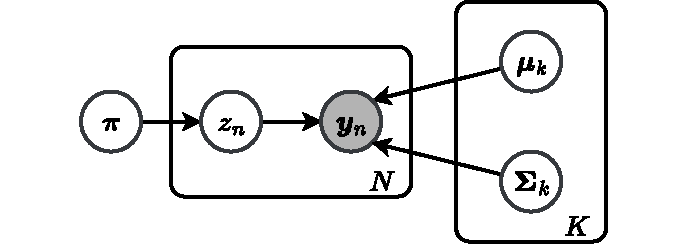
\includegraphics[width=0.5\textwidth]{figs/mixgaussian.pdf}
    \caption{A Gaussian mixture model represented as a graphical model}
    \label{fig:maxgaussian}
\end{figure}

\begin{example}
    \textbf{GMM represented as a graphical model}\\
    Viewing all variables, including model's parameters and obverations, 
    follow a generative story like Figure (\ref{fig:maxgaussian})
    {\small\begin{gather}
        p(\bm{y}_{1:N},\bm{z}_{1:N},\bm{\theta})
        = p(\bm{pi})
        \left[ \prod_{k=1}^K p(\bm{\mu}_k)p(\bm{\Sigma}_k) \right]
        \left[ \prod_{n=1}^N p(z_n|\bm{\pi})p(\bm{y}_n|z_n,\bm{\mu}_{1:K},\bm{\Sigma}_{1:K}) \right]
    \end{gather}}
    where latent variable $z_n\sim\text{Cat}(\bm{\pi})$ and model's parameters
    $\bm{\theta}=(\bm{\pi},\bm{\mu}_{1:K},\bm{\Sigma}_{1:K})$ are all unknown.
\end{example}



% \begin{framed}{\large
% TODO list in the following week
% \begin{itemize}
%     \item Finish reading the remaining chapters in the Foundation part
%     \item Finish reading \citep{shao2003mathematical} and 
%     do the exercises (for STAT5005)
%     \item Finish organizing the hand writing notes of STAT5010.
% \end{itemize}
% }\end{framed}




% ############################### WK 2 #######################################

% \setcounter{section}{2}
% \setcounter{subsection}{2}
% \begin{center}
% \textit{Continue Chapter 2 \& 3 univariate and multivariate models}
% \end{center}

% \subsection{Statistics}

\begin{question}
    Why can MLE be used so uniformly?
\end{question}

\textbf{Maximum likelihood estimation} (MLE) and \textbf{maximum a posterior estimation} (MAP):
$\hat{\bm{\theta}}_{MLE}$ -- the parameters' estimation that assign the highest probability to the observations;
$\hat{\bm{\theta}_{MAP}}$ -- the parameters' estimation maximizing the posterior probability under some priori $\pi(\bm{\theta})$. 
If \uline{the priori is a uniform distribution}, 
then $\hat{\bm{\theta}}_{MLE}=\hat{\bm{\theta}}_{MAP}$.\unsure{
Reason 1
}
\begin{gather}
    \hat{\bm{\theta}}_{MLE}
    \triangleq \argmax_{\bm{\theta}}p(\mathcal{D}|\bm{\theta})\\
    \hat{\bm{\theta}}_{MAP}
    \triangleq \argmax_{\bm{\theta}}p(\bm{\theta}|\mathcal{D})
    = \argmax_{\bm{\theta}}p(\mathcal{D}|\bm{\theta})\pi(\bm{\theta})
\end{gather}
\textbf{Kullback Leibler divergence} (KL divergence): 
A standard way to measure the dissimilarity between probability distribution $p$ and $q$.
\begin{align}
    \infdiv{p}{q}
    =& \sum_{\bm{y}}{p(\bm{y})\log\frac{p(\bm{y})}{q(\bm{y})}}\\
    =& \underbrace{\sum_{\bm{y}}{p(\bm{y})\log p(\bm{y})}}_{-\mathbb{H}(p)\text{:entropy}}
    - \underbrace{\sum_{\bm{y}}{p(\bm{y})\log q(\bm{y})}}_{-\mathbb{H}_{\text{CE}}(p,q)\text{:cross-entropy}}
\end{align}
If \uline{$q(\bm{y})=p(\bm{y}|\bm{\theta})$ and $p(\bm{y})=p_\mathcal{D}(\bm{y})$}, 
then $\infdiv{p}{q}=\text{const}+\mathrm{NNL}(\bm{\theta})$.\unsure{Reason 2}
which shows the relationship between MLE and KL divergence.
And above all justify usage of MLE from the perspectives of Bayesain and empirical distribution.

\begin{example}
    \textbf{MLE for linear regression} aka\\
    \textbf{ordinary least squares} or OLS estimate
    \begin{align}
        p(y|\bm{x};\bm{\theta})
        =& \mathcal{N}(\bm{w}^T\bm{x},\sigma^2)\\
        \hat{\bm{w}}_{OLS}\equiv\hat{\bm{w}}_{MLE}
        \triangleq& \argmin_{\bm{w}}\text{NLL or RSS or MSE or RMSE}\\
        =& (\bm{X}^T\bm{X})^{-1}\bm{X}^T\bm{y}
    \end{align}
\end{example}

\textbf{Empirical risk minimization} (ERM) 
\begin{gather}
    \mathcal{L}(\bm{\theta})=\frac{1}{N}\sum_{n=1}^N\ell(\bm{y}_n,\bm{\theta};\bm{x}_n)
\end{gather}
where $\ell(\cdot)$ is any loss function that measures the mismatchness with expected outcomes, 
(if $\ell(\bm{y}_n,\bm{\theta};\bm{x}_n)=-\log{p(\bm{y}_n|\bm{\theta},\bm{x}_n)}$,
then $\mathcal{L}(\bm{\theta})=\text{NLL}(\bm{\theta})$ and ERM is MLE).\unsure{Reason 3}
% \textbf{Surrogate loss function}: 
% The surrogate is usually chosen to be a maximally tight
% convex upper bound, which is then easy to minimize, e.g. 

% \begin{enumerate}[(i)]
%     \item 0-1 loss: 
%     $\ell_{01}(\bm{y}_n,\bm{\theta};\bm{x}_n)=\mathbb{I}(\bm{y}_n\neq f(\bm{x}_n;\bm{\theta})$
%     \item :
    
% \end{enumerate}

\begin{figure}[hptb]
    \centering
    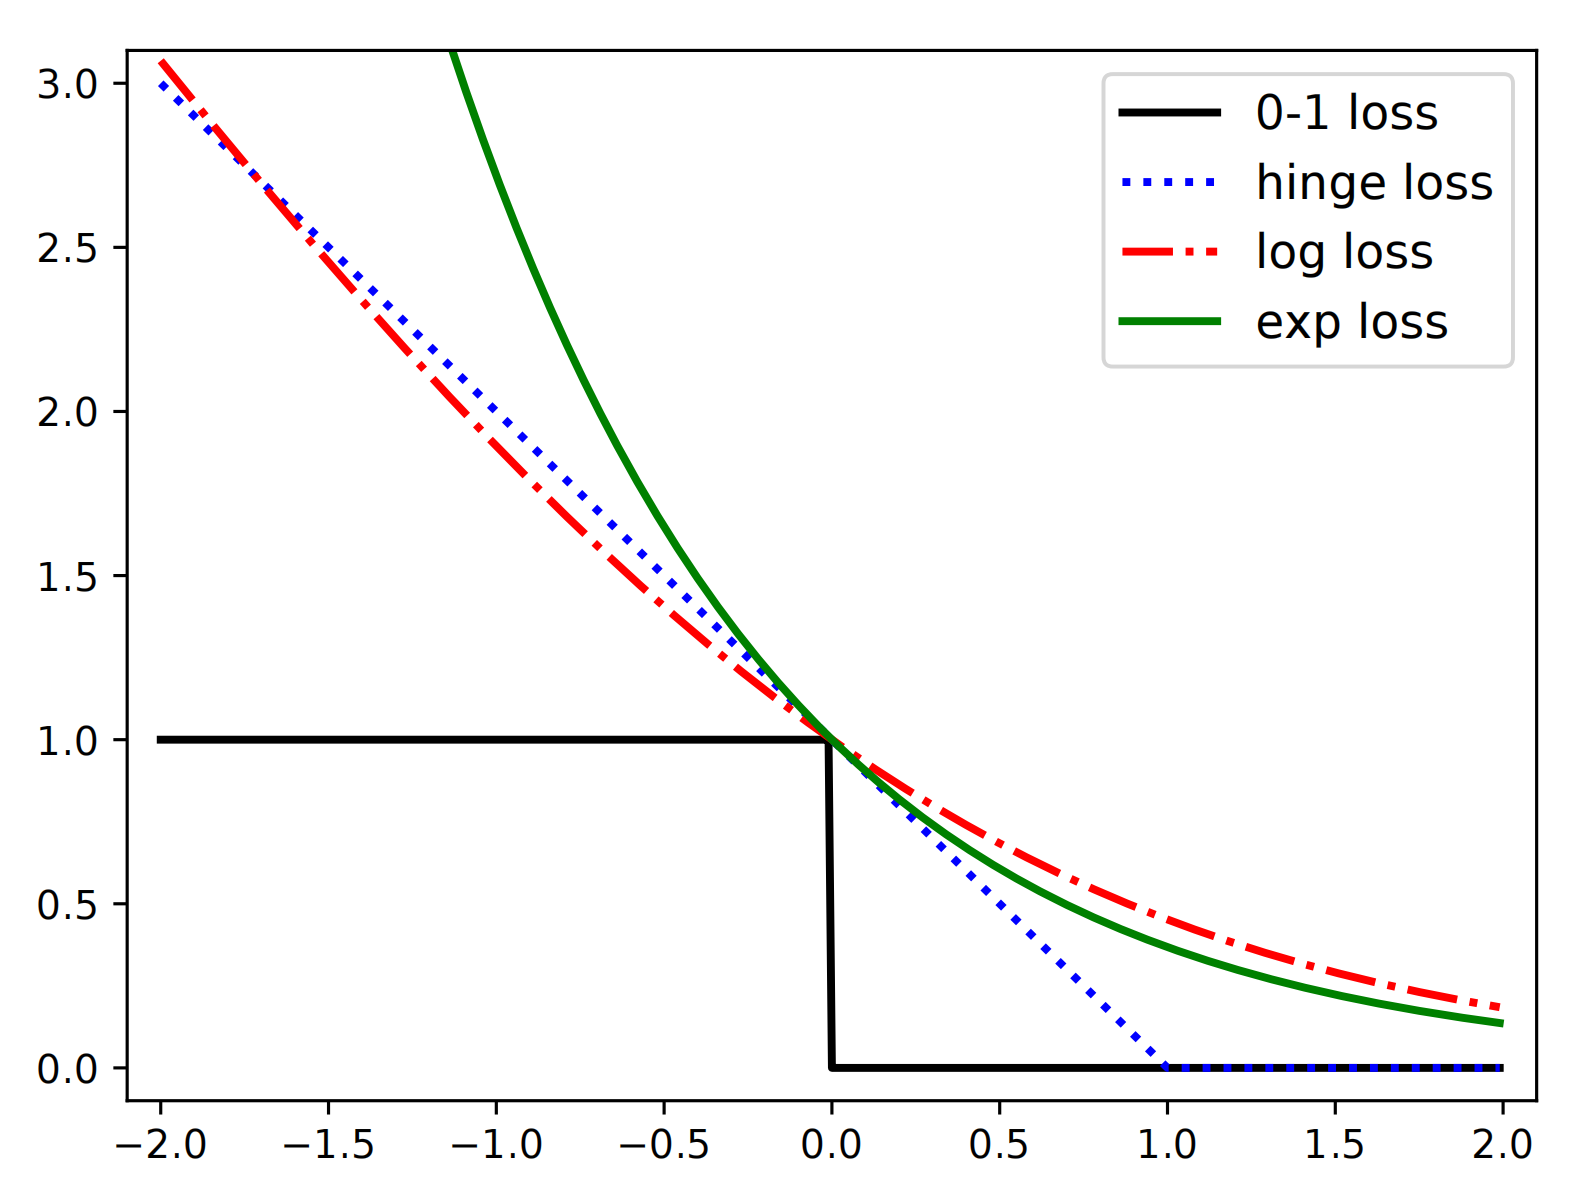
\includegraphics[width=0.5\textwidth]{figs/lossfunc.png}
    \caption{Loss functions for \uline{binary classifiers}}
    {\footnotesize Horizontal axis: $z=yf(\bm{x};\bm{\theta})$. \\
    0-1 loss: $\mathbb{I}(z<0)$;
    Hinge loss: $\max\{0,1-z\}$;
    Log-loss: $\log_2{(1+e^{-z})}$;
    Exp-loss: $e^{-z}$.}
    \label{fig:lossfunc}
\end{figure}

\textbf{Estimation method of moments} (MOM): 
equate the \uline{theoretical moments (functions of parameters)},
to the \uline{empirical moments},
where we need the same number of simultaneous equations for solving $K$ unknown parameters,
to avoid difficult computation in MLE 
but with less efficiency of data usage, so can be used to initialize iterative algorithms for MLE.

\textbf{Online (recursive) estimation} with recursive update $f$:
\begin{gather}
    \hat{\bm{\theta}}_t=f(\hat{\bm{\theta}}_{t-1},\bm{y}_t)
\end{gather}

\begin{example}
    \textbf{Exponentially-weighted moving average} (EWMA)
    \begin{align}
        \hat{\bm{\mu}}_t
        =& \beta\hat{\bm{\mu}}_{t-1}+(1-\beta)\hat{\bm{y}}_t\\
        =& \beta^t\bm{y}_0 + (1-\beta)\beta^{t-1}\bm{y}_1 + \cdots + (1-\beta)\beta\bm{y}_{t-1} + (1-\beta)\bm{y}_t
    \end{align}
    where a smaller $\beta$ forgets the past data more quickly and 
    adapts to the more recent data more rapidly.
\end{example}

\textbf{Regularization} term $C(\bm{\theta})$ in the loss function is 
a given measure for the parameters' complexity to avoid overfitting:
\begin{gather}
    \mathcal{L}(\bm{\theta};\lambda)
    = \frac{1}{N}\sum_{n=1}^N\ell(\bm{y}_n,\bm{\theta};\bm{x}_n)
    + \lambda C(\bm{\theta})
\end{gather}
where $C(\bm{\theta})$ can be some $-\log{\pi(\bm{\theta})}$,
then objective become a MAP estimation for a given priori $\pi(\bm{\theta})$ for $\lambda=1$.
e.g. add-one smoothing (or \textbf{Laplace's rule of succession}) in Bernoulli distribution with $\pi\sim\text{Beta}(2,2)$ $p\sim$ and shrinkage estimation for $\Sigma$ in multivariate Gaussian with $\pi\sim$ inverse Wishart. 

\textbf{Bayes model averaging} (BMA): make predictions under the posterior distribution of parameters, which weighted the predictions for all possible parameters (models)
\begin{gather}
    \pi(\bm{\theta}|\mathcal{D})
    = \frac{\pi(\bm{\theta})p(\mathcal{D}|\bm{\theta})}{p(\mathcal{D})}\\
    p(\bm{y}|\bm{x},\mathcal{D})
    = \int{p(\bm{y}|\bm{x};\bm{\theta})\pi(\bm{\theta}|\mathcal{D})}d\bm{\theta}
\end{gather}
where $\bm{x}$ is new observations, $\mathcal{D}$ is training data, and 
$p(\bm{y}|\bm{x},\mathcal{D})$ is the final averaging model.


\textbf{Mixtures of priors} by introducing a latent indicator variable $h$
\begin{gather}
    \pi(\bm{\theta})=\sum_k p(h=k)\pi(\bm{\theta}|h=k)
\end{gather}
$\Rightarrow$
\begin{align}
    \pi(\bm{\theta}|\mathcal{D})
    =& \sum_k{p(h=k|\mathcal{D})p(\bm{\theta}|\mathcal{D},h=k)}\\
    p(h=k|\mathcal{D})
    =& \frac{p(h=k)p(\mathcal{D}|h=k)}{\sum_{k'}{p(h=k')p(\mathcal{D}|h=k')}}
\end{align}
\improvement{
The detailed discussion on 
prior, posterior, predictive, and marginal likelihood of
(1) Beta-Binomial, (2)\textbf{Dirichlet-Multinomial}, and (3) Gaussian-Gaussian
are skipped.
}

\textbf{Other priors} besides conjugate priors
\begin{enumerate}[(1)]\label{kspt:noninfo}
    \item \textbf{noninformative prior} or preferred \textbf{minimally informative prior}: 
    let the data speak for itself, 
    e.g. \textbf{flat prior} $\pi\propto 1$ in Gaussian;
    \item \textbf{hierarchical prior}: the hyperparameters in prior also follow some prior --
    $\bm{\phi}\to\bm{\theta}\to\mathcal{D}$;
    \item \textbf{empirical prior}: the prior's hyperparameters $\bm{\phi}$ directly estimated from data $\mathcal{D}$ as shown below
    \begin{gather}
        \hat{\bm{\phi}}(\mathcal{D})
        = \argmax_{\bm{\phi}}p(\mathcal{D}|\bm{\phi})
        = \argmax_{\bm{\phi}}\int{p(\mathcal{D}|\bm{\theta})p(\bm{\theta}|\bm{\phi})}d\bm{\theta}
    \end{gather}
    which is called \textbf{Empirical Bayes} (EB).
\end{enumerate}

Available inference methods:
\begin{itemize}
    \item MLE:
    \begin{gather}
        \hat{\bm{\theta}}
    =\argmax_{\bm{\theta}}
    p(\mathcal{D}|\bm{\theta})
    \end{gather}
    \item MAP: 
    \begin{gather}
        \hat{\bm{\theta}}
    =\argmax_{\bm{\theta}}
    p(\mathcal{D}|\bm{\theta})p(\bm{\theta}|\bm{\phi})
    \end{gather}
    \item MLE-II (EB):
    \begin{gather}
        \hat{\bm{\phi}}
    =\argmax_{\bm{\phi}}
    \int{p(\mathcal{D}|\bm{\theta})p(\bm{\theta}|\bm{\phi})}d\bm{\theta}
    \end{gather}
    \item MAP-II:
    \begin{gather}
        \hat{\bm{\phi}}
    =\argmax_{\bm{\phi}}
    \int{p(\mathcal{D}|\bm{\theta})p(\bm{\theta}|\bm{\phi})p(\bm{\phi})}d\bm{\theta}
    \end{gather}
    \item Full Bayes:
    \begin{gather}
        p(\bm{\theta},\bm{\phi}|\mathcal{D})
    \propto p(\mathcal{D}|\bm{\theta})p(\bm{\theta}|\bm{\phi})p(\bm{\phi})
    \end{gather}
\end{itemize}

\textbf{Computational issues} in Bayesian ML: 
It is usually \uline{intractable to compute $p(\bm{\theta}|\mathcal{D})$}
given $p(\mathcal{D}|\bm{\theta})$ and $p(\bm{\theta})$.
Therefore, methods of \textbf{approximate posterior inference} are necessary.
\begin{itemize}
    \item \textbf{Grid approximation}:  
    brute-force enumerate finite set in partition the space of possible values $\bm{\theta}$.
    \begin{gather}
        p(\bm{\theta}=\bm{\theta}_k|\mathcal{D})
        \approx \frac{p(\mathcal{D}|\bm{\theta}_k)}{\sum_{k'=1}^K{p(\mathcal{D},\bm{\theta}_{k'})}}
    \end{gather}
    \item \textbf{Quadratic (Laplace) approximation}: 
    approximate the posterior by a multivariable Gaussian.
    $\mathcal{E}(\bm{\theta})=-\log{p(\bm{\theta},\mathcal{D})}$ is an \textbf{energy function}, 
    $\hat{\bm{\theta}}$ is the mode ($\Rightarrow\nabla{\mathcal{E}(\bm{\theta})}|_{\bm{\theta}=\hat{\bm{\theta}}}=\bm{0}$), 
    at which $\mathbf{H}$ is Hessian of $\mathcal{E}$.
    \begin{gather}
        p(\bm{\theta}|\mathcal{D})
        \approx \mathcal{N}(\hat{\bm{\theta}},\mathbf{H}^{-1})
    \end{gather}
    \item \textbf{Variational approximation}: 
    find a $q$ minimizing \uline{some discrepancy $D$}, say KL divergence, with target posterior
    in tractable family of distribution $\mathcal{Q}$,
    \begin{gather}
        p(\bm{\theta}|\mathcal{D})
        \approx q^*=\argmin_{q\in\mathcal{Q}} \infdiv{q}{p}
    \end{gather}
    \item \textbf{Monte Carlo approximation}: 
    build an empirical distribution of $\bm{\theta}$ by
    \uline{efficiently create a postrior sample of parameters} $\{\Tilde{\bm{\theta}}_s\}_{s=1}^S\sim p(\bm{\theta}|\mathcal{D})$, 
    without having to evaluate the normalization constant $p(\mathcal{D})$, then
    \begin{gather}
        p(\bm{\theta}|\mathcal{D})
        \approx\frac{1}{S}\sum_{s=1}^S\delta(\bm{\theta}-\Tilde{\bm{\theta}}_s)
    \end{gather}
\end{itemize}

\textbf{Uncertainty represented by \textit{frequentist}}:
$\hat{\bm{\theta}}=\pi(\mathcal{D})$ the estimator's distribution,
\textbf{sampling distribution},
depends on the random data and it is also a r.v..\unsure{
This idea is the same with what we have learnt in STAT5010 for all estimator, 
function of observations, of some transformation of true parameter $g(\bm{\theta})$.
}
However, in the view of frequentist, 
there exists a true single value $\bm{\theta}^*$ that generates the data $\mathcal{D}\sim p(\bm{x}|\bm{\theta}^*)$.
We can find the distribution of $\hat{\bm{\theta}}$, 
$p(\pi(\mathcal{D})=\bm{\theta}|\mathcal{D}\sim\bm{\theta}^*)$ analytically if it is tractable.
If the transformation is intractable, computational issues occur, like in Bayes ML above, and 
then approximation methods are also needed.
\begin{itemize}
    \item \textbf{Gaussian approximation}: \info{
    Gaussian approximation is applied in C-SIDE to model the uncertainty of $\hat{\bm{\beta}}$ for testing $H_0:\bm{\beta}^*=0$}
    by the asymptotic normality of CLT (Theorem \ref{thm:asymnorm}), the distribution of MLE converges to Gaussain
    \begin{gather}
        p(\pi(\mathcal{D})=\bm{\theta}|\mathcal{D}\sim\bm{\theta}^*)
        \to
        \mathcal{N}(\bm{\theta}^*,1/N\mathbf{I}(\bm{\theta}^*))
    \end{gather}
    \item \textbf{(Non-parametric) bootstrap approximation}: a kind of MC technique,
    the distribution of $\hat{\bm{\theta}}$ is approximated 
    by the \uline{empirical distribution from observed data}:
    \begin{gather}
        p(\pi(\mathcal{D})=\bm{\theta}|\mathcal{D}\sim\bm{\theta}^*)
        \approx \frac{1}{S}\sum_{s=1}^S\delta(\bm{\theta}-\pi(\Tilde{\mathcal{D}}_s))
    \end{gather}
    The key of bootstrap is to sample $S$ new datasets $\{\Tilde{\mathcal{D}}_s\}$ with the same size with and from the original dataset,
    $\Tilde{\mathcal{D}}$, with replacement.
    $N:=|\Tilde{\mathcal{D}}|=|\Tilde{\mathcal{D}}_s|$,
    the probability an item is picked at least once is 
    $1-\left(1-\frac{1}{N}\right)^N\to1-e^{-1}$.\unsure{
    Relationship sampling distribution and posterior distribution:
    recall the minimally informative prior in $\S$ \ref{kspt:noninfo}. 
    Sampling distribution only relies on the data.
    }
\end{itemize}


\begin{theorem}\label{thm:asymnorm}
    \textbf{Asymptotic normality}\footnote{
    \citep{pml1Book} Thm 4.7.1
    }\\
    If the parameters are identifiable, then
    \begin{gather}
        p(\pi(\mathcal{D})=\bm{\theta}|\mathcal{D}\sim\bm{\theta}^*)
        \to
        \mathcal{N}(\bm{\theta}^*,1/N\mathbf{I}(\bm{\theta}^*))
    \end{gather}
    where $\mathbf{I}(\bm{\theta}^*)$ is the \textbf{Fisher information matrix} defined as
    \begin{gather}
        \mathbf{I}(\bm{\theta})
        \triangleq\mathbb{E}_{\bm{X}|\bm{\theta}}\left[ 
            (\nabla_{\bm{\theta}}\log{p(\bm{X}|\bm{\theta})})
            (\nabla_{\bm{\theta}}\log{p(\bm{X}|\bm{\theta})})^T
        \right]
    \end{gather}
\end{theorem}

\begin{theorem}
    \textbf{Log-likelihood with twice differentiability}\footnote{
    \citep{pml1Book} Thm 4.7.2
    }\\
    If $\log p(\bm{X}|\bm{\theta})$ is twice differentiable, and under certain regularity conditions,
    \begin{gather}
        \mathbf{I}(\bm{\theta})
        =-\mathbb{E}_{\bm{X}|\bm{\theta}}\left[ 
            (\nabla_{\bm{\theta}}^2\log{p(\bm{X}|\bm{\theta})})
        \right]
    \end{gather}
    which is \uline{Hessian of NLL}.
    \uline{A log-likelihood function with high curvature (large Hessian) will result in
    a low variance estimate, since the parameters are ``well determined'' by the data,
    and hence robust to repeated sampling.}
\end{theorem}\unsure{
Good intuitive understanding. This theorem is also introduced in STAT5010.
}



\textbf{Difference between \uline{credible interval} and \uline{confidence interval}}:
Credible interval: $\mathcal{D}$ fixed (since observed), $\theta$ random;
confidence interval: $\mathcal{D}$ random, $\theta^*$ fixed.
Confidence interval $I(\Tilde{\mathcal{D}})$ such that $P(\theta^*\in I(\Tilde{\mathcal{D}})|\Tilde{\mathcal{D}}\sim\theta^*)=0.95$ \textbf{\textit{does not}} mean that
the true parameter $\theta^*$ is 95\% likely to live inside $I(\Tilde{\mathcal{D}})$, 
which, however, is exactly the quantity given by credible interval {\color{red}$P(\theta\in I|\mathcal{D})$???}.
Confidence interval will cover the true parameter $100(1-\alpha)\%$ of the time.\unsure{
very confusing concept that I still do not understand...
}

% \begin{example}
%     \mathcal{D}=(y_1,y_2) from 
%     \begin{gather}
%         p(y|\theta)=\begin{array}{ll}
%             0.5 & \text{if}~y=\theta \\
%             0.5 & \text{if}~y=\theta+1 \\
%             0 & \text{otherwise}
%         \end{array}
%     \end{gather}
%     If $\theta=39$ and we will obtain the each of data, 
%     $\{(39,39),(39,40),(40,39),(40,40)\}$, 
%     with proba. 0.25
    
% \end{example}

% \textbf{Bias-variance trade-off}


% \textbf{Confidence interval}: uncertainty of a parameter estimate.
% It is worth noting that $p(\pi(\mathcal{D})=\bm{\theta}|\mathcal{D}\sim\bm{\theta}^*)$ 
% is not distribution of true $\bm{\theta}^*$ (with not uncertainty)
% but a guess (r.v.) from data with certain change covering the unknown true $\bm{\theta}^*$.
% \textbf{$100(1-\alpha)\%$ confidence interval} is \uline{any} interval\unsure{
% recall credable region
% }

% \subsection{Decision Theory}

% \subsection{Information Theory}

\subsection{Linear Algebra}

% \subsection{Optimization}
% \begin{framed}{\large
% The schedule last week was over estimated, 
% and a half of tasks are not finished yet.

% TODO list in the following week
% \begin{itemize}
%     \item Finish reading Chapters 7 Linear Algebra and 8 Optimization;
%     \item Finish reading \citep{shao2003mathematical} Chapter 1 and 
%     do the exercises (for STAT5005).
% \end{itemize}
% }
% \end{framed}








% ############################### WK 4 #######################################
% \setcounter{section}{2}
% \setcounter{subsection}{4}
% \begin{center}
% \textit{
% Continue read Chapter 8 from $\S$ 8.6, \\
% and Chapters 5 and 6 (Decision Theory $\And$ Information Theory)\\
% But, the organization of typing notes is still under going...}
% \end{center}



% \subsection{Decision Theory}
% \begin{figure}[htpb]
%     \centering
%     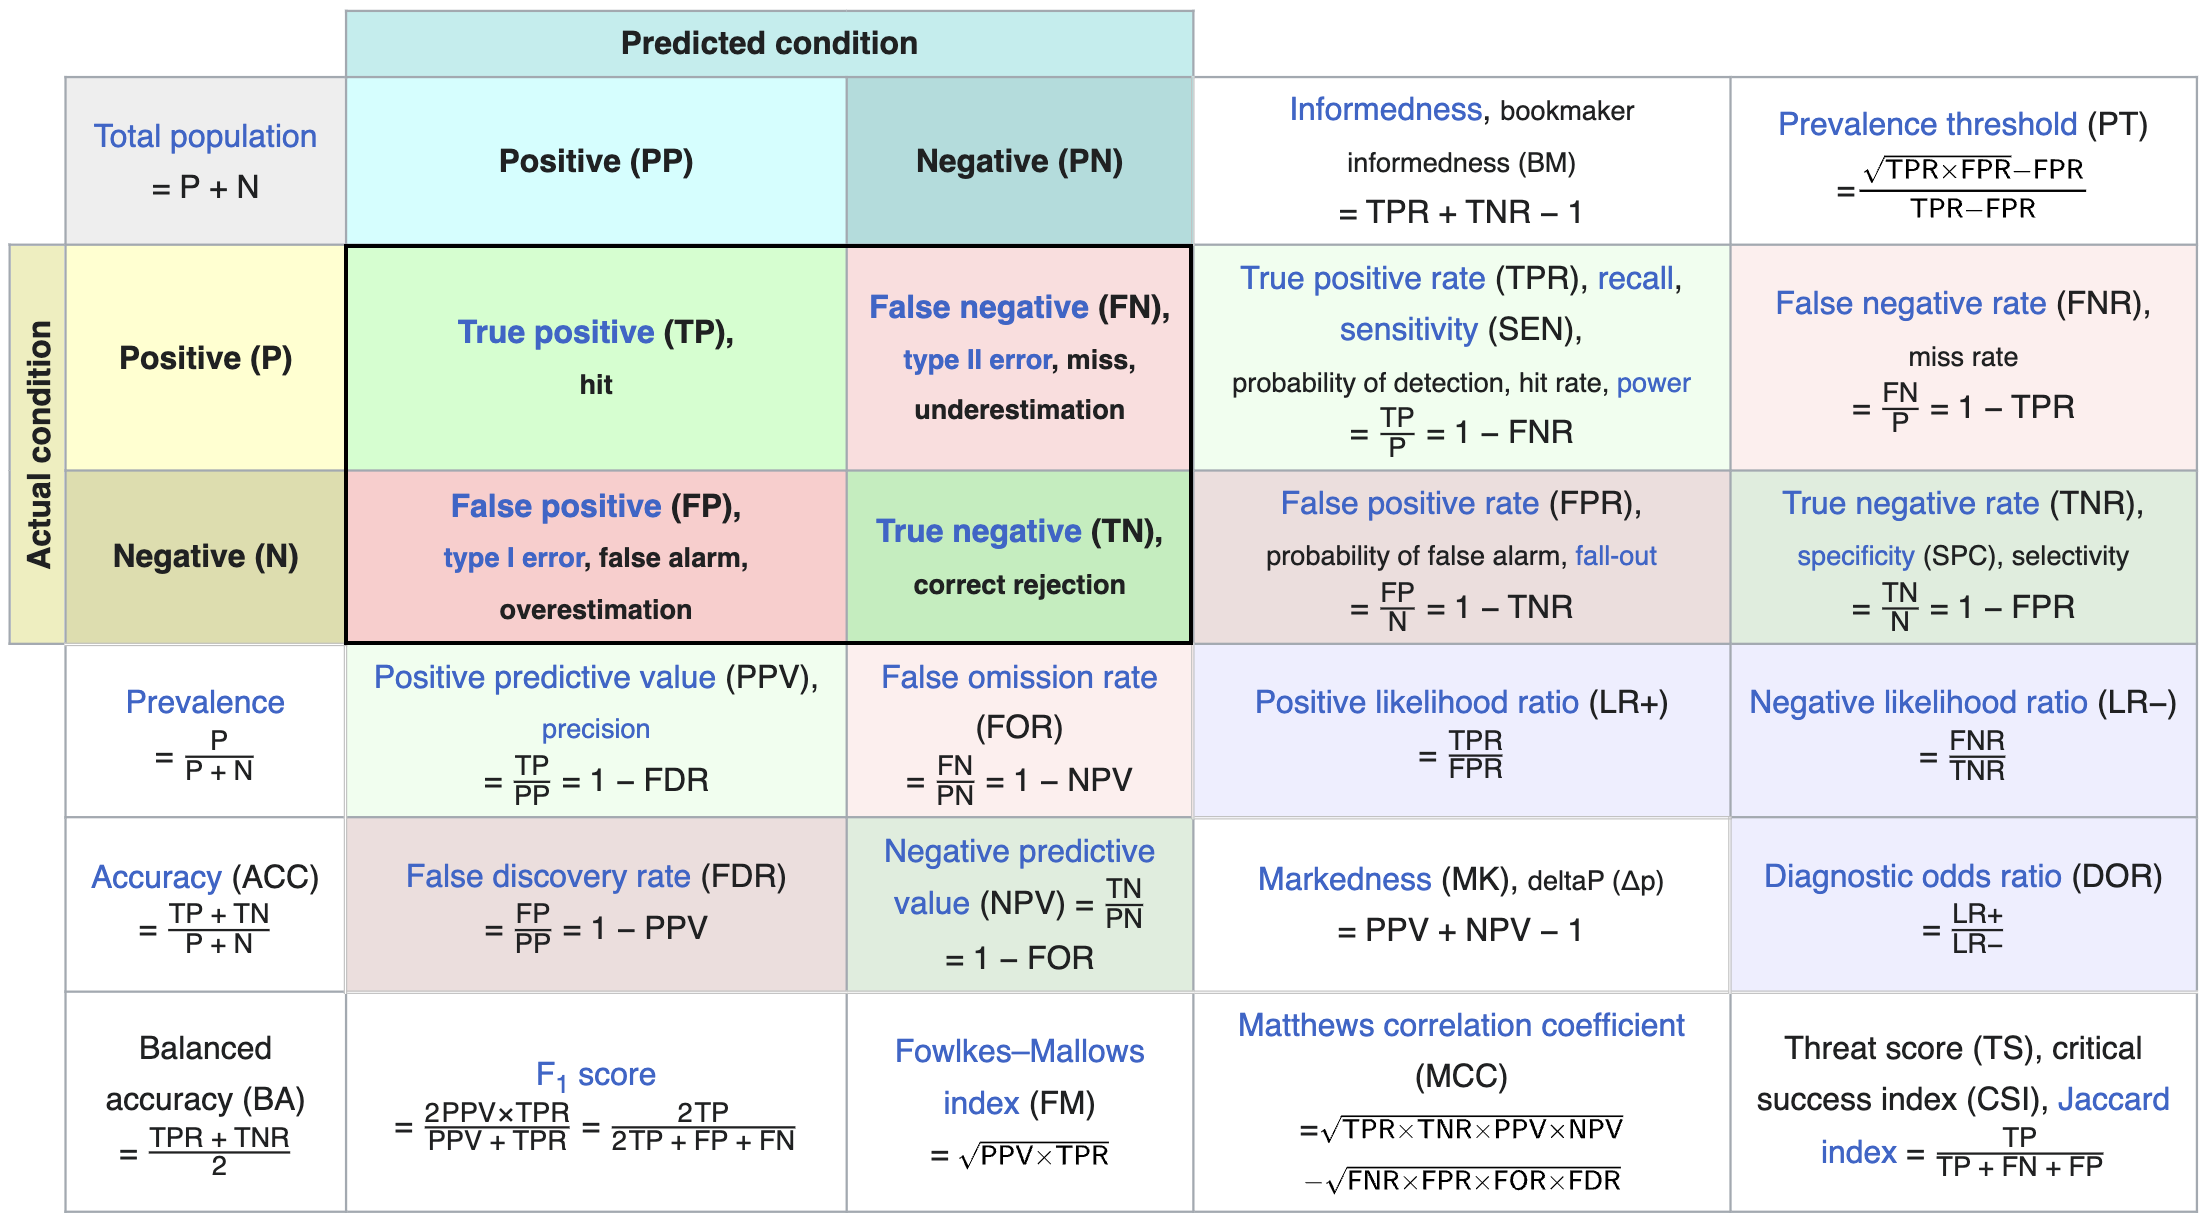
\includegraphics[width=\textwidth]{figs/confusionmtx.png}
%     \caption{Confusion matrix and the metrics defined on it}
%     {\footnotesize This table comes from Wikipedia (https://en.wikipedia.org/wiki/Confusion\_matrix).}
%     \label{fig:confusionmtx}
% \end{figure}

\begin{figure}[htpb]
    \centering
    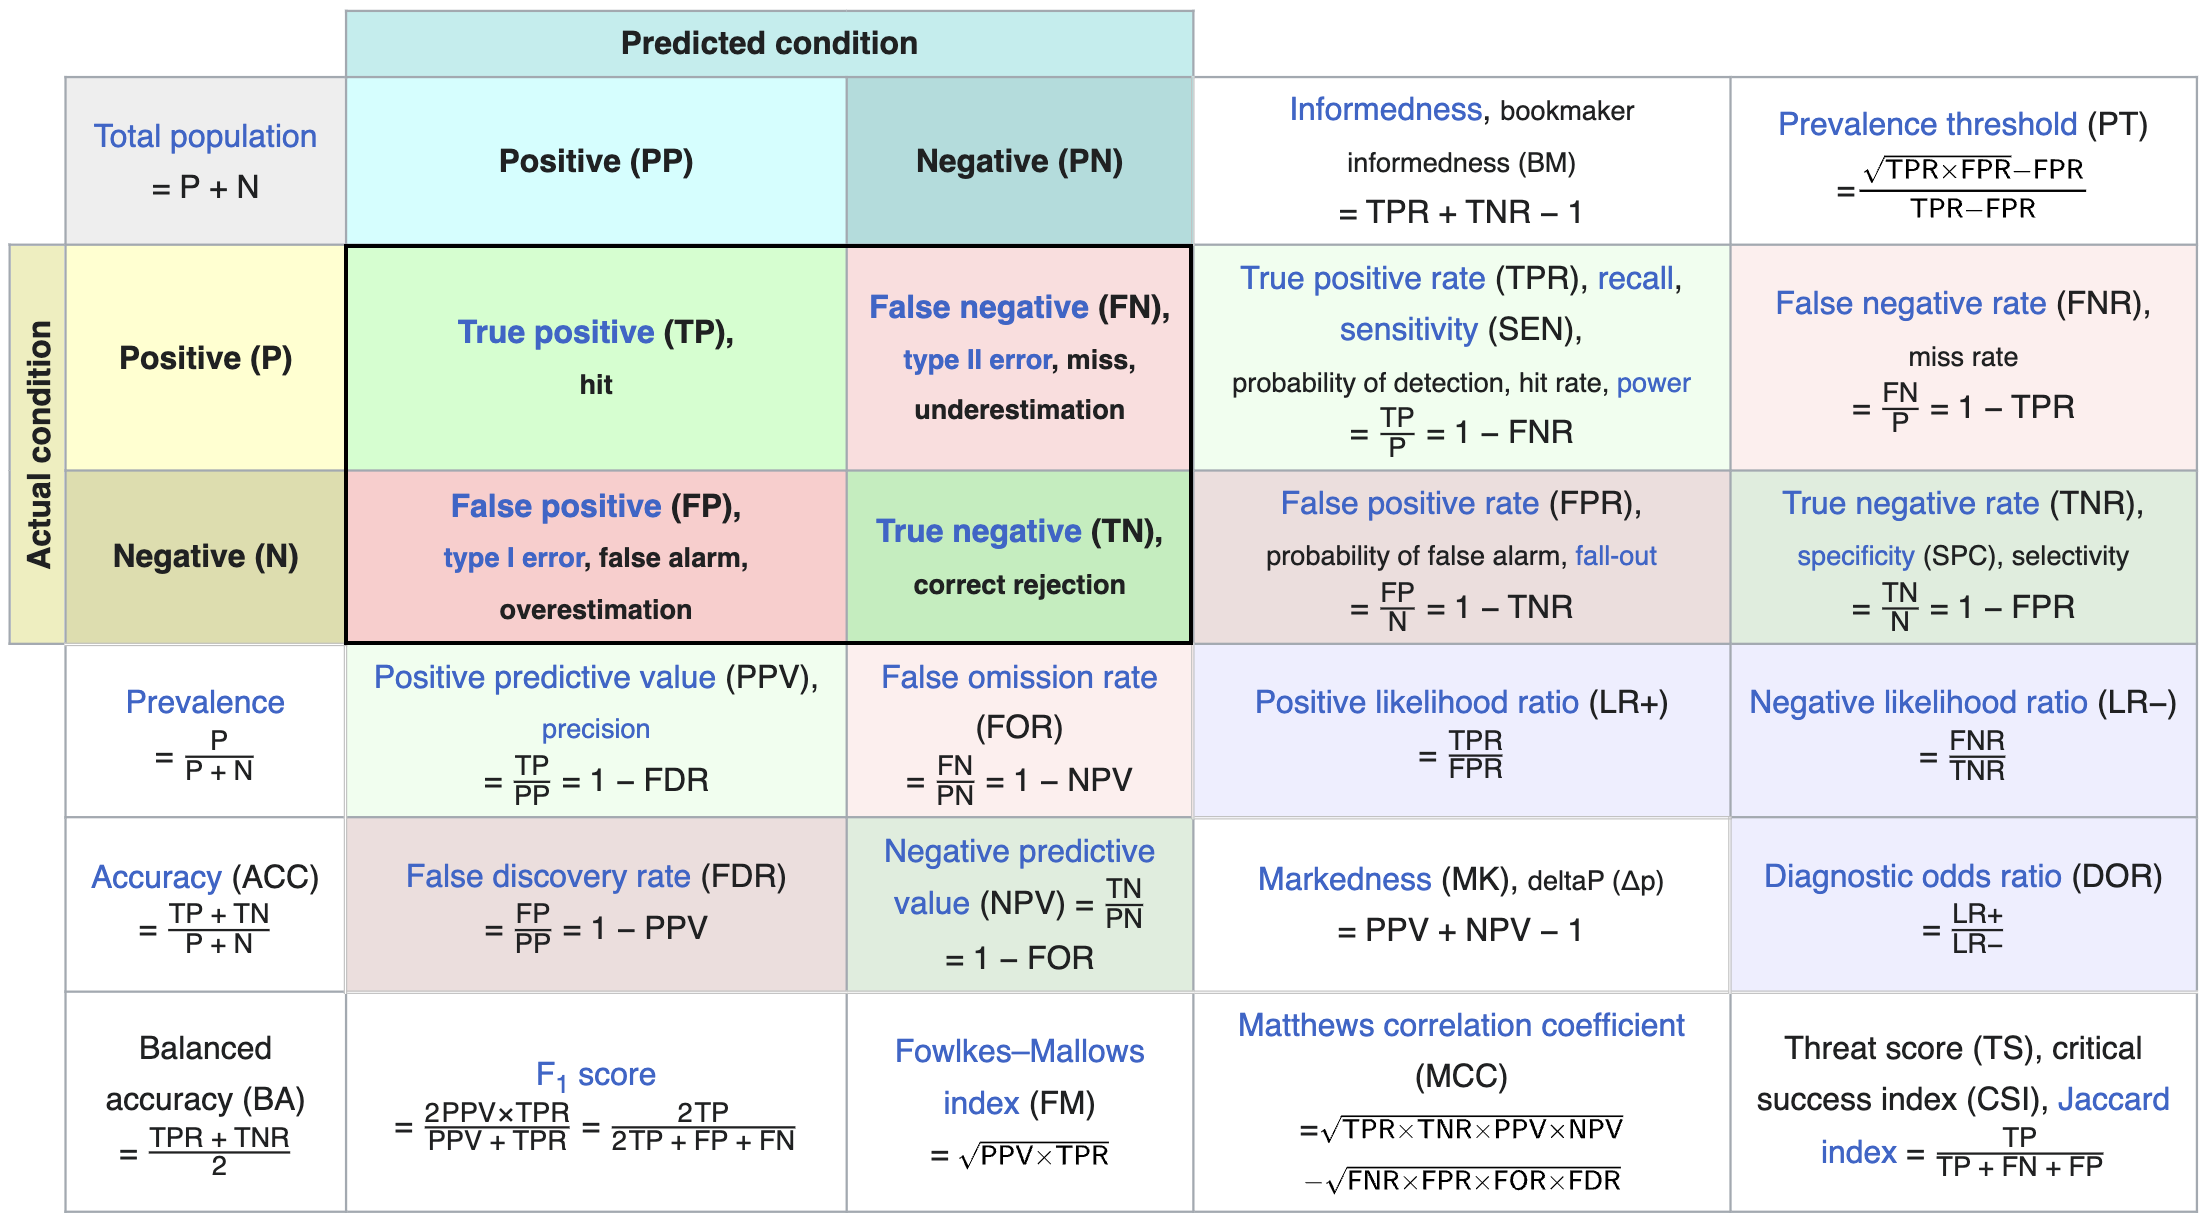
\includegraphics[width=\textwidth]{figs/confusionmtx.png}
    \caption{Confusion matrix and the metrics defined on it}
    {\footnotesize This table comes from Wikipedia (https://en.wikipedia.org/wiki/Confusion\_matrix).}
    \label{fig:confusionmtx}
\end{figure}

\textbf{Receiver operating characteristic (ROC) curves}: 
x-axis: FPR (1-Specificity) and y-axis: TPR (Recall or Sensitivity);
and \textbf{Precision-recall (PR) curves}:
x-axis: Recall and y-axis: Precision.
ROC curves (and the area under it, AUC) will not be unaffected by class imbalance,
while PR curves (and the area under \textit{interpolated} ones, AP) are sensitive to a large change in the absolute number in imbalance problem,
preferable when the shifting of absolute numbers are concerned, such as a ``negative'' is not well-defined.
 
\textbf{Huber loss}: equivalent to $\ell_2$ for errors smaller than $\delta$, 
and $\ell_1$for larger errors.
\begin{gather}
    \ell_\delta(h,a)=\left\{
    \begin{array}{ll}
        \frac{1}{2}(a-h)^2              & \text{if}~|a-h|\leq\delta\\
        \delta|a-h|-\frac{1}{2}\delta^2 & \text{if}~|a-h|>\delta
    \end{array}
    \right.
\end{gather}

\textbf{Kullback Leibler (KL) divergence}:
\begin{align}
    \infdiv{p}{q}
    \triangleq& \sum_{y\in\mathcal{Y}}p(y)\log\frac{p(y)}{q(y)}\\
    =& \underbrace{\sum_{y\in\mathcal{Y}}p(y)\log{p(y)}}_{-\mathbb{H}(p)}
        \underbrace{-\sum_{y\in\mathcal{Y}}p(y)\log{q(y)}}_{\mathbb{H}_\text{ce}(p,q)}.
\end{align}
Minimizing KL divergence between the fixed given $p$ and a $q$ is equal to find a $q$ minimizing the cross-entropy between $p$ and $q$.
$\log{\frac{p()y}{q(y)}}$ term can be quite sensitive to errors for low probability events,
so the \textbf{Brier score} an alternative
\begin{gather}
    \ell(p,q)\triangleq\frac{1}{C}\sum_{c=1}^C[q(y=c|\bm{x})-p(y=c|\bm{x})]^2
\end{gather}

\textbf{Bayes factor} for Bayesian hypothesis testing\unsure{
Recall the definition of marginal likelihood or evidence for a model $m$, 
$p(\mathcal{D}|m)=\int{p(\bm{\theta}|m)p(\mathcal{D}|\bm{\theta},m)}d\bm{\theta}$.
The model presented here is a family of distribution indexed by the parameter $\bm{\theta}$, 
so we need marginal likelihood for an average probability for family $m$ as feasible region of optimization.
}
\begin{gather}
    B_{1,0}\triangleq\frac{p(\mathcal{D}|M_1)}{p(\mathcal{D}|M_0)}
\end{gather}

\begin{table}[htbp]
    \centering
    \begin{tabular}{cl}
    \toprule
    Bayes factor $B_{0,1}$                      & Interpretation \\
    \midrule
    $(0,\frac{1}{100})$                         & Decisive evidence for $M_0$ \\
    $(\frac{1}{100},\frac{1}{10})$              & Strong evidence for $M_0$ \\
    $(\frac{1}{10},\frac{1}{3})$                & Moderate evidence for $M_0$ \\
    $(\frac{1}{3},1)$                           & Weak evidence for $M_0$ \\
    $(1,3)$                                     & Weak evidence for $M_1$ \\
    $(3,10)$                                    & Moderate evidence for $M_1$ \\
    $(10,100)$                                  & Strong evidence for $M_1$ \\
    $(100,\infty)$                              & Decisive evidence for $M_1$ \\
    \bottomrule
    \end{tabular}
    \caption{Jeffreys scale of evidence for interpreting Bayes factors}
    \label{tab:bayesfactor}
\end{table}

\textbf{Information criteria} ($D_m=|\bm{\theta}|$)
\begin{itemize}
    \item \textbf{Bayesian information criterion (BIC)}: 
    Gaussian approximation to the posterior $p(\bm{\theta}|\mathcal{D})$ with the assumptions of 
    {uniform prior ($p(\bm{\theta})\propto 1$) and iid of samples}.
    \begin{align}
        J_\text{BIC}(m)=&\log{p(\mathcal{D}|m)}\approx\log{p(\mathcal{D}|\hat{\bm{\theta}},m)-\frac{D_m}{2}\log{N}}\\
        \Rightarrow
        \mathcal{L}_\text{BIC}(m)=&-2\log{p(\mathcal{D}|\hat{\bm{\theta}},m)+D_m\log{N}}
    \end{align}
    
    \item \textbf{Akaike information criterion (AIC)}: 
    The regularization term independent of $N$ derives from a frequentist perspective.
    \begin{gather}
        \mathcal{L}_\text{AIC}(m)=-2\log{p(\mathcal{D}|\hat{\bm{\theta}},m)+2D_m}
    \end{gather}
    
    \item \textbf{Minimum description length (MDL)}:
    The bit length regularization term ($C(m)=-\log{p(m)}$) comes from the perspectives of communication cost.
    \begin{gather}
        \mathcal{L}_\text{MDL}(m)=-\log{p(\mathcal{D}|\hat{\bm{\theta}},m)+C(m)}
    \end{gather}
    
\end{itemize}

% \begin{figure}[htpb]
%     \centering
%     \begin{figure}[htpb]
    \centering
    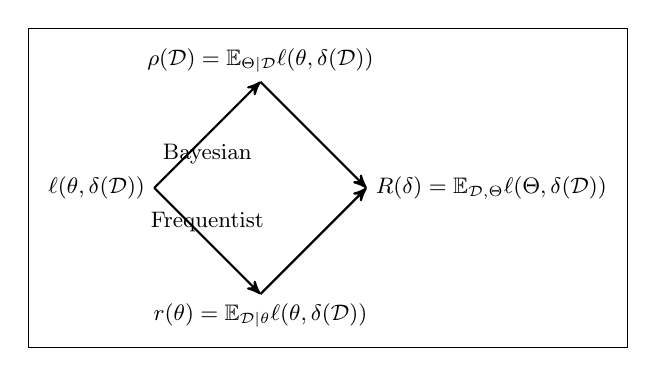
\begin{tikzpicture}[->,>=stealth',auto,node distance=3.5em,thick,show background rectangle]
    \tikzstyle{every node}=[font=\small,scale=0.9]
      \node[](anchor){};
      \node[left = of anchor]       (loss)  {$\ell(\theta,\delta(\mathcal{D}))$};
      \node[above = of anchor]          (bayes) {$\rho(\mathcal{D})=\mathbb{E}_{\Theta|\mathcal{D}}\ell(\theta,\delta(\mathcal{D}))$};
      \node[below = of anchor]         (freq)  {$r(\theta)=\mathbb{E}_{\mathcal{D}|\theta}\ell(\theta,\delta(\mathcal{D}))$};
      \node[right = of anchor]         (risk)  {$R(\delta)=\mathbb{E}_{\mathcal{D},\Theta}\ell(\Theta,\delta(\mathcal{D}))$};
      
      \draw[->] (loss.east)  --node[below]{Bayesian}     (bayes.south);
      \draw[->] (loss.east)  --node[above]{Frequentist}  (freq.north);
      \draw[->] (bayes.south) -- (risk.west);
      \draw[->] (freq.north)  -- (risk.west);
    \end{tikzpicture}
    \caption{risk from Bayesian and Frequentist perspective}
    \label{fig:riskbf}
\end{figure}
%     \caption{risk from Bayesian and Frequentist perspective}
%     \label{fig:riskbf}
% \end{figure}

\begin{figure}[htpb]
    \centering
    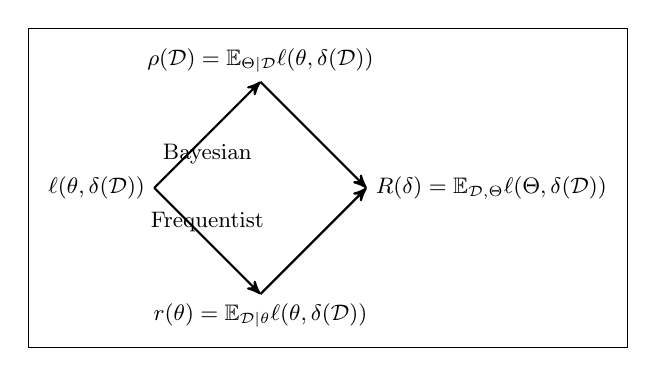
\begin{tikzpicture}[->,>=stealth',auto,node distance=3.5em,thick,show background rectangle]
    \tikzstyle{every node}=[font=\small,scale=0.9]
      \node[](anchor){};
      \node[left = of anchor]       (loss)  {$\ell(\theta,\delta(\mathcal{D}))$};
      \node[above = of anchor]          (bayes) {$\rho(\mathcal{D})=\mathbb{E}_{\Theta|\mathcal{D}}\ell(\theta,\delta(\mathcal{D}))$};
      \node[below = of anchor]         (freq)  {$r(\theta)=\mathbb{E}_{\mathcal{D}|\theta}\ell(\theta,\delta(\mathcal{D}))$};
      \node[right = of anchor]         (risk)  {$R(\delta)=\mathbb{E}_{\mathcal{D},\Theta}\ell(\Theta,\delta(\mathcal{D}))$};
      
      \draw[->] (loss.east)  --node[below]{Bayesian}     (bayes.south);
      \draw[->] (loss.east)  --node[above]{Frequentist}  (freq.north);
      \draw[->] (bayes.south) -- (risk.west);
      \draw[->] (freq.north)  -- (risk.west);
    \end{tikzpicture}
    \caption{risk from Bayesian and Frequentist perspective}
    \label{fig:riskbf}
\end{figure}

\textbf{Populaton risk}: if the true distribution $p^*{\bm{x}, \bm{y}}$ is known, 
then the risk of an estimator $f$ is 
\begin{gather}
    R(f,p^*)=R(f)\triangleq\mathbb{E}_{p^*(\bm{x},\bm{y})}\ell(\bm{y},f(\bm{x})).
\end{gather}
Of course, $p^*$ is unknown, 
but we can approximate it using the \textit{empirical distribution} with $N$ samples
and get \textbf{empirical risk}\unsure{
This distribution is discrete. 
If there are some new data point $(\bm{x},\bm{y})$ that haven't occur in dataset,
then, $p\mathcal{D}(\bm{x},\bm{y})=0$,
so it will need some smoothing method or, directly, use empirical expectation that averages over the observed data points.
Empirical risk minimization widely applied in training a deep learning model, 
and the hypothesis space $\mathcal{H}$ depends on the architecture of model.
}
\begin{gather}
    p_{\mathcal{D}}(\bm{x},\bm{y})
    \triangleq
    \frac{1}{|\mathcal{D}|}\sum_{(\bm{x}_n,\bm{y}_n)\in\mathcal{D}}\delta(\bm{x}-\bm{x}_n)\delta(\bm{y}-\bm{y}_n) \\
    R(f,\mathcal{D})
    \triangleq
    \mathbb{E}_{p_{\mathcal{D}}(\bm{x},\bm{y})}\ell(\bm{y},f(\bm{x}))=\frac{1}{N}\sum_{n=1}^N\ell(\bm{y}_n,f(\bm{x}_n))\\
    \hat{f}_\mathcal{D}=\argmin_{f\in\mathcal{H}}R(f,\mathcal{D}).
\end{gather}
Due to \uline{approximation of true distribution (from data)} and \uline{limitation of tractable hypothesis space (from model)}, 
there will exist errors between empirically optimal estimator $\hat{f}_\mathcal{D}$ and universally optimal estimator $f^{**}$
\begin{gather}
    f^{**}=\argmin_f R(f),~
    f^*=\argmin_{f\in\mathcal{H}} R(f),~
    f^*_{\mathcal{D}_\text{tr}}=\argmin_{f\in\mathcal{H}}R(f,\mathcal{D}_\text{tr})\\
    \mathbb{E}_{p^*}\left[R(f^*_{\mathcal{D}_\text{tr}})-R(f^{**})\right]
    =\underbrace{R(f^*)-R(f^{**})}_{\mathcal{E}_\text{app}(\mathcal{H})}
    +\underbrace{\mathbb{E}_{p^*}\left[R(f^*_{\mathcal{D}_\text{tr}})-R(f^*)\right]}_{\mathcal{E}_\text{est}(\mathcal{H,\mathcal{D}_\text{tr}})}\\
    % \mathbb{E}_{p^*}\left[R(f^*_{\mathcal{D}_\text{tr}})-R(f^*)\right]
    \mathcal{E}_\text{est}(\mathcal{H,\mathcal{D}_\text{tr}})
    = \mathbb{E}_{p_\text{tr}}\ell{(\bm{y},f^*_{\mathcal{D}_\text{tr}}(\bm{x}))}
    - \mathbb{E}_{p_\text{te}}\ell{(\bm{y},f^*_{\mathcal{D}_\text{tr}}(\bm{x}))} + \varepsilon_\text{gen}
\end{gather}
where 
$\mathcal{E}_\text{app}(\mathcal{H})$ is approximation error, 
$\mathcal{E}_\text{est}(\mathcal{H,\mathcal{D}_\text{tr}})$ is estimation/generalization error,
and $\varepsilon_\text{gen}$ is called generalization gap.

\textbf{Structural risk minimization}: minimized the regularized \textit{population} risk to pick a model of right complexity.
\begin{gather}
    \argmin_\lambda\min_{\bm{\theta}}\{R(\bm{\theta})+\lambda C(\bm{\theta})\}
\end{gather}
The empirical risk ignored the risk caused by unobserved data and underestimates the population risk,
and the minimization regularized empirical risk 
\begin{gather}
    R_\lambda(\bm{\theta},\mathcal{D})\triangleq R(\bm{\theta},\mathcal{D})+\lambda C(\bm{\theta})
\end{gather} 
always results in $\lambda=0$.
\begin{itemize}
    \item \textbf{cross-validation}\unsure{In the context of DL, $\lambda$ may be the number of training epochs.}
    \begin{gather}
        \hat{\bm{\theta}}_\lambda(\mathcal{D}_\text{tr})=\argmin_{\bm{\theta}}R_\lambda(\bm{\theta},\mathcal{D}_\text{tr}) \\
        R_\lambda^\text{val}\triangleq R(\hat{\bm{\theta}}_\lambda(\mathcal{D}_\text{tr}),\mathcal{D}_\text{val}),~\text{and}~
        R_\lambda^\text{cv}\triangleq\frac{1}{K}\sum_{k=1}^K{R(\hat{\bm{\theta}}(\mathcal{D}_{K\setminus k}),\mathcal{D}_k)} \\
        \hat{\lambda}=\argmin_\lambda R_\lambda^\text{cv} \\
        \hat{\bm{\theta}}=\argmin_{\bm{\theta}}R_{\hat{\lambda}}(\bm{\theta},\mathcal{D})
    \end{gather}\unsure{In real application, 
    the K model snapshots with the optimal $\hat{\lambda}$ during training process may be ensembled, 
    such as average the predictions,
    to a final model, instead of retrained on the entire dataset, 
    because of the additional cost in running time and resources of computation or storage.}
    \item \textbf{statistical learning theory}: Theorem \ref{thm:boundgenerror} tells us the gap between 
    empirical risk and population risk has an upper bound with some probability. 
    The prediction by the model that reach the upper bound is called \textbf{probability approximately correct},
    when the hypothesis class $\mathcal{H}$ is \textbf{PAC learnable}. 
\end{itemize}

\begin{theorem}\label{thm:boundgenerror}
    \textbf{{Upper bound of generalization risk}}\\
    For any data distribution $p^*$ and nay dataset $\mathcal{D}$ of size $N$ drawn from $p^*$,
    the probability that the \uline{generalization error of a binary classifier selected from a finite hypothesis class $\mathcal{H}$} 
    will be more that $\epsilon$.
    In the worst case, it is upper bounded as follows:
    \begin{gather}
        P\left(
            \max_{h\in\mathcal{H}}{|R(h)-R(h,\mathcal{D})|}>\epsilon
        \right)
        \leq 2\mathrm{dim}(\mathcal{H})\exp\{-2N\epsilon^2\}
    \end{gather}
    where $R(h,\mathcal{D})=\frac{1}{N}\sum_{n=1}^N \mathbb{I}(f(\bm{x}_n)\neq y_n)$ empirical risk, 
    $R(h)=\mathbb{E}_{p^*(\bm{x},y)}\mathbb{I}(f(\bm{x})\neq y)$ population risk, 
    and $\mathrm{dim}(\mathcal{H})=|\mathcal{H}|$.
    When the hypothesis class is infinite, we take $\mathrm{dim}(\mathcal{H})=\mathrm{dim}_\text{VC}(\mathcal{H})$,
    \textbf{VC dimension}, measuring the degrees of freedom of the hypothesis class.
    
    \textit{Remark}: the more data the less error; the larger hypothesis space the more error.
\end{theorem}


\subsection{Information Theory}

% \begin{figure}[htpb]
%     \centering
%     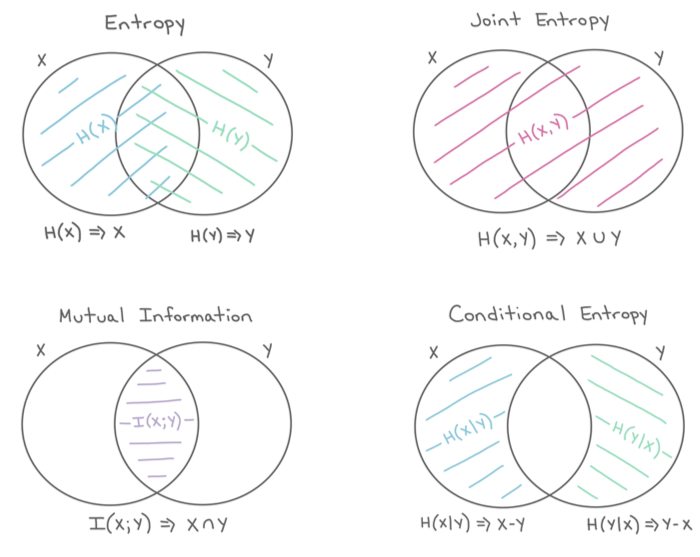
\includegraphics[width=0.6\textwidth]{figs/entropy.png}
%     \caption{The marginal entropy, joint entropy, conditional entropy and mutual information represented as information diagrams.}
%     \label{fig:entropy}
% \end{figure}

\begin{figure}[htpb]
    \centering
    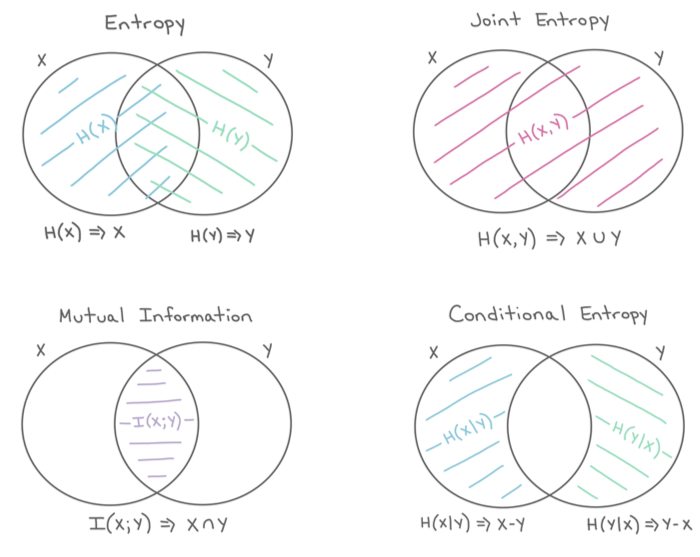
\includegraphics[width=0.6\textwidth]{figs/entropy.png}
    \caption{The marginal entropy, joint entropy, conditional entropy and mutual information represented as information diagrams.}
    \label{fig:entropy}
\end{figure}

\textbf{Cross entropy}: expected number of bits needed to compress some data
samples drawn from distribution $p$ using a code based on distribution $q$,
and the optimal code is reached by $q=p$, i.e., the entropy of $p$ \textbf{(Shannon's source coding theorem)}.
\begin{gather}
    \mathbb{H}(p,q)\triangleq-\sum_{k=1}^K p_k\log_2{q_k}\ge\mathbb{H}(p)
\end{gather}
The continuous version is called \textbf{differetial entropy}
\begin{gather}
    h(X)\triangleq-\int_{\mathcal{X}}p(x)\log{p(x)}dx,
\end{gather}
which can be negative and 
all real-valued quantities can be \uline{represented to finite precision}, 
says, \uline{$n$-bit} \textbf{quantization}, \unsure{Note it is not $B$-bin}
and the approximated discrete value's entropy will be $h(X)+n$. 
One simple approach to discretize is to bin the distribution based on its \uline{empirical quantiles} and the number of bins is determined by 
\begin{gather}
    B=N^\frac{1}{3}\frac{\max{D}-\min{D}}{3.5\sigma_\mathcal{D}}.
\end{gather}

\textbf{Joint entropy} of two random variables $X$ and $Y$
\begin{gather}
    \mathbb{H}(X,Y)=-\sum_{x\in\mathcal{X},y\in\mathcal{Y}}p(x,y)\log_2 p(x,y)\\
    0 \leq \max\{\mathbb{H}(X),\mathbb{H}(Y)\} \leq \mathbb{H}(X,Y) \leq \mathbb{H}(X) + \mathbb{H}(Y)
\end{gather}
where the right equality holds if $X$ \rotatebox{90}{$\models$} $Y$,
which says combining variables together does not make the entropy go down: you cannot
reduce uncertainty merely by adding more unknowns to the problem, you need to observe some data,
and if there is no information introduced by the additional unknowns, the system will reach the maximum chaos.

\textbf{Conditional entropy} of $Y$ given $X$ is the uncertainty we have in $Y$ after seeing $X$, averaged
over possible values for $X$
\begin{align}
    \mathbb{H}(Y|X)
    =& -\sum_{x\in\mathcal{X}}p(x)\sum_{y\in\mathcal{Y}}p(y|x)\log{p(y|x)} \\
    =& -\sum_{x\in\mathcal{X},y\in\mathcal{Y}}p(x,y)\log{\frac{p(x,y)}{p(x)}} \\
    =& \mathbb{H}(X,Y)-\mathbb{H}(X)
\end{align}
\begin{gather}
    0 \leq \mathbb{H}(Y|X) \leq \mathbb{H}(Y)
\end{gather}
where the left equality holds if $Y=f(X)$ where $f$ is deterministic, 
and the right equality holds if $X$ \rotatebox{90}{$\models$} $Y$,
which says that, \textit{on average}, conditioning on data never increases one’s uncertainty.
\begin{gather}
    \mathbb{H}(X_1,\cdots,X_n)=\sum_{i=1}^n{\mathbb{H}(X_i|X_1,\cdots,X_{i-1})}
\end{gather}

\textbf{Relative entropy} or KL divergence\unsure{
already introduced in Chapters 2 and 5.
} measures the (asymmetric) distance between two distributions, which can be interpreted as a lower bound on the number of bits (or ``extra number of bits'') needed to compress data coming from distribution $p$ based on $q$ as the basis of coding scheme.
\begin{align}
    \infdiv{p}{q}
    \triangleq& \sum_{y\in\mathcal{Y}}p(y)\log\frac{p(y)}{q(y)}\\
    =& \sum_{y\in\mathcal{Y}}p(y)\log{p(y)} -\sum_{y\in\mathcal{Y}}p(y)\log{q(y)} \\
    =& -\mathbb{H}(p) + \mathbb{H}_\text{ce}(p,q)
\end{align}

\begin{corollary}
    \textbf{Uniform distribution maximizes the entropy}\\
    $\mathbb{H}(X)\leq\log{|\mathcal{X}|}$, where $|\mathcal{X}|$ is the number of states for $X$, with equality iff $p(x)$ is uniform.
\end{corollary}
\begin{proof}
    Let $u(x)=\frac{1}{|\mathcal{X}|}$, then
    \begin{gather}
        0\leq\infdiv{p}{u}=\sum_{x\in\mathcal{X}}p(x)\log{\frac{p(x)}{q(x)}}=\log{|\mathcal{X}|-\mathbb{H}(X)}
    \end{gather}
\end{proof}

\textbf{Mutual information} measures the dependence of two random variables or the similarity of two distributions, which can serve as a generalized correlation coefficient
\begin{gather}
    \mathbb{I}(X;Y)\triangleq\infdiv{p(x,y)}{p(x)p(y)}
    =\sum_{x\in\mathcal{X}}\sum_{y\in\mathcal{Y}}p(x,y)\log\frac{p(x,y)}{p(x)p(y)}\geq 0
\end{gather}
where the right equality holds iff $X\vperp Y$ and MI approaches $\infty$ if $Y$ tells us an infinite amount of information about $X$.
\begin{align}
    \mathbb{I}(X;Y)
    =& \mathbb{H}(X)-\mathbb{H}(X|Y) \\
    =& \mathbb{H}(Y)-\mathbb{H}(Y|X) \\
    =& \mathbb{H}(X,Y)-\mathbb{H}(X|Y)-\mathbb{H}(Y|X) \\
    =& \mathbb{H}(X) + \mathbb{H}(Y) - \mathbb{H}(X,Y)
\end{align}
\textbf{Conditional mutual information} is the extra information that 
$X$ tells us about $Y$, excluding what we already knew about $Y$ given $Z$ alone.
\begin{align}
    \mathbb{I}(X;Y|Z)
    \triangleq& \mathbb{E}_{p(z)}[\mathbb{I}(X;Y)|Z] \\
    =& \mathbb{E}_{p(z,y,z)}\frac{p(x,y|z)}{p(x|z)p(y|z)} \\
    =& \mathbb{I}(Y;X,Z)-\mathbb{I}(Y;Z)
\end{align}
\textbf{Normalized mutual information (NMI)}: normalize the MI into $[0,1]$, served as ``modern correlation coefficient''
\begin{gather}
    \mathrm{NMI}(X,Y)=\frac{\mathbb{I}(X;Y)}{\min\{\mathbb{H}(X),\mathbb{H}(Y)\}}\in[0,1]
\end{gather}
which need a \uline{discretization technique} to make the \uline{computation tractable}:
\textbf{Maximal information coefficient}
\begin{gather}
    \mathrm{MIC}(X,Y)=\max_{G}\frac{I((X,Y)|_G)}{\log\|G\|}\approx\mathrm{NMI}(X,Y)
\end{gather}
where $G$ is a set of 2D grids, $(X,Y)|_G$ represents a 2D discretization of $X$ and $Y$,
$\|G\|\triangleq\min\{G_x,G_y\}$, $G_x$ is the number of grid cells in the $x$ direction, so be $G_y$.

\begin{theorem}
    \textbf{Data processing inequality}\\
    Suppose $X\to Y\to Z$ forms a Markov chain, so that $X\vperp Z|Y$.
    Then $\mathbb{I}(X;Y)\geq\mathbb{I}(X;Z)$.
\end{theorem}
\begin{proof}
    \begin{align}
        \mathbb{I}(X;Y,Z)
        =& \mathbb{I}(X;Z)+\mathbb{I}(X;Y|Z)\\
        =& \mathbb{I}(X;Y)+\mathbb{I}(X;Z|Y)
    \end{align}
    \begin{gather}
        X\vperp Z|Y\Rightarrow \mathbb{I}(X;Z|Y)=0\\
        \Rightarrow \mathbb{I}(X;Z)+\underbrace{\mathbb{I}(X;Y|Z)}_{\geq 0}=\mathbb{I}(X;Y) \\
        \Rightarrow \mathbb{I}(X;Y)\geq\mathbb{I}(X;Z)
    \end{gather}
    Similarly,
    \begin{gather}
        \mathbb{I}(Y;Z)\geq\mathbb{I}(X;Z)
    \end{gather}
\end{proof}


% \begin{framed}{\large
% TODO list of the following week
% \begin{itemize}
%     \item Finish the note organization work of Part II
%     \item Read Chapters 9 and 10
%     \item Course works
% \end{itemize}
% }
% \end{framed}





% ############################### WK 3 #######################################

% \setcounter{section}{2}
% \setcounter{subsection}{6}
% \begin{center}
% \textit{Chapter 7 Linear Algebra \& Chapter 8 Optimization $\S$ 1-5.}
% \end{center}

% % \subsection{Decision Theory}

% \subsection{Information Theory}


\setcounter{subsection}{6}
\subsection{Linear Algebra}

\begin{table}[htpb]
    \centering
    \begin{tabular}{rp{32em}}
        \toprule
        Terminology & Brief definition\\
        \midrule
        \textbf{span} of vectors &  $\text{span}(\{\bm{x}_1,\cdots,\bm{x}_n\})\triangleq\left\{\bm{v}:\bm{v}=\sum_{i=1}^n\alpha_i\bm{x}_i,\alpha_i\in\mathbb{R}\right\}$\\
        \textbf{range} of a matrix & $\text{range}(\mathbf{A})\triangleq\{\bm{v}=\mathbf{A}\bm{x}\}$, column space \\ 
        \textbf{nullspace} of a matrix & $\text{nullspace}(\mathbf{A})\triangleq{\{\bm{x}:\mathbf{A}\bm{x}=\bm{0}\}}$\\
        \textbf{projection} & $\text{Proj}(\bm{y};\{\bm{x}_1,\cdots,\bm{x}_n\})=\argmin_{\bm{v}\in\text{span}(\{\bm{x}_1,\cdots,\bm{x}_n\})}\|\bm{y}=\bm{v}\|_2$ 
        or if $\mathbf{A}$ full rank in columns $\text{Proj}(\bm{y};\mathbf{A})=\mathbf{A}(\mathbf{A}^T\mathbf{A})^{-1}\mathbf{A}^T\bm{y}$ \\
        \textbf{max-norm} and \textbf{0-norm} & $\|\bm{x}\|_\infty=\max|x_i|$ and $\|\bm{x}\|_0=\sum_{i=1}^n\mathbb{I}(x_i\neq 0)$\\
        \bottomrule
    \end{tabular}
    \caption{Gleanings of linear algebra concepts}
    \label{tab:linalgc}
\end{table}

\textbf{Induced norm} of a matrix:\unsure{
recall that the \textbf{norm of a vector} is a measure of the vector's length or magnitude
and singular value of a matrix is }
The maximum response of a linear function by unite-norm input
\begin{gather}
    \|\mathbf{A}\|_p=\max_{\bm{x}\neq\bm{0}}\frac{\|\mathbf{A}\bm{x}\|_p}{\|\bm{x}\|_p}=\max_{\|\bm{x}\|_p=1}\|\mathbf{A}\bm{x}\|_p
\end{gather}


% \subsection{Optimization}

% \begin{figure}[htpb]
    \centering
    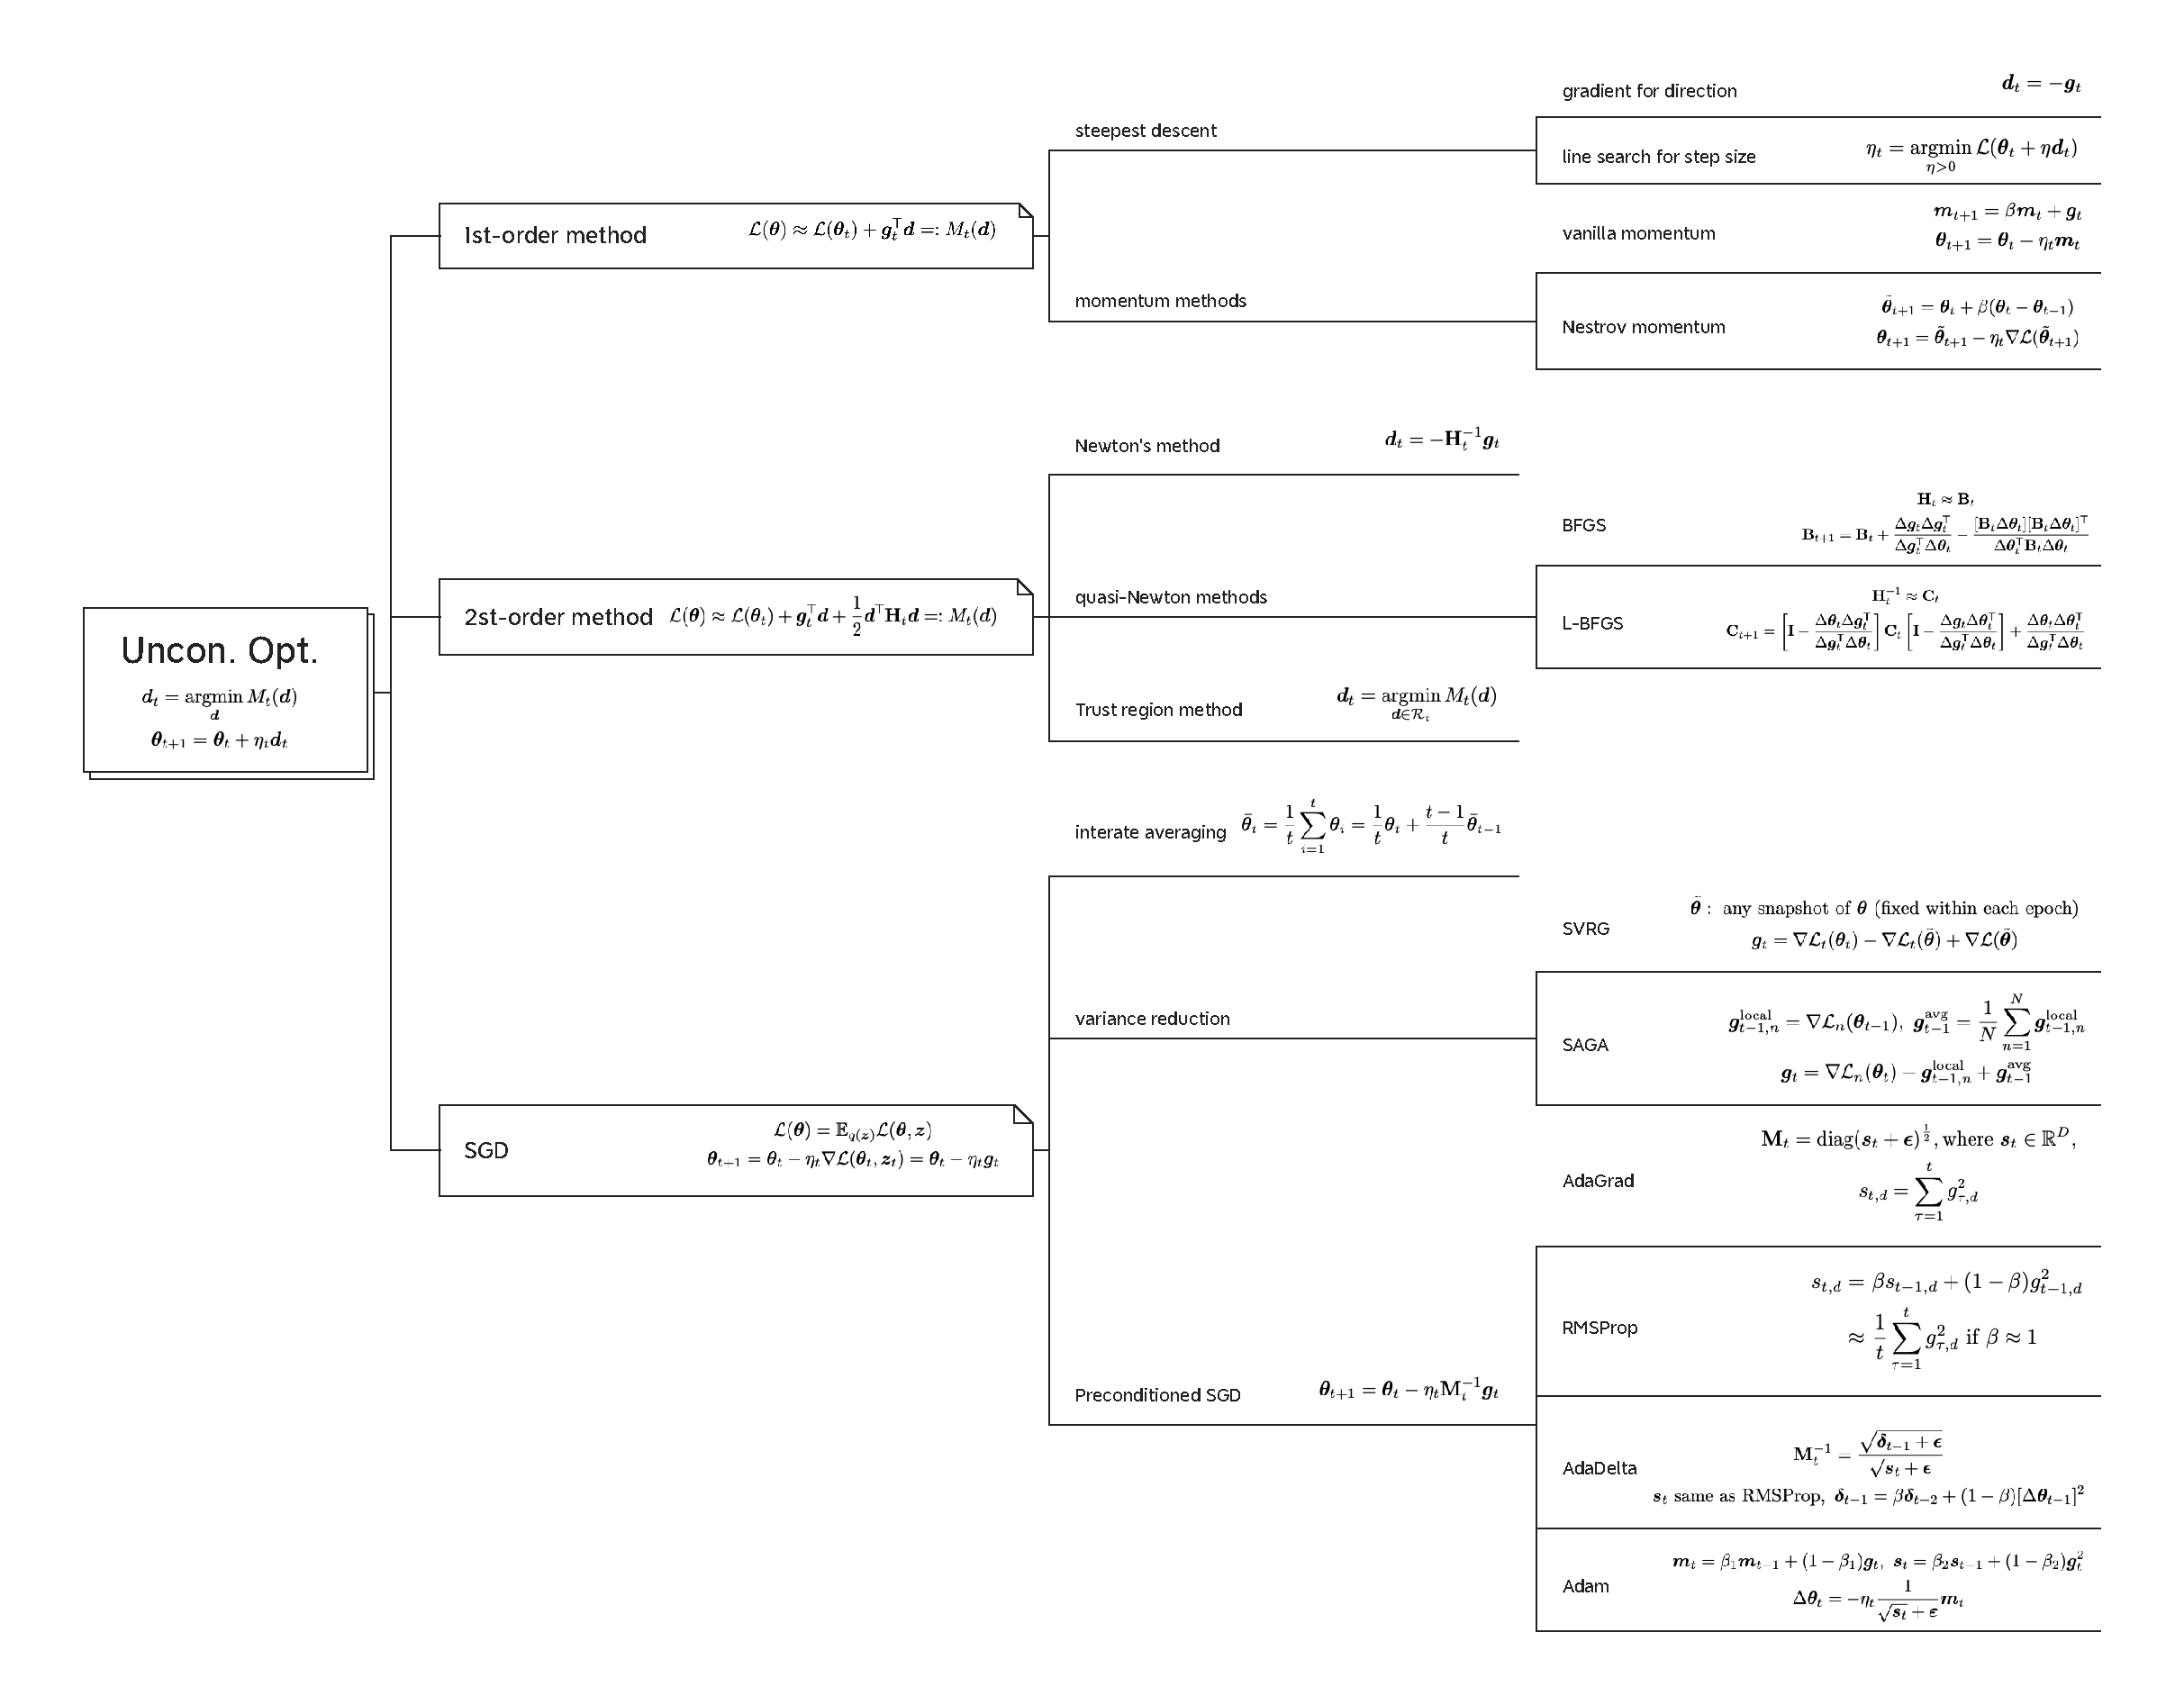
\includegraphics[width=\textwidth]{figs/unconopt.pdf}
    \caption{Solutions for unconstrained optimization updating strategies}
    {\footnotesize there are approximation methods for $M_t(\bm{d})$ and $\bm{d}_t$.
    \textbf{BFGS}: Broyden, Fletcher, Goldfarb and Shanno;
    \textbf{L-BFGS}: limited memory BFGS;
    \textbf{SGD}: Stochastic Gradient Descent;
    \textbf{SVRG}: Stochastic Variance Reduced Gradient;
    \textbf{SAGA}: Stochastic Averaged Gradient Accelerated;
    \textbf{AdaGrad}: ADAptive Gradient;
    \textbf{RMSProp}: Root Mean Squared resilient PROPagation;
    \textbf{Adam}: Adaptive moment estimation.
    }
    
    \label{fig:unconopt}
\end{figure}

% \textit{Handwriting notes were put on the book directly.\\
% To be continue...}

% \begin{framed}{\large
% TODO list of the following two weeks
% \begin{itemize}
%     \item Organize the reading notes and read the remained $\S$ 8.6-8.8, especially EM algorithm;
%     \item Read Chapters 5 and 6 (Decision Theory $\And$ Information Theory);
%     \item Course works:
%     \begin{enumerate}
%         \item homework of Linear Model (5030),
%         \item Read reference books of Multivariable Analysis (5020),
%         \item Exercises of Probability $\And$ Inference.
%     \end{enumerate}
% \end{itemize}
% }
% \end{framed}





% ############################### WK 6 #######################################

% \setcounter{section}{2}
% \begin{center}
% \textit{Chapters 9 Linear Discriminant Analysis, 10 Logistic Regression, 11 Linear Regression, and 12 Generalized Linear Models.}
% \end{center}

% \section{Linear Models}

\begin{quote}
    \citep{pml1Book} -- Chapters 9-12.
\end{quote}

\subsection{Linear Discriminant Analysis}

\textbf{Generative classifier}: 
modeling that the features are generated from \textbf{class conditional density} $p(\bm{x}|y=c;\bm{\theta})$
\begin{gather}
    % p(y)=\mathrm{Cat}(y|\bm{\pi})\\
    p(y=c|\bm{x};\bm{\theta})=
    \frac{{\color{red}p(\bm{x}|y=c;\bm{\theta})}{\color{blue}p(y=c;\bm{\theta})}}
    {\sum_{c'\in\mathcal{C}}p(\bm{x}|y=c';\bm{\theta})p(y=c';\bm{\theta})}\\
    % \underbrace{
    % \log{p(y=c|\bm{x};\bm{\theta})}=[\bm{w}(\bm{\theta})]^\mathsf{T}\bm{x}+\text{const}}_\text{LDA}
    % ~\text{for some special}~p(\bm{x}|y=c;\bm{\theta})
\end{gather}
\textbf{discriminative classifier}: classifying the samples directly by modeling $p(y|\bm{x},\bm{\theta})$ directly.
\begin{itemize}
    \item \textbf{Gaussian discriminant analysis} $p(\bm{x}|y=c;\bm{\theta})=\mathcal{N}(\bm{x}|\bm{\mu}_c,\bm{\Sigma}_c)$
\end{itemize}\unsure{
\color{red}What special class conditional density?
}

\textbf{Gaussian discriminant analysis}: 
\begin{align}
    p(y) =&~ \mathrm{Cat}(y|\bm{\pi})\\
    p(\bm{x}|y=c;\bm{\theta})
    =&~ \mathcal{N}(\bm{x}|\bm{\mu}_c,\bm{\Sigma}_c)\\
    =&~ (2\pi)^{-\frac{D}{2}}|\bm{\Sigma}_c|^{-\frac{1}{2}}\exp\left\{
        -\frac{1}{2}(\bm{x}-\bm{\mu}_c)^\mathsf{T}\bm{\Sigma}_c^{-1}(\bm{x}-\bm{\mu}_c)
    \right\}
\end{align}

\textbf{Quadratic decision boundaries}: 
for $\text{unspecified}~\bm{\Sigma}_c$
\begin{align}
    \log{p(y=c|\bm{x},\bm{\theta})}
    =&~ \log{\pi_c}-\frac{1}{2}\log|2\pi\bm{\Sigma}_c| \\
      -&~ \boxed{\frac{1}{2}(\bm{x}-\bm{\mu}_c)^\mathsf{T}\bm{\Sigma}_c^{-1}(\bm{x}-\bm{\mu}_c)}
      + \text{const}
\end{align}

\textbf{Linear decision boundaries}: 
for $\bm{\Sigma}_c=\bm{\Sigma}~(\text{shared}~\bm{\Sigma})$
\begin{align}
    \log{p(y=c|\bm{x},\bm{\theta})}
    =&~ \overbrace{
        \log{\pi_c} - \frac{1}{2}\bm{\mu}_c^\mathsf{T}\bm{\Sigma}^{-1}\bm{\mu}_c
    }^{\gamma_c} \\
    +&~ \boxed{
        \bm{x}^\mathsf{T}\underbrace{\bm{\Sigma}^{-1}\bm{\mu}_c}_{\bm{\beta}_c}
    }
    + \underbrace{
        \text{const} - \frac{1}{2}\bm{x}^\mathsf{T}\bm{\Sigma}^{-1}\bm{x}
    }_{\kappa}
\end{align}

\textbf{Logistic Regression}:
\begin{align}
    p(y=c|\bm{x},\bm{\theta})
    =&~ \frac{\exp\{\bm{\beta}_c^\mathsf{T}\bm{x}+\gamma_c\}}{\sum_{c'}\exp\{\bm{\beta}_{c'}^\mathsf{T}\bm{x}+\gamma_{c'}\}} \\
    =&~ \frac{\exp\{\bm{w}_c^\mathsf{T}[1,\bm{x}]\}}{\sum_{c'}\exp\{\bm{w}_{c'}^\mathsf{T}[1,\bm{x}]\}}
\end{align}
If $C=2$, we have 
\begin{align}
    p(y=1|\bm{x},\bm{\theta}) 
    =&~ \sigma\left((\bm{\beta}_1-\bm{\beta}_0)^\mathsf{T}\bm{x}+(\gamma_1-\gamma_0)\right)\\
    =&~ \sigma(\bm{w}^\mathsf{T}(\bm{x}-\bm{x}_0))\\
    \bm{w} =&~ \bm{\beta}_1-\bm{\beta}_0 = \bm{\Sigma}^{-1}(\bm{\mu}_1-\bm{\mu}_0) \\
    \bm{x}_0 =&~ \frac{1}{2}(\bm{\mu}_1 + \bm{\mu}_0) 
        - (\bm{\mu}_1 - \bm{\mu}_0)
        \frac{\log(\pi_1/\pi_0)}
        {(\bm{\mu}_1 - \bm{\mu}_0)^\mathsf{T}\bm{\Sigma}^{-1}(\bm{\mu}_1 - \bm{\mu}_0)}
\end{align}


\textbf{MLE}:
\begin{align}
    \hat{\bm{\mu}}_c =&~ \frac{1}{N_{\mathcal{D}}}\sum_{n:y_n=c}\bm{x}_n \\
    \hat{\bm{\Sigma}}_c =&~ \frac{1}{N_{\mathcal{D}_c}}\sum_{n:y_n=c}
    \left(\bm{x}_n-\hat{\bm{\mu}}_c\right)\left(\bm{x}_n-\hat{\bm{\mu}}_c\right)^\mathsf{T}
\end{align}

\textbf{Tied covariance}:
\begin{align}
    \hat{\bm{\Sigma}}
    =&~ \frac{1}{N_{\mathcal{D}}}\sum_{c=1}^C\sum_{n:y_n=c}
    \left(\bm{x}_n-\hat{\bm{\mu}}_c\right)\left(\bm{x}_n-\hat{\bm{\mu}}_c\right)^\mathsf{T} \\
    =&~ \sum_{c=1}^C\frac{N_{\mathcal{D}_c}}{N_{\mathcal{D}}}\hat{\bm{\Sigma}}_c
\end{align}

\textbf{MAP estimation} for \textbf{regularized discriminant analysis} (RDA):
\begin{align}
    \hat{\bm{\Sigma}}_{\text{map}} = \lambda\mathrm{diag}(\hat{\bm{\Sigma}}_{\text{mle}}) + (1-\lambda)\hat{\bm{\Sigma}}_{\text{mle}}
\end{align}

\textbf{Nearest centroid classifier}
\begin{align}
    \hat{y}(\bm{x})=\argmin_{c}(\bm{x}-\bm{\mu}_c)^\mathsf{T}\bm{\Sigma}^{-1}(\bm{x}-\bm{\mu}_c)
\end{align}
\subsection{Logistic Regression}

% \textit{Notes of Chapter 9 \& 10 are still under going.\\
% To be continue...}

% \begin{framed}{\large
% TODO list of the following week
% \begin{itemize}
%     \item Organize notes for Chapters 9 \& 10;
%     \item Read Chapters 11 \& 12
% \end{itemize}
% }
% \end{framed}


% ############################### WK 7 #######################################

% \setcounter{section}{3}
% \begin{center}
% \textit{Chapter 11 Linear Regression \& Chapter 12 Generalized Linear Model.}
% \end{center}

% \subsection{Linear Regression}

\subsection{Generalized Linear Model}


% \begin{center}
% Only finish the \textit{reading} of Chapters 9-12 (Linear Discriminant Analysis, Logistic Regression, Linear Regression \& Generalized Linear Model),
% but the \textit{organization} of notes is still under going...
% \end{center}


% \begin{framed}{\large
% TODO list of the following week
% \begin{itemize}
%     \item Continue organizing notes
%     \item Read Chapters 13 Neural Networks for Tabular Data
% \end{itemize}
% }
% \end{framed}


% ############################### WK 8 #######################################

% \setcounter{section}{3}
% \begin{center}
% \textit{Chapter 11 Linear Regression \& Chapter 12 Generalized Linear Model.}
% \end{center}

% \subsection{Linear Regression}

\subsection{Generalized Linear Model}



% \begin{framed}{\large
% TODO list of the following week
% \begin{itemize}
%     \item Read Chapters 13;
% \end{itemize}
% }
% \end{framed}

% ############################### WK 9 #######################################

% \setcounter{section}{3}
% \begin{center}
% \textit{Chapter 13 Neural Network for Tabular Data}
% \end{center}

% \section{Deep Nueral Network}

\begin{table}[htpb]
    \centering
    \caption{Some short unfamiliar terminologies in Neural Network}
    {\footnotesize

}
    {\small
    \begin{tabular}{rp{28em}}
        \toprule
        Terminology & Brief definition \\
        \midrule
        \textbf{perceptron} & $f(\bm{x};\bm{\theta})=\mathbb{I}(\bm{w}^\mathsf{T}\bm{x}+b\geq 0)=H(\bm{w}^\mathsf{T}\bm{x}+b)$, where $H:\mathbb{R}\to\{0,1\}$ \\
        \textbf{vanishing gradient problem} & In the saturated regimes, the gradient of the output wrt the input will be close to zero, so any gradient signal from higher layers will not be able to propagate back to earlier layers. \\
        % \textbf{vanishing/exploding gradient problem} &  The gradient of a very deep models tends to become very small or large.\\
        \textbf{spectral radius} & of a matrix, which is the maximum of the absolute values of the eigenvalues. \\
        \textbf{gradient clipping} & $\bm{g}'=\bm{g}\min(1,\frac{c}{\|\bm{g}\|})$, keep the direction but the norm can never exceed $c$. \\
        \textbf{Xavier/Glorot initialization} & $w_{ij}\sim\mathcal{N}(0,2/(n_\text{in}+n_\text{out}))$,
        where $n_\text{in}$ and $n_\text{out}$ are the number of incoming and outgoing connections, respectively. 
        {\color{blue}(linear, tanh, logistic, and softmax)}\\
        \textbf{LeCun initialization} & $w_{ij}\sim\mathcal{N}(0,1/n_\text{in})$ {\color{blue}SELU}\\
        \textbf{He initialization} & $w_{ij}\sim\mathcal{N}(0,2/n_\text{in})$ 
        {\color{blue}ReLU, and its variants} \\
        \textbf{Uniform initialization} & $w_{ij}\sim\mathrm{Unif}(-a,a)$, where $a=\sqrt{6/(n_\text{in}+n_\text{out})}$ \\
        \textbf{layer-sequential unit-variance} & LSUV initialization, 
        (i) initialize $\mathbf{W}$ of all full\&convolutional layers by \textit{orthonormal matrices};
        (ii) for each layer $l$, rescale $\mathbf{W}_l\leftarrow\mathbf{W}_l/\sqrt{v_l}$, $v_l$ is the activations across \textit{a minibatch}.\\
        \textbf{weight decay} & equivalent to Gaussian prior or $\ell_2$ regularization, used in neural network literature \\
        \textbf{sparse DNNs} & generated by $\ell_1$ regularization or ARD for model compression, saving memory and time \\
        \textbf{Monte Carlo dropout} & $p(\bm{y}|\bm{x},\mathcal{D})\approx\frac{1}{S}\sum_{s=1}^S p(\bm{y}|\bm{x},\hat{\mathbf{W}}\bm{\epsilon}^s+\hat{\bm{b}})$, equivalent to ensemble of slightly different networks \\
        \textbf{Bayesian neural network} & $p(\bm{y}|\bm{x},\mathcal{D})=\int{p(\bm{y}|\bm{x},\bm{\theta})p(\bm{\theta}|\mathcal{D})}d\bm{\theta}$, an infinite ensemble of differently weighted neural networks \\
        \bottomrule
    \end{tabular}}
    \label{tab:newtermnetwork}
\end{table}




\subsection{Neural Network for Tabular Data}

The relationship between \textbf{basis function expansion} and \textbf{neural network}:
the former transfers original feature by a fixed manner or manually, 
which is not involved with parameters:
$\bm{x} \leftarrow \phi(\bm{x})$, and only updates $\bm{\theta}=(\mathbf{W},\bm{b})$; 
the latter learns the feature transformation by parameterizing it and updating 
over model fitting: $\bm{x} \leftarrow \phi(\bm{x};\bm{\theta}_2)$, 
and updates $\bm{\theta}=((\mathbf{W},\bm{b}),\bm{\theta}_2)$

\textbf{Multilayer perceptron (MLP)} or feedforward neural network (FFNN), whose DAG is a chain. The original version of MLP is to simulate logical functions by \text{heaviside step function}, $H$, and manually set weights and biases since $H$ is undifferentiable. 
The differentiable MLP replaces $H$ with a differentiable \textbf{activation function}
$\varphi:\mathbb{R}\to\mathbb{R}$
\begin{gather}
    f(\bm{x};\bm{\theta})
    = f_L(f_{L-1}(\cdots f_1(\bm{x};\bm{\theta}_1)\cdots;\bm{\theta}_{L-1});\bm{\theta}_L)\\
    \bm{z}_l=f_l(\bm{z}_{l-1};\bm{\theta}_l)=\varphi_l(\mathbf{W}_l\bm{z}_{l-1}+\bm{b}_l)
\end{gather}


MLP for \textbf{heteroskedastic regression}:\unsure{
Recall the \textbf{homoscedastic} and \textbf{heteroskedastic} regression,
which is first represented in 2.6.3 Regression and not included in notes before.
\textbf{homoscedastic regression} assumes that the variance is fixed, and is independent of the input, and, furthermore, \textbf{linear regression} assume the mean is a linear function of the input,
$p(y|\bm{x};\bm{\theta})=\mathcal{N}(y|\bm{w}^\mathsf{T}\bm{x}+b,\sigma^2)$.
While, \textbf{d heteroskedastic regression} assumes that the variance also depend on the input,
$p(y|\bm{x};\bm{\theta})=\mathcal{N}(y|\mu(\bm{x};\bm{\theta}_\mu),\sigma_+(\bm{x};\bm{\theta}_\Sigma))$
} 
use a shared backbone to extract nonlinear representation of original input $\bm{x}$,
and map it into mean and variance of modeling by two heads with specific parameters%, such as \unsure{
% One example is variational autoencoder.
% }
\begin{gather}
    p(y|\bm{x};\bm{\theta})
    = \mathcal{N}\left(
        y|\bm{w}_\mu^\mathsf{T}\bm{f}(\bm{x};\bm{w}_\text{shared}),
        \sigma_+(\bm{w}_\sigma^\mathsf{T}\bm{f}(\bm{x};\bm{w}_\text{shared})
    \right)\label{eq:heteroreg}
\end{gather}

Single layer MLP is a \textbf{universal function approximator}, 
with the capacity of modeling any suitably smooth function 
if given enough hidden units (wide but shallow architecture),
because each hidden unit can specify a half plane 
and a sufficient large combination of them can ``carve up'' any region of space.
However, the deep networks work better than shallow ones with the same units, 
since the features can be composed or hierarchical after getting through the earlier layers.

\textbf{Automatic differentiation}: 
repetitively applying the \textbf{chain rule} of calculus 
to a series of functions stacked as arbitrary DAGs (e.g. the simplest one is the form of sequence.),
i.e. $\bm{o}=\bm{f}(\bm{x})$, where $\bm{x}\in\mathbb{R}^n$, $\bm{o}\in\mathbb{R}^m$, 
and $\bm{f}=\bm{f}_4\circ\bm{f}_3\circ\bm{f}_2\circ\bm{f}_1:\mathbb{R}^n\to\mathbb{R}^m$ is a composition of functions: 
$\bm{f}_1:\mathbb{R}^n\to\mathbb{R}^{m_1}$, $\bm{f}_2:\mathbb{R}^{m_1}\to\mathbb{R}^{m_2}$, 
$\bm{f}_3:\mathbb{R}^{m_2}\to\mathbb{R}^{m_3}$, and $\bm{f}_4:\mathbb{R}^{m_3}\to\mathbb{R}^{m}$,
and denote the intermediate values as $\bm{x}_2=\bm{f}_1(\bm{x})$, $\bm{x}_3=\bm{f}_2(\bm{x}_2)$,
$\bm{x}_4=\bm{f}_3(\bm{x}_3)$, and $\bm{o}=\bm{f}_4(\bm{x}_4)$, then\unsure{
Recall the transformation of multiple r.v.s. 
The Jacobian matrix represent the local distortion relationship between two variables' space.
Similarly, for a composition of functions, $\mathcal{L}$, 
if we would like to compute the gradient wrt parameters $\bm{\theta}_k$ of any intermediate function $\bm{f}_k$ for the final output ($\mathcal{L}$),
the intractable method is to find the chain of deformation from $\bm{f}_k$ to the final output
and the differentiation of $\mathcal{L}$ wrt $\bm{\theta}_k$ is only required on $\bm{f}_k$ itself.
The final gradient spring out by the production between $\mathbf{J}$ and local gradient $\frac{\partial\bm{f}_k}{\partial\bm{\theta}_k}$.
}
\begin{align}
    \mathbf{J}_{\bm{f}}(\bm{x})
    = \frac{\partial\bm{f}(\bm{x})}{\partial\bm{x}} 
    =&~ \frac{\partial\bm{o}}{\partial\bm{x}_4}
       \frac{\partial\bm{x}_4}{\partial\bm{x}_3}
       \frac{\partial\bm{x}_3}{\partial\bm{x}_2}
       \frac{\partial\bm{x}_2}{\partial\bm{x}} \\
    =&~ \frac{\partial\bm{f}_4(\bm{x}_4)}{\partial\bm{x}_4}
       \frac{\partial\bm{f}_3(\bm{x}_3)}{\partial\bm{x}_3}
       \frac{\partial\bm{f}_2(\bm{x}_2)}{\partial\bm{x}_2}
       \frac{\partial\bm{f}_1(\bm{x})}{\partial\bm{x}} \\
    =&~ \underbrace{\mathbf{J}_{\bm{f}_4}(\bm{x}_4)}_{m \times m_3}
        \underbrace{\mathbf{J}_{\bm{f}_3}(\bm{x}_3)}_{m_3 \times m_2}
        \underbrace{\mathbf{J}_{\bm{f}_2}(\bm{x}_3)}_{m_2 \times m_1}
        \underbrace{\mathbf{J}_{\bm{f}_1}(\bm{x})}_{m_1 \times n},
\end{align}
We can see that it will be more efficient to compute $\mathbf{J}_{\bm{f}}(\bm{x})$
from left to right if $m<n$, called \textbf{reverse mode differentiation}, 
by \textbf{Vector-Jacobian Product} (VJP).
\unsure{
However, the intermediate values, $\bm{x}_{2:4}$ and $\bm{o}$, 
should still be computed by forward mode and based on the parameters of the last updated.
(Forward pass before back propagation)}

\begin{example}
    \textbf{Automatic differentiation for MLP}
    
    Considering an MLP for regression with one hidden layer and squared loss
    \begin{gather}
        \mathcal{L}((\bm{x},\bm{y}),\bm{\theta}) 
        = \frac{1}{2}\|\bm{y}-\mathbf{W}_2\phi(\mathbf{W}_1\bm{x})\|_2^2
    \end{gather}
    Denote that
    \begin{align}
        \mathcal{L} =&~ \bm{f}_4\circ\bm{f}_3\circ\bm{f}_2\circ\bm{f}_1 \\
        \bm{x}_2 =&~ \bm{f}_1(\bm{x},\bm{\theta}_1) = \mathbf{W}_1\bm{x} \\
        \bm{x}_3 =&~ \bm{f}_2(\bm{x}_2,\varnothing) = \varphi(\bm{x}_2) \\
        \bm{x}_4 =&~ \bm{f}_3(\bm{x}_3,\bm{\theta}_3) = \mathbf{W}_2\bm{x}_3 \\
        \mathcal{L} =&~ \bm{f}_4(\bm{x}_4,\bm{y}) = \frac{1}{2}\|\bm{x}_4-\bm{y}\|^2
    \end{align}
    Then
    \begin{align}
        \nabla_{\bm{\theta}_3}\mathcal{L} 
        =&~ \mathbf{J}_{\bm{f}_4}(\bm{x}_4)
            \nabla_{\bm{\theta}_3}\bm{f}_3\\
        \nabla_{\bm{\theta}_2}\mathcal{L}
        =&~ \mathbf{J}_{\bm{f}_4}(\bm{x}_4)
            \mathbf{J}_{\bm{f}_3}(\bm{x}_3)
            \nabla_{\bm{\theta}_2}\bm{f}_2\\
        \nabla_{\bm{\theta}_1}\mathcal{L}
        =&~ \mathbf{J}_{\bm{f}_4}(\bm{x}_4)
            \mathbf{J}_{\bm{f}_3}(\bm{x}_3)
            \mathbf{J}_{\bm{f}_2}(\bm{x}_2)
            \nabla_{\bm{\theta}_1}\bm{f}_1
    \end{align}
\end{example}

Jacobian Matrix for several common layers: recall the form of \textbf{Jacobian Matrix}: for a layer $\bm{f}:\mathbb{R}^n\to\mathbb{R}^m$, 
its Jacobian matrix is defined by 
\begin{gather}
    \mathbf{J}_{\bm{f}}(\bm{x})
    = \left[\frac{\partial f_i}{\partial x_j}\right]_{m\times n}
    = \left[\begin{array}{c}
        \nabla f_1(\bm{x})^\mathsf{T} \\
        \vdots \\
        \nabla f_m(\bm{x})^\mathsf{T}
    \end{array}\right]
    = \left[\frac{\partial}{\partial x_1}\bm{f},\cdots,\frac{\partial}{\partial x_n}\bm{f}\right]
    \in \mathbb{R}^{m\times n}
\end{gather}
\begin{enumerate}[{(1)}]
    \item Cross entropy layer: $\mathbb{R}^C\to\mathbb{R}$
    \unsure{NOTE: Like many other activation functions, softmax has no parameter.}
    \unsure{it is time consuming because the requirement of normalization across dimension, unavailable for paralleling.}
    \begin{align}
        z 
        =&~ f(\bm{x}) = \mathrm{CEWithLogits}(\bm{y},\bm{x}) \\
        =&~ -\sum_c y_c\log\mathrm{softmax}(\bm{x})_c = \sum_c y_c\log p_c \\
        \mathbf{J} 
        =&~ \frac{\partial z}{\partial \bm{x}}=(\bm{p}-\bm{y})^\mathsf{T}\in\mathbb{R}^{1\times{C}} 
    \end{align}
    \item Elementwise nonlinearity: $\mathbb{R}^n\to\mathbb{R}^n$
    \begin{align}
        \bm{z}
        =&~ \varphi(\bm{x}) = [\varphi(x_i)] \\
        \mathbf{J}
        =&~ \mathrm{diag}{(\varphi'(x_1),\cdots,\varphi'(x_n))} \\
        (=&~ \mathrm{diag}{(\mathbb{I}(x_1>0),\cdots,\mathbb{I}(x_n>0))}~\text{if}~\varphi=\mathrm{ReLU})
    \end{align}
    \item Linear layer: $\mathbb{R}^n\to\mathbb{R}^m$ (by a $m\times n$ matrix $\mathbf{W}=[w_{ij}]$)
    \begin{align}
        \bm{z}
        =&~ \bm{f}(\bm{x},\mathbf{W}) = \mathbf{W}\bm{x} \\
        \mathbf{J}
        =&~ \mathbf{W} 
    \end{align}
    The gradient of $\bm{f}$ wrt $\mathbf{W}$ is\unsure{
    Recall the gradient of $f(\mathbf{X}):\mathbb{R}^{m\times n}\to \mathbb{R}$ is $\frac{\partial f}{\partial \mathbf{X}}=\left[\frac{\partial f}{\partial X_{ij}}\right]\in\mathbb{R}^{m\times n}$
    } 
    \begin{align}
        \nabla_\mathbf{W}\bm{f}
        =&~ \left[\frac{\partial\bm{z}}{\partial w_{ij}}\right]\in\mathbb{R}^{m\times(m\times n)} \\
        \text{where}~\frac{\partial\bm{z}}{\partial w_{ij}}
        =&~ [0,\cdots,0,x_j,0,\cdots,0]^\mathsf{T} \\
        \Rightarrow\bm{u}^\mathsf{T}\frac{\partial\bm{z}}{\partial \mathbf{W}}
        =&~ \bm{ux}^\mathsf{T}\in\mathbb{R}^{m \times n}
    \end{align}
\end{enumerate}

\begin{example}
    \textbf{Automatic differentiation for General Complex Structures}

    The differentiation wrt data or parameters for other complex structure of data flow can be 
    implemented by \textbf{computation graph}:
    \begin{gather}
        \frac{\partial \bm{o}}{\partial \bm{x}_j} 
        = \sum_{k\in\mathrm{Children}(j)}
        \frac{\partial\bm{o}}{\partial\bm{x}_k}\frac{\partial\bm{x}_k}{\partial\bm{x}_j}
    \end{gather}
    Figure \ref{fig:compgraph} shows an example of computation graph.
\end{example}

\begin{figure}[htpb]
    \centering
    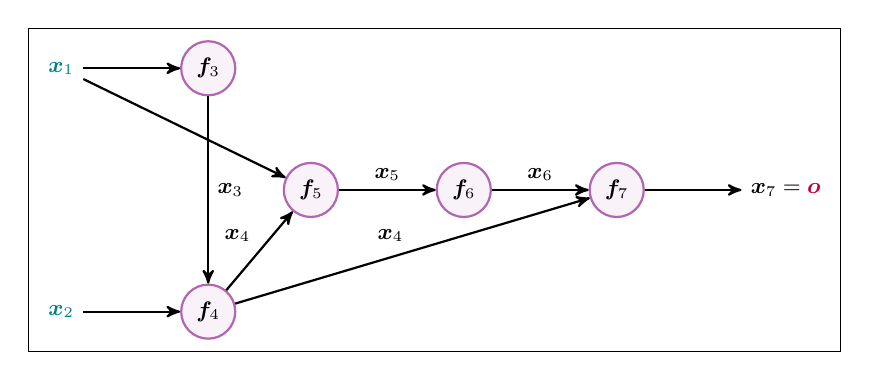
\begin{tikzpicture}[
    roundnode/.style={circle, draw=violet!60, fill=violet!5, minimum size=7mm},
    ->,>=stealth',auto,node distance=3.5em,thick,show background rectangle]
    \tikzstyle{every node}=[font=\small,scale=0.9]
      \node[]
      (anchor0)
      {};
      
      \node[above = of anchor0]
      (input1)
      {\color{teal}$\bm{x}_1$};
      
      \node[below = of anchor0]
      (input2)
      {\color{teal}$\bm{x}_2$};
      
      \node[roundnode, right = of input1]
      (func3)
      {$\bm{f}_3$};

      \node[right = of anchor0]
      (anchor1)
      {};
      
      \node[roundnode, right = of input2]
      (func4)
      {$\bm{f}_4$};
      
      \node[roundnode, right = of anchor1]
      (func5)
      {$\bm{f}_5$};

      \node[roundnode, right = of func5]
      (func6)
      {$\bm{f}_6$};
      
      \node[roundnode, right = of func6]
      (func7)
      {$\bm{f}_7$};

      \node[right = of func7]
      (x7)
      {$\bm{x}_7={\color{purple}\bm{o}}$};
      
      \draw[->] (input1)  --  (func3);
      \draw[->] (input1)  --  (func5);
      \draw[->] (input2)  --  (func4);
      \draw[->] (func3)  --node{$\bm{x}_3$}  (func4);
      \draw[->] (func4)  --node{$\bm{x}_4$}  (func5);
      \draw[->] (func4)  --node{$\bm{x}_4$}  (func7);
      \draw[->] (func5)  --node{$\bm{x}_5$}  (func6);
      \draw[->] (func6)  --node{$\bm{x}_6$}  (func7);
      \draw[->] (func7)  --  (x7);
    \end{tikzpicture}
    \caption{Example for the computation graph of $f(\bm{x}_1,\bm{x}_2)=x_2e^{x_1}\sqrt{x_1+x_2e^{x_1}}$}
    {\footnotesize
    \begin{align*}
        x_3 &=~ f_3(x_1) = e^{x_1} \\
        x_4 &=~ f_4(x_2,x_3) = x_2x_3 \\
        x_5 &=~ f_5(x_1,x_4) = x_1 + x_4 \\
        x_6 &=~ f_6(x_5) = \sqrt{x_5} \\
        x_7 &=~ f_7(x_4,x_6) = x_4x_6
    \end{align*}
    }
    \label{fig:compgraph}
\end{figure}

\begin{figure}[htpb]
    \centering
    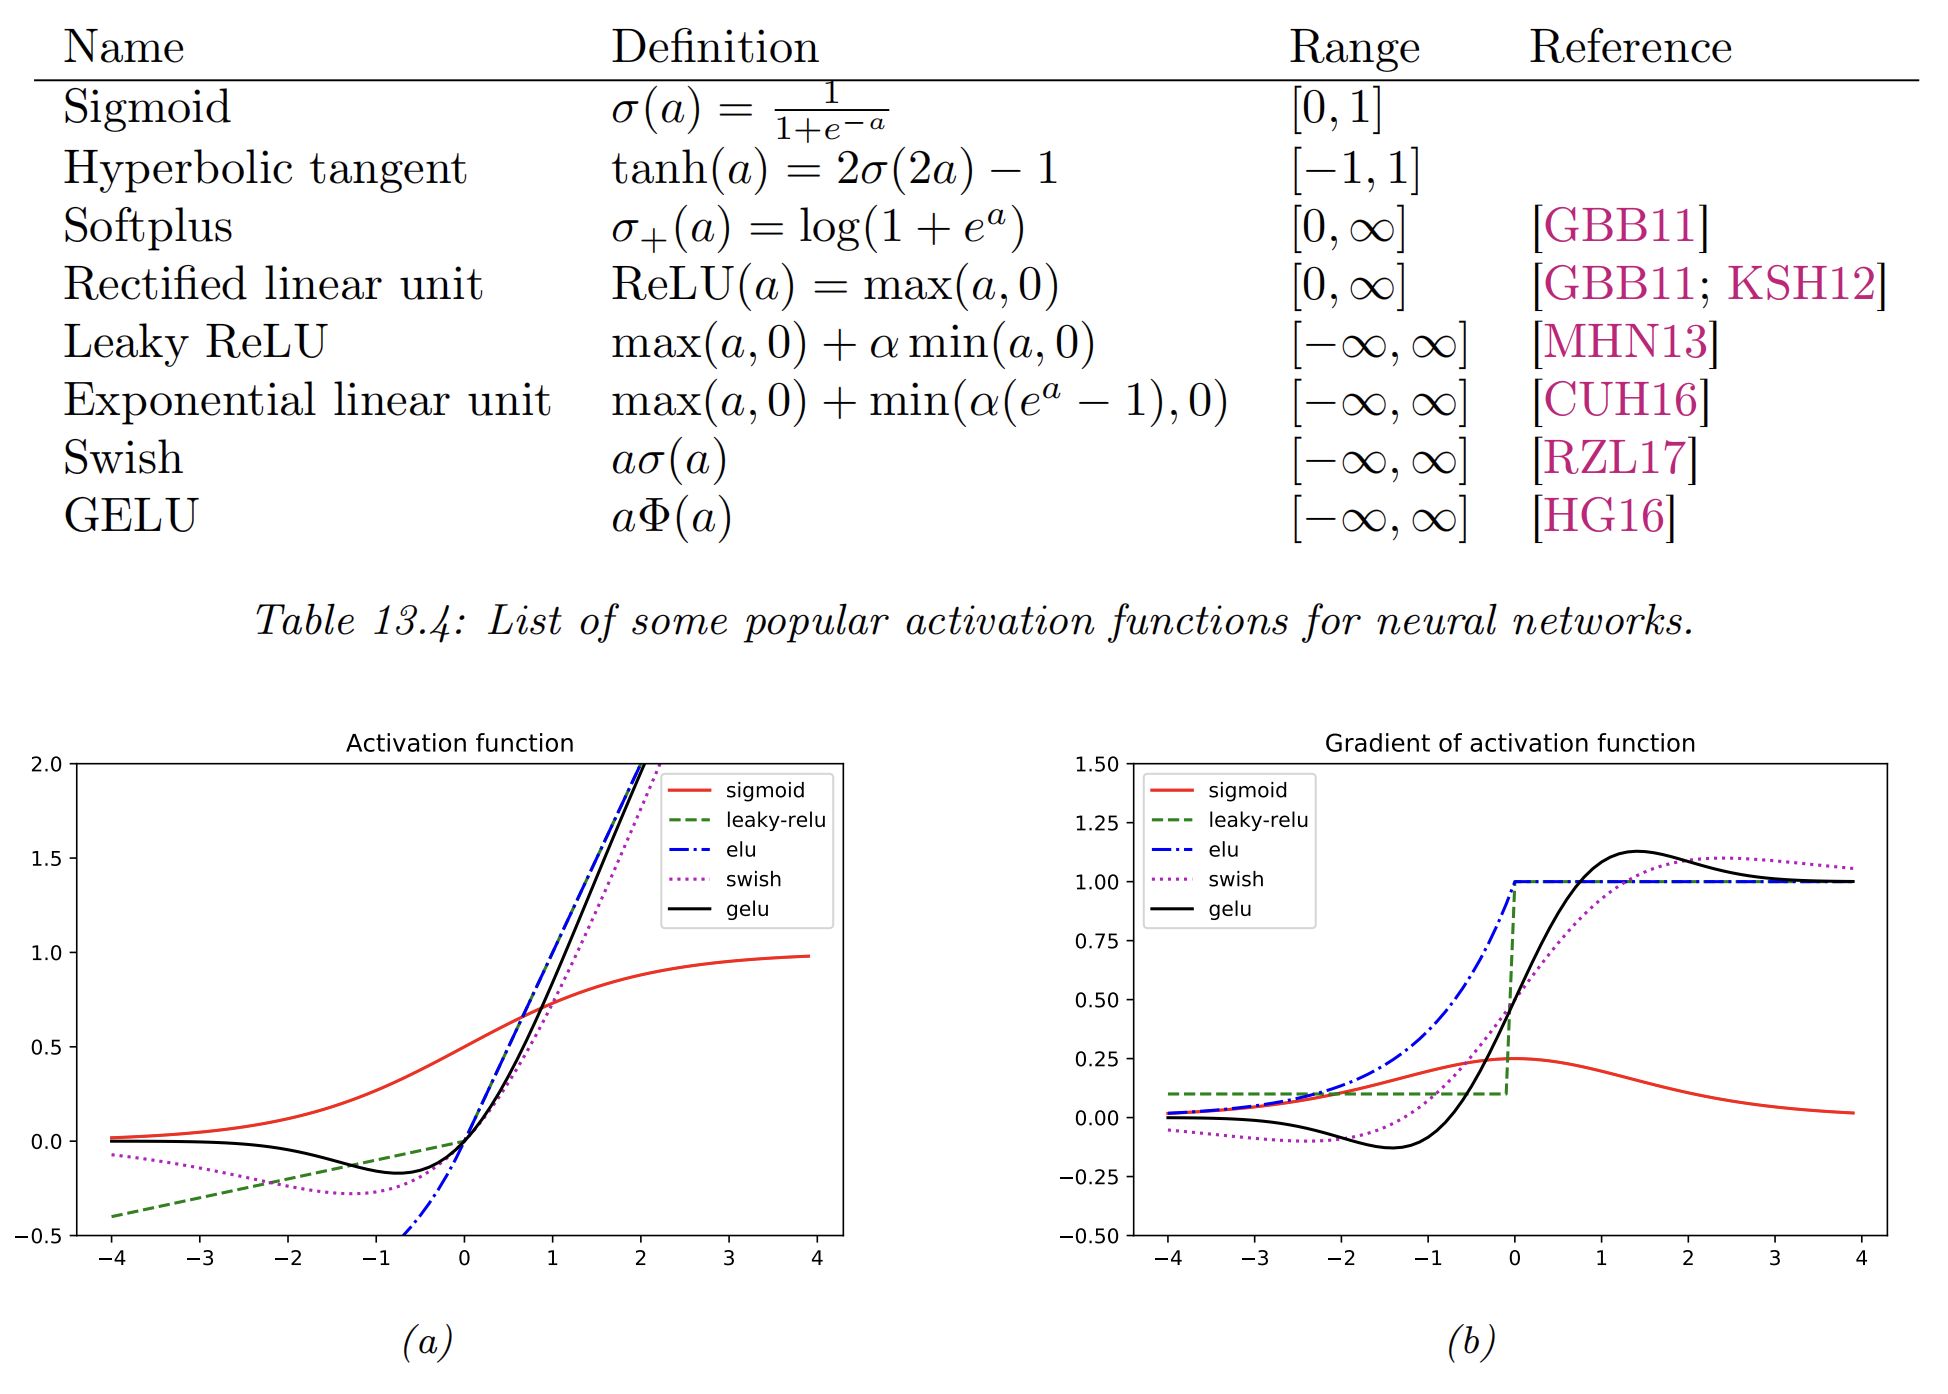
\includegraphics[width=0.75\textwidth]{figs/activationfunc.png}
    \caption{Some popular activation functions and their gradients}
    \label{fig:activationfunc}
\end{figure}

Strategies of solving vanishing gradient problems:
\begin{enumerate}[{(1)}]
    \item modify the activation function to be with proper gradient (e.g \textbf{non-saturating activation functions} in Figure \ref{fig:activationfunc});
    \item modify the architecture to addtively rather than multiplicatively update;
    \item modify the architecture to standardize the activations at each layers (e.g. residual connection in architecture explained below);
    \item carefully choose the initial values of the parameters 
    (e.g. for standard ReLU, the gradient will never escape from zero 
    if the initialized weights such that $\mathbf{W}\bm{x}$ is a large negative value, 
    called \textbf{dead ReLU}. 
    This problem is solved by Leaky ReLU that allows small gradient in the region of negatives.).
\end{enumerate}

\textbf{Residual connections}: 
the layer in a \textbf{residual block} only computes the residual term 
that needs to be added to the input $\bm{x}$ to generate the desired output, 
which does not introduce extra parameters but will be more easy to learn/train.\unsure{
NOTE: The residual connection addition is element-wise, and after an input gets through a residual block, its dimension will not be changed.
}
\begin{gather}
    (\bm{x}_{l+1}=)\Tilde{\bm{f}}_l(\bm{x_l};\bm{\theta}_l) = \bm{f}_l(\bm{x_l};\bm{\theta}_l)+\bm{x}_l\\
    \Rightarrow 
    \Tilde{\bm{f}}(\bm{x};\bm{\theta}_{1:L}) 
    = \Tilde{\bm{f}}_L(\cdots\Tilde{\bm{f}}_l(\bm{x}_l;\bm{\theta}_l)\cdots,\bm{\theta}_L) 
    = \bm{x}_l + \sum_{i=l}^{L}\bm{f}_i(\bm{x}_i;\bm{\theta}_i) \\
    \Rightarrow
    \frac{\partial\mathcal{L}}{\partial\bm{\theta}_l}
    = \frac{\partial\bm{x}_{l}}{\partial\bm{\theta}_l}
      \frac{\partial\mathcal{L}}{\partial\bm{x}_{L}}
      \frac{\partial\bm{x}_{L}}{\partial\bm{x}_{l}}
    = \frac{\partial\bm{x}_{l}}{\partial\bm{\theta}_l}
      \frac{\partial\mathcal{L}}{\partial\bm{x}_{L}}
      \underbrace{\left(
        1 + \sum_{i=l}^{L-1}\frac{\partial\bm{f}_i(\bm{x}_i;\bm{\theta}_i)}{\partial\bm{x}_l}
      \right)}_{\text{other terms}}
\end{gather}
which shows the gradient at layer $l$ can depend directly on the gradient at layer $L$ 
in a way that is independent of the depth of the network.\unsure{
But I am not very sure what is $\frac{\bm{x}_l}{\bm{\theta}_l}$. 
Is it equal to zero since $\bm{x}_l$ and $\bm{\theta}_l$ act as the inputs at the same time 
for a layers and have nothing to do with each other?}

\begin{figure}[htpb]
    \centering
    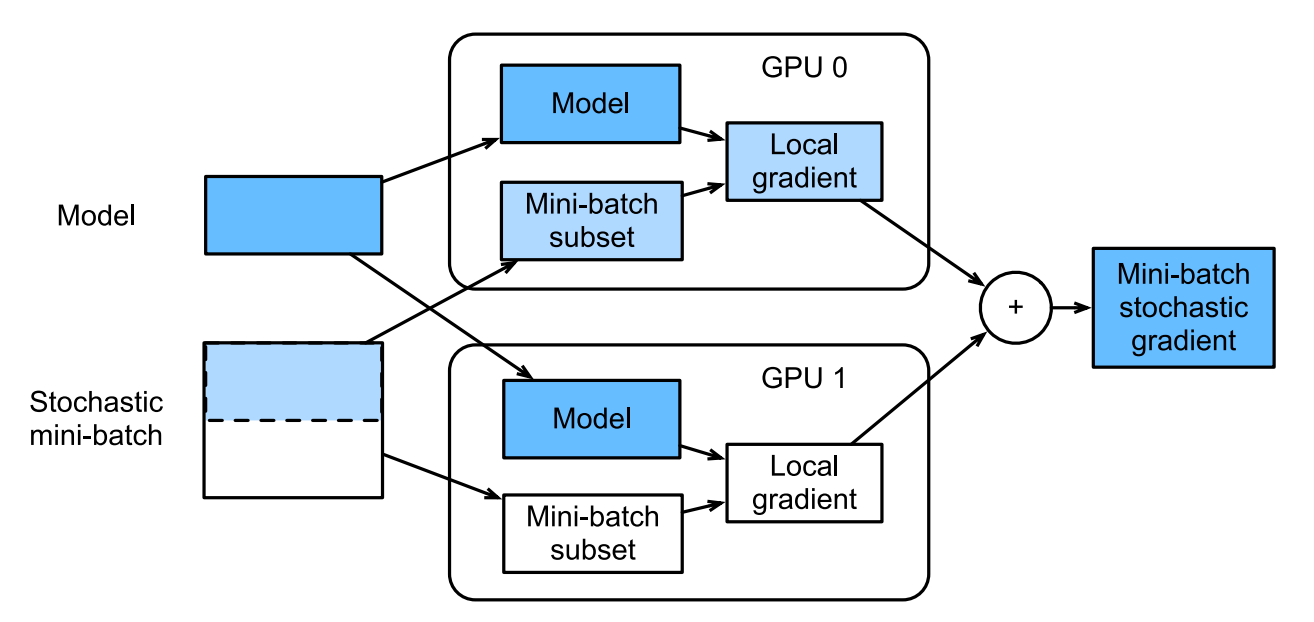
\includegraphics[width=0.75\textwidth]{figs/paralleltrain.png}
    \caption{Parallel training across multiple machines}
    \label{fig:paralleltrain}
    {\footnotesize 
    \textbf{synchronous training}: Each machine \textit{blocks} until receiving the centrally aggregated gradient $\bm{g}_t$, 
    $\Tilde{\bm{g}}_t^k\leftarrow\sum_{k=1}^K\bm{g}_t^k$, 
    and $\bm{\theta}_t^k\leftarrow\bm{\theta}_t^k-\eta_t\Tilde{\bm{g}}_t^k$.
    
    Otherwise, \textbf{asynchronous training}, no aggregation of $\bm{g}_t$ 
    but $\bm{\theta}_t^k\leftarrow\bm{\theta}_t^k-\eta_t\bm{g}_t^k$}
\end{figure}

Other kinds of feedforward networks:
\begin{enumerate}[{(1)}]
    \item 
    \textbf{Radial basis function (RBF) network}: 
    Given a set of $K$ \textit{centroids} or \textit{exemplars}, $\bm{\mu}_k\in\mathcal{X}$\unsure{
    compute the RBF similarity between data points and these outstanding exemplars.
    }
    \begin{gather}
        \phi(\bm{x}) 
        = \left[\mathcal{K}(\bm{x},\bm{\mu}_i)\right]:\mathbb{R}^D\to\mathbb{R}^{K}\\
        \mathcal{K}_\text{gauss}(\bm{x},\bm{c})
        \triangleq \exp\left(-\frac{1}{2\sigma^2}\|\bm{x}-\bm{c}\|_2^2\right) \\
        \begin{cases}
        p(y|\bm{x},\bm{\theta}) = \mathcal{N}(\bm{w}^\mathsf{T}\phi(\bm{x},\sigma^2)) & \text{for regression} \\
        p(y|\bm{x},\bm{\theta}) = \mathrm{Ber}(\sigma(\bm{w}^\mathsf{T}\phi(\bm{x}))) & \text{for classification}
        \end{cases}
    \end{gather}
    \item 
    \textbf{Mixture of linear experts}: a conditional mixture model that regresses multiple outputs that conditioned a certain source, called \textit{expert}\unsure{
    recall the mixture model of Gaussian distributions
    }
    % heteroskedastic regression like Equation (\ref{eq:heteroreg}) will give certain $x$ values two equally probable $y$ values, called \textbf{one-to-many functions}.
    \begin{align}
        p(\bm{y}|\bm{x}) =&~ \sum_{k=1}^K p(\bm{y}|\bm{x},z=k)p(z=k|\bm{x}) \\
        p(\bm{y}|\bm{x},z=k) =&~ \mathcal{N}(\bm{y}|f_{\mu,k}(\bm{x}),\mathrm{diag}(f_{\sigma,k}(\bm{x}))) \\
        p(z=k|\bm{x}) =&~ \mathrm{Cat}(z|\mathrm{softmax}(f_z(\bm{x})))
    \end{align}
\end{enumerate}







% \begin{framed}{\large
% TODO list of the following week
% \begin{itemize}
%     \item Read Chapters 14 \& 15 Neural Network for Image and Sequence Data;
% \end{itemize}
% }
% \end{framed}

% ############################### WK 10 #######################################

% \setcounter{section}{4}
% \setcounter{subsection}{1}
% \begin{center}
% \textit{Chapters 14 \& 15 Neural Network for Image Data \& Sequence Data}
% \end{center}

% \begin{table}[htpb]
    \centering
    \caption{Some short unfamiliar terminologies in Neural Network}
    {\footnotesize

}
    {\small
    \begin{tabular}{cp{32em}}
        \toprule
        Terminology & Explanations \\
        \midrule
        \makecell{\textbf{i\&o size of conv.} \\ {\color{blue}$[x_w,x_h]\to[x'_w,x'_h]$}} &
        $\begin{array}{rl}
            \left[x_h,~x_w\right] 
            \xrightarrow[\text{pad.}]{[p_h,~p_w]} &
            \left[x_h+2p_h,~x_w+2p_w\right] \\ 
            \xrightarrow[\text{$[s_w,~s_h]$ strided conv.}]{[f_h,~f_w]} &
            \left[\lfloor x_h+2p_h-f_h+1\rfloor,~\lfloor x_w+2p_w-f_w+1\rfloor\right]
        \end{array}$ \\
        \makecell{\textbf{multiple i\&o channels} \\ {\color{blue}$[x_w,x_h,C]\to[x'_w,x'_h,D]$}} &
        $z_{i,j,d}=b_d+\sum_{u=0}^{H-1}\sum_{v=0}^{W-1}\sum_{c=0}^{C-1} x_{\color{red}(si+u),(sj+v),c} w_{u,v,c,d}$, 
        there are a of output channels-number ($D$) of linear weights volumes with size of $[H,W,C]$.   \\
        \makecell{\textbf{pointwise conv.} \\ {\color{blue}$[x_w,x_h,C]\to[x'_w,x'_h,D]$}} &
        $z_{i,j,d}=b_d+\sum_{c=0}^{C-1}x_{i,j,c} w_{0,0,c,d}$, 
        weightedly combining the features across channels at location $(i,j)$ \\
        \makecell{\textbf{dilated conv.}} & 
        $z_{i,j,d}=b_d+\sum_{u=0}^{H-1}\sum_{v=0}^{W-1}\sum_{c=0}^{C-1}x_{\color{red}(i+ru),(j+rv),c}w_{u,v,c,d}$, 
        where $r$ is the dilation factor. 
        It also called \textbf{conv. with holes}, e.g. $\Tilde{\bm{w}}=[w_1,0,w_2,0,w_3]$ if $r=2$ and in 1D conv.,
        resulting in larger receptive field but no more parameters.\\
        
        \makecell{\textbf{pooling} \\ local: {\color{blue}$[x_w,x_h,C]\to[x'_w,x'_h,C]$} \\ or global: {\color{blue}$[x_w,x_h,C]\to[1,1,D]$}} &
        (local) max/average pooling replaces the weighted combinition of normal conv. to $\max(\cdot)$/average and is performed \textit{in each channel independently};
        global max/average pooling \textit{summarize} each channel of feature map into \textit{a single value}. \\
        \textbf{ResNet} & $\bm{x}_{l+1} = \varphi(\bm{x}_l + \mathcal{F}_l(\bm{x}_l))$,
        \textbf{PreResnet} $\bm{x}_{l+1} = \bm{x}_l + \varphi(\mathcal{F}_l(\bm{x}_l))$  \\
        \textbf{DenseNet} & $\bm{x}_{l+1} = \left[\boxed{\bm{x}},\boxed{f_1(\bm{x})}, \boxed{f_2(\bm{x},f_1(\bm{x}))}, \boxed{f_3(\bm{x},f_1(\bm{x}),f_2(\bm{x},f_1(\bm{x})))},\cdots\right]$ \\
        \makecell{\textbf{Auto-ML} \& \textbf{neural} \\
        \textbf{architecture search (NAS)}} & 
        find architectures minimizing the validation loss by derivative-free blackbox optimization methods, 
        which could include multiple objectives, like accuracy, model size, training/inference speed, etc, at the same time. \\
        \makecell{\textbf{depthwise separable conv.} \\ {\color{blue}$[W,H,C]\to[W',H',C]\to[W',H',D]$}} & 
        $z_{i,j,d}=b_d+w'_{c,d}\sum_{c=0}^{C-1}\left(\sum_{u=0}^{H-1}\sum_{v=0}^{W-1}x_{(i+u),(j+u),c}w_{u,v}\right)$. 
        The separable conv. reduces the number of param. from $H\times W\times C\times D$ to $H\times W + C\times D$. \\
        \textbf{activation maximization} & AM, randomize a input pixels of image such that maximize the average activation of a particular neuron 
        to see what the ``neurons'' are learning (simple edges/blobs $\to$ texture patterns $\to$ object parts $\to$ whole objects) \\
        \textbf{DeepDream} & amplify the features from all layers by optimizing the energy function 
        $\mathcal{L}(\bm{x})=\sum_{l\in \mathcal{L}}\Bar{\phi}_l(\bm{x})$,
        where $\Bar{\phi}_l=\frac{1}{HWC}\sum_{h,w,c}\phi_{l,h,w,c}(\bm{x})$ (feature vector for layer $l$). \\
        \textbf{teaching force} & $p(\bm{w}_{1:T}) = \prod_{t=1}^T p(w_t|\bm{w1:t-1})$, conditioned on \textit{ground truth} label. \\
        \textbf{echo state network} & initiate the $\mathbf{W}_\text{h2h}$ with $\lambda\approx 1$ and fix it, then only update $\mathbf{W}_\text{h2o}$. \\
        \textbf{liquid state machine} & constrain the output of a neuron to take value from $\{0,1\}$ \\
        \textbf{reservoir computing} & the generic term of the above two \\
        \bottomrule
    \end{tabular}}
    \label{tab:nn4imgseq}
\end{table}

% The reason why not apply MLP to images:
% \begin{enumerate}[{(1)}]
%     \item The dimension of inputs may be variant, then the size of $\mathbf{W}$ will be different for every image;
%     \item The dimension of inputs, even though fixed, is usually very large, the the size of $\mathbf{W}$ will also be large ($W\times H\times C\times D$) and hard to learn;
%     \item The model may not exhibit \textbf{translation invariance}, since the weights are not shared across locations
% \end{enumerate}


\subsection{Neural Network for Image Data}

The interpretation of the inner production $\bm{w}^\mathsf{T}\bm{x}$: 
comparing the input $\bm{x}$ to a learned template or pattern $\bm{w}$;
the better the match is, the larger the activation is.\unsure{
This interpretation is consistent with the cross-correlation in digital image analysis,
which is to detect local patches (canditate $\bm{x}$) with similar patterns with the target patch (the weight $\bm{w}$).
The candidates, with the same size of target patch, are all possible croppings of the whole image.
} 

\textbf{Convolution} for 2D image, also called \textbf{template matching}, is a form of feature detection, 
and the detected features are called \textbf{feature map} ($\mathbf{Y}$)
\begin{align}
    \mathbf{Y}_{i,j}
    = [\mathbf{W}*\mathbf{X}]_{i,j}
    = \sum_{u=0}^{H-1}\sum_{v=0}^{W-1}w_{u,v}x_{i+u,j+v}
\end{align}

\textbf{Transposed conv.} converts a smaller feature map to a larger one weighted by the kernel.
It comes from the matrix multiplication form of normal conv.:
if $\mathbf{W}$ is derived from the kernel $\mathbf{K}$ by the process in example below,
then 
\begin{gather}
    \mathbf{Y}=\text{transConv}(\mathbf{X},\mathbf{K})\iff\bm{y}=\mathbf{W}^\mathsf{{\color{red}T}}\bm{x}
\end{gather}
It is worth noting that \textbf{Deconv.}, distinct with transposed conv., is the inverse operation of conv., 
which recover the original input with a known filter.



\begin{example}\label{ex:convTconv}
    \textbf{Convolution in matrix multiplication form} \& \textbf{Transposed convolution}
    
    All linear operation can be represented as matrix multiplication form.
    The CNNs can be regarded as a 
    {\begin{align}
        \mathbf{Y}
        =&~ \mathbf{K}*\mathbf{X}~~(\text{from big $\mathbf{X}$ to small $\mathbf{Y}$}) \\
        =&~ \left[\begin{array}{cc}
            {\color{red}k_1}   & {\color{blue}k_2} \\
            {\color{green}k_3} & {\color{violet}k_4}
        \end{array}\right]*\left[\begin{array}{ccc}
            x_1 & x_2 & x_3 \\
            x_4 & x_5 & x_6 \\
            x_7 & x_8 & x_9
        \end{array}\right] \\
        =&~ \left[\begin{array}{cc}
            k_1x_1 + k_2x_2 + k_3x_3 + k_4x_4 & 
            k_1x_2 + k_2x_3 + k_3x_5 + k_4x_6 \\
            k_1x_4 + k_2x_5 + k_3x_7 + k_4x_8 & 
            k_1x_5 + k_2x_6 + k_3x_8 + k_4x_9
        \end{array}\right] \\
        \iff \notag\\
        \bm{y} 
        =&~ \mathbf{W}\bm{x} \\
        =&~ \left[\begin{array}{ccc|ccc|ccc}
            {\color{red}k_1}     & {\color{blue}k_2}   & 0                   & 
            {\color{green}k_3}   & {\color{violet}k_4} & 0                   & 
            0                    & 0                   & 0                   \\
            0                    & {\color{red}k_1}    & {\color{blue}k_2}   & 
            0                    & {\color{green}k_3}  & {\color{violet}k_4} & 
            0                    & 0                   & 0                   \\
            0                    & 0                   & 0                   & 
            {\color{red}k_1}     & {\color{blue}k_2}   & 0                   & 
            {\color{green}k_3}   & {\color{violet}k_4} & 0                   \\
            0                    & 0                   & 0                   & 
            0                    & {\color{red}k_1}    & {\color{blue}k_2}   & 
            0                    & {\color{green}k_3}  & {\color{violet}k_4} \\
        \end{array}\right]\left[\begin{array}{c}
            x_1 \\ x_2 \\ x_3 \\ x_4 \\ x_5 \\ x_6 \\ x_7 \\ x_8 \\ x_9
        \end{array}\right] \\
        =&~ \left[\begin{array}{c}
            k_1x_1 + k_2x_2 + k_3x_3 + k_4x_4 \\ k_1x_2 + k_2x_3 + k_3x_5 + k_4x_6 \\
            k_1x_4 + k_2x_5 + k_3x_7 + k_4x_8 \\ k_1x_5 + k_2x_6 + k_3x_8 + k_4x_9
        \end{array}\right]
    \end{align}}
    The transposed CNNs can be regarded as 
    \begin{align}
        \mathbf{Y}
        =&~ \mathbf{K}**\mathbf{X}~~(\text{small $\mathbf{X}$ to big $\mathbf{Y}$}) \\
        =&~ \left[\begin{array}{cc}
            {\color{red}k_1}   & {\color{blue}k_2} \\
            {\color{green}k_3} & {\color{violet}k_4}
        \end{array}\right]**\left[\begin{array}{cc}
            x_1 & x_2 \\
            x_3 & x_4 
        \end{array}\right] \\
        =&~ \left[\begin{array}{ccc}
            {\color{red}k_1}x_1                                                                         & 
            {\color{red}k_1}x_2 + {\color{blue}k_2}x_1                                                  & 
            {\color{blue}k_2}x_2                                                                        \\
            {\color{red}k_1}x_3 + {\color{green}k_3}x_1                                                 & 
            {\color{red}k_1}x_4 + {\color{blue}k_2}x_3 + {\color{green}k_3}x_2 + {\color{violet}k_4}x_1 & 
            {\color{blue}k_2}x_4 + {\color{violet}k_4}x_2                                               \\
            {\color{green}k_3}x_3                                                                       & 
            {\color{green}k_3}x_4 + {\color{violet}k_4}x_3                                              & 
            {\color{violet}k_4}x_4                                                                      \\
        \end{array}\right] \\
        \iff \notag\\
        \bm{y} 
        =&~ \mathbf{W}^\mathsf{T}\bm{x} \\
        =&~ \left[\begin{array}{cccc}
            {\color{red}k_1}     & 0                   & 0                   & 0                    \\
            {\color{blue}k_2}    & {\color{red}k_1}    & 0                   & 0                    \\
            0                    & {\color{blue}k_2}   & 0                   & 0                    \\
            {\color{green}k_3}   & 0                   & {\color{red}k_1}    & 0                    \\
            {\color{violet}k_4}  & {\color{green}k_3}  & {\color{blue}k_2}   & {\color{red}k_1}     \\
            0                    & {\color{violet}k_4} & 0                   & {\color{blue}k_2}    \\
            0                    & 0                   & {\color{green}k_3}  & 0                    \\
            0                    & 0                   & {\color{violet}k_4} & {\color{green}k_3}   \\
            0                    & 0                   & 0                   & {\color{violet}k_4}  
        \end{array}\right]\left[\begin{array}{c}
            x_1 \\ x_2 \\ x_3 \\ x_4
        \end{array}\right] 
        = \left[\begin{array}{c}
            {\color{red}k_1}x_1 \\
            {\color{blue}k_2}x_1 + {\color{red}k_1}x_2 \\
            {\color{blue}k_2}x_2 \\
            {\color{green}k_3}x_1 + {\color{red}k_1}x_3 \\
            {\color{violet}k_4}x_1 + {\color{green}k_3}x_2 + {\color{blue}k_2}x_3 + {\color{red}k_1}x_4 \\
            {\color{violet}k_4}x_2 + {\color{blue}k_2}x_4 \\
            {\color{green}k_3}x_3 \\
            {\color{violet}k_4}x_3 + {\color{green}k_3}x_4 \\
            {\color{violet}k_4}x_4
        \end{array}\right]
    \end{align}
    
\end{example}

\begin{table}[htpb]
    \centering
    {\small
    \begin{tabular}{cp{26em}p{8em}}
        \toprule
        tasks & outputs & models \\
        \midrule
        \textbf{image tagging}          & $\mathcal{Y}=\{0,1\}^C$                           & - \\
        \textbf{objective detection}    & a set of bounding boxes with their class labels' probabilities:
        $\bm{f}_{\bm{\theta}}: \mathbb{R}^{H\times W\times K}\to[0,1]^{A\times A}\times\{1,\cdots,C\}^{A\times A}\times \left(A^4\right)^{A\times A}$,
        where $A\times A$ represent the coord. for $A$ \textbf{anchor boxes} & singleshot detector, YOLO \\
        \textbf{instance segmentation}  & 2D shape mask of each object instance in the image with its label & Mask R-CNN \\
        \textbf{semantic segmentation}  & a class label $y_i\in\{1,\cdots,C\}$ for each pixel. The labels could be depth, surface orientation, etc. & U-Net (enc-dec) \\
        \textbf{human pose estimation}  & the locations of a fixed set of skeletal keypoints  & PersonLab, OpenPose \\
        \bottomrule
    \end{tabular}}
    \caption{Other discriminative vision tasks with CNNs}
    \label{tab:vistasks}
\end{table}

\textbf{Normalization layers}: 
\textit{standardize} the statistics of hidden units to remit the problems of \textit{vanishing or exploding gradients}.
\textbf{Batch normalization (BN)}
(i) makes the optimization landscape significant smoother, 
(ii) reduces the sensitivity to the learning rate, and 
(iii) acts like a regularizer and equivalent to a form of approximate Bayesian inference.
\begin{gather}
    \Tilde{\bm{z}}_n=\mathrm{BN}(\bm{z}_n;\bm{\theta})=\bm{\gamma}\odot\hat{\bm{z}}_n+\bm{\beta},~
    \text{where}~\hat{\bm{z}}_n=\frac{\bm{z}_n-\bm{\mu}_\mathcal{B}}{\sqrt{\bm{\sigma}_\mathcal{B}^2+\epsilon}}
\end{gather}
where $\bm{\mu}_\mathcal{B}$ and $\bm{\sigma}_\mathcal{B}^2$ have the same dimension with channels (treat channel independently).
It should be noted that, besides the \uline{learned parameter $\bm{\gamma}$ and $\bm{\beta}$}, 
the whole training set's $\bm{\mu}_{\mathcal{B}_\text{tr}}$ and $\bm{\sigma}_{\mathcal{B}_\text{tr}}^2$ 
are also kept as parameters to standardize the testing sample(s).
When it is combined with a linear layer, called \textbf{fused batchnorm}, the speed can boost:
\begin{gather}
    \bm{\gamma}\odot(\mathbf{XW}+\bm{b}-\bm{\mu})/\bm{\sigma}+\bm{\beta} \iff \mathbf{XW}'+\bm{b}'
\end{gather}
where $\mathbf{W}'=\bm{\gamma}\odot\mathbf{W}/\bm{\sigma}$ and $\bm{b}'=\bm{\gamma}\odot(\bm{b}-\bm{\mu})/\bm{\sigma}+\bm{\beta}$.

\begin{figure}[htpb]
    \centering
    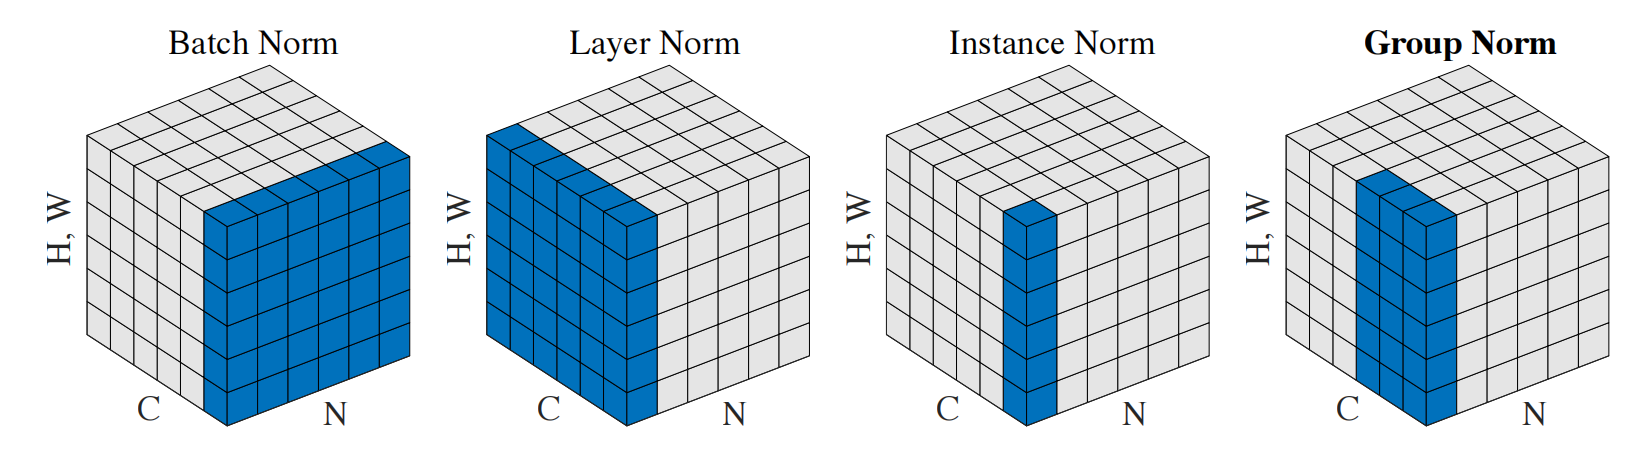
\includegraphics[width=0.8\textwidth]{figs/cnnnormlayer.png}
    \caption{Normalization methods for a CNN}
    {\footnotesize
    \textbf{BN}: pool over height and width in a batch, but match on the channel;
    \textbf{LN}: pool over channel, height and width, but match on the instance index in a batch;
    \textbf{IN}: pool over each instance in the batch and for each channel;
    \textbf{GN}: pool over all locations whose channel is in the same group.
    }
    \label{fig:cnnnormlayer}
\end{figure}

\textbf{Metropolis-adjusted Langevin algorithm (MALA)}: 
sample (generate) images from a generative image model based on trained classifier 
(on current image data), $p(y=c|\bm{x})$, and specified image prior, $p(\bm{x})$,
and under the assumption of normal error\unsure{
{\color{red} This part in \textit{PML: Intro} is in lack of details}
}:
\begin{align}
    p(\bm{x}|y)                     \propto&~     p(\bm{x})p(y|\bm{x}) \\
    \mathcal{E}_c(\bm{x})           \triangleq&~  \log\underbrace{p(y=c|\bm{x})}_\text{trained clf} + \log{\color{teal}p(\bm{x})}~\text{\color{teal}image prior} \\
    \bm{x}'                         =&~           \bm{x} + \frac{\epsilon}{2}\nabla\log{\mathcal{E}_c(\bm{x})} + \mathcal{N}(\mathbf{0},\epsilon\mathbf{I}),~\text{or} \\
    \bm{x}_{t+1}                    =&~           \bm{x}_t 
        + \underbrace{\epsilon_1\nabla_{\bm{x}}\log{p(\bm{x}_t)}}_{\text{plausible under pror}} 
        + \underbrace{\epsilon_2\nabla_{\bm{x}}\log{p(y=c|\bm{x}_t)}}_{\text{plausible under likelihood}} 
        + \underbrace{\mathcal{N}(\mathbf{0},\epsilon_3^2\mathbf{I})}_{\text{intro. randomness}} \label{eq:mala3eps}
\end{align}
\begin{itemize}
    \item \textbf{Gaussian prior}: $p(\bm{x})=\mathcal{N}(\bm{x}|\mathbf{0},\mathbf{I})$, 
    then $\nabla_{\bm{x}}\log{p(\bm{x}_t)}=-\bm{x}_t$ in Equation (\ref{eq:mala3eps});
    \item \textbf{Total variation (TV) prior}: $p(\bm{x})\propto\exp{(-\mathrm{TV}(\bm{x}))}$, 
    where $\mathrm{TV}(\bm{x})$ is \textbf{TV norm}
    \begin{gather}
        \mathrm{TV}(\bm{x})=\sum_{i,j,k}[
            (\underbrace{x_{i,j,k}-x_{(i+1),j,k}}_\text{horizontal Sobel})^2 + 
            (\underbrace{x_{i,j,k}-x_{i,(j+1),k}}_\text{vertical Sobel})^2
        ]
    \end{gather}
\end{itemize}

\textbf{Neural style transfer}: 
generate a new image $\bm{x}$ that re-renders $\bm{x}_c$ in the style of $\bm{x}_s$ 
by optimizing the following energy function
\begin{gather}
    \mathcal{L}(\bm{x}|\bm{x}_s,\bm{x}_c) 
    = \lambda_{\mathrm{TV}}\mathcal{L}_{\mathrm{TV}}(\bm{x}) 
    + \lambda_c\mathcal{L}_{\text{content}}(\bm{x},\bm{x}_c)
    + \lambda_s\mathcal{L}_{\text{style}}(\bm{x},\bm{x}_s) 
\end{gather}
where 
\begin{itemize}
    \item $\mathcal{L}_{\text{content}}$ describes the content similarity between $\bm{x}$ and $\bm{x}_c$ 
    by comparing feature maps of a pre-trained CNN $\phi(\bm{x})$ in the relevant ``content layer'' $l$;
    \begin{gather}
        \mathcal{L}_{\text{content}}(\bm{x},\bm{x}_c)=\frac{1}{C_lH_lW_l}\|\phi_l(\bm{x})-\phi_l(\bm{x}_c)\|_2^2
    \end{gather}
    \item $\mathcal{L}_{\text{style}}$ describes the style similarity between $\bm{x}$ and $\bm{x}_c$
    by interpret visual style as the statistical distribution of certain features that are free from location.
    \begin{align}
        \mathcal{L}_{\text{style}}(\bm{x},\bm{x}_s) =&~
        \sum_{l\in\mathcal{S}}\mathcal{L}_\text{style}^l(\bm{x},\bm{x}_s) \\
        \mathcal{L}_\text{style}^l(\bm{x},\bm{x}_s) =&~
        \|\mathbf{G}_l(\bm{x})-\mathbf{G}_l(\bm{x}_s)\|_F^2 \\
        G_l(\bm{x})_{c,d} =&~ 
        \frac{1}{H_lW_l}\sum_{h=1}^{H_l}\sum_{w=1}^{W_l}\phi_l(\bm{x})_{h,w,c}\phi_l(\bm{x})_{h,w,d}
    \end{align}
\end{itemize}


\subsection{Neural Network for Sequence Data}

\textbf{Forms of RNNs}: transform among embeddings and sequences\unsure{where a initial state $\bm{h}_0$ is assigned in advance.}
\begin{itemize}
    \item sequence generation (\textbf{Vec2Seq}): $f_{\bm{\theta}}:\mathbb{R}^D\to\mathbb{R}^{N_\infty C}$ (from vec $\bm{x}$ to seq $\bm{y}_{1:T}$)
    \begin{align}
        p(\bm{y}_{1:T}|\bm{x}) &=~ \sum_{h_{1:T}}\prod_{t=1}^Tp(\bm{y}_t|\bm{h}_t)p(\bm{h}_t|\bm{h}_{t-1},\bm{y}_{t-1},\bm{x}) \\
        p(\bm{y}_t|\bm{h}_t) &=~ \underbrace{\begin{cases}
        \mathrm{Cat}(\bm{y}_t|\mathrm{softmax}(\mathbf{W}_\text{h2y}\bm{h}_t+\bm{b}_\text{h2y})) ~\text{or}\\
        \mathcal{N}(\bm{y}_t|\mathbf{W}_\text{h2y}\bm{h}_t+\bm{b}_\text{h2y},\sigma^2\mathbf{I})
        \end{cases}}_\text{the only stochasticity}\\
        p(\bm{h}_t|\bm{h}_{t-1},\bm{y}_{t-1},\bm{x}) &=~ \underbrace{\mathbb{I}(\bm{h}_t = f(\bm{h}_{t-1},\bm{y}_{t-1},\bm{x}))}_\text{deterministically computed} \\
        f(\bm{h}_{t-1},\bm{y}_{t-1},\bm{x}) &=~ \varphi(\mathbf{W}_\text{x2h}[\bm{x};\bm{y}_{t-1}]+\mathbf{W}_\text{h2h}\bm{h}_{t-1}+\bm{b}_\text{h}) \label{eq:vec2seqh}
    \end{align}

    \item sequence classification (\textbf{Seq2Vec}): $f_{\bm{\theta}}:\mathbb{R}^{TD}\to\mathbb{R}^{C}$ (from seq $\bm{x}_{1:T}$ to vec $\bm{y}$)
    \begin{align}
        p(y|\bm{x}_{1:T}) 
        =&~ \mathrm{Cat}(y|\mathrm{softmax}(\mathbf{W}\bm{h}^*)) \\
        \bm{h}^*
        =&~ \begin{cases}
            \bm{h}^\rightarrow_T & \text{unidirectional, or} \\
            \Bar{\bm{h}} = \frac{1}{T}\sum_{t=1}^T[\bm{h}^\rightarrow_t,\bm{h}^\leftarrow_t] & \text{bidirectional},~\text{where}
        \end{cases}\\
        % \text{where}~\bm{h}_t 
        % = \varphi(\mathbf{W}_\text{x2h}\bm{x}_{t-1}+\mathbf{W}_\text{h2h}\bm{h}_{t-1}+\bm{b}_\text{h}),\\
        \bm{h}^\rightarrow_t =&~ \varphi(\mathbf{W}^\rightarrow_\text{x2h}\bm{x}_t + \mathbf{W}^\rightarrow_\text{h2h}\bm{h}^\rightarrow_{\color{green}t-1} + \bm{b}^\rightarrow_\text{h}) \label{eq:seq2vech1} \\
        \bm{h}^\leftarrow_t =&~ \varphi(\mathbf{W}^\leftarrow_\text{x2h}\bm{x}_t + \mathbf{W}^\leftarrow_\text{h2h}\bm{h}^\leftarrow_{\color{red}t+1} + \bm{b}^\leftarrow_\text{h}) \label{eq:seq2vech2}
    \end{align}
    
    \item sequence translation (\textbf{Seq2Seq}): $f_{\bm{\theta}}:\mathbb{R}^{TD}\to\mathbb{R}^{T'D}$ (from seq $\bm{x}_{1:T}$ to $\bm{y}_{1:T'}$)\unsure{which can be regarded as labeling every token in a sequence}.
    \begin{align}
        p(\bm{y}_{1:T}|\bm{x}_{1:T'})=&~\begin{cases}
            \sum_{\bm{h}_{1:T}}\prod_{t=1}^T p(\bm{y}_t|\bm{h}_t^L)\mathbb{I}(\bm{h}_t^L 
            = f_L(\bm{h}_{t-1}^L,\bm{x}_t)) & T=T' \\
            f_d(\bm{c})~\text{and}~\bm{c}
            = f_e(\bm{x}_{1:T}) & T \neq T'
        \end{cases} \\
        f_l(\bm{h}_{t-1}^l,\bm{x}_t)
        =&~ \varphi_l(\mathbf{W}_\text{x2h}^l\bm{h}_t^{l-1} + \mathbf{W}_\text{h2h}^l\bm{h}_{t-1}^l + \bm{b}_\text{h}^l) \label{eq:seq2seqh} \\
        p(\bm{y}_t|\bm{h}_t^L)
        =&~ \mathrm{Dist}(\bm{y}_t|\bm{o}_t = \mathbf{W}_\text{h2o}\bm{h}_t^L + \bm{b}_\text{o})
    \end{align}
    where $\bm{c}$ is the context vector encoding the information of input sequence, 
    forming a bottle neck of \textbf{enc-dec architecture}.
\end{itemize}

\textbf{Backpropagation through time}: For the flattened version ${\color{teal}\bm{w}_\text{h}}$ of $[{\color{teal}\mathbf{W}_\text{h2h},\mathbf{W}_\text{h2w}}]$,\unsure{
the expansion is due to the {\color{teal}shared parameters $\bm{w}_\text{h}$ for all $t=0,1,\cdots,T$}
and the {\color{purple}hidden states $\bm{h}_\cdot$, acting as output at current time and input at next time for the same function $f$}.
}
\begin{align}
    \mathcal{L} =&~ \frac{1}{T}\ell{(y_t,\bm{o}_t)} \\
    {\color{purple}\bm{h}_t} =&~ f(\bm{x}_t,{\color{purple}\bm{h}_{t-1}},{\color{teal}\bm{w}_\text{h}}) \\
    \bm{o}_t =&~ g(\bm{h}_t,\bm{w}_\text{o}) \\
    \frac{\partial\mathcal{L}}{\partial{\color{teal}\bm{w}_\text{h}}} 
    =&~ \frac{1}{T}\sum_{t=1}^T
        \frac{\partial\ell(y_t,\bm{o}_t)}{\partial\bm{o}_t}
        \frac{\partial g(\bm{h}_t,\bm{w}_\text{o})}{\partial\bm{h}_t}
        \frac{\partial\bm{h}_t}{\partial{\color{teal}\bm{w}_\text{h}}} \\
    \frac{\partial\bm{h}_t}{\partial{\color{teal}\bm{w}_\text{h}}}
    =&~ \frac{\partial f(\bm{x}_t,\bm{h}_{t-1},{\color{teal}\bm{w}_\text{h}})}{\partial{\color{teal}\bm{w}_\text{h}}}\\
        &+ \sum_{i=1}^{t-1}
        \underbrace{\left(
            \prod_{j=i+1}^t\frac{\partial f(\bm{x}_j,\bm{h}_{j-1},{\color{teal}\bm{w}_\text{h}})}{\partial\bm{h}_{j-1}}
        \right)}_\text{\makecell{causing vanishing or \\exploding gradient problems}}
        \frac{\partial f(\bm{x}_j,\bm{h}_{i-1},{\color{teal}\bm{w}_\text{h}})}{\partial{\color{teal}\bm{w}_\text{h}}}
\end{align}
which requires $O(T^2)$ time to compute for a entire sequence. 
This problem can be handled by truncating the original long sequence into several subsequences lengthing $K$.\unsure{
which requires $O(TK)$ time. The gradients also propagate within the $K$ steps, may causing a $K$-gram model.
}
The update should be relayed across ordered subsequences but reset across random ones.

\begin{figure}[htpb]
    \centering
    \begin{subfigure}[t]{0.45\textwidth}
    \centering
    \label{fig:gru}
    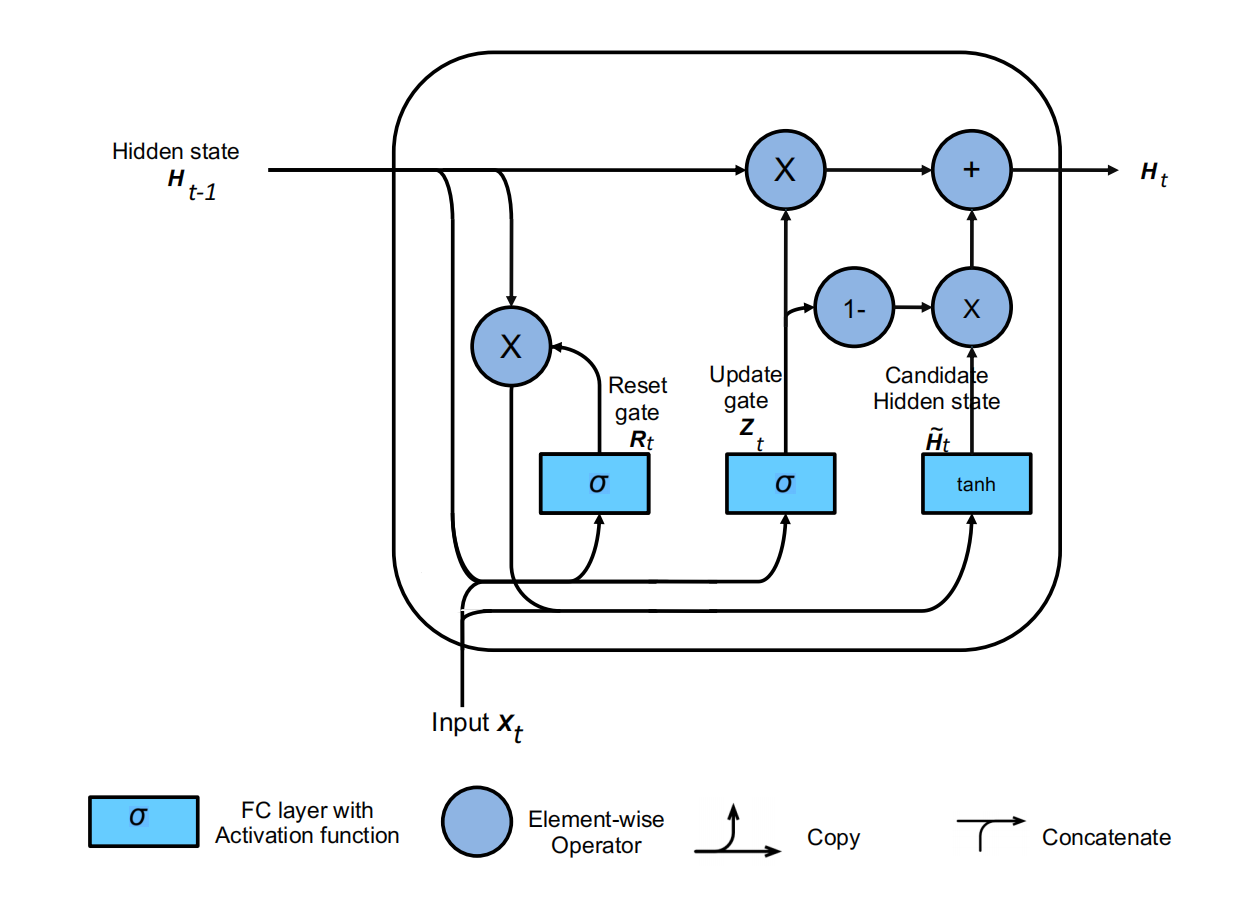
\includegraphics[width=\textwidth]{figs/gru.png}
    \caption{GRU (Gated recurrent units)}
    {\footnotesize
    $\mathbf{H}_t
    = \mathbf{Z}_t\odot\mathbf{H}_{t-1}
    + (1-\mathbf{Z}_t)\odot\Tilde{\mathbf{H}}_t$
    }
    \end{subfigure}
    \begin{subfigure}[t]{0.45\textwidth}
    \centering
    \label{fig:lstm}
    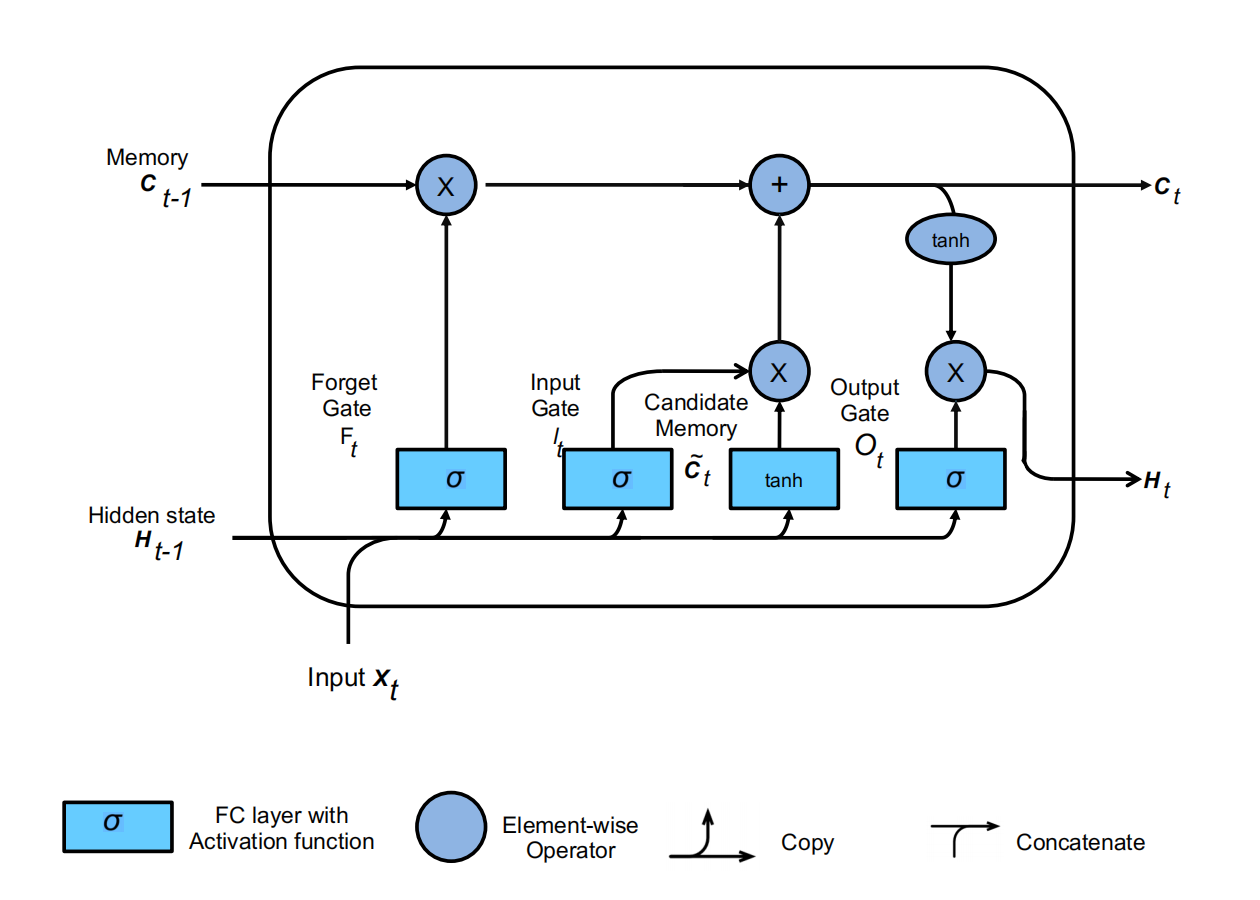
\includegraphics[width=\textwidth]{figs/lstm.png}
    \caption{LSTM (Long short term memory)}
    {\footnotesize
    $\mathbf{C}_t=\mathbf{F}_t\odot\mathbf{C}_{t-1}+\mathbf{I}_t\odot\Tilde{\mathbf{C}}_t$\\
    $\mathbf{H}_t=\mathbf{O}_t\odot\mathrm{tanh}(\mathbf{C}_t)$
    }
    \end{subfigure}
    \caption{Gating and long term momory}
    {\footnotesize
    Since gradient vanishing, the vanilla RNNs fail to remember inputs from long in the past.
    The problem is solved by specify the update of hidden state.
    }
    \label{fig:grulstm}
\end{figure}





\textbf{Beam search}: a heuristic method for decoding a sequence 
by trying top $K$ possible words in each step and record these paths and their probabilities, similar with \textbf{Viterbi algorithm} in decoding a hidden Markov chain.\unsure{
If $K=1$, it gets back to greedy searching that only records the highest possible word in each step, which only achieve a local minimum; 
or if $K=V$, it tries all possibilities and reaches the global optimum but will have $O(V^T)$ complexity of time.
}

\textbf{Causal CNN}, also called \textbf{convolutional Markov model},
is a generative model\unsure{
Recall the generative classifier in Chapter 9, which regards the output $\bm{y}$ is the model's parameters.
}
based on 1D CNN for sequence data but masked out future inputs,
where each output variable, including hidden states, only depends on \textit{previously} generated variables
\begin{gather}
    p(\bm{y})
    = \prod_{t=1}^T p(y_t|\bm{y}_{1:t-1})
    = \prod_{t=1}^T \mathrm{Cat}(y_t|\mathrm{softmax}(\varphi(\sum_{\tau=1}^{t-k}\bm{w}^\mathsf{T}\bm{y}_{\tau:\tau+k}))).
\end{gather}
The long-range dependencies and high-level relationship can be achieved by deeper model (current output, hidden states, as inputs of the next layer) and dilated convolution, both can extend the receptive field of conv. operations, such as the text2speech synthesis system, \textit{wavenet}.




% \begin{framed}{\large
% TODO list of the following week
% \begin{itemize}
%     \item Finish reading Chapter 15;
%     \item Read Chapter 16 Exemplar-based Methods and a half of Chapter 17 Kernel Methods
% \end{itemize}
% }
% \end{framed}


% ############################### WK 11 #######################################

% \setcounter{section}{4}
% \setcounter{subsection}{3}
% \begin{center}
% \textit{Rest of Ch15 NN4Seq, Ch16 Exemplar-based Methods \& part of Ch17 Kernel Methods}
% \end{center}

% \begin{table}[htpb]
    \centering
    \caption{Some short unfamiliar terminologies in Neural Network}
    {\footnotesize

}
    {\small
    \begin{tabular}{cp{32em}}
        \toprule
        Terminology & Explanations \\
        \midrule
        \textbf{Seq2Vec with attention} & for text classification, attention identifies the relevant parts of the input. \\
        \textbf{self-attention} & $\bm{y}_i=\mathrm{Attn}(\mathbf{W}_q^e\bm{x}_i,(\mathbf{W}_k^e\bm{x}_1,\mathbf{W}_v^e\bm{x}_1),\cdots,(\mathbf{W}_k^e\bm{x}_n,\mathbf{W}_v^e\bm{x}_n))$ (encoder) \\
        \textbf{masked attention} & $\bm{y}_i=\mathrm{Attn}(\mathbf{W}_q^d\bm{y}_{i-1},(\mathbf{W}_k^d\bm{y}_1,\mathbf{W}_v^d\bm{y}_1),\cdots,(\mathbf{W}_k^d\bm{y}_{\color{red}i-1},\mathbf{W}_v^d\bm{y}_{\color{red}i-1}))$ (decoder when inference), similar with causal 1D CNN \\
        \textbf{multi-headed attention} & There are a set of $\mathbf{W}_{q_i}$, $\mathbf{W}_{k_i}$, and $\mathbf{W}_{v_i}$ to capture multiple set of features in parallel and \textit{fuse them to a single one} by $\mathbf{W}_o\in\mathbb{R}^{p_o\times hp_v}$.\\
        \textbf{positional encoding} & $\mathbf{X}+\mathbf{P}$, usually use a sinusoidal basis $p_{i,2j}=\sin\left(\frac{i}{C^{2j/d}}\right)$, $p_{i,2j+1}=\cos\left(\frac{i}{C^{2j/d}}\right)$, $i=1:T$ and $d$ is determined by the embedding dimension. PE is similar with binary code of position integers but \textit{more compact}.\\
        \textbf{ViT} & Vision Transformer, split a image to a sequence of $16\times 16$ patches and feed them (prepended a learnable patches, may act as an intercept \uline{representing the whole image like CLS in sequence}) into a transformer encoder for further embedding and classification\\
        \textbf{ELMo} & Embeddings from Language Model, context-specific embedding of each token, $\bm{r}_t^j=\bm{r}_t^\mathsf{T}\bm{w}^j$, 
        where $\bm{r}_t$ is the concatenation of all context and hidden vectors in a RNN model trained in an unsupervised way 
        and $t\to $ lower layer if syntactic task or $t\to$ higher layer if  semantic task \\
        \textbf{masked language model task} &  compute the loss at the masked locations given the others. \\
        \textbf{next sentence prediction task} & For a seq-pair $[\mathrm{CLS}~A_1~A_2\cdots A_m;~\mathrm{SEP}~B_1~B_2\cdots B_n~\mathrm{SEP}]$, 
        $y=1$ if $\mathbf{B}$ is the successor of $\mathbf{A}$ in original text else $y=0$. \\
        \textbf{TL;DR} & ``too long; didn't read'', token telling the model the user wants a summary. \\
        \textbf{T5} & ``Text-to-text Transfer Transformer'', a single model for multiple tasks 
        by telling the system what task to perform as part of the input sentence and then training it as a seq2seq model. \\
        \textbf{C4} & ``Colossal Clean Crawled Corpus'', a 750G corpus of web text for unsupervised training of T5. \\
        \textbf{locality sensitive hashing} & Two data points close in the original space will be close in the projected space by hashing in high probability otherwise in low probability. \\
        \bottomrule
    \end{tabular}}
    \label{tab:nn4imgseq}
\end{table}


\textbf{Attention mechanisms}: 
given $m$ \textbf{key}-\textbf{value} pairs $\{(\bm{k}_i\in\mathbb{R}^k,\bm{v}_i\in\mathbb{R}^v)\}_{i=1}^m$ (examplars) and 
an \textbf{query} $\bm{q}\in\mathbb{R}^q$ as input (new data point), some similarity between the query and keys is calculated 
as  
\begin{enumerate}[{(1)}]
    \item the \textit{weights} that linearly combine the corresponding values (soft attention)\unsure{
    Usually the dimensions of key and query ($k$ and $q$) are the same or mapped to a shared space and 
    $a$ can be any similarity measure $a:\mathbb{R}^{k\times q}\to\mathbb{R}$, 
    including parametric and non-parametric ones, 
    such as kernel functions $a(\bm{q},\bm{k}_i)=\mathcal{K}(\bm{q}-\bm{k}_i)$.
    }
    \begin{gather}
        \mathrm{Atten}(\bm{q},(\bm{k}_{1:m},\bm{v}_{1:m}))
        = \sum_{i=1}^m\alpha_i(\bm{q},\bm{k}_{1:m})=\sum_{i=1}^m\alpha_i(\bm{q},\bm{k}_{1:m})\bm{v}_i\in\mathbb{R}^v \\
        \alpha_i(\bm{q},\bm{k}_{1:m})
        = \mathrm{softmax}_i([{\color{purple}a}(\bm{q},\bm{k}_1),\cdots,{\color{purple}a}(\bm{q},\bm{k}_m)])
    \end{gather}
    \begin{enumerate}
        \item \textbf{additive attention}: 
        $a(\bm{q},\bm{k})=\bm{w}_v^\mathsf{T}\mathrm{tanh}(\mathbf{W}_q\bm{q}+\mathbf{W}_k\bm{k})\in\mathbb{R}$
        \item \textbf{dot-product attention}:\unsure{
        This type of attention is also applied to \textit{self-attention} in Transformer introduced later.
        }
        $a(\bm{q},\bm{k})=\bm{q}^\mathsf{T}\bm{k}/\sqrt{d}\in\mathbb{R}$\unsure{The denominator $\sqrt{q}$  is brought by the assumption of unit variance for $\bm{q}$ and $\bm{k}$.
        }
        \begin{gather}
            \Rightarrow \mathrm{Attn}(\mathbf{Q},]\mathbf{K},\mathbf{V})=\mathrm{softmax}(\frac{\mathbf{QK}^\mathsf{T}}{\sqrt{d}})\mathbf{V}\in\mathbb{R}^{n\times v}
        \end{gather}
    \end{enumerate}
    \item or extract the corresponding value with the \textit{maximal weight} (hard attention)
\end{enumerate}
to form a value fetched by the query.
The attention operation can be parallelized by padding a batch of jagged sequences
and then assigning a large negative value (usually $-10^6$ in practice) to the result of corresponding similarities,
which will generate a tiny weight by softmax to ``mask'' it.\unsure{
This masking mechanism can also be applied to any subset of a sequence, such as the future words after current query.
}

\textbf{Seq2Seq with attention}: allow the output words to directly ``look at'' the input words to avoid bottleneck that limits the information maintaining and to infer the alignment between source and target by calculating a \textit{dynamic context} $\bm{c}_t$ for each word in decoder.
\begin{gather}
    \bm{c}_t=\sum_{i=1}^T\underbrace{\alpha_i(\bm{h}_{t-1}^\mathrm{d},\bm{h}_{1:T}^\mathrm{e})}_{\text{weight},~\in\mathbb{R}}\bm{h}_i^\mathrm{e},\\
    \bm{h}_t^\mathrm{d}=f(\bm{h}_{t-1}^\mathrm{d},[\bm{y}_{t-1},\bm{c}_t])
\end{gather}

\textbf{(Seq+Seq)2Vec}: text pair classification (predicting the relationship between two sentences), 
\begin{enumerate}[{(i)}]
    \item translate seq1 and seq2 to the lengths of each other, 
    \item concatenate and fuse the original sequence features with that of the other's ``shadow'',
    \item pool the words of a fused sentence by summing to form context vector of a seq and its counterpart,
    \item concatenate the two context vectors and classify the relationship.
\end{enumerate}

\begin{figure}[htpb]
    \centering
    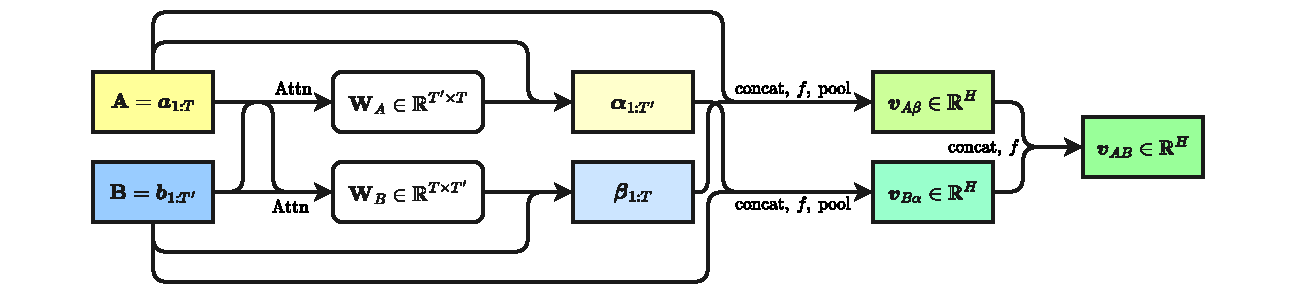
\includegraphics[width=0.9\textwidth]{figs/seqseq2vec.pdf}
    \caption{(Seq+Seq)2Vec}
    \label{fig:seqseq2vec}
\end{figure}


\textbf{Efficient transformers}: 
since the computational complexity of vanilla self-attention model is $O(n^2d)$, 
quadraticly increased with the length of sequence, the modification includes
\begin{enumerate}[{(1)}]
    \item \uline{fixed non-learnable localized attention patterns}: constrain the attention to a fixed non-learnable localized window (block, strided, dilated, or hybrid).
    \item \uline{learnable sparse attention patterns}: partition the long sequence by \textit{(locality sensitive) hashing} (Reformer) or \textit{clustering} (K-means).
    %\unsure{\color{red}I decided to skip it for now, and study it after finish reading this book. it is the famous \textbf{Reformer}'s idea, but I do not understand it yet...}
    \item \uline{memory sharing}: multiple tokens share a side memory module.
    \item \uline{recurrence}: connect different local blocks via recurrence.
    \item \uline{low-rank attention}: approximate attention using low rank matrices.
    \item \uline{kernel methods}: compute attention by kernel function (from low rank matrices), e.g. \textbf{Performer}\unsure{
    This model was considered to reduce PepNN's memory requirement, 
    but that time we did not implement it successfully.
    Its idea involves kernel method, and the details will refer to the following notes of Chapter 17.
    }
\end{enumerate}


\begin{example}
    \textbf{Performer}: Approximate the attention matrices by the kernel of random features

    Before normalization, the attention matrix $\mathbf{A}=[A_{ij}]\in\mathbb{R}^{N\times N}$ can be written as 
    \begin{gather}
        A_{ij}=\exp(\frac{\bm{q}_i^\mathsf{T}\bm{k}_j}{\sqrt{D}})
        = \underbrace{\exp(\frac{-\|\bm{q}_i-\bm{k}_j\|_2^2}{2\sqrt{D}})}_{\color{blue}\mathcal{K}_\text{gauss}(\bm{q}_i/D^{\frac{1}{4}},\bm{k}_j/D^{\frac{1}{4}})}
        \underbrace{\times \exp(\frac{\|\bm{q}_i\|_2^2}{2\sqrt{D}})
        \times \exp(\frac{\|\bm{k}_j\|_2^2}{2\sqrt{D}})}_\text{independent scaling factors}
    \end{gather}
    Moreover, the Gaussian kernel can be written as the expectation of a set of random features, which decouples $\bm{q}$ and $\bm{k}$:
    \begin{gather}
        \mathcal{K}_\text{gauss}(\bm{x},\bm{y})
        = \mathbb{E}\left[\bm{\eta}(\bm{x})^\mathsf{T}\bm{\eta}(\bm{y})\right]
    \end{gather}
    where the $\bm{\eta}(\bm{x})\in\mathbb{R}^M$ is based on trigonometric functions or \uline{exponential functions} 
    (with positive features and better results).
    Then the attention matrix can be rewritten as the following and estimated by a single sample of $\mathbf{Q}'$ and $\mathbf{K}'$
    \begin{gather}
        A_{ij}=\mathbb{E}\left[\bm{\phi}(\bm{q}_i)^\mathsf{T}\bm{\phi}(\bm{k}_j)\right] \\
        \bm{\phi}(\bm{x})\triangleq\exp(\frac{\|\bm{x}\|_2^2}{2\sqrt{D}})\bm{\eta}(\frac{\bm{x}}{D^\frac{1}{4}}) \\
        \Rightarrow
        \mathbf{A}=\mathbb{E}\left[\mathbf{Q}'(\mathbf{K}')^\mathsf{T}\right](\approx\mathbf{Q}'(\mathbf{K}')^\mathsf{T}=:\hat{\mathbf{A}}) \\
        \Rightarrow
        \hat{\mathrm{Attn}}(\mathbf{Q},\mathbf{K},\mathbf{V})=\mathrm{diag}^{-1}(\mathbf{Q}'[(\mathbf{K}')^\mathsf{T}\mathbf{1}_N])(\mathbf{Q}'{\color{blue}[(\mathbf{K}')^\mathsf{T}\mathbf{V}]})
    \end{gather}
    This decoupling of attention matrix enables the parallelization and reduce the memory requirement.
\end{example}

\begin{figure}[htpb]
    \centering
    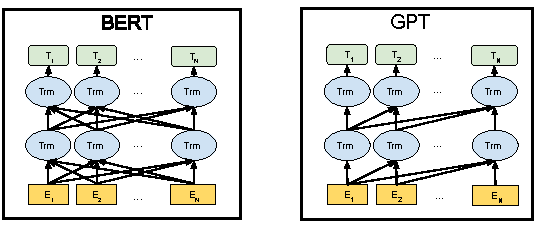
\includegraphics[width=0.8\textwidth]{figs/bertgpt.pdf}
    \caption{BERT \& GPT}
    {\footnotesize
    \textbf{BERT}: Bidirectional Encoder Representations from Transformers, used to create \textit{representations} of text;
    \textbf{GPT}: Generative Pre-training Transformer, used to \textit{generate} text.
    Their difference is whether the training is causal mode.
    }
    \label{fig:bertgpt}
\end{figure}


\section{Nonparametric Models}

\begin{table}[htpb]
    \centering
    \caption{Some short unfamiliar terminologies in Nonparametric Models}
    {\footnotesize

}
    {\small
    \begin{tabular}{cp{32em}}
        \toprule
        Terminology & Explanations \\
        \midrule
        \textbf{exemplar-based models} & \textbf{instance-based learning} and \textbf{memory-based learning}, keeping the training examples around at test times. \\
        \textbf{the curse of dimensionality} & \textit{empty high-dimensional universes that make you feel lonely} \\
        \textbf{k-d tree} & divides space into axis-parallel regions \\
        \textbf{open set recognition} & test samples may come from new categories. \\
        \textbf{online learning} & incremental learning, life-long learning, or continual learning, 
        which often involves \textbf{novelty detection} and encounters \textbf{out-of-distribution (OOD)} and \textbf{few-shot classification} \\
        \textbf{OOD} & Detecting the new class from some entirely different kind of distribution with the previous ones \\
        \textbf{few-shot classification} & only get a few (sometimes just one) example of each class \\
        \textbf{deep metric learning} & learning an embedding of original features $\bm{x}$ by \textit{deep learning models} and computing distances in the embedding space.\\
        \textbf{spherical embedding constraint} & an batchwise regularization term, encouraging all the examples to have the same norm, like Equation (\ref{eq:sec}) \\
        \textbf{stationary kernels} &  kernels whose value only depends on the elementwise difference between the inputs, i.e. $\mathcal{K}(\bm{x},\bm{x}')=\mathcal{K}(\|\bm{x}-\bm{x}'\|)$.
        Instead, \textbf{non-stationary kernel} functions cannot be expressed as simply a function of the distance between their inputs, $\bm{x}-\bm{x}'$.\\
        \textbf{Ornstein-Uhlenbeck process} & $\nu=\frac{1}{2}$ in Matern kernel (Equation (\ref{eq:maternk})), 
        continuous but not differentiable, and hence very ``jagged'', describing the \textit{velocity of a particle undergoing Brownian motion}. \\
        \bottomrule
    \end{tabular}}
    \label{tab:nonparam}
\end{table}




\subsection{Exemplar-based Methods}

\textbf{KNN}: A new nput's label distribution is decided by its $K$ nearest neighbors defined by \textit{Mahalanobis distance}.\unsure{
{\color{red}(How to define the covariance matrix $\mathbf{M}$ given the new input?)} 
This is a topic, \textbf{learning distance metrics}, worth discussed below.
}
\begin{gather}
    p(y=c|\bm{x},\mathcal{D})=\frac{1}{K}\sum_{n\in\mathsf{N}_K(\bm{x},\mathcal{D})} \mathbb{I}(y_n=c) \label{eq:knn} \\
    d_\mathbf{M}(\bm{x},\bm{\mu})=\sqrt{(\bm{x}-\bm{\mu})^\mathsf{T}\mathbf{M}(\bm{x}-\bm{\mu})}.
\end{gather}
Searching the nearest neighbors is the bottleneck of speed and memory requirement, thus the approximation methods are adopted. 
Package \texttt{FAISS} collects a lot of ones.

The methods to \textit{learn} the mahalanobis matrix $\mathbf{M}$ or 
\uline{a linear mapping $\mathbf{W}$ such that $\mathbf{M}=\mathbf{W}^\mathsf{T}\mathbf{W}$}:
\begin{enumerate}[{(1)}]
    \item \textbf{large margin nearest neighbor} (LMNN): in the training process, minimize the distances with the target neighbors with the same class label 
    (\textit{pull} the kindred to neighborhood), 
    and ensure the points with different class labels are more far away than any target neighbors 
    (\textit{push} away the imposters to a further place than the kindred)
    \begin{align}
        \mathcal{L}_\text{pull}(\mathbf{M})
        =&~ \sum_{i=1}^N\sum_{j\in\mathcal{N}_i}d_\mathbf{M}(\bm{x}_i,\bm{x}_j)^2 \\
        \mathcal{L}_\text{push}(\mathbf{M})
        =&~ \sum_{i=1}^N\sum_{j\in\mathcal{N}_i}\sum_{l=1}^N\mathbb{I}(y_i\neq y_l)\left[{\color{blue}m}+d_\mathbf{M}(\bm{x}_i,\bm{x}_j)^2-d_\mathbf{M}(\bm{x}_i,\bm{x}_l)^2\right]_+ \label{eq:lmnnpush} \\
        \mathcal{L}(\mathbf{M}) =&~ (1-\lambda)\mathcal{L}_\text{pull}(\mathbf{M}) + \lambda\mathcal{L}_\text{push}(\mathbf{M}) \\
        \text{or}~\mathcal{L}'(\mathbf{W}) =&~ \mathcal{L}(\mathbf{M}),
    \end{align}
    \item \textbf{neighborhood component analysis} (NCA): 
    maximize the \textit{expected number of correctly classified examples} according for a 1NN classifier by  leave-one-out error.
    \begin{align}
        p_{ij}^\mathbf{W} =&~ \frac{\exp(-\|\mathbf{W}\bm{x}_i-\mathbf{W}\bm{x}_j\|_2^2)}{\sum_{l\neq i}\exp(-\|\mathbf{W}\bm{x}_i-\mathbf{W}\bm{x}_l\|_2^2)} \\
        \mathcal{L}(\mathbf{W}) =&~ 1 - \frac{1}{N}J(\mathbf{W}) = 1 - \frac{1}{N}\sum_{i=1}^N\sum_{j\neq i,y_j=y_i}p_{ij}^\mathbf{W}
    \end{align}
    \item \textbf{latent coincidence analysis} (LCA): maximize the log marginal likelihood of pair's labels $y_n$ 
    by defining the \textit{hierarchical distributions} of \textit{projection} (Gaussian) and \textit{pair's labels} (Bernoulli) and \textit{EM optimization}.
    For a pair of points, $\bm{x}$ and $\bm{x}'$, and the pair index $n$,
    \begin{align}
        p(\bm{z}|\bm{x}) =&~ \mathcal{N}(\bm{z}|\mathbf{W}\bm{x},\sigma^2\mathbf{I}) \\
        p(y=1|\bm{z},\bm{z}') =&~ \exp(-\frac{1}{2\kappa^2}\|\bm{z}-\bm{z}'\|) \\
        \ell(\mathbf{W}, \sigma^2, \kappa^2) =&~ \sum_{n}\log{p(y_n|\bm{x}_n,\bm{x}_n')}
    \end{align}
    \item \textbf{deep metric learning} (DML): learn the distance directly by learning an embedding to a lower dimensional but ``semantic'' space.
    \begin{gather}
        \bm{e} = f(\bm{x};\bm{\theta})\in\mathbb{R}^E,~\hat{\bm{e}} = \frac{\bm{e}}{\|\bm{e}\|_2} \label{eq:sec} \\
        \begin{cases}
        \text{distance} & d(\bm{x}_i,\bm{x}_j;\bm{\theta})^2 = \|\hat{\bm{e}}_i-\hat{\bm{e}}_j\|_2^2 \\
        \text{similarity} & s(\bm{x}_i,\bm{x}_j;\bm{\theta})^2 = \hat{\bm{e}}_i^\mathsf{T}\hat{\bm{e}}_j
        \end{cases}
        {\color{gray}\Rightarrow d^2 = 2-2s^2} \\
    \end{gather}
    \begin{itemize}
        \item \textit{classification losses}: use the loss for classification if the data have label\unsure{
        where the labels act as the indicator of similarity.
        }
        \item \uline{\textbf{ranking loss}}: ensure that similar\unsure{
        The similarity is not necessary to be defined by labels.
        } examples are closer than dissimilar examples:
        \textit{contrastive loss} ($O(N^2)$),\unsure{
        Recall the LMNN's Equation (\ref{eq:lmnnpush})
        } 
        \textit{triplet loss} ($O(N^2)$) and \textit{N-pair loss} ($O(N^3)$)\unsure{
        Note that the $N$ is nothing to do with the total number of instances but pairs used in the loss,
        such as the \textit{hard negatives}.
        }
        {\footnotesize
        \begin{gather}
            \begin{cases}
                \mathcal{L}(\bm{\theta};\bm{x}_i,\bm{x}_j) 
                = \mathbb{I}(y_i=y_j)d(\bm{\bm{x}_i,\bm{x}_j};\bm{\theta})^2
                + \mathbb{I}(y_i\neq y_j)\left[m-d(\bm{x}_i,\bm{x}_j)\right]^2_+ \\
                \mathcal{L}(\bm{\theta};\bm{x}_i,\bm{x}_i^+,\bm{x}_i^-)
                = \left[d(\bm{x}_i,\bm{x}_i^+;\bm{\theta})^2 - d(\bm{x}_i,\bm{x}_i^-;\bm{\theta})^2+m\right]_+ \\
                \mathcal{L}(\bm{\theta};\bm{x},\bm{x}^+,\{\bm{x}_k^-\}_{k=1}^{N-1}) 
                = \log\left(1+\left[\sum_{k=1}^{N-1}\exp(s(\bm{x},\bm{x}_k^-;\bm{\theta}))\right] - s(\bm{x},\bm{x}^+;\bm{\theta})\right)
            \end{cases}
        \end{gather}
        }
    \end{itemize}
\end{enumerate}

The methods to speed up \textbf{ranking loss}'s optimization.
\begin{enumerate}[{(1)}]
    \item \uline{only consider \textit{hard negatives} or up to \textit{semi-hard negatives}}, which requires large batch size and whose set is updated during training. ($O(M^2)$ or $O(M^3)$, $M<N$)
    \item \uline{proxy methods}, measuring the distance between each anchor and \textit{a set of P proxies that represent each class} (updated during training), rather than directly measuring distance between examples. ($O(NP^2)$, $P\sim C<N$)
    \item {\color{gray}\uline{optimize an upper bound} (for the triplet loss) from \textit{triangle inequality} 
    with approximation gap $0\leq\mathcal{L}_t-\mathcal{L}_u\leq\frac{N^3}{C^2}K$, 
    where $K$ depends on the spread of the controids ($O(NC)$):\unsure{
    \color{red}Do not understand this method yet, reread it after finishing the weekly plan...
    }
    {\small\begin{align}
        \|\hat{\bm{e}}_i-\hat{\bm{e}}_j\|-\|\hat{\bm{e}}_i-\hat{\bm{e}}_k\|
        \triangleq&~ \ell_t(\bm{x}_i,\bm{x}_j,\bm{x}_k) \\
        \leq&~ \ell_u(\bm{x}_i,\bm{x}_j,\bm{x}_k) \\
        \triangleq&~ \|\hat{\bm{e}}_i-\bm{c}_{y_i}\|
        -\|\hat{\bm{e}}_i-\bm{c}_{y_k}\|
        +\|\hat{\bm{e}}_j-\bm{c}_{y_i}\|
        +\|\hat{\bm{e}}_j-\bm{c}_{y_k}\|
    \end{align}
    \begin{align}
        &\Rightarrow\sum_{(i,j)\in\mathcal{S},(i,k)\notin\mathcal{S}}\ell_t(\bm{x}_i,\bm{x}_j,\bm{x}_k)
        \triangleq \mathcal{L}_t(\mathcal{D},\mathcal{S}) 
        \leq \mathcal{L}_u(\mathcal{D},\mathcal{S}) \\
        &= \underbrace{3(C-1)(\frac{N}{C}-1)\frac{N}{C}}_{\text{const.}~C'}
        \sum_{i=1}^N\left(
            \|\bm{x}_i-\bm{c}_{y_i}\| - \frac{1}{3(C-1)}\sum_{m=1,m\neq y_i} \|\bm{x}_i-\bm{c}_m\|
        \right)
    \end{align}}}
\end{enumerate}

\textbf{Density kernel}: a function\unsure{
it can measure the similarity by converting from a distance. 
Actually \textit{any integrable function} satisfying 
(i) symmetry about 0, 
{\color{red}(ii) monotone decreasing in $\mathbb{R}^+$ (unimodal on 0)?} 
{\color{blue}It is not necessary, any covariance is possible. See the popular kernels and GP below}, and 
(iii) value $\to 0$ as $x\to\infty$ can serve as a density kernel by normalization.
} satisfying 
\begin{gather}
    \mathcal{K}:\mathbb{R}\to\mathbb{R}^+~\text{such that}~
    \begin{cases}
        \mathcal{K}(x)=\mathcal{K}(-x) & \text{\color{blue}(kernel)} \\
        \int{\mathcal{K}(x)}dx=1 & \text{\color{blue}(density)}
    \end{cases}\\
    \Rightarrow \int{x\mathcal{K}(x-x_n)}dx=x_n
\end{gather}\unsure{
Spread the effect of $x_n$ over the entire space with some covariance.
}
\begin{enumerate}[{(1)}]
    \item \uline{RBF kernel} (Gaussian kernel with bandwidth): $\frac{1}{h}\mathcal{N}(\frac{x}{h}|0,1)$.
    \footnote{To minimize the frequentist risk, set $h = \left(\prod_{d=1}^Dh_d\right)^{\frac{1}{D}}$, 
    where $h_d = \sigma_d\left(\frac{4}{3N}\right)^\frac{1}{5}$, $\hat{\sigma} = 1.4826\mathrm{MAD}$, 
    and $\mathrm{MAD} = \mathrm{median}(|\bm{x}-\mathrm{median}(\bm{x})|)$.}
    \item \uline{boxcar kernel}: $0.5\mathbb{I}(|x|\leq 1)$
    \item \uline{Epanechnikov kernel}: $\frac{3}{4}(1-x^2)\mathbb{I}(|x|\leq 1)$
    \item \uline{tri-{\color{red}cube} kernel}: $\frac{70}{81}(1-|x|^3)^{\color{red}3}\mathbb{I}(|x|\leq 1)$\unsure{
    with finite support and differentiable at supports and the boundaries.
    }
\end{enumerate}


\textbf{Kernel density estimation (KDE)}, a generative model, which defines a probability distribution $p(\bm{x})$
which can be evaluated pointwise and sampled from to generate new data.\unsure{
Recall the Gaussian mixture model with uniform class prior $p(\bm{x}|\bm{\theta})=\frac{1}{K}\sum_{k=1}^K\mathcal{N}(\bm{x}|\bm{\mu}_k,\sigma^2\mathbf{I})$, 
which can regarded as Gaussian kernel density ``estimation'' given $K$ ideal examplars $\bm{\mu}_k$.
}
\begin{gather}
    p(\bm{x}|\mathcal{D}) = \frac{1}{N}\sum_{n=1}^N\mathcal{K}(\bm{x}-\bm{x}_n)
\end{gather}

\textbf{Balloon kernel density estimator}: combine the idea of KNN and KNN, 
specify a dynamic bandwidth for KDE by growing a volume around new input $\bm{x}$ 
until encountering $K$ data points, regardless of their class label.
\begin{gather}
    p(\bm{x}|y=c,\mathcal{D})=\frac{N_c(\mathcal{V}_K(\bm{x}))}{|\mathcal{V}_K(\bm{x})|N_c(\mathcal{V}_\mathcal{D})}
\end{gather}
where $N_c(\mathcal{V})$ the number of examples with label $c$ in volume $\mathcal{V}$, 
$\mathcal{V}_K(\bm{x})$ the volume around $\bm{x}$ embracing $K$ examples, and
$\mathcal{V}_\mathcal{D}$ the entire data space. If the class prior $p(y=c)=\frac{N_c}{N}$,
then Balloon KDE is equivalent to KNN (Equation (\ref{eq:knn})).


\textbf{Kernel regression}:\unsure{
In attention mechanism, the similarity (pre-attention) scores are given by a \textit{non-parametric kernel function} 
and the \textit{values} are the \textit{examplars' labels}
}
In regression problem, do not cast parametric assumption of data distribution but estimate it by KDE, 
then it can show that the prediction is a weighted sum of outputs at the training points, 
where the weights depend on the similarity between the new input $\bm{x}$ and the corresponding training points.
\begin{align}
    \mathbb{E}[y|\bm{x},\mathcal{D}]
    =&~ \int{yp(y|\bm{x},\mathcal{D})}dy=\frac{\int{yp(\bm{x},y|\mathcal{D})}dy}{\int{p(\bm{x},y|\mathcal{D})}dy} \\
    p(\bm{x},y|\mathcal{D})
    \approx&~ \frac{1}{N}\sum_{n=1}^N\mathcal{K}_h(\bm{x}-\bm{x}_n)\mathcal{K}_h(y-y_n) \\
    \Rightarrow \mathbb{E}[y|\bm{x},\mathcal{D}]
    =&~\sum_{n=1}^N y_nw_n(\bm{x})\\
    w_n(\bm{x})
    \triangleq&~ \frac{\mathcal{K}_h(\bm{x}-\bm{x}_n)}{\sum_{n'=1}^N\mathcal{K}_h(\bm{x}-\bm{x}_{n'})}
\end{align}




\subsection{Kernel Methods}


\textbf{Mercer’s theorem}: $\forall$ kernel function $\mathcal{K}$ can be written as $\mathcal{K}(\bm{x},\bm{x}')=\bm{\phi}(\bm{x})^\mathsf{T}\bm{\phi}(\bm{x}')$,
where $\bm{\phi}(\cdot)$ is a feature extraction function that represent the original features $\bm{x}$ into a new feature space.
% (for positive definite matrix $\mathbf{K}$, $K_{ij}=[\mathbf{\Lambda}\frac{1}{2}\mathbf{U}_{:i}]^\mathsf{T}[\mathbf{\Lambda}\frac{1}{2}\mathbf{U}_{:j}]$)

Some popular kernel functions:\unsure{
kernel function describes the distribution of a series r.v. (new inputs) given a observation (anchor for a kernel function).
}
\begin{itemize}
    \item \textbf{automatic relevancy determination (ARD) kernel}: 
    If $d$ is an irrelevant input dimension, we can set $\ell_d = \infty$, 
    so the corresponding dimension will be ignored.
    \begin{gather}
        \mathcal{K}(\bm{r};\bm{\ell},\sigma^2)=\sigma^2\exp\left(
            -\frac{1}{2}\sum_{d=1}^D\frac{1}{\ell_d^2}r_d^2
        \right)
    \end{gather}

    \item \textbf{Matern kernel}: give rise to ``rougher'' functions,\unsure{
    Squared exponential (SE) kernels, $C\exp{(\|\cdot\|_2^2)}$, are infinitely differentiable.
    }
    which can better model local ``wiggles'' without having to make the overall length scale very small.
    \begin{gather}
        \mathcal{K}(r;\nu,\ell)=\frac{2^{1-\mu}}{\Gamma(\mu)}\left(
            \frac{\sqrt{2\mu r}}{\ell}
        \right)^\nu
        \underbrace{K_\nu\left(
            \frac{\sqrt{2\mu r}}{\ell}
        \right)}_\text{Bessel func.}\label{eq:maternk}
    \end{gather}
    
    \item \textbf{periodic kernel} and \textbf{cosine kernel}: capture repeating structure.
    \begin{gather}
        \mathcal{K}(r;\ell,p)=\exp\left(
            -\frac{2}{\ell^2}\sin^2(\pi\frac{r}{p})
        \right) \\
        \mathcal{K}(r;p)=\cos(2\pi\frac{r}{p})
    \end{gather}
    
    \item Old kernels can be \textit{transformed} or \textit{combined} by addition \& multiplication to a new one.
    
    \item \textbf{string kernel}: compare \textit{strings} in terms of the number of n-grams they have in common.
    
    \item \textbf{random walk kernel}: performs random walks on two\textit{graphs} simultaneously, 
    and then counts the number of paths that were produced by both walks.
\end{itemize}





% \begin{framed}{\large
% TODO list of the following week
% \begin{itemize}
%     \item Finish reading Chapter 17 Kernel Methods
%     \item Read Chapter 18 Trees, Forests, Bagging, and Boosting
% \end{itemize}
% }
% \end{framed}

% ############################### WK 11 #######################################

% \setcounter{section}{5}
% \setcounter{subsection}{2}
% \begin{center}
% \textit{Rest of Ch17 Kernel Methods}
% \end{center}

% \textbf{Gaussian process}: define distributions over function of the form $f:\mathcal{X}\to\mathbb{R}$,\unsure{
The function is unknown and non-parametric. The target of GP is to inference the value of function wrt an new input implicitly by defining the relationship between a set of inputs.
}
i.e. giving a distribution for the labels of unlabeled inputs given the observations labeled.
The \textbf{key assumption} is that the function values at a set of $M>0$ inputs,\unsure{
including training set $(\mathbf{X}_{\sim},\bm{y}_{\sim})$ that have observed values of inputs 
and unlabeled but of interest inputs $(\mathbf{X}_*,\bm{Y}_*)$
} 
$\bm{f}(\mathbf{X})=[f(\bm{x}_1),\cdots,f(\bm{x}_M)]$ that can be partitioned to two parts, 
data, $\mathcal{D}=(\mathbf{X}_\dagger,\bm{y}_\dagger)$, and new inputs, $\mathbf{X}_*$ with $\bm{Y}_*\leftarrow\bm{f}(\mathbf{X}_*)$ unknown, WLOG, 
is \uline{jointly Gaussian} with 
mean $\bm{\mu} = [m(\bm{x}_1),\cdots,m(\bm{x}_M)]^\mathsf{T}$ and 
covariance $\mathbf{\Sigma}$ such that $\Sigma_{ij} = \mathcal{K}(\bm{x}_i,\bm{x}_j)$ \unsure{
Recall the {conditionals of an MVN} in Chapter 4.
The conditional distribution of $\bm{Y}_*$ can be inferred given the full distribution of $\bm{Y}=\left[\bm{Y}_\dagger^\mathsf{T},\bm{Y}_*^\mathsf{T}\right]^\mathsf{T}$ and the observation $\bm{Y}_\dagger=\bm{y}_\dagger$.}\unsure{
It is worth noting that every parameter in the density function should \uline{be known} or \uline{be estimated from data}. 
For example, the mean function $m$ is set to be $0$, 
and the kernel function $\mathcal{K}$ is set to be RBF with hyper-parameters $\sigma_f$ and $\ell$:
$\mathcal{K}(\bm{x},\bm{y})=\sigma_f^2\exp(-\frac{1}{2\ell^2}\|\bm{x}-\bm{y}\|_2^2)$.
}
\begin{align}
    \bm{f}(\mathbf{X})
    =&~ \left[\begin{array}{c}
        \bm{f}(\mathbf{X}_\dagger) \\
        \bm{f}(\mathbf{X}_*)
    \end{array}\right]^\mathsf{T} 
    \sim \mathcal{N}{\bm{\mu},\mathbf{\Sigma})} \\
    \bm{\mu} 
    =&~ \left[\begin{array}{c}
        \bm{m}(\mathbf{X}_\dagger) \\
        \bm{m}(\mathbf{X}_*)
    \end{array}\right] \\
    =&: \left[\begin{array}{c}
        \bm{\mu}_\dagger \\
        \bm{\mu}_*
    \end{array}\right] \\
    \mathbf{\Sigma}
    =&~ \mathcal{K}(\mathbf{X}) \\
    =&~ \left[\begin{array}{cc}
        \mathcal{K}(\mathbf{X}_\dagger,\mathbf{X}_\dagger) & \mathcal{K}(\mathbf{X}_\dagger,\mathbf{X}_*) \\
        \mathcal{K}(\mathbf{X}_*,\mathbf{X}_\dagger) & \mathcal{K}(\mathbf{X}_*,\mathbf{X}_*) 
    \end{array}\right] \\
    =&: \left[\begin{array}{cc}
        \mathbf{K}_{\dagger\dagger} & \mathbf{K}_{\dagger*} \\
        \mathbf{K}_{\dagger*}^\mathsf{T} & \mathbf{K}_{**} 
    \end{array}\right]
\end{align}
\begin{gather}
    \Rightarrow 
    \boxed{p(\bm{f}_*)|\mathbf{X}_*,\mathcal{D}) = {\color{red}\textbf{?}}}
\end{gather}
\begin{itemize}
    \item \textbf{noise-free observation}: $y_n=f(\bm{x}_n)$\unsure{
    The computation of posterior distribution involves the inverse operation that may cause \textit{numerical and computational issues}. It can be solved by Cholesky decomposition, i.e. $\mathbf{K}_\sigma=\mathbf{LL}^\mathsf{T}$.
    }
    \begin{align}
        p({\bm{f}}_*|\mathbf{X}_*,\mathcal{D}) 
        =&~ \mathcal{N}({\bm{f}}_*|\Tilde{\bm{\mu}}_*,\Tilde{\bm{\Sigma}}_*) \\
        \Tilde{\bm{\mu}}_*
        =&~ \bm{\mu}_* + \mathbf{K}_{\dagger*}^\mathsf{T}\mathbf{K}_{\dagger\dagger}^{-1}(\bm{f}_\dagger-\bm{\mu}_\dagger) \\
        \Tilde{\bm{\Sigma}}_*
        =&~ \mathbf{K}_{**} - \mathbf{K}_{\dagger*}^\mathsf{T}\mathbf{K}_{\dagger\dagger}^{-1}\mathbf{K}_{\dagger*}
    \end{align}
    \item \textbf{noisy observation}: $y_n=f(\bm{x}_n) + \epsilon_n$, where $\epsilon_n\sim\mathcal{N}(0,\sigma^2)$\unsure{
    The noise is only considered in the observed data (training data), but the prediction process is regarded as noise free.
    }
    \begin{align}
        \mathrm{Cov}(\bm{y}_\dagger|\mathbf{X}_\dagger)
        =&~ \mathbf{K}_{\dagger\dagger}+\sigma^2\mathbf{I}=:\mathbf{K}_\sigma \\
        \left[\begin{array}{c}
            \bm{y}_\dagger \\
            \bm{f}_*
        \end{array}\right]
        =&~\mathcal{N}\left(\left[\begin{array}{c}
            \bm{\mu}_\dagger \\
            \bm{\mu}_*
        \end{array}\right],\left[\begin{array}{cc}
            {\color{red}\mathbf{K}_\sigma} & \mathbf{K}_{\dagger*} \\
            \mathbf{K}_{\dagger*}^\mathsf{T} & {\color{blue}\mathbf{K}_{**}}\label{eq:gpnoisy}
        \end{array}\right]\right)
    \end{align}
\end{itemize}

\textbf{Bayesian linear regression}: linear regression whose weights are r.v.s and 
follow prior distributions, such as \unsure{
BLR needs to work on $\bm{\phi}(\bm{x})$ with finite dimensions explicitly, but GP can work on $\mathbf{K}(=\mathbf{\Phi\Phi}^\mathsf{T})$ implicitly.
}
\begin{align}
    y =&~ f(\bm{x})+\epsilon = \bm{w}^\mathsf{T}\bm{\phi}(\bm{x}) + \epsilon \\
    \epsilon \sim&~ \mathcal{N}(0,\sigma^{-2}) \\
    \bm{w} \sim&~ \mathcal{N}(\bm{0},\bm{\Sigma}_w) \\
    \Rightarrow
    p(\bm{w}|\mathcal{D}) =&~ \mathcal{N}(\bm{w}|\sigma^{-2}\mathbf{A}^{-1}\mathbf{\Phi}^\mathsf{T}\bm{y},\mathbf{A}^{-1}) \\
    \mathbf{\Phi} :=&~ [\bm{\phi}(\bm{x}_1),\cdots,\bm{\phi}(\bm{x}_N)]^\mathsf{T}\in\mathbb{R}^{N\times D} \\
    \mathbf{A} :=&~ \sigma^{-2}\mathbf{\Phi}^\mathsf{T}\mathbf{\Phi} + \mathbf{\Sigma}_w^{-1} \\
    \Rightarrow 
    p(f_*|\bm{x}_*,\mathcal{D})
    =&~ \mathcal{N}(f_*|\sigma^{-2}\bm{\phi}_*^\mathsf{T}\mathbf{A}^{-1}\mathbf{\Phi}^\mathsf{T}\bm{y},\bm{\phi}_*^\mathsf{T}\mathbf{A}^{-1}\bm{\phi}_*)\\
    =&: \mathcal{N}(f_*|\Tilde{{\mu}}_*,\Tilde{{\Sigma}}_*) \\
    \Tilde{{\mu}}_*
    =&~ \bm{\phi}_*^\mathsf{T}\mathbf{\Sigma}_w\mathbf{\Phi}^\mathsf{T}(\mathbf{K}+\sigma^2\mathbf{I})^{-1}\bm{y} \label{eq:blrnote}\\
    =&~ \bm{k}_*^\mathsf{T}\mathbf{K}_\sigma^{-1}\bm{y} \\
    \Tilde{{\Sigma}}_*
    =&~ \bm{\phi}_*^\mathsf{T}\mathbf{\Sigma}_w\bm{\phi}_* - \bm{\phi}_*^\mathsf{T}\mathbf{\Sigma}_w\mathbf{\Phi}^\mathsf{T}(\mathbf{K}+\sigma^2\mathbf{I})^{-1}\mathbf{\Phi}\mathbf{\Sigma}_w\bm{\phi}_*\\
    =&~ k_{**} - \bm{k}_*^\mathsf{T}\mathbf{K}_\sigma^{-1}\bm{k}_*
\end{align}
where $\mathbf{K}=\mathbf{\Phi}\mathbf{\Sigma}_w\mathbf{\Phi}^\mathsf{T}$, $\bm{k}_*=\mathbf{\Phi}\mathbf{\Sigma}_w\bm{\phi}_*$, and ${k}_{**}=\bm{\phi}_*^\mathsf{T}\mathbf{\Sigma}_w\bm{\phi}_*$\unsure{
Note: this model assumes the independency across test samples, 
so the new input $\bm{x}_*$ can be predicted one by one.
}
and Equation (\ref{eq:blrnote}) comes from\unsure{
\color{red}idk how to deduce it...
}
\begin{align}
    \Tilde{{\mu}}_*
    =&~ \sigma^{-2}\bm{\phi}_*^\mathsf{T}\mathbf{A}^{-1}\mathbf{\Phi}^\mathsf{T}\bm{y} \\
    =&~ \sigma^{-2}\bm{\phi}_*^\mathsf{T}\left[
        \sigma^{-2}\mathbf{\Phi}^\mathsf{T}\mathbf{\Phi} + \mathbf{\Sigma}_w^{-1}
    \right]^{-1}\mathbf{\Phi}^\mathsf{T}\bm{y} \\
    =&~ \bm{\phi}_*^\mathsf{T}\mathbf{\Sigma}_w\left[
        \mathbf{\Phi}^\mathsf{T}\mathbf{\Phi}\mathbf{\Sigma}_w + \sigma^{2}\mathbf{I}_D
    \right]^{-1}\mathbf{\Phi}^\mathsf{T}\bm{y} \\
    =&~ \bm{\phi}_*^\mathsf{T}\mathbf{\Sigma}_w\mathbf{\Phi}^\mathsf{T}\left[
        \mathbf{\Phi}\mathbf{\Sigma}_w\mathbf{\Phi}^\mathsf{T} + \sigma^{2}\mathbf{I}_N
    \right]^{-1}\bm{y}~~\text{Lemma \ref{lem:woodburyvar}} \label{eq:lemwoodburyvar}\\
    =&~ \bm{\phi}_*^\mathsf{T}\mathbf{\Sigma}_w\mathbf{\Phi}^\mathsf{T}\left[
        \mathbf{K} + \sigma^2\mathbf{I}_N
    \right]^{-1}\bm{y}
\end{align}
\begin{proof}
    The proof of Step \ref{eq:lemwoodburyvar}
    \begin{align}
        &~{\color{teal}\left[
            \sigma^{2}\mathbf{I}_D + \mathbf{\Phi}^\mathsf{T}\mathbf{\Phi}\mathbf{\Sigma}_w
        \right]^{-1}}\mathbf{\Phi}^\mathsf{T} \\
        =&~ {\color{teal}\sigma^{-2}\mathbf{I}_D - \sigma^{-2}\mathbf{I}_D\mathbf{\Phi}^\mathsf{T}\left[
            \mathbf{I}_D + \mathbf{\Phi}\mathbf{\Sigma}_w\sigma^{-2}\mathbf{I}_D\mathbf{\Phi}^\mathsf{T}
        \right]^{-1}\mathbf{\Phi}\mathbf{\Sigma}_w\sigma^{-2}\mathbf{I}_D} \mathbf{\Phi}^\mathsf{T}\\
        =&~ {\color{teal}\sigma^{-2}\left\{
            \mathbf{I}_D - \mathbf{\Phi}^\mathsf{T}\left[
                \sigma^2\mathbf{I}_N + \mathbf{\Phi}\mathbf{\Sigma}_w\mathbf{\Phi}^\mathsf{T}
            \right]^{-1}\mathbf{\Phi}\mathbf{\Sigma}_w
        \right\}}\mathbf{\Phi}^\mathsf{T}\\
        =&~ \sigma^{-2}\mathbf{\Phi}^\mathsf{T}\left\{
            \mathbf{I}_N - \left[
                \sigma^2\mathbf{I}_N + \mathbf{\Phi}\mathbf{\Sigma}_w\mathbf{\Phi}^\mathsf{T}
            \right]^{-1}\left[
                \mathbf{\Phi}\mathbf{\Sigma}_w\mathbf{\Phi}^\mathsf{T} + \sigma^2\mathbf{I}_N - \sigma^2\mathbf{I}_N
            \right]
        \right\}\\
        =&~ \mathbf{\Phi}^\mathsf{T}\left[
            \sigma^2\mathbf{I}_N + \mathbf{\Phi}\mathbf{\Sigma}_w\mathbf{\Phi}^\mathsf{T}
        \right]^{-1}
    \end{align}
\end{proof}



\begin{lemma}[Matrix inversion lemma]\label{lem:woodbury}
    For $\mathbf{A}\in\mathbb{R}^{n\times n}$, $\mathbf{C}\in\mathbb{R}^{k\times k}$, 
    $\mathbf{U}\in\mathbb{R}^{n\times k}$, and $\mathbf{V}\in\mathbb{R}^{k\times n}$.
    \begin{gather}
        (\mathbf{A}+\mathbf{UCV})^{-1} 
        = \mathbf{A}^{-1} 
        - \mathbf{A}^{-1}\mathbf{U}(
            \mathbf{C}^{-1}
            + \mathbf{VA}^{-1}\mathbf{U}
        )^{-1}\mathbf{VA}^{-1}
    \end{gather}
    \textbf{Woodbury matrix identity} or \textbf{Woodbury formula},
    named after Max A. Woodbury, says that the inverse of a \uline{rank-$k$ correction} of some matrix 
    can be computed by doing a \uline{rank-$k$ correction} to the inverse of the original matrices.\footnote{\hyperlink{https://en.wikipedia.org/wiki/Woodbury_matrix_identity}{https://en.wikipedia.org/wiki/Woodbury\_matrix\_identity}}
\end{lemma}

\begin{lemma}[inverse a correction of matrices]\label{lem:invsum}
    Special case of Lemma \ref{lem:woodbury}
    \begin{align}
        (\mathbf{A} + \mathbf{B})^{-1} 
        =&~ \mathbf{A}^{-1} - \mathbf{A}^{-1}(\mathbf{B}^{-1} + \mathbf{A}^{-1})^{-1}\mathbf{A}^{-1}\\
        =&~ \mathbf{A}^{-1} - \mathbf{A}^{-1}(\mathbf{AB}^{-1} + \mathbf{I})^{-1} \\
        =&~ \mathbf{A}^{-1} - (\mathbf{AB}^{-1}\mathbf{A} + \mathbf{A})^{-1} \\
        (\mathbf{A} - \mathbf{B})^{-1}
        =&~ \mathbf{A}^{-1} + \mathbf{A}^{-1}\mathbf{B}(\mathbf{A} - \mathbf{B})^{-1} \\
        =&~ \sum_{k=0}^\infty (\mathbf{A}^{-1}\mathbf{B})^k\mathbf{A}^{-1}
    \end{align}
\end{lemma}

\begin{lemma}[Binomial inverse theorem]\label{lem:woodburyvar}
    Variants of matrix inversion lemma Lemma \ref{lem:woodbury}. 
    \begin{itemize}
        \item For $\mathbf{A}\in\mathbb{R}^{n\times n}$, $\mathbf{B}\in\mathbb{R}^{k\times k}$, 
        $\mathbf{U}\in\mathbb{R}^{n\times k}$, and $\mathbf{V}\in\mathbb{R}^{k\times n}$.
        \begin{gather}
            (\mathbf{A}+\mathbf{UBV})^{-1} 
            = \mathbf{A}^{-1} 
            - \mathbf{A}^{-1}\mathbf{UB}(
                \mathbf{B}
                + \mathbf{BVA}^{-1}\mathbf{UB}
            )^{-1}\mathbf{BVA}^{-1}
        \end{gather}

        \item For $\mathbf{A}\in\mathbb{R}^{n\times n}$, 
        $\mathbf{B}\in\mathbb{R}^{k\times h}$ (can be any conformable and may be singular), 
        $\mathbf{U}\in\mathbb{R}^{n\times k}$, and $\mathbf{V}\in\mathbb{R}^{h\times n}$.
        \begin{gather}
            (\mathbf{A}+\mathbf{UBV})^{-1} 
            = \mathbf{A}^{-1} 
            - \mathbf{A}^{-1}\mathbf{U}(
                \mathbf{I}
                + \mathbf{BVA}^{-1}\mathbf{U}
            )^{-1}\mathbf{BVA}^{-1}
        \end{gather}
    \end{itemize}
    
    
\end{lemma}

% \unsure{
% \color{red}
% $\bm{v}^\mathsf{T}\mathbf{\Sigma}_1\mathbf{\Sigma}_2\mathbf{A}\bm{u}$
% }
\textbf{Estimating the hyper-parameters of kernel}: besides assigning the kernel directly or 
exhaustively searching the optimum from discrete candidates, 
$\bm{\theta}$ can be optimized by probabilistic perspectives.
\begin{itemize}
    \item \textbf{Empiirical Bayes}: which marginalized out the latent Gaussian vector $\bm{f}(\bm{x})$ in noisy observation and get observation (omitting $\dagger$ symbol and using $\bm{m}(\mathbf{X})=\bm{0}$ mean function here for simplicity) part of Equation (\ref{eq:gpnoisy}), then 
    \begin{align}
        \mathrm{NLL}(\bm{\theta}) 
        =&~ \log p(\bm{y}|\mathbf{X},\bm{\theta})
        = \log \mathcal{N}(\bm{y}|\bm{0},\mathbf{K}_\sigma) \\
        =&~ \frac{1}{2}\bm{y}^\mathsf{T}\mathbf{K}_\sigma^\mathsf{T}\bm{y} - \frac{1}{2}\log|\mathbf{K}_\sigma| - \frac{N_\mathcal{D}}{2}\log(2\pi) \\
        \frac{\partial}{\partial\theta_j}\mathrm{NNL}(\bm{\theta})
        =&~ \frac{1}{2}\mathrm{tr}(
        (\underbrace{\mathbf{K}_\sigma^{-1}\bm{y}}_{\bm{\alpha}}\bm{y}^\mathsf{T}\mathbf{K}_\sigma^{-1}-\mathbf{K}_\sigma^{-1})
        {\color{blue}\frac{\partial}{\partial\theta_j}\mathbf{K}_\sigma}
        )
    \end{align}
    \item \textbf{Bayesian inference}: when available observations are limited, 
    then point estimate of kernel parameters can result poorly,
    so wish to approximate the \uline{posterior distribution over $\bm{\theta}$}.
\end{itemize}

\textbf{GP for classification}: once the likelihood is non-Gaussian, the posterior can not be computed exactly but the kernel parameters $\bm{\theta}$ and latent Gaussian vector $\bm{f}$\unsure{
However, it is not a good choice to model a chance $p\in[0,1]$ using Gaussian r.v..
}
are approximated by \textbf{Hamiltonian Monte Carlo} method 
by computing $\nabla_{\bm{f}}\mathcal{E}(\bm{f},\bm{\theta})$ and $\nabla_{\bm{\theta}}\mathcal{E}(\bm{f},\bm{\theta})$.
\begin{align}
    \mathcal{E}(\bm{f},\bm{\theta})
    =&~ \log p(\bm{y}|\bm{f})p(\bm{f}|\mathbf{X},\bm{\theta}) \\
    =&~ \log \mathcal{N}(\bm{f}|\mathbf{0},\mathbf{K}) + \sum_{n=1}^N \log \mathrm{Ber}(y_n|f_n) + \underbrace{\color{red}\log p(\bm{\theta})}_{?}
\end{align}\unsure{
\color{red}TO BE VERIFIED. This presentation in \cite{pml1Book} may be incorrect. 
\textit{It is not important in our current research though.}
}

\textbf{The advantages and disadvantages of GPs}:
\begin{enumerate}[{(1)}]
    \item [pro] much more flexible
    \item [pro] make fewer priori assumptions beyond smoothness
    \item [pro] well designed to handle the \textit{small sample setting}.
    \item [con] computationally intensive $O(N^3)$
    \begin{enumerate}
        \item \uline{sparse (inducing-point) approximations}: 
        summarize the $N$ training points $\mathbf{X}$ into $M(\ll N)$ inducing points $\mathbf{Z}$, 
        e.g. compressing data \textit{rigorously} using the framework of variational inference;
        \item \uline{exploiting parallelization and kernel matrix structure}: 
        Krylov subspace methods based on matrix vector multiplication, 
        which can be parallelized easily (package \texttt{GPyTorch})
        \item \uline{random feature approximation}: approximate the feature map for many shift invariant kernels using a randomly chosen finite set of $M$ basis functions, reducing the cost to $O(NM+M^3)$. See the below.
    \end{enumerate}
\end{enumerate}

\begin{quote}
    A single, infinitely wide layer of RBF units is equivalent to a GP with an RBF kernel and many kinds of DNNs (in the infinite limit) can be converted to an equivalent GP using a specific kind of kernel known as the neural tangent kernel.
\end{quote}

\begin{lemma}[Random features approximation for RBF kernel]\label{lem:rfarbf}
    For the Gaussian RBF kernel $\mathcal{K}$, one can show that 
    \begin{align}
        \mathcal{K}(\bm{x},\bm{x}')
        \approx&~ \bm{\phi}(\bm{x})^\mathsf{T}\bm{\phi}(\bm{x}'), \\
        \text{where}~\phi(\bm{x})
        \triangleq&~ \frac{1}{\sqrt{T}}\left[
            \sin(\bm{\omega}_1^\mathsf{T}\bm{x}),\cdots,\sin(\bm{\omega}_T^\mathsf{T}\bm{x}),
            \cos(\bm{\omega}_1^\mathsf{T}\bm{x}),\cdots,\cos(\bm{\omega}_T^\mathsf{T}\bm{x})
        \right]\\
        =&~ \frac{1}{\sqrt{T}}\left[
            \sin(\mathbf{\Omega}\bm{x}),\cos(\mathbf{\Omega}\bm{x})
        \right]\label{eq:rff} \\
        \text{or}~\phi(\bm{x})
        \triangleq&~ \frac{1}{\sqrt{M}\exp(\frac{\|\bm{x}\|^2}{2})}\left[
            \exp(\bm{\omega}_1^\mathsf{T}\bm{x}),\cdots,\exp(\bm{\omega}_M^\mathsf{T}\bm{x})
        \right]\label{eq:posfeat}
    \end{align}
    where $T=\frac{1}{2}M$, and $\mathbf{\Omega}\in\mathbb{R}^{T\times D}$ is a \textit{random Gaussian matrix}, 
    $\omega_{ij}\overset{\text{iid}}{\sim}\mathcal{N}(0,\frac{1}{\sigma^2})$. 
    The bias of the approximation \textit{decreases} as $M$ increases. 
    The features in Equation (\ref{eq:rff}) are based on trigonometric, called \textbf{random Fourier features (RFF)}, and those in Equation (\ref{eq:posfeat}) are positive.\footnote{both of which can be \textit{orthogonal or each row} by Gram-Schmidt orthogonalization.}
\end{lemma}

\textbf{Extreme learning machines} applies the Lemma \ref{lem:rfarbf} (Random features approximation) 
to the \textit{kernel in GP} and convert it into a \textit{linear model} of the form
\begin{gather}
    f(\bm{x};\bm{\theta})=\mathbf{W}\bm{\phi}(\bm{x}) = \mathbf{W}h(\mathbf{Z}\bm{x})
\end{gather}
where $h(a)=\frac{1}{\sqrt{M}}[\sin(a),\cos(a)]$ for RBF kernels.
It is equivalent to a one-layer MLP with \textit{random and fixed} input-to-hidden weights.

% \begin{example}[SVM with soft margin]
% $~$
\textbf{SVM with soft margin}\unsure{
SVM for classification is the genuine and original support vector machine.
SVM for regression is a variant of kernel regression with \textbf{epsilon insensitive loss function}, a variant of Huber loss. refer to the kernel bridge regression below.
}
    \begin{enumerate}[(1)]
        \item \textbf{optimal objective}
        \begin{align}
            \min_{\bm{w},w_0,\bm{\xi}}&~\frac{1}{2}\|\bm{w}\|^2+C\sum_{n=1}^{N}\xi_n, \\
            \mathrm{s.t.}&~\xi_n \geq 0,\\
            &~ \Tilde{y}_n(\bm{x}_n^\mathsf{T}\bm{w}+w_0)\geq 1 - \xi_n,
        \end{align}
        
        \item \textbf{Lagrangian}
        {\small\begin{align}
            &~\mathcal{L}(\bm{w},\bm{w}_0,\bm{\alpha},\bm{\xi},\bm{\mu})\\
            =&~ \frac{1}{2}\bm{w}^\mathsf{T}\bm{w} + C\sum_{n=1}^N\xi_n
            - \sum_{n=1}^N\alpha_n[\Tilde{y}_n(\bm{w}^\mathsf{T}\bm{x}_n+w_0)-1+\xi_n]
            -\sum_{n=1}^N\mu_n\xi_n
        \end{align}}
        $\Rightarrow~\hat{\bm{w}}$, $\hat{w}_0$, and $\hat{\bm{\xi}}$ 
        such that $\nabla_{\bm{w}}\mathcal{L}=0$, $\nabla_{w_0}\mathcal{L}=0$, and $\nabla_{\bm{\xi}}\mathcal{L}=0$ 
        and plugin them back into $\mathcal{L}$.
    
        \item \textbf{dual problem}
        \begin{gather}
            L(\bm{\alpha})
            = \sum_{i=1}^N\alpha_i - \frac{1}{2}\sum_{i=1}^N\sum_{j=1}\alpha_i\alpha_j\Tilde{y}_i\Tilde{y}_j\boxed{\bm{x}_i^\mathsf{T}\bm{x}_j}
        \end{gather}
    
        \item \textbf{KKT conditions}
        \begin{gather}
            0 \leq \alpha_n \leq C \\
            \sum_{n=1}^N\alpha_n\Tilde{y}_n = 0
        \end{gather}
        If $\alpha_n=0$, the point is ignored. 
        If $0 < \alpha_n < C$ then $\xi_n=0$, 
        the point lies on the margin. 
        If $\alpha_n = C$, the point can lie inside the margin, 
        and can either be correctly classified if $\xi_n \leq 1$, or misclassified if $\xi_n > 1$. 
        Hence $\sum_{n}\xi_n$ is an upper bound on the number of misclassified points.
        \item \textbf{prediction function}
        \begin{align}
            \hat{y}(\bm{x}) =&~ \mathrm{sign}(f(\bm{x})) \\
            f(\bm{x}) 
            =&~ \hat{w}^\mathsf{T}\bm{x} + \hat{w}_0 \\
            =&~ \sum_{n\in\mathcal{S}}\hat{\alpha}_n\Tilde{y}_n\boxed{\bm{x}_n^\mathsf{T}\bm{x}} 
            + \frac{1}{|\mathcal{S}|}\sum_{i\in\mathcal{S}}\left[
                \Tilde{y}_i - \sum_{j\in\mathcal{S}}\hat{\alpha}_j\Tilde{y}_j\boxed{\bm{x}_j^\mathsf{T}\bm{x}_i}
            \right] \\
            =&~ \sum_{n\in\mathcal{S}}\hat{\alpha}_n\Tilde{y}_n\mathcal{K}(\bm{x}_n,\bm{x}) 
            + \frac{1}{|\mathcal{S}|}\sum_{i\in\mathcal{S}}\left[
                \Tilde{y}_i - \sum_{j\in\mathcal{S}}\hat{\alpha}_j\Tilde{y}_j\mathcal{K}(\bm{x}_j,\bm{x}_i)
            \right]
        \end{align}
        \textbf{Kernel trick} $\mathcal{K}(\bm{x}_n,\bm{x})$ \textit{generalizes} the applications of SVM.
        \item \textbf{probability output}
        \begin{itemize}
            \item \uline{Platt scaling}: regard $f(\bm{x})=\log\frac{p(y=1|\bm{x})}{p(y=0|\bm{x})}$
            \begin{gather}
                p(y=1|\bm{x},\bm{\theta}) = \sigma(af(\bm{x})+b)
            \end{gather}
            \item \uline{RVM, a probabilistic kernel classifier}\unsure{in \cite{pml1Book}, it has the overwhelming performance over L1VM, L2VM, and SVM: sparsest, fastest, probabilistic, multiclass, non-Mercer kernel, EB for optimizing kernel, but non-convex for optimizing $\bm{w}$}: 
            only keep the kernel trick to generate a set of new features
            \begin{gather}
                \phi(\bm{x};\mathbf{X})=\mathcal{K}(\mathbf{X},\bm{x})
            \end{gather}
            of length $N$ and 
            then feed it into a discriminative model with some regularization like $\ell_1$ (L1VM) or empirical Bayes\footnote{automatic relevancy determination, ARD} (relevance vector machine, RVM) for sparse results.
        \end{itemize}
    \end{enumerate}
% \end{example}

\textbf{Kernel bridge regression (KBR)} is equivalent with \textit{bridge regression} that is rewritten by linear kernel form $\mathbf{XX}^\mathsf{T}=:\mathbf{K}$
but the kernel part can be generalized to a wide applications $\mathbf{K}=\mathcal{K}(\mathbf{X},\mathbf{X})$. 
\begin{align}
    f(\bm{x};\bm{w}) 
    =&~ \bm{x}^\mathsf{T}\bm{w} \\
    =&~ \bm{x}^\mathsf{T}\mathbf{X}^\mathsf{T}(\mathbf{XX}^\mathsf{T}+\lambda\mathbf{I}_N)^{-1}\bm{y}\\
    =&~ \mathcal{K}(\mathbf{X},\bm{x})^\mathsf{T}(\mathcal{K}(\mathbf{X},\mathbf{X})+\lambda\mathbf{I}_N)^{-1}\bm{y}
\end{align}

\textbf{SVM for regression} is similar with KBR but with sparse coefficients, allowing to only record a part data for kernel trick by a special loss, \textbf{epsilon insensitive loss},\unsure{
If the predicted value are very close to the observed value, lying inside an $\epsilon$-tube around the prediction, 
the loss of this sample is ignored, i.e. ``throw away'' this data point.
}
whose textbf{optimal objective} is 
\begin{align}
    \min_{\bm{w},w_0}&~\lambda\|\bm{w}\|^2 + \sum_{n=1}^{N_\mathcal{D}}L_{\epsilon}(y_n,\hat{y}_n) \\
    &~\hat{y}_n = \bm{w}^\mathsf{T}\bm{x}_n + w_0 \\
    &~L_{\epsilon}(y_n,\hat{y}_n) \triangleq  
    \begin{cases}
    0                       & |y-\hat{y}| < \epsilon \\
    |y-\hat{y}|-\epsilon    & \text{otherwise}
    \end{cases}
\end{align}
which are equivalent to
\begin{align}
    \min_{\bm{w},w_0,\bm{\xi}^+,\bm{\xi}^-}&~\frac{1}{2}\|\bm{w}\|^2 + C\sum_{n=1}^{N_\mathcal{D}}(\xi^+_n+\xi^-_n) \\
    \mathrm{s.t.}
    &~y_n\leq f(\bm{x}_n) + \epsilon + \xi^+_n \\
    &~y_n\geq f(\bm{x}_n) - \epsilon - \xi^-_n 
\end{align}






% \begin{framed}{\large
% TODO list of the following week
% \begin{itemize}
%     \item Read Chapter 18 Trees, Forests, Bagging, and Boosting \& Chapter 19 Learning with Fewer Labeled Examples
% \end{itemize}
% }
% \end{framed}

% ############################### WK 12 #######################################

% \setcounter{section}{5}
% \setcounter{subsection}{2}
% \begin{center}
% \textit{Chapter 18 Trees, Forests, Bagging, and Boosting and Chapter 19 Learning with Fewer Labeled Examples}
% \end{center}

% \subsection{Trees, Forests, Bagging, and Boosting}

\begin{table}[htpb]
    \centering
    \caption{Some short unfamiliar terminologies in Tree Model}
    {\footnotesize

}
    {\small
    \begin{tabular}{cp{32em}}
        \toprule
        Terminology & Explanations \\
        \midrule
        \textbf{empirical class dist.} & $\hat{\pi}_{ic}={\#\{y_n=c:n\in\mathcal{D}_i\}}/{|\mathcal{D}_i|}$ \\
        \textbf{Gini index} & expected error rate for a node: $G_i=1-\sum_{c=1}^C\hat{\pi}_{ic}^2$ \\
        \textbf{deviance} or entropy & impurity for a node: $H_i=\mathbb{H}(\hat{\bm{\pi}}_i)=-\sum_{c=1}^C\hat{\pi}_{ic}\log\hat{\pi}_{ic}$ \\
        \textbf{surrogate split} & a highly correlated ``backup'' features used when the selected features are miss in some training or testing data. \\
        \textbf{bootstrap sampling} & sample data to the original size with \textit{replacement}, $P(\text{selected})=1-e^{-1}$, with 37\% \textbf{out-of-bag instances (oob)} \\ 
        \textbf{Gradient Boosting} & a generic paradigm of boosting methods, predicts the residual of each step (gradient) with problem specific loss, such as squared loss or regression and binary logloss for classification.\\
        \textbf{Feature importance} & the sum of the gain in accuracy for a certain feature over all non-leaf (internal) nodes \\
        \textbf{Partial dependency plots} & the impact that the most relevant features (a given feature $x_k$ at a single evaluation) have on the output \\
        \bottomrule
    \end{tabular}}
    \label{tab:treemodel}
\end{table}

Decision tree model splits the feature space into multiple region, 
the average label of the samples within which is outputted as prediction. 
The key point is the \textbf{criteria of splitting} given optimal partitioning is a NP-complete problem.
And the tree model have some key pros and cons:
\begin{itemize}
    \item [\texttt{pro}] insensitive to monotone transformations of the inputs since ranking is used for partitioning,
    so need to standardize the data\unsure{
    but the distribution of training and testing data still should be similar or same.
    };
    \item [\texttt{pro}] with automatic variable selection;
    \item [\texttt{pro}] robust to outliers and able to handle missing data.
    \item [\texttt{con}] unable to predict very accurately;
    \item [\texttt{con}] whose structures are unstable which small changes to the inputs can have large effect on 
    due to the hierarchical nature of tree growing process. (\textbf{high variance predictor})
\end{itemize}



\textbf{Ensemble learning} comprehensively integrates the predictions from multiple models
\begin{itemize}
    \item \textit{votting} or committee method: simply average the predictions for regression or take the majority class for classification, with the same bias with the base models but less variance and higher accuracy especially when $M=|\mathcal{M}|$ is large 
    \begin{gather}
        p=P(\sum_{m=1}^M Y_m>\frac{M}{2})=1-F_{\text{binom}(M,\theta)}(\frac{M}{2})
    \end{gather}
    
    \item \textbf{Stacking}, weighted voting, learn the combination weights on a \textit{separate} dataset.\unsure{Comparing with Bayes model averaging: 
    $p(y|\bm{x},\mathcal{D})=\sum_{m\in\mathcal{M}}p(m|\mathcal{D})p(y|\bm{x},m,\mathcal{D})$
    }
    \begin{gather}
        f(y|\bm{x}) = \sum_{m\in\mathcal{M}}w_mf_m(y|\bm{x})
    \end{gather}
    
    \item \textbf{Bagging}, i.e. \textbf{bootstrap aggregating}, train on the selected data 
    and validate on the oob, then (weightedly) average the prediction from models.
    \textbf{Random Forest} is Bagged DT \textit{additionally} based on a randomly chosen subset of features\unsure{
    ``Randomness'' of each tree in the ``forest'' comes from randomly selected samples of bagging and randomly chosen features.
    } to decorrelate the base learners.
    However, bagging only uses 63\% of data for training, which usually damages the performance of DNN.\unsure{
    The base learner can be regarded as \textbf{adaptive basis function} in the linear model.
    }

    \item \textbf{Boosting} sequentially fitting additive models (strong learner): training a base classifier (weak learner) with the \textit{weights of data samples by the errors} made by the previous ones. At each step, the parameters to be optimized include base learner parameters $\bm{\theta}_m$ and the weight of new base learner $\theta_m$ 
    \begin{gather}
        (\bm{\theta}_m.\beta_m)=\argmin_{\bm{\theta}, \beta}\sum_{i=1}^{N}\ell(y_i,f_{m-1}(\bm{x}_i)+\beta F(\bm{x}_i;\bm{\theta}))
    \end{gather}
    \begin{itemize}
        \item \textbf{least squares boosting}: $\ell(y,\hat{y}) = (y-\hat{y})^2$\unsure{
        for regression problem
        }
        \begin{gather}
            \ell(y_i,f_{m-1}(\bm{x}_i)+\beta F(\bm{x}_i;\bm{\theta})) = (r_{im}-\beta F(\bm{x}_i;\bm{\theta}))^2
        \end{gather}

        \item \textbf{exponential loss and AdaBoost}: $\ell(\Tilde{y},\hat{y})=\exp(-\Tilde{y}\hat{y})$\unsure{
        for classification problem. It is also a smooth upper bound on the 0-1 loss. \textbf{\color{red}NOTE} that the exp loss can be written like this only when the label space is $\Tilde{y}\in\{-1,1\}$.
        }\unsure{
        Sensitive to outliers.
        }
        \begin{example}[AdaBoost]
            At step $m$, the optimization objective is 
            \begin{align}
                &~\min_{F,\beta} L_m(F;\beta) \\
                L_m(F,\beta) 
                =&~ \sum_{i=1}^N\exp\left\{
                    -\Tilde{y}_i\left[
                        f_{m-1}(\bm{x}_i) + \beta F(\bm{x}_i)
                    \right]
                \right\} \\
                =&~ \sum_{i=1}^N
                \underbrace{\exp\left\{-\Tilde{y}_if_{m-1}(\bm{x}_i)\right\}}_{\omega_{im}~\text{weight}}
                \exp\left\{
                    -\beta\Tilde{y}_i F(\bm{x}_i)
                \right\} \\
                % \overset{F,\Tilde{y}\in\{-1,1\}}
                {=}&~ (e^\beta - e^{-\beta})\sum_{i=1}^N\omega_{im}\mathbb{I}(\Tilde{y}_i\neq F(\bm{x}_i)) + e^{-\beta}\sum_{i=1}^N\omega_{im} \\
                \Rightarrow
                % \begin{cases}
                F_m =&~ \argmin_{F}\sum_{i=1}^N\omega_{im}\mathbb{I}(\Tilde{y}_i\neq F(\bm{x}_i))\\
                \beta_m =&~ \frac{1}{2}\log\frac{1-\text{err}_m}{\text{err}_m} \\
                % \end{cases}
                \text{where err}_m =&~ \frac{\sum_{i=1}^N\omega_{im}\mathbb{I}(\Tilde{y}_i\neq F_m(\bm{x}_i))}{\sum_{i=1}^N\omega_{im}}
            \end{align}
        \end{example}
        \bigskip
        \item \textbf{log loss and LogitBoost}: $\ell(\Tilde{y},\hat{y})=1/(1+\exp(-2\Tilde{y}\hat{y}))$
        \item $\cdots$
    \end{itemize}
\end{itemize}



% \textbf{Gradient Boosting}: the idea is similar with the above boosting methods but with general losses and solving the $\hat{\bm{f}}=\argmin_{\bm{f}}\mathcal{L}(\bm{f})$ by performing gradient descent in the space of functions

There are a few more improvement in \textbf{XGBoost} compared with normal gradient tree boost:
\begin{enumerate}[(1)]
    \item add regularization term in the loss function,.
    \begin{gather}
        \Omega(f)=\gamma J + \frac{1}{2}\sum_{j=1}^Jw_j^2,
    \end{gather}
    where $J$ is the number of leaves, and the $w_j$ is the leaf's output.
    
    \item apply 2-nd order optimization on the loss,\unsure{
    In the context of regression tree, $F(\bm(x))=w_{q(\bm{x})}$, where $q:\mathbb{R}^D\to \{1,\cdots,J\}$.
    \color{red}However, how to calculate the gradient and hessian of loss wrt the function space of model?
    }
    {\begin{align}
        \mathcal{L}_m(F_m)
        \approx&~ \sum_{i=1}^N\left[
            \ell(y_i,f_{m-1}(\bm{x}_i)) + g_{im}F_m(\bm{x}_i) + \frac{1}{2}h_{im}F_m^2(\bm{x}_i)
        \right] \\
        &~+ \Omega(F_m) + \text{const}
    \end{align}}
    % \begin{gather}
    %     g_{im} = \left.
    %     \frac{\partial \ell(y_i,f(\bm{x}_i))}{\partial f(\bm{x}_i)}
    %     \right|_{f=f_{m-1}},~~
    %     h_{im} = \left.
    %     \frac{\partial^2 \ell(y_i,f(\bm{x}_i))}{\partial f(\bm{x}_i)^2}
    %     \right|_{f=f_{m-1}}
    % \end{gather}
    where 
    $g_{im} = \left.
    \frac{\partial \ell(y_i,f(\bm{x}_i))}{\partial f(\bm{x}_i)}
    \right|_{f=f_{m-1}}$, and 
    $h_{im} = \left.
    \frac{\partial^2 \ell(y_i,f(\bm{x}_i))}{\partial f^2(\bm{x}_i)}
    \right|_{f=f_{m-1}}$.
\end{enumerate}

\section{Beyond Supervised Learning}


\begin{table}[htpb]
    \centering
    \caption{Some short unfamiliar terminologies beyond Supervised Learning}
    {\footnotesize

}
    {\small
    \begin{tabular}{cp{32em}}
        \toprule
        Terminology & Explanations \\
        \midrule
        \textbf{AutoAugment} & Using blackbox optimization methods to learn which augmentations work best. \\
        \textbf{adapters} & keep the pre-trained model untouched, but add new parameters (layers inserted inside of the pre-trained model) to modify its internal behavior to customize the feature extraction process for each task \\
        \textbf{Imputation task} & aka fill-in-the blank task or cloze task (in NLP), $\hat{\bm{x}}_h=f(\bm{x}_v,\bm{x}_h=\mathbf{0})$ \\
        \textbf{proxy task} & aka pretext task, $p(y|\bm{x}_1,\bm{x}_2)=p(y|r(f(\bm{x}_1),f(\bm{x}_2)))$ to predict the relationship (proxy label that we \textit{set}) between $\bm{x}_1$ and $\bm{x}_2$ by a common representation learning \\
        \textbf{\makecell{conditional energy\\based model}} & model with the form $p(\bm{x}_2|\bm{x}_1)={\exp\{-\mathcal{E}(\bm{x}_2|\bm{x}_1)\}}/{Z(\bm{x}_1)}$, $Z(\bm{x})=\int{\exp\{-\mathcal{E}(\bm{y}|\bm{x})\}}d\bm{y}$ (\textbf{partition function}, a normalization constant) \\ 
        \textbf{MoCo} & momentum contrastive learning, when there is no enough diverse negatives in a batch, a memory bank is built for generating new negative embeddings by exponential moving averaging \\
        \textbf{promot engineering} & disambiguating phrases added hand when the raw class names can be ambiguous across/within a dataset \\
        \textbf{domain adaptation} & inputs from different domain (source and target domains), $\mathcal{X}_s\neq\mathcal{X}_t$, but outputs from a common domain, $\mathcal{Y}$, 
        \textit{dual} of \textbf{transfer learning}, which has inputs from a common domain and outputs from different domains. \\
        \textbf{pseudo labeling} & aka self-training, use the predictions from the model itself on unlabeled data (by \textit{offline} or \textit{online}) as ``labels'' for subsequent training. \\
        \textbf{confirmation bias} & the model is continually confirming its own (incorrect) bias about the decision rule if the model generates incorrect predictions for unlabeled data and retrains on them.\\
        \textbf{cluster assumption} & the decision boundary between classes should fall in a low-density region of the data manifold which can be estimated from the unlabeled data and derives \textit{entropy minimization}. \\
        \textbf{manifold assumption} & Two datapoints ``similar'' in some meaningful way are expected to share a label. \\
        \textbf{transductive learning} & learn to predict labels for a \textbf{fixed} unlabeled dataset, rather than learn a model that generalizes labels for any new input, which is called \textbf{inductive learning}. \\
        \textbf{meta learning} & learning the parameters of the estimator itself ($\hat{f}(\bm{x};\bm{\theta}(\mathcal{D}_{j+1};{\color{red}\bm{\phi}(\mathcal{D}_{1:J})}))$, learning to learn). \\
        \textbf{MAML} & model-agnostic meta-learning, $\bm{\phi}^*=\argmax_{\bm{\phi}}\frac{1}{J}\sum_{j=1}^J\log p(\mathcal{D}_\text{val}^j|\hat{\theta}_{j}(\bm{\phi},\mathcal{D}_\text{tr}^j))$, equivalent to an \textit{approximate MAP estimate} using a Gaussian prior centered at $\bm{\phi}$. \\
        \textbf{Few-shot learning} & learn to predict fro very few labeled examples, 
        in \textit{extreme} situations, the ``few'' can reduce to one or zero. \\
        \textbf{C-way N-shot classification} & a common way to evaluate FSL methods, classifying $C$ classes using only $N$ examples for \textit{each} class.\\
        \textbf{Matching networks} & learn a metric measuring the similarity on some \textit{external} dataset, and then compare the new input $\bm{x}$ to all the labeled examples $\bm{x}_n$ in the context. \\
        \textbf{weakly supervised learning} & the labels $y$ in training set are not exact (a general term) for classification. \\
        \textbf{label smoothing} & A distribution, $p(y|\bm{x}_n)$, compared with the original delta function, is applied for each label in the cross entropy loss $\mathcal{L}(\bm{\theta})=-\sum_n\sum_y {\color{blue}p(y|\bm{x}_n)}\log q_{\bm{\theta}}(y|\bm{x}_n)$ \\
        \textbf{multi-instance learning} & only labeling a bag/group of examples \\
        \textbf{distance supervision} & use some known facts to label other unlabled data based on the other data's \textit{semantic relationship} (I guess) with the fact. \\
        \bottomrule
    \end{tabular}}
    \label{tab:fewexamplars}
\end{table}

\subsection{Learning with Fewer Labeled Examples}

\textbf{Theoretical justification} for \textbf{data augmentation}: a way to algorithmically inject prior knowledge
\begin{align}
    &~p_\mathcal{D}(\bm{x},\bm{y}) = \frac{1}{N}\sum_{n=1}^N\delta(\bm{x}-\bm{x}_n)\delta(\bm{y}-\bm{y}_n)\\
    \to
    &~p_\mathcal{D}(\bm{x},\bm{y}|A) = \frac{1}{N}\sum_{n=1}^N p(\bm{x}|\bm{x}_n,A)\delta(\bm{y}-\bm{y}_n)\\
    \text{e.g.}&~~p(\bm{x}|\bm{x}_n,A)=\mathcal{N}(\bm{x}|\bm{x}_n,\sigma^2\mathbf{I})
\end{align}


 \textbf{Contrastive task} creates pairs of examples semantically similar to each other (e.g. using data augmentation methods),
 and then to ensure that the distance between their representations is closer than the distance between unrelated examples. 
 For examples,
\begin{enumerate}[(1)]
    \item \textbf{SimCLR}: \textit{Simple contrastive learning of visual representations},\unsure{
    consistent with the basic concept of contrastive learning
    }
    maximize the similarity (cosine similarity) between the views augmented from the same sample and minimize that between unrelated views from different samples.
    \item \textbf{CLIP}: \textit{Contrastive Language-Image Pre-training}, determine if one strings is more likely to be the correct text paired with the given image than another string,\unsure{
    the idea of contrastivity is similar with SimCLR but the counterparts to paired are image and text, respectively, instead of augmented images from one, 
    so the normalization of embedding is required considering heterogeneous embedding spaces are involved.
    }
    which can be used to \textbf{zero-shot classification}.
\end{enumerate}

\textbf{Domain adversarial learning} minimizes the loss of classifying label $y$ but maximize the loss of classifying the source domain $d$
{\small\begin{gather}
    \min_{\bm{\phi}}\max_{\bm{\theta}} \frac{1}{|\mathcal{D}_s|+|\mathcal{D}_t|} \sum_{n\in\mathcal{D}_s,\mathcal{D}_t}
    \ell(d_n,\bm{f}(\bm{x}_n;\bm{\theta})) + \frac{1}{|\mathcal{D}_s|}\sum_{m\in\mathcal{D}_s}\ell(y_m,g(\bm{f}(\bm{x}_m;\bm{\theta});\bm{\phi})),
\end{gather}}
where $\bm{f}(\cdot;\bm{\theta}):\mathcal{X}_s\cup\mathcal{X}_t\to\mathcal{H}$, and $g(\cdot;\bm{\phi}):\mathcal{H}\to\mathcal{Y}$.
This can be implemented by the \textit{gradient sign reversal} trick.


\textbf{Input-output mutual information}: maximize the mutual information of input and output and can also derive \textit{entropy minimization}\unsure{
Another principle is \textit{cluster assumption}
} 
but under a priori that all classes are equally likely. 
\begin{gather}
    \mathcal{I}(y;\bm{x})=\underbrace{\mathbb{E}_{\bm{x}}\sum_{i=1}^Lp(y_i|\bm{x})\log p(y_i|\bm{x})}_\text{neg. \textit{entropy minimization} obj.}
        -\underbrace{\sum_{i=1}^L\mathbb{E}_{\bm{x}}[p(y_i|\bm{x})\log\mathbb{E}_{\bm{x}}p(y_i|\bm{x})]}_\text{equal class proba. assumption}
\end{gather}

\textbf{Co-Training}, similar to self-training, additionally assumes that there are 
\textit{two complementary} (informative-but-independent) ``views'' of the data, 
both of which can be used separately to train a reasonable model, and for a given new input, 
only high-confident pseudo label is used for retraining.

\textbf{Tri-Training} trains three models based on independently sampled datasets with replacement, 
where the pseudo-labels output agree on two will be feeded to retrain the third, and repreat the process iteratively.

\textbf{Label propagation on graphs}, according to the manifold assumption, propagates the known labels across
edges of the graph in such a way that there is minimal disagreement in the labels of a given node's neighbors
according to the similarity between samples.
\begin{align}
    \mathbf{Y}\leftarrow&~\mathbf{TY}\\
    Y_{ic}\leftarrow&~\frac{Y_{ic}}{\sum_{k}Y_{ik}}
\end{align}
where $\mathbf{T}\in\mathbf{R}^{(M+N)\times(M+N)}$ is transition matrix defined by some measure of similarity between sample $i$ and $j$, $w_{ij}$ that $T_{ij}=\frac{w_{ij}}{\sum_{k}w_{ij}}$, and
$\mathbf{Y}\in\mathbb{R}^{(M+N)\times C}$ is label matrix representing the probability of classes for each sample.

\textbf{Consistency regularization}: the perturbing on a given datapoint should not cause the model's output to change \textbf{dramatically}.
\begin{gather}
    \mathcal{L}(\bm{\theta}) = -\sum_{i=1}^M\log p(y=y_i|\bm{x}_i;\bm{\theta}) + \lambda\sum_{j=1}^N\underbrace{D(p(y|\bm{x}_j;\bm{\theta}),p(y|\bm{x}'_j;\bm{\theta}))}_{\text{output diff. of }\bm{x}~\&~\bm{x}'\sim q(\bm{x}'|\bm{x})}
\end{gather}\unsure{
The difference measurement $D(\cdot,\cdot)$ can be L2 distance or KL divergence, etc
}
The $\lambda$ takes value from 0 and increases over the cource of training since the prediction is bad during the beginning.
The transformation $q(\bm{x}'|\bm{x})$ can be strong data augmentations that heavily corrupt the input but still do not change the label,
which requires the expert knowledge or learn a $\bm{\delta}$ of $\bm{x}$, called \textbf{virtual adversarial training (VAT)}, such that
\begin{align}
    \bm{\delta}
    =&~\argmax_{\bm{\delta}}\infdiv{p(y|\bm{x};\bm{\theta})}{p(y|\bm{x}+\bm{\delta};\bm{\theta})} \\
    \approx
    \bm{\delta}
    \leftarrow&~\left.\nabla_{\bm{\delta}}\infdiv{p(y|\bm{x};\bm{\theta})}{p(y|\bm{x}+\bm{\delta};\bm{\theta})}\right|_{\bm{\delta=\xi\bm{d}}} \\
    \text{initializing}&~\bm{d}\sim\mathcal{N}\\
    \Rightarrow \bm{x}'
    =&~\bm{x}+\frac{\epsilon}{\|\bm{\delta}\|_2}\bm{\delta}
\end{align}

\textbf{VAE based semi-supervised learning} use VAE as the backbone to transform $\bm{x}$ from a latent variable $\bm{z}$ 
whose dimensions are independent and lower than that of original, \textit{without} (\textbf{M1})\unsure{
M1 is the standard VAE to get a low dimension representation of $\bm{x}$ without the labels.
} or \textit{with} (\textbf{M2}) label $y$ like Figure \ref{fig:vaem1m2}.\unsure{
To understand the following deduction, refer to the EM algorithm and ELBO in Chapter 8 Optimization.
}.
\begin{align}
    p_{\bm{\theta}}(\bm{x},y)
    &= p_{\bm{\theta}}(y)p_{\bm{\theta}}(\bm{x}|y) = p_{\bm{\theta}}(y)\int p_{\bm{\theta}}(\bm{x}|y,\bm{z})p_{\bm{\theta}}(\bm{z})d\bm{z}~~~\text{(labeled data)} \\
    \text{with}~&\begin{cases}
        p_{\bm{\theta}}(\bm{z}) = \mathcal{N}(\bm{z}|\overbrace{\bm{\mu}_{\bm{\theta}}, \mathbf{\Sigma}_{\bm{\theta}}}^{\text{usually standard}~\mathcal{N}}) & \text{latent prior} \\
        p_{\bm{\theta}}(y) = \text{Cat}(y|\bm{\pi}_{\bm{\theta}}) & \text{label prior} \\
        p_{\bm{\theta}}(\bm{x}|y,\bm{z}) = p(\bm{x}|\bm{f}_{\bm{\theta}}(y,\bm{z})) & \text{likelihood}
    \end{cases} \\
    {\color{purple}q_{\bm{\phi}}(\bm{z}|y,\bm{x})} 
    &{\color{purple}= \mathcal{N}(\bm{z}|\mu_{\bm{\phi}}(y,\bm{x}),\mathrm{diag}(\sigma^2_{\bm{\phi}}(\bm{x})))} \label{eq:m2confuse}\\
    \log p_{\bm{\theta}}(\bm{x},y) 
    &\geq \mathbb{E}_{q_{\bm{\phi}}(\bm{z}|\bm{x},y)}\underbrace{\left[
        \log p_{\bm{\theta}}(\bm{x}|y,\bm{z}) + \log p_{\bm{\theta}}(y) + \log p_{\bm{\theta}}(\bm{z}) - \log q_{\bm{\phi}}(\bm{z}|\bm{x},y)
    \right]}_{{p_{\bm{\theta}}(\bm{x},y,\bm{z})}/{q_{\bm{\phi}}(\bm{z}|\bm{x},y)}}\\
    &=:-{\color{purple}L(\bm{x},y;\bm{\theta},\bm{\phi})} \\
    p_{\bm{\theta}}(\bm{x})
    &=  \int p_{\bm{\theta}}(y)\int p_{\bm{\theta}}(\bm{x}|y,\bm{z})p_{\bm{\theta}}(\bm{z})d\bm{z}dy~~~\text{unlabeled data} \\
    {\color{teal}q_{\bm{\phi}}(\bm{z},y|\bm{x})} 
    &{\color{teal}=q_{\bm{\phi}}(\bm{z}|\bm{x})q_{\bm{\phi}}(y|\bm{x})} \\ 
    {\color{teal}q_{\bm{\phi}}(\bm{z}|\bm{x})}
    &{\color{teal} = \mathcal{N}(\bm{z}|\bm{\mu}_{\bm{\phi}}(\bm{x}),\mathrm{diag}(\sigma^2_{\bm{\phi}}(\bm{x})))} \\
    {\color{blue}q_{\bm{\phi}}(y|\bm{x})}
    &{\color{blue}=\boxed{\mathrm{Cat}(y|\bm{\pi}_{\bm{\phi}}(\bm{x}))} }~~~\text{classifier for unlabeled data}\\
    \log p_{\bm{\theta}}
    &\geq \mathbb{E}_{q_{\bm{\phi}}(\bm{z},y|\bm{x})}\underbrace{\left[
        \log p_{\bm{\theta}}(\bm{x}|y,\bm{z}) + \log p_{\bm{\theta}}(y) + \log p_{\bm{\theta}}(\bm{z}) - \log q_{\bm{\phi}}(\bm{z},y|\bm{x})
    \right]}_{p_{\bm{\theta}}(\bm{x},y,\bm{z})/q_{\bm{\phi}}(\bm{z},y|\bm{x})} \\
    &= -\sum_{y} q_{\bm{\phi}}(y|\bm{x}){\color{purple}L(\bm{x},y;\bm{\theta},\bm{\phi})} + \mathbb{H}(q_{\bm{\phi}}(y|\bm{x})) \\
    &=: -{\color{teal}U(\bm{x};\bm{\theta},\bm{\phi})}\\
    \Rightarrow \mathcal{L}(\bm{\theta},\bm{\phi}) 
    &= \mathbb{E}_{(\bm{x},y)\sim\mathcal{D}_L}{\color{purple}L(\bm{x},y;\bm{\theta},\bm{\phi})}\\
    &~~~+ \mathbb{E}_{\bm{x}\sim\mathcal{D}_U}{\color{teal}U(\bm{x};\bm{\theta},\bm{\phi})} \\
    &~~~+\alpha \mathbb{E}_{(\bm{x},y)\sim\mathcal{D}_L}[-\log {\color{blue}q_{\bm{\phi}}(y|\bm{x})}]
\end{align}\unsure{
The notations here seems to be confusing, needed to be verified.
{\color{red}This part is still not very understood... And the notation used here may be incorrect.}
}

\begin{figure}[hptb]
    \centering
    \parbox{0.7\textwidth}{
    \begin{framed}
    \parbox{.2\textwidth}{%
        \subcaptionbox{M1\label{fig:vaem1}}{\centering
        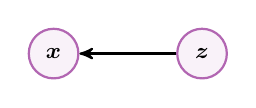
\begin{tikzpicture}[
        roundnode/.style={circle, draw=violet!60, fill=violet!5, minimum size=7mm},
        ->,>=stealth',auto,node distance=3.5em,thick]
        \tikzstyle{every node}=[font=\small,scale=0.9]
            \node[roundnode] (data) {$\bm{x}$};
            \node[roundnode, right = of data] (latent) {$\bm{z}$};
              
            \draw[->] (latent)  -- (data);
        \end{tikzpicture}
        }}
    \hskip5em
    \parbox{.35\textwidth}{%
        \subcaptionbox{M2\label{fig:vaem2}}{
        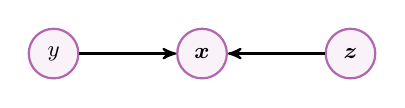
\begin{tikzpicture}[
        roundnode/.style={circle, draw=violet!60, fill=violet!5, minimum size=7mm},
        ->,>=stealth',auto,node distance=3.5em,thick]
        \tikzstyle{every node}=[font=\small,scale=0.9]
            \node[roundnode] (data) {$\bm{x}$};
            \node[roundnode, left = of data] (label) {$y$};
            \node[roundnode, right = of data] (latent) {$\bm{z}$};
              
            \draw[->] (latent) -- (data);
            \draw[->] (label) -- (data);
        \end{tikzpicture}
        }}
    \end{framed}
    }
    \caption{Two structures of VAE model in semi-supervised learning}
    \label{fig:vaem1m2}
\end{figure}


\textbf{Active learning} identify the true predictive mapping $y=f(\bm{x};\bm{\theta})$ by querying \textit{as few points as possible} such as in \textit{Bayesian optimization} and \textit{experiment design}.\unsure{
highlight choosing strategy of the labeled data points
}
\begin{itemize}
    \item \textbf{decision-theoretic approach}: explore a new point $\bm{x}$ with the minimal average \textit{risk increment} over all kind of output $y$ and parameters $\bm{\theta}$.
    \begin{align}
        U(\bm{x})\triangleq&~\mathbb{E}_{p(y|\bm{x}|\mathcal{D})}\left[
            \min_{a}(R(a|\mathcal{D})-R(a|\mathcal{D},(\bm{x},y)))
        \right]\\
        R(a|\mathcal{D}) =&~\mathbb{E}_{p(\bm{\theta}|\mathcal{D})}\ell(\bm{\theta},a)
    \end{align}

    \item \textbf{information-theoretic approach}: similar with the decision-theoretic one but considering to maximize \textit{information gain} about the parameters $\bm{\theta}$
    \begin{align}
        U(\bm{x}) =&~ \mathbb{H}(p(\bm{\theta}|\mathcal{D})) - \mathbb{E}_{p(y|\bm{x},\mathcal{D})}\mathbb{H}(p(\bm{\theta}|\mathcal{D},(\bm{x},y))) \\
        =&~ \mathbb{I}(\bm{\theta},y|\mathcal{D},\bm{x}) \\
        =&~ \underbrace{\mathbb{H}(p(y|\bm{x},\mathcal{D}))}_\text{\makecell{max. entropy\\ sampling}} - \underbrace{\mathbb{E}_{p(\bm{\theta}|\mathcal{D})}\mathbb{H}(p(y|\bm{x},\bm{\theta}))}_\text{\makecell{pick example with\\confident prediction}} \label{eq:actlearninfo}
    \end{align}
    which will select examples $\bm{x}$ making confident predictions which are highly diverse. 
    Therefore this approach is called \textbf{Bayesian active learning by disagreement (BALD)}.

    \item \textbf{batch active learning} or \textbf{BatchBALD}\unsure{
    The above strategies are greedy (myopic) search, select a optimal sample at one time.
    } collect a set of $B$ samples $(\mathbf{X}, \mathbf{Y})$ by a sequential greedy search, which is within a \textit{constant factor} of optimal.
\end{itemize}

 





% \begin{framed}{\large
% TODO list of the following week
% \begin{itemize}
%     % \item Finish read Chapter 19 Learning with Fewer Labeled Examples
%     \item Read Chapter 20 Dimensionality Reduction
% \end{itemize}
% }
% \end{framed}


% ############################### WK 13 #######################################


% \setcounter{section}{6}
% \setcounter{subsection}{1}
% \begin{center}
% \textit{Chapter 20 Dimensionality Reduction}
% \end{center}


% \subsection{Dimensionality Reduction}

\begin{table}[htpb]
    \centering
    \caption{Some short unfamiliar terminologies in Dimensionality Reduction}
    {\footnotesize

}
    {\small
    \begin{tabular}{cp{32em}}
        \toprule
        Terminology & Explanations \\
        \midrule
        \textbf{scree plot} & a plot of the eigenvalues $\lambda_l$ vs $l$ in order of decreasing magnitude \\
        \textbf{profile likelihood} & $L^*=\argmax\ell(L)$, assuming $\lambda_{1:L}\sim\mathcal{N}(\mu_1,\sigma^2)$ and $\lambda_{L+1:D}\sim\mathcal{N}(\mu_2,\sigma^2)$, $\ell(L)=\sum_{k=1}^L\log\mathcal{N}(\lambda_k|\hat{\mu}_1(L),\hat\sigma^2(L))+\sum_{k=L+1}^D\log\mathcal{N}(\hat\mu_2(L),\hat\sigma^2(L))$ \\
        \textbf{nonlinear factor analysis} & $p(\bm{x})=\int\mathcal{N}(\bm{x}|\bm{f}(\bm{z};\bm{\theta}),\mathbf{\Psi})\mathcal{N}(\bm{z}|\mathbf{0},\mathbf{I})d\bm{z}$ \\
        \textbf{\makecell{Exponential family\\factor analysis}} & $p(\bm{x}|\bm{z})=\exp\left\{\mathcal{T}(\bm{x})^\mathsf{T}\bm{\theta}+h(\bm{x})-g(\bm{\theta})\right\}$, whose posterior can not be calculated analytically due to the lack of conjugacy between exp-family likelihood and Gaussian prior \\
        \textbf{denoising autoencoder} & adding noise to its input, and the model reconstruct the clean version of original input, e.g. $p_c(\Tilde{\bm{x}}|\bm{x})=\mathcal{N}(\Tilde{\bm{x}}|\bm{x},\sigma^2\mathbf{I})$ and $\ell(\bm{x},r(\Tilde{\bm{x}}))=\|\bm{e}(\bm{x})\|^2_2$, where $\bm{e}(\bm{x})=r(\Tilde{\bm{x}}) - \bm{x}$ \\
        \textbf{contraction} & A linear operator with Jacobian $\mathbf{J}$ if $\|\mathbf{J}\bm{x}\|\leq 1$ for all unit-norm inputs $\bm{x}$. \\
        \textbf{Contractive autoencoder} & AE with additional penalty on \textit{encoder}'s Jacobian, $\Omega(\bm{z},\bm{x}) 
        = \lambda \left\|\frac{\partial \bm{f}_e(\bm{x})}{\partial \bm{x}}\right\|^2_F 
        = \lambda\sum_k \|\nabla_{\bm{x}}h_k(\bm{x})\|_2^2$.
        Cooperating with the reconstruction loss, this penalty forces the encoder to be a constant function encourages the model to learn a representation only a few units change in response to the variations of input. \\
        \textbf{sparse autoencoder} & AE with additional penalty on \textit{latent activations} $\Omega{\bm{z}}=\lambda\|\bm{z}\|_1$ (\textbf{activity regularization}) or for logistic units $\Omega(\bm{z}_{(1:L,1:N)})=\lambda\sum_k\infdiv{\bm{p}}{\bm{q}_k(\bm{z}_{(k,1:N)})}$ \\
        \textbf{manifold} & a topological space locally Euclidean.\\
        \textbf{manifold learning} & nonlinear dimensionality reduction, recovers the underlying low-dimensional structure in a high-dimensional dataset, where the low-dimensional structure is assumed to be a curved manifold (\textbf{manifold hypothesis}). \\
        \textbf{Isomap} & approximate the structure of manifold first by creating KNN graph 
        (using \texttt{Dijkstra}'s shortest path algorithm) between datapoints and 
        then apply classical MDS (i.e. PCA) on the new space to capture local structure. \\
        \bottomrule
    \end{tabular}}
    \label{tab:dimreduce}
\end{table}


\textbf{Principal components analysis (PCA)} finds a \textit{linear} and \textit{orthogonal} 
\textit{projection}\unsure{
    In the context of projection, 
    the \textbf{encoder} is defined as $\mathbf{W}^\mathsf{T}\bm{x}=\bm{z}$,
    and the \textbf{decoder} is defined as $\mathbf{W}\bm{z}=\hat{\bm{x}}$
} of the high dimensional data $\bm{x}$ to a low dimensional subspace $\bm{z}$, 
i.e. $\mathbf{W}^\mathsf{T}\in\mathbb{R}^{L\times D}:\mathbb{R}^D\to \mathbb{R}^L$, such that minimizes the \textbf{reconstruction error}
\begin{gather}
    \mathcal{L}(\mathbf{W})\triangleq\frac{1}{N}\sum_{n=1}^N\|\bm{x}_n-\underbrace{\text{Dec}(\text{Enc}(\bm{x}_n;\mathbf{W});\mathbf{W})}_{\hat{x}_n}\|_2^2 \\
    \Rightarrow\mathbf{U}_L=\mathbf{W}^*=\min_{\mathbf{W}}\mathcal{L}(\mathbf{W}),
\end{gather}
where $\mathbf{U}_L$ contains $L$ eigenvectors with the largest eigenvalues of the \textbf{empirical} covariance matrix,\unsure{
    By imposing a constraint of $\mathbf{W}^\mathsf{T}\mathbf{W}=\mathbf{I}$,
    we can solve this optimization problem by solving the KKT of its dual problem,
    $\hat{\mathbf{\Sigma}}\mathbf{W}=\mathrm{diag}(\lambda_1,\cdots,\lambda_L)\mathbf{W}$,
    where $\lambda_l$ is the $l$-th Lagrange multiplier introduced by Lagrange function,
    which has the same format of solving eigenvalue decomposition. 
    With the $L$ increasing, reconstruction loss of PCA will keep decreasing!
}\unsure{
    due to the orthogonal constraint, vectors $\bm{w}_l$ can be optimized one by one.
}
which is equivalent to maximizing the likelihood of \textit{a latent linear Gaussian model} known as probabilistic PCA.\unsure{
    PCA and the probabilistic PCA \textit{without} noise are the same thing.
}
One can show that
\begin{align}
    \mathcal{L}_L
    & = \sum_{l=L+1}^D \lambda_l \\
    \mathcal{F}_L
    & = \frac{\sum_{l=1}^L\lambda_l}{\sum_{l'=1}^D\lambda_{l'}},
\end{align}
where $\mathcal{F}_L$ is the \textbf{fraction of variance explained}.

Some computational issues appear in practice:
\begin{enumerate}[(1)]
    \item \uline{use correlation matrix to compute projection matrix}, which is equivalent to use the variance matrix of the data standardized to avoid the measurement scale effect.
    
    \item \uline{Eigenvalue-decompose the Gram matrix $\mathbf{XX}^\mathsf{T}$} 
    instead of covariance matrix $\mathbf{X}^\mathsf{T}\mathbf{X}$ to reduce the computational complexity 
    when $N<D$, and the eigenvectors of covariance matrix can be obtained by\unsure{
    Note computing PCA by Gram matrix we need to know the data matrix.
    }
    \begin{align}
        \mathbf{XX}^\mathsf{T}
        & = \Tilde{\mathbf{U}}\Tilde{\mathbf{\Lambda}}\Tilde{\mathbf{U}}^\mathsf{T} \label{eq:pcagram}\\
        \Rightarrow~~ 
        \underbrace{\mathbf{X}^\mathsf{T}\mathbf{X}}_\text{cov}\mathbf{X}^\mathsf{T}\Tilde{\mathbf{U}} 
        & = \underbrace{\mathbf{X}^\mathsf{T}\Tilde{\mathbf{U}}}_\text{\tiny\makecell{unnor-\\malized\\eigenvec}}\Tilde{\mathbf{\Lambda}} \\
        \Rightarrow~~
        \Aboxed{\mathbf{U} & =
        \mathbf{X}^\mathsf{T}\Tilde{\mathbf{U}}\Tilde{\mathbf{\Lambda}}^{-\frac{1}{2}}} \label{eq:pcagramsol} \\
        \text{since}~~
        \|\mathbf{X}^\mathsf{T}\Tilde{\bm{u}}_l\|_2^2
        & = \Tilde{\bm{u}}_l^\mathsf{T}\mathbf{XX}^\mathsf{T}\Tilde{\bm{u}}_l \\
        & = \Tilde{\lambda}_l
    \end{align}

    \item \uline{computing PCA using SVD of $\mathbf{X}$}\unsure{
        Recall Chapter 7, the truncated SVD approximation
    } and randomized SVD ($O(NL^2) + O(L^3)$) when very high-dimensional problems.
\end{enumerate}



\textbf{Factor analysis} corresponds to the following linear-Gaussian latent variable generative model:\unsure{
    The parameters to be determined are $\mathbf{W}$, $\bm{\mu}$, and $[\psi_1,\cdots,\psi_L]$
}
\begin{align}
    p(\bm{z}) 
    & = \mathcal{N}(\bm{z}|\mathbf{0},\mathbf{I}) \\
    p(\bm{x}|\bm{z})
    & = \mathcal{N}(\bm{x}|\mathbf{W}\bm{z}+\bm{\mu},\mathbf{\Psi}) ~~ \mathbf{\Psi}=\mathrm{diag}(\psi_1,\cdots,\psi_L) \\
    \Rightarrow p(\bm{x}) & = \mathcal{N}(\bm{x}|\bm{\mu},\underbrace{\mathbf{WW}^\mathsf{T}+\mathbf{\Psi}}_{\mathbf{C}}) ~~ \text{i.e.} \\
    \mathrm{Var}~x_d & = {\color{violet}\sum_{k=1}^L w_{dk}^2} + {\color{teal}\psi_d} \\
    & = \text{\color{violet}due to common factors} + \textbf{\color{teal}uniqueness}
\end{align}
Once it is fitted (by EM), then we can get the distribution of latent variables by Bayes rule 
\begin{gather}
    \boxed{p(\bm{z}|\bm{x}) = \mathcal{N}(\bm{z}|\hat{\mathbf{W}}^\mathsf{T}\hat{\mathbf{C}}^{-1}(\bm{x}-\hat{\bm{\mu}}),\mathbf{I}-\hat{\mathbf{W}}^\mathsf{T}\hat{\mathbf{C}}^{-1}\hat{\mathbf{W}})} \label{eq:faposterior}
\end{gather}

\textbf{Probabilistic PCA}: FA with additional constraints, that is\unsure{
    Then, the parameters to be determined remains $\mathbf{W}$ and $\sigma^2$.
}
\begin{gather}
    \begin{cases}
    \mathbf{W}~\text{has orthonormal columns} \\
    \psi_{1} = \cdots = \psi_{L} = \sigma^2 \\
    \bm{\mu} = \mathbf{0}
    \end{cases} \\
    \Rightarrow
    \mathrm{NLL} = - \log p(\mathbf{X}|\bm{\mu},\mathbf{W},\sigma^2) = \frac{N}{2}\left[
        D\log (2\pi) + \log |\mathbf{C}| + \mathrm{tr}(\mathbf{C}^{-1}\mathbf{S})
    \right],
\end{gather}
where $\mathbf{S} = \frac{1}{N} \sum_{n=1}^N(\bm{x}_n - \Bar{x})(\bm{x}_n - \Bar{x})^\mathsf{T}$,\unsure{
    This is the covariance matrix to be decomposed in PCA.
}
\begin{gather}
    \Rightarrow \begin{cases}
        \hat{\mathbf{W}}_\text{mle} = \mathbf{U}_L(\mathbf{L}_L - \sigma^2\mathbf{I})^\frac{1}{2}\mathbf{R}~~~(\forall~\mathbf{R}~\text{can be}~\mathbf{I}) \\
        \hat{\sigma}^2_\text{mle} = \frac{1}{D - L}\sum_{i=L+1}^D \lambda_i
    \end{cases}
\end{gather}
which can plugin FA's posterior inference (\ref{eq:faposterior})\unsure{
    The unidentifiability of FA results in the arbitrariness of $\mathbf{R}$, which is an orthogonal rotation matrix that transform the latent embedding to another. Since latent space is isotropic, any orthogonal rotation will not conflict the distribution assumption.
} and 
use matrix inverse lemma (Lemma \ref{eq:woodbury}) to avoid computing the inverse of $\mathbf{C}$\unsure{
    \color{red}On Page 665 of \cite{pml1Book}, the deduction of PPCA is incorrect.
}
\begin{align}
    \mathbf{C}^{-1} 
    & = \left[
        \sigma^2\mathbf{I} + \mathbf{WW}^\mathsf{T}
    \right]^{-1} \\
    & = \sigma^{-2}[\mathbf{I}-\mathbf{W}{\underbrace{(\sigma^2\mathbf{I} + \mathbf{W}^\mathsf{T}\mathbf{W})}_{\color{red}=\mathbf{L}_L}}^{-1}\mathbf{W}^\mathsf{T}] \\
    & = \sigma^{-2}\left[
        \mathbf{I} - \mathbf{U}_L(\mathbf{L}_L-\sigma^2\mathbf{I})\mathbf{L}_L^{-1}\mathbf{U}_L^\mathsf{T}
    \right] \\
    & = \sigma^{-2}\left[
        \mathbf{I} - \mathbf{U}_L(\mathbf{L}_L-\sigma^2\mathbf{I})^\frac{1}{2}\mathbf{L}_L^{-1}(\mathbf{L}_L - \sigma^2\mathbf{I})^\frac{1}{2}\mathbf{U}_L^\mathsf{T}
    \right]
\end{align}
\begin{gather}
    \Rightarrow ~\boxed{p(\bm{z}|\bm{x})
    = \mathcal{N}(\bm{z}|\mathbf{L}_L^{-1}\mathbf{W}^\mathsf{T}\bm{x}, \sigma^2\mathbf{L}_L^{-1})
    }
\end{gather}

\begin{example}[vanilla EM for FA]\label{example:em4fa}
$~$
    \begin{itemize}
        \item \textbf{E step}: for some given parameters $\bm{\theta}=[\mathbf{W},\bm{\mu},\mathbf{\Psi}]$,
        we can compute the posterior embeddings $\bm{z}_i$ for each observations $\bm{x}_i$
        \begin{align}
            p(\bm{z}_i|\bm{x}_i,\bm{\theta}) & = \mathcal{N}(\bm{z}_i|\bm{m}_i,\mathbf{\Sigma}_i) \\
            \bm{m}_i & \triangleq \mathbf{\Sigma}_i(\mathbf{W}^\mathsf{T}\mathbf{\Psi}^{-1}(\bm{x}_i-\bm{\mu})) \\
            \mathbf{\Sigma}_i & \triangleq (\mathbf{I} + \mathbf{W}^\mathsf{T}\mathbf{\Psi}^{-1}\mathbf{W})^{-1}
        \end{align}

        \item \textbf{M step}: compute the point estimation of $\bm{\theta}=[\Tilde{\mathbf{W}},\mathbf{\Psi}]$. 
        Define $\Tilde{\mathbf{W}}=[\mathbf{W},\bm{\mu}]$ and $\Tilde{\bm{z}}=[\bm{z},1]$
        \begin{align}
            \bm{b}_i & \triangleq \mathbb{E}[\Tilde{\bm{z}}|\bm{x}_i]=\begin{bmatrix}
                \bm{m}_i \\ 1
            \end{bmatrix} \\
            \mathbf{C}_i & \triangleq \mathbb{E}[\Tilde{\bm{z}}\Tilde{\bm{z}}^\mathsf{T}|\bm{x}_i] = \begin{bmatrix}
                \mathbb{E}[\bm{zz}^\mathsf{T}|\bm{x}_i] &\mathbb{E}[\bm{z}|\bm{x}_i] \\
                \mathbb{E}[\bm{z}|\bm{x}_i] & 1
            \end{bmatrix} \\
            \Rightarrow \hat{\Tilde{\mathbf{W}}} & = \left[
                \sum_{i=1}^N\bm{x}_i\bm{b}_i^\mathsf{T}
            \right]\left[
                \sum_{i=1}^N\mathbf{C}_i
            \right]^{-1} \\
            \hat{\mathbf{\Psi}} & = \frac{1}{N}\mathrm{diag}\left\{
            \sum_{i=1}^N(\bm{x}_i-\hat{\Tilde{\mathbf{W}}}\bm{b}_i)\bm{x}_i^\mathsf{T}
            \right\}
        \end{align}
    \end{itemize}
\end{example}


\begin{example}[EM for PPCA]
    Denote $\Tilde{\mathbf{X}} = \mathbf{X}^\mathsf{T}$
    \begin{itemize}
        \item \textbf{E step}: $\Tilde{\mathbf{Z}} = (\mathbf{W}^\mathsf{T}\mathbf{W})^{-1}\mathbf{W}^\mathsf{T}\Tilde{\mathbf{X}}$ 
        \item \textbf{M step}: $\Tilde{\mathbf{X}}\Tilde{\mathbf{Z}}^\mathsf{T}(\Tilde{\mathbf{Z}}\Tilde{\mathbf{Z}}^\mathsf{T})^{-1}$
    \end{itemize}
\end{example}




\textbf{Mixtures of factor analysers} assume the model is \textit{only locally linear} and 
the overall model is a combination of several FA models.\unsure{
    The formula in original text of \cite{pml1Book} is incorrect.
}
\begin{align}
    p(\bm{x}|\bm{z},c=k) 
    & = \mathcal{N}(\bm{x}|\mathbf{W}_k\bm{z}+\bm{\mu}_k,\mathbf{\Psi}_k) \\
    p(\bm{z}) 
    & = \mathcal{N}(\bm{z}|\mathbf{0},\mathbf{I}) \\
    p(c) 
    & = \mathrm{Cat}(c|\bm{\pi}) \\
    \Rightarrow~p(\bm{x}|\bm{\theta})
    & = \sum_k p(c=k)\int p(\bm{x}|\bm{z},c)p(\bm{z}|c)d\bm{z} \\
    & = \sum_k \pi_k\int \mathcal{N}(\bm{x}|\mathbf{W}_k\bm{z},\mathbf{\Psi}_k)\mathcal{N}(\bm{z}|\bm{\mu}_k,\mathbf{I}) d\bm{z}
\end{align}


Factor analysis models for paired data $(\bm{x},\bm{y})$\unsure{The methods below are not necessary under assumption of Gaussian but for examples}
\begin{itemize}
    \item \textbf{Supervised PCA} integrates the information of label to estimation 
    by modeling the joint $p(\bm{x},\bm{y})$ using a shared lower dimensional representation
    \begin{align}
        p(\bm(z)) 
        & = \mathcal{N}(\bm{z},\mathbf{0},\mathbf{I}) \\
        p(\bm{x}|\bm{z})
        & = \mathcal{N}(\bm{x}|\mathbf{W}_x\bm{z},\sigma_x^2\mathbf{I}) \\
        p(\bm{y}|\bm{z})
        & = \mathcal{N}(\bm{y}|\mathbf{W}_y\bm{z},\sigma_y^2\mathbf{I}) \\
        \overset{y\in\mathbb{R}}{\Rightarrow} 
        p(y|\bm{x},\bm{\theta}) 
        & = \mathcal{N}(y|\bm{x}^\mathsf{T}\bm{v},\bm{w}_y^\mathsf{T}\mathbf{C}\bm{w}_y+\sigma_y^2) \\
        \mathbf{C}
        & \triangleq (\mathbf{I}+\sigma_x^{-2}\mathbf{W}_x^\mathsf{T}\mathbf{W}_x)^{-1} \\
        \bm{v}
        & \triangleq \sigma_x^{-2}\mathbf{W}_x\mathbf{C}\bm{w}_y.
    \end{align}
    This model is completely symetric in $\bm{x}$ and $\bm{y}$, and the part to be predicted in the likelihood can be upweighted by
    \begin{gather}
        p(\mathbf{X}, \mathbf{Y}, \mathbf{Z}|\bm{\theta}) = p(\mathbf{Y}|\mathbf{Z},\mathbf{W}_y)p(\mathbf{X}|\mathbf{Z},\mathbf{W}_x)^\alpha p(\mathbf{Z})~~~\alpha \leq 1
    \end{gather}
    
    \item \textbf{Partial least squares} allow the inputs $\bm{x}$ to have their own \textit{additional} ``private'' noise source $(\bm{z}_x,\bm{b}_x)$ that is independent on the target variable $\bm{y}$
    \begin{align}
        p(\bm{z}) 
        & = \mathcal{N}(\bm{z}_s|,\mathbf{0},\mathbf{I})\mathcal{N}(\bm{z}_x|\mathbf{0},\mathbf{I}) \\
        p(\bm{x}|\bm{z})
        & = \mathcal{N}(\bm{x}|\mathbf{W}_x\bm{z}_s+\mathbf{B}_x\bm{z}_x,\sigma_x^2\mathbf{I}) \\
        p(\bm{y}|\bm{z})
        & = \mathcal{N}(\bm{y}|\mathbf{W}_y\bm{z}_s,\sigma_y^2\mathbf{I})
    \end{align}

    \item \textbf{Canonical correlation analysis}, similar with the partial least squares, also introduce \textit{additional} ``private'' noise sources for \textit{both} $\bm{x}$ and $\bm{y}$\unsure{
        When the dimension of latent space is set to 1, then the \textbf{CCA} model can be applied to measure the correlation of two \textit{arbitrary-dimension} variables, 
        which has been widely used in analysis the connectome of high-dimensional brain images.
    }
    \begin{align}
        p(\bm{z})
        & = \mathcal{N}(\bm{z}_s|\mathbf{0},\mathbf{I})\mathcal{N}(\bm{z}_x|\mathbf{0},\mathbf{I}) \\
        p(\bm{x}|\bm{z})
        & = \mathcal{N}(\bm{x}|\mathbf{W}_x\bm{z}_s+\mathbf{B}_x\bm{z}_x,\sigma_x^2\mathbf{I}) \\
        p(\bm{y}|\bm{z})
        & = \mathcal{N}(\bm{y}|\mathbf{W}_y\bm{z}_s+\mathbf{B}_y\bm{z}_y,\sigma_y^2\mathbf{I}) \\
        \Rightarrow p(\bm{x},\bm{y}) 
        & = \mathcal{N}(\bm{x},\bm{y}|\bm{\mu},\mathbf{WW}^\mathsf{T} + \sigma^2\mathbf{I}) \\
        \bm{\mu}
        & = [\bm{\mu}_x;\bm{\mu}_y] \\
        \mathbf{W}
        & = \left[\mathbf{W}_x;\mathbf{W}_y\right] \\
        \mathbf{WW}^\mathsf{T}
        & = \begin{bmatrix}
            \mathbf{W}_x\mathbf{W}_x^\mathsf{T} & \mathbf{W}_x\mathbf{W}_y^\mathsf{T} \\
            \mathbf{W}_y\mathbf{W}_x^\mathsf{T} & \mathbf{W}_y\mathbf{W}_y^\mathsf{T}
        \end{bmatrix}
    \end{align}
\end{itemize}



\textbf{Variational autoencoder} has two components and EM-like loss: 
\begin{enumerate}[(1)]
    \item the decoder is a non-linear extension of the \textit{factor analysis generative model}
    \begin{gather}
        p_{\bm{\theta}}(\bm{x}|\bm{z}) = \begin{cases}
            \mathcal{N}(\bm{x}|\bm{f}_d(\bm{z};\bm{\theta}),\sigma^2\mathbf{I}) & \text{continuous} \\
            \prod_{i=1}^D\mathrm{Ber}(x_i|f_d(\bm{z};\bm{\theta})) & \text{binary}
        \end{cases}
    \end{gather}

    \item the encoder, \textbf{inference network}, is trained simultaneously with generative model to do \textit{approximate posterior} inference
    \begin{gather}
        q_{\phi}(\bm{z}|\bm{x}) = \mathcal{N}(\bm{z}|\underbrace{\bm{f}_{e_\mu}(\bm{x};\bm{\phi}_\mu)}_{\bm{\mu}_{\bm{\phi}}(\bm{x})},\mathrm{diag}(\underbrace{\bm{f}_{e_\sigma}(\bm{x};\bm{\phi}_\sigma)}_{\bm{\sigma}_{\bm{\phi}}(\bm{x})})) ~~~ \text{e.g. continuous}.
    \end{gather}

    \item loss function
    \begin{align}
        \log p_{\bm{\theta}}(\bm{x}) 
        & = {\color{blue}\log} \int q_{\bm{\phi}}(\bm{z}|\bm{x})\frac{p_{\bm{\theta}}(\bm{x},\bm{z})}{q_{\bm{\phi}}(\bm{z}|\bm{x})} d\bm{z} \\
        & \geq  \int q_{\bm{\phi}}(\bm{z}|\bm{x}) {\color{blue}\log} \frac{p_{\bm{\theta}}(\bm{x},\bm{z})}{q_{\bm{\phi}}(\bm{z}|\bm{x})} d\bm{z} \\
        & = \mathbb{E}_{q_{\bm{\phi}}(\bm{z}|\bm{x})} {\color{blue}\log} \frac{p_{\bm{\theta}}(\bm{x}|\bm{z})p(\bm{z})}{q_{\bm{\phi}}(\bm{z}|\bm{x})} \\
        & = \underbrace{\mathbb{E}_{q_{\bm{\phi}}(\bm{z}|\bm{x})} {\color{blue}\log} p_{\bm{\theta}}(\bm{x}|\bm{z}) - \overbrace{\mathbb{E}_{q_{\bm{\phi}}(\bm{z}|\bm{x})} {\color{blue}\log} \frac{q_{\bm{\phi}}(\bm{z}|\bm{x})}{p(\bm{z})}}^{\infdiv{q_{\bm{\phi}}(\bm{z}|\bm{x})}{p(\bm{z})}}}_{\L(\bm{\theta},\bm{\phi}|\bm{x})} \\
        & = \mathbb{E}_{\bm{\epsilon}\sim\mathcal{N}(\mathbf{0},\mathbf{I})} {\color{blue}\log} p_{\bm{\theta}}(\bm{x}|\bm{z}=\bm{\mu}_{\bm{\phi}}(\bm{x}) + \bm{\sigma}_{\bm{\phi}}(\bm{x}) \odot \bm{\epsilon}) - \infdiv{q_{\bm{\phi}}(\bm{z}|\bm{x})}{p(\bm{z})}
    \end{align}
\end{enumerate}


\textbf{Multidimensional scaling (MDS)} tries to find a set of low dimensional vectors $\bm{z}_i\in\mathbb{R}^L,i=1,\cdots,N$ 
such that their \textit{pairwise distances} are as similar as possible to pairwise dissimilarities of the original data provided by user.
\begin{enumerate}[(1)]
    \item \uline{classic MDS} defines the dissimilarity by the kernel of centered original data $\Tilde{\mathbf{K}}=\Tilde{\mathbf{X}}\Tilde{\mathbf{X}}^\mathsf{T}$, 
    \textit{equivalent to PCA}.
    \begin{gather}
        \mathcal{L}_\text{\color{violet}strain}(\mathbf{Z}) = \sum_{i,j}\left(
            \Tilde{K}_{ij} - \langle\Tilde{\bm{z}}_i,\Tilde{\bm{z}}_j\rangle
        \right)^2
        = \left\|\Tilde{\mathbf{K}}-\Tilde{\mathbf{Z}}\Tilde{\mathbf{Z}}^\mathsf{T}\right\|^2_F
    \end{gather}

    \item \uline{metric MDS} generalizes to allow for \textit{any} dissimilarity measure. 
    \begin{gather}
        \mathcal{L}_\text{\color{violet}stress}(\mathbf{Z}) = \sqrt{\frac{\sum_{i<j}\left(d_{ij}-\hat{d}_{ij}\right)^2}{\sum_{i,j}d_{ij}^2}}, 
    \end{gather}
    where $\hat{d}_{ij}=\|\bm{z}_i-\bm{z}_j\|$.

    \item \uline{non-metric MDS} matches the ranking  of how similar points are instead of similarity measure.
    \begin{gather}
        \mathcal{L}_\text{\color{violet}NM}(\mathbf{Z}) = \sqrt{\frac{\sum_{i<j}\left(f(d_{ij})-\hat{d}_{ij}\right)^2}{\sum_{i,j}\hat{d}_{ij}^2}},
    \end{gather}
    where $\hat{d}_{ij}=\|\bm{z}_i-\bm{z}_j\|$ and $f(d)$ is a monotonic transformation from distances to ranks.

    \item \uline{Sammon mapping} upweights small distances since it matter more in many embedding methods comparing with metric MDS.
    \begin{gather}
        \mathcal{L}_\text{\color{violet}sammon}(\mathbf{Z})=\frac{1}{\sum_{i<j}d_{ij}}\sum_{i\neq j}\frac{(d_{ij}-\hat{d}_{ij})^2}{d_{ij}}
    \end{gather}
\end{enumerate}


\textbf{Kernel PCA} replaces the Gram matrix $\mathbf{XX}^\mathsf{T}$ in Equation (\ref{eq:pcagram}) to a kernel $\mathcal{K}(\mathbf{X},\mathbf{X})$.
If we denote the kernel function's implicit feature representation as $\mathcal{K}(\bm{x}_i,\bm{x}_j)=\bm{\phi}(\bm{x}_i)^\mathsf{T}\bm{\phi}(\bm{x}_j)$,\unsure{
    But the feature representation is unknown or infinite dimensiona,
    we can only get the projection of new data directly.
}
then by Equation (\ref{eq:pcagramsol}), the projection matrix is 
\begin{gather}
    \mathbf{U}_\text{kpca} = \mathbf{\Phi}^\mathsf{T}\Tilde{\mathbf{U}}\Tilde{\Lambda}^{-\frac{1}{2}} \\
    \Rightarrow \bm{\phi}_*^\mathsf{T}\mathbf{U}_\text{kpca} = \bm{k}_*^\mathsf{T}\Tilde{\mathbf{U}}\Tilde{\mathbf{\Lambda}}^{-\frac{1}{2}},
\end{gather}
where $\bm{k}_*^\mathsf{T} = [\mathcal{K}(\bm{x}_*,\bm{x}_1),\cdots,\mathcal{K}(\bm{x}_*,\bm{x}_N)]$ and 
$\bm{x}_*$ is a new test datapoint whose feature representation is $\bm{\phi}_*$.
However, kernel PCA does not reduce the dimension of feature but expand it if using rbf kernel function for example.
This problem can be solved by stacking \textbf{maximum variance unfolding} (MVU) to learn a kernel defined on a lower dimensional embedding $\bm{\phi}_i=\bm{z}_i$
\begin{align}
    \max~\sum_{(i,j)\in\mathcal{G}}\|\bm{z}_i-\bm{z}_j\|^2_2~~\text{s.t.}&~~\|\bm{z}_i-\bm{z}_j\|_2^2 = \|\bm{x}_i-\bm{x}_j\|_2^2 \\
    \iff& \\
    \max~\mathrm{tr}(\mathbf{K}(=\mathbf{ZZ}^\mathsf{T}))~~\text{s.t.}&~~\begin{cases}
        \|\bm{z}_i-\bm{z}_j\|_2^2 = \|\bm{x}_i-\bm{x}_j\|_2^2 \\
        \sum_{i,j} K_{ij} = 0 \\
        \mathbf{K} \succ 0
    \end{cases},
\end{align}
where $\mathcal{G}$ is the nearest neighbor graph such as from Isomap.\unsure{
    It is like metric MDS but in a unfolded data manifold or Isomap with metric MDS.
}


\textbf{LLE}, local linear embedding, assumes the data manifold around each point $\bm{x}_i$ is locally linear and find linear approximation (reconstruction weights $\bm{w}_i$) by predicting $\bm{x}_i$ as linear combination of its $K$ nearest neighbors both in original space and transfer the approximation to embedding space to reduce the dimension. \unsure{
    Compared with Isomap, LLE is less sentive to \textit{short-circuiting} (noise).
}
\begin{align}
    \hat{\mathbf{W}} & = \argmin_{\mathbf{W}}\sum_{i=1}^N\left(
        \bm{x}_i - \sum_{i=1}^N w_{ij}\bm{x}_j
    \right)^2~~\text{s.t.}~~ \begin{cases}
        w_{ij} = 0 & \bm{x}_{ij}\notin\mathcal{N}_K(\bm{x}_i) \\
        \sum_{j=1}^N w_{ij} = 1 & i=1,\cdots,N
    \end{cases} \\
    \hat{\mathbf{Z}} & = \argmin_{\mathbf{Z}}\|\mathbf{Z}-\hat{\mathbf{W}}\mathbf{Z}\|^2_2
\end{align}



\textbf{Laplacian eigenmaps}, or \textbf{spectral embedding}, computes a low-dimensional representation of the data 
where the \textit{weighted distances} between a datapoint and its $K$ \textit{nearest neighbors} are minimized
and the weights decay with the distances increasing.
\begin{align}
    \mathcal{L}(\mathbf{Z}) & = \sum_{i,j}W_{ij}\|\bm{z}_i-\bm{z}_j\|^2_2~~\mathrm{s.t.}~~\mathbf{Z}^\mathsf{T}\mathbf{DZ}=\mathbf{I} \\
    W_{ij} & \triangleq \begin{cases}
        \exp\left(-\frac{1}{2\sigma^2}\|\bm{x}_i-\bm{x}_j\|\right) & j\in\mathcal{N}_K(i) \\
        0 & \text{otherwise}
    \end{cases} \\
    \mathbf{D} & \triangleq \mathrm{diag}(D_{ii}=\sum_{j}W_{ij}) ~~~\text{(degree of each node)} \\
    \Rightarrow
    \mathcal{L}(\mathbf{Z}) & = 2\mathrm{tr}(\mathbf{Z}^\mathsf{T}(\underbrace{\mathbf{D}-\mathbf{W}}_{\mathbf{L}})\mathbf{Z}) \\
    \min_{\mathbf{Z}} \mathcal{L}(\mathbf{Z}) & \iff \mathbf{L}\bm{z}_i = \lambda_i\mathbf{D}\bm{z}_i,i=1,\cdots,L ~\text{smallest nonzero eigenvalues}
\end{align}
where the $\mathbf{L}$ is the \textbf{graph Laplacian}\unsure{
    recall the fundamental GCN, Laplacian matrix $\mathbf{L}\triangleq\mathbf{D}-{\color{blue}\mathbf{A}}$ implies the connectome of graph and the smoothness path of information.
}
It can serve as a differentiation operator to compute a discrete derivative of the function at a point $i$\unsure{
    \textit{gradient} at node $i$
} or an overall measure of ``smoothness'' of the function $f$\unsure{
    \textit{Hessian} of $f$ over the graph.
}:
\begin{align}
    [\mathbf{L}\bm{f}]_i 
    & = \sum_{j\in\mathcal{N}(i)}W_{ij}[\bm{f}_i-\bm{f}_j] \\
    \bm{f}^\mathsf{T}\mathbf{L}\bm{f} 
    & = \bm{f}^\mathsf{T}\mathbf{D}\bm{f} - \bm{f}^\mathsf{T}\mathbf{W}\bm{f} 
    = \sum_{i}d_if_i^2 - \sum_{i,j}w_{ij}f_if_j \\
    & = \frac{1}{2}\left(\sum_i d_if_i^2 - 2\sum_{i,j}w_{ij}f_if_j + \sum_j d_jf_j^2\right) \\
    & = \frac{1}{2}\sum_{i,j}w_{ij}(f_i-f_j)^2~~~(\geq 0~\forall\bm{f}\Rightarrow \mathbf{L}\succeq 0)
\end{align}











% \begin{framed}{\large
% TODO list of the following week
% \begin{itemize}
%     \item Finish Chapter 20 Dimensionality Reduction (10 pages remaining: t-SNE and word embeddings);
%     \item Read \cite{cang_screening_2023} and prepare for group meeting;
%     \item Try to finish Chapter 21 Clustering;
% \end{itemize}
% }
% \end{framed}


% ############################### WK 14 #######################################


% \setcounter{section}{6}
% \setcounter{subsection}{2}
% \begin{center}
% \textit{Rest of Chapter 20 Dimensionality Reduction \& Chapter 21 Clustering}
% \end{center}

% \begin{table}[htpb]
    \centering
    \caption{Some short unfamiliar terminologies in Remaining chapter}
    {\footnotesize

}
    {\small
    \begin{tabular}{cp{32em}}
        \toprule
        Terminology & Explanations \\
        \midrule
        \textbf{UMAP} & Uniform Manifold Approximation and Projection, similar to tSNE at a high level 
        but tends to \textit{preserve global structure} better and is much faster. \\
        \textbf{\makecell[t]{term-document\\frequency matrix}} & $\mathbf{C}\in\mathbb{R}^{M\times N}$, $C_{ij}$ be the number of times \textit{term} $i$ occurs in \textit{context} $j$, which is a simplified TF-IDF. \\
        \textbf{\makecell[t]{latent semantic\\indexing}} & $\mathbf{C}\approx\hat{\mathbf{C}}=\mathbf{USV}^\mathsf{T}$, $\mathbf{U}\in\mathbb{R}^{M\times L}$ are the embeddings for $M$ \textit{words}, and 
        $\mathbf{VS}=[\bm{v}_j\odot\bm{s}]_{j=1:N}\in\mathbb{R}^{N\times L}$ are the embeddings for $N$ \textit{documents}. \\
        \textbf{\makecell[t]{latent semantic\\analysis}} & same with LSI but with a finer grained $\mathbf{C}$ defined on the \textit{context of window $h$}, representing the \textbf{co-occurring} probability of maximum $h$ words. \\
        \textbf{\makecell[t]{pointwise mutual\\information}} & $C_{ij}=\mathrm{PMI}(i,j)\triangleq\log\frac{p(i,j)}{p(i)p(j)}$ or $[\mathrm{PMI}(i,j)]_+$, another substitution of term-document frequency matrix for the latent semantic preprocessing above \\
        \textbf{GLOVE} & global vectors for word representation \\
        \textbf{Word analogies} & ``man is to woman as king is to queen.'' \\
        \textbf{Rand-walk model} & $p(w_t=w|\bm{z}_t)=\exp(\bm{z}_t^\mathsf{T}\bm{v}_w)/\underbrace{\sum_{w'}\exp(\bm{z}_t^\mathsf{T}\bm{v}_{w'})}_{Z(\bm{z}_t)}$, assuming the prior for the word embeddings $\bm{v}_t$ is an isotropic Gaussian and the latent topic $\bm{z}_t$ undergoes a slow Gaussian random work, which can interpret the word embedding methods. \\
        \bottomrule
    \end{tabular}}
    \label{tab:rest}
\end{table}



\textbf{Stochastic neighborhood embedding (SNE)} converts high-dimensional Euclidean distances, 
including original data space and embedding space, into conditional probabilities that represent similarities.
\unsure{
    This idea is similar with MDS but uses conditional probability of picking datapoint $j$ given datapoint $i$
    as the similarity measure.
}
\begin{gather}
    \begin{cases}
        p_{j|i} = \frac{\exp\left(-\frac{1}{2\sigma_i^2}\|\bm{x}_i-\bm{x}_j\|^2_2\right)}{\sum_{k\neq i}\exp\left(-\frac{1}{2\sigma_i^2}\|\bm{x}_i-\bm{x}_k\|^2_2\right)} \\
        q_{j|i} = \frac{\exp\left(-\|\bm{z}_i-\bm{z}_j\|^2_2\right)}{\sum_{k\neq i}\exp\left(-\|\bm{z}_i-\bm{z}_k\|^2_2\right)}
    \end{cases}\\
    \mathcal{L}(\mathbf{Z}) = \sum_{i}\infdiv{P_i}{Q_i} = \sum_i\sum_j p_{j|i}\log\frac{p_{j|i}}{q_{j|i}} \\
    \nabla_{\bm{z}_i}\mathcal{L}(\mathbf{Z}) = 2\sum_{j}(\bm{z}_j-\bm{z}_i)(p_{j|i}-q_{j|i}+p_{i|j}-q_{i|j})
\end{gather}
Intuitively, $q_{j|i}$ should match $p_{j|i}$ if the embedding is good. 
The points are pulled towards each other if the $p$'s are bigger than the $q$'s, 
and repelled if the $q$'s are bigger than the $p$'s.
However, the objective is not convex and needs SGD for optimization.
\begin{itemize}
    \item \textbf{Symmetric SNE} simplifies the conditional probability to a symmetric one and has similar result with classic SNE.
    \begin{gather}
        \begin{cases}
            p_{ij} = \frac{\exp\left(-\frac{1}{2\sigma^2}\|\bm{x}_i-\bm{x}_j\|^2_2\right)}{\sum_{k<l}\exp\left(-\frac{1}{2\sigma^2}\|\bm{x}_k-\bm{x}_l\|^2_2\right)} \\
            q_{ij} = \frac{\exp\left(-\|\bm{z}_i-\bm{z}_j\|^2_2\right)}{\sum_{k<l}\exp\left(-\|\bm{z}_k-\bm{z}_l\|^2_2\right)}
        \end{cases}\\
        \mathcal{L}(\mathbf{Z}) = \sum_{i}\infdiv{P}{Q} = \sum_{i<j} p_{ij}\log\frac{p_{ij}}{q_{ij}} \\
        \nabla_{\bm{z}_i}\mathcal{L}(\mathbf{Z}) = 2\sum_{j}(\bm{z}_j-\bm{z}_i)(p_{ij}-q_{ij})
    \end{gather}

    \item \textbf{t-distributed SNE}, comparing with \textit{symmetric SNE}, 
    uses heavy tail distribution ($\nu=1$ Student-t, i.e. Cauchy) to calculate probability in embedding space
    to solve the \textit{crowding problem} brought by Gaussian distribution, 
    which tends to squeeze points that are relatively far away in the high dimensional space close together in the low dimensional embedding space\unsure{
        \color{red}Why this problem can arise due to non-heavy tail distribution?
    }
    \begin{gather}
        q_{ij}=\frac{\left(1+\|\bm{z}_i-\bm{z}_j\|_2^2\right)^{-1}}{\sum_{k<l}\left(1+\|\bm{z}_k-\bm{z}_l\|_2^2\right)^{-1}} \\
        \nabla_{\bm{z}_i}\mathcal{L}(\mathbf{Z}) = 4\sum_{j}(p_{ij}-q_{ij})\underbrace{(\bm{z}_i-\bm{z}_j){\color{blue}(1+\|\bm{z}_i-\bm{z}_j\|^2)^{-1}}}_{\bm{w}}
    \end{gather}
    where $(1+\|\bm{z}_i-\bm{z}_j\|^2)^{-1}$ lets points in embedding space act like stars and galaxies, 
    forming many \textbf{well-separated} clusters (galaxies) each of which has many stars tightly packed inside.\unsure{
        From the gradient, we can see the distribution difference of $p_{ij}$ and $q_{ij}$ only takes an effect within a local range and slowly decays with the distance increasing,
        which means only close points affect learning of congregation, but the distance between remote points will not or take few effect. 
        The bandwidth $\sigma^2$ controls the distance of neighbors such that is close enough to affect the learning.
    }
\end{itemize}

\begin{figure}[htpb]
    \centering
    \includestandalone[width=.8\textwidth]{figs/cauchypdf_raw}
    \caption{Plots of $x(1-x^2)^{-1}$ and $(1-x^2)^{-1}$}
    \label{fig:cauchypdf}
\end{figure}

\textbf{Word2vec} are \textit{shallow} neural nets for predicting a word given its context.
\begin{itemize}
    \item \textbf{CBOW}: continuous bag of words. For a seq of words $\bm{w}$ of length $T$, its log-likelihood is defined as follow, i.e., \uline{each word is predicted from its context}.\unsure{
        Every word depends on its neighbors within the distance of radius $m$.
    }\unsure{
        The formula here seems incorrect.
    }
    \begin{align}
        \log p(\bm{w}) & = \sum_{t=1}^T\log p(w_t|\bm{w}_{(t-m):(t+m)})=\sum_{t=1}^T\log\frac{\exp(\bm{v}_{w_t}^\mathsf{T}\bar{\bm{v}}_{\color{red}t})}{\sum_{t'}\exp(\bm{v}_{w_{t'}}^\mathsf{T}\Bar{\bm{v}}_{\color{red}t})} \\
        \bar{\bm{v}}_{\color{red}t} & \triangleq \frac{1}{2m}\sum_{h=1}^m(\bm{v}_{w_{t-h}}+\bm{v}_{w_{t+h}})
    \end{align}

    \item \textbf{Skip-gram} \uline{predict the context given each word}
    \begin{align}
        \log p(\bm{w}) & = \sum_{t=1}^T\sum_{-m\leq j\leq m}\log p(w_{t+j}|w_t) \\
        \log p(w_o|w_c) & = \bm{v}_{w_o}^\mathsf{T}\bm{v}_{w_c} - \log\sum_{i\in\mathcal{V}}\exp(\bm{v}_{w_i}^\mathsf{T}\bm{v}_{w_c})
    \end{align}
    Since the vanilla skip-gram should compute the preactivations for the entire vocabulary, computationally intensive,
    a set of $K+1$ \textit{context words} is sampled for each central word, $w_t$, to substitute the vocabulary related term, 
    called \textbf{Negative sampling}.
    In the sampled \textit{context words}, only one term is indeed in context of central words, $w_{t+j}$, $j=-m,\cdots,m$,
    and the remaining $K$ words, $\mathcal{K}$, are sampled from vocabulary according to a reweighed unigram distribution, 
    $w_k\sim p(w)\propto\mathrm{freq}(w)^\frac{3}{4}$\unsure{
        common words have larger probabilities to be sampled, while rare words have smaller ones.
    }
    \begin{align}
        p(w_{t+j}|w_t) & \approx p(D=1|w_t,w_{t+j})\prod_{k\in\mathcal{K}} p(D=0|w_t,w_k) \\
        p(D=1|w_t,w_{t+j}) & = \sigma(\bm{v}_{w_{t+j}}^\mathsf{T}\bm{v}_{w_t}) \\
        p(D=0|w_t,w_k) & = 1 - \sigma(\bm{v}_{w_k}^\mathsf{T}\bm{v}_{w_t})
    \end{align}
\end{itemize}



% \begin{framed}{\large
% TODO list of the following week
% \begin{itemize}
%     \item Read Chapter 22 Recommender Systems, \& Chapter 23 Graph Embeddings;
% \end{itemize}
% }
% \end{framed}


% ############################### WK 15 (Summer makeup) #######################################

\setcounter{section}{6}
\setcounter{subsection}{2}
\begin{center}
\textit{Rest of the book: Chapter 21 Clustering, 
Chapter 22 Recommender Systems, \& Chapter 23 Graph Embeddings}
\end{center}

\begin{table}[htpb]
    \centering
    \caption{Some short unfamiliar terminologies in Remaining chapter}
        \textit{The noting of Section 2-4 are skipped.}
    {\small
    \begin{tabular}{cp{32em}}
        \toprule
        Terminology & Explanations \\
        \midrule
        \textbf{BIC} & $\text{BIC}(K) = \log p(\mathcal{D}|\hat{\bm{\theta}}_k) - \frac{D_K}{2}\log N$, $D_K$ is the number of parameters in a model with $K$ clusters \\
        \textbf{label switching problem} & permuting the labels in a mixture model without changing the likelihood. \\
        \textbf{ordering constraint} & $\ell'(\bm{\theta}) = \log p(\mathcal{D}|\bm{\theta})+\log p(\bm{\theta})+\phi(\bm{\mu})$, 
        where $\phi(\bm{\mu})=-\infty$ if $\mu_1<\mu_0$ else $0$, where $\bm{\mu}$ is the label. \\
        \textbf{Collaborative filtering} & $\hat{Y}_{u,i}=\sum_{u':Y_{u',i}\neq ?}\mathrm{Sim}(u,u')Y_{u',i}$, 
        users collaborate on recommending items by sharing their ratings with other users \\
        \textbf{Matrix factorization} & $\mathcal{L}(\mathbf{Z}) = \|\mathbf{UV}^\mathsf{T}-\mathbf{Y}\|_\mathsf{F}^2$, $\mathbf{U}\in\mathbb{R}^{M\times K}$ and $\mathbf{V}\in\mathbb{R}^{N\times K}$, optimized by \textbf{ALS} or SGD when with missingness, and user-/item-specific baselines and penalty constraints can be added. \\
        \textbf{ALS} & Alternative least squares, estimating $\mathbf{U}$ given $V$ and vice versa \\
        \textbf{PMF} & Probabilistic matrix factorization, $p(y_{ui}=y)=\mathcal{N}(y|\mu+b_u+c_i+\bm{u}_u^\mathsf{T}\bm{v}_i,\sigma^2)$, allowing discrete distribution and regarding r/c symmetrically. \\
        \textbf{AutoRec} & $f(\bm{y}_{\cdot,i};\bm{\theta})=\mathbf{W}^\mathsf{T}\varphi(\mathbf{V}\bm{y}_{\cdot,i}+\bm{\mu})+\bm{b}$,
        \textit{item-based} nonlinear version of MF, there is also \textit{user-based}.\\
        \textbf{BPR} loss & Bayesian personalized ranking loss, $\mathcal{L}(\bm{\theta})=\sum_{(u,i,j)\in\mathcal{D}}\log \sigma(f(u,i;\bm{\theta})-f(u,j;\bm{\theta}))-\lambda\underbrace{\|\bm{\theta}\|^2}_{\mathcal{N}~\text{prior}}$, where $\mathcal{D}=\left\{(u,i,j):i\in\mathcal{I}_u^+,j\in\mathcal{I}\setminus\mathcal{I}_u^+\right\}$
        \textit{still asymmetrically}\\
        % \textbf{FM} & Factorization machines,  \\
        \textbf{GDL} & Geometric Deep Learning, applying deep learning techniques to non-Euclidean data \\
        \textbf{GRL} & Graph Representation Learning, learning low-dimensional continuous vector representations for graph-structured data, also called embedding \\
        \textbf{transductive} & the graph structure can be fixed throughout training and testing \\
        \textbf{inductive} & expecting to inference the info of graphs not seen during training \\
        \textbf{shallow graph embeddings} & $\mathbf{Z}=\mathrm{ENC}(\mathbf{\Theta}^E)\triangleq \mathbf{\Theta}^E$ where $\mathbf{\Theta}^E\in\mathbb{R}^{N\times L}$, the embedding dictionary $\mathbf{Z}$ is directly learned as model parameters, \textit{recall PCA} \\
        % \textbf{DeepWalk} & $\mathcal{L}_{G,\text{rec}}(\mathbf{W},\hat{\mathbf{W}};\mathbf{\Theta})=\log$ \\
        \textbf{Label propagation} & $\mathcal{L}_{G,\text{rec}}(\mathbf{W},\hat{\mathbf{W}};\mathbf{\Theta})=\sum_{i,j}W_{i,j}\|\bm{y}_i^N-\hat{y}_j^N\|^2_2$ \\
        \textbf{Label spreading} & $\mathcal{L}_{G,\text{rec}}(\mathbf{W},\hat{\mathbf{W}};\mathbf{\Theta})=\sum_{i,j}W_{i,j}\left\|\frac{\bm{y}_i^N}{\sqrt{D_i}}-\frac{\hat{y}_j^N}{\sqrt{D_j}}\right\|^2_2$ \\
        \bottomrule
    \end{tabular}}
    \label{tab:rest}
\end{table}




\subsection{Clustering}

Evaluating the clustering: to assign points that are similar to the same cluster, 
and to ensure that points that are dissimilar are in different clusters:
\begin{itemize}
    \item \textbf{Purity}: let $N_{ij}$ be the number of objects in cluster $i$ that belong to class $j$
    \begin{gather}
        \text{purity} \triangleq \sum_i
        \underbrace{\frac{\cancel{N_{i\cdot}}}{N_{\cdot\cdot}}}_\text{\makecell{cluster\\weight}}
        \underbrace{\max_j\frac{N_{ij}}{\cancel{N_{i\cdot}}}}_\text{\makecell{cluster\\purity}}
    \end{gather}

    \item \textbf{Rand index}: let $U=\{u_1,\cdots,u_R\}$ (estimated clustering) and 
    $V=\{v_1,\cdots,v_C\}$ (reference clustering) be two different \textit{partitions} of $N$ data points,
    and consider pairs of data points $(x_i,x_j)$\unsure{Hint: there are $\binom{N}{2}$ pairs.}
    having following relationship annotated by the two clustering labels:
    \begin{center}
        \begin{tabular}{ccc}
            \toprule
            estimated labels & reference labels & Notation \\
            \midrule
            $y^U_i = y^U_j$ & $y^V_i=y^V_j$ & $\mathrm{TP}$ \\
            $y^U_i \neq y^U_j$ & $y^V_i \neq y^V_j$ & $\mathrm{TN}$ \\
            $y^U_i \neq y^U_j$ & $y^V_i = y^V_j$ & $\mathrm{FN}$ \\
            $y^U_i = y^U_j$ & $y^V_i \neq y^V_j$ & $\mathrm{FP}$ \\
            \bottomrule
        \end{tabular}
    \end{center}
    \begin{gather}
        R \triangleq \frac{\mathrm{TP} + \mathrm{TN}}{\mathrm{TP} + \mathrm{FP} + \mathrm{FN} + \mathrm{TN}} \\
        R_\text{adj} \triangleq \frac{R-\mathbb{E}R}{\max R - \mathbb{E}R},
    \end{gather}
    where the randomness is based on using the \textit{generalized hyper-geometric distribution}.

    \item \textbf{Mutual information}: same notation as the above
    \begin{gather}
        p_{UV}(i,j)=\frac{|u_i\cap v_j|}{N},~p_U(i)=\frac{|u_i|}{N},~p_V(j)=\frac{|v_j|}{N} \\
        \mathbb{I}(U,V) = \sum_{i=1}^R\sum_{j=1}^C p_{UV}(i,j)\log\frac{p_{UV}(i,j)}{p_U(i)p_V(j)} \\
        \mathbb{I}_\text{norm} \triangleq \frac{\mathbb{I}(U,V)}{(\mathbb{H}(U) + \mathbb{H}(V))/ 2}
    \end{gather}
\end{itemize}

\textbf{Hierarchical agglomerative clustering} (HAC): from disimilarity matrix $\mathbf{D}\in \mathbb{R}^{N\times N}$ 
$\to$ a \textit{tree structure} in which the most similar pair are grouped together \textit{in a hierarchical fashion},
the update strategies include
\begin{itemize}
    \item \textbf{Single link}, \textit{nearest neighbor clustering} ($O(N^2)$): $d_{SL}(G,H)=\min_{i\in G,i'\in H}d_{i,i'}$
    \item \textbf{Complete link}, \textit{further neighbor clustering} ($O(N^3)$): $d_{CL}(G,H)=\max_{i\in G,i'\in H}d_{i,i'}$
    \item \textbf{Average link} ($O(N^3)$): $d_{avg}(G,H)=\frac{1}{n_Gn_H}\sum_{i\in G,i'\in H}d_{i,i'}$
\end{itemize}

\textbf{K means clustering} updates $K$ cluster centers\unsure{It is sensitive to the initial values for $\bm{\mu}_k$,
thus a robust result requires multiple initiations in practice.} 
in each iteration according to current clustering result, 
which runs in $O(NKT)$ time.\unsure{same with \textbf{vector quantization}, a approach of lossy compression of real-valued vectors: $\bm{x}_n\in \mathbb{R}^D\to z_n\in\{1,\cdots,K\}$}
\begin{align}
    & \begin{cases}
        z_n^* = \argmin_k{\color{red}\|\bm{x}_n-\bm{\mu}_k\|_2^2} \\
        \bm{\mu}_k={\color{blue}\frac{1}{N_k}\sum_{n:z_n=k}\bm{x}_n}
    \end{cases} \\
    \iff \min~&~J(\mathbf{M},\mathbf{Z}) \\
    \mathrm{s.t.}~&~J(\mathbf{M},\mathbf{Z}) = \sum_{n=1}^N\|\bm{x}_n-\bm{\mu}_{z_n}\|^2=\|\mathbf{X}-\underbrace{\mathbf{ZM}^\mathsf{T}}_{\text{enc-dec}}\|^2_\mathsf{F} \\
    & \mathbf{X}\in\mathbb{R}^{N\times D},~\mathbf{Z}\in [0,1]^{N\times K},~\mathbf{M}\in\mathbb{R}^{D\times K}
\end{align}
\begin{itemize}
    \item \textbf{K-means++}: choosing the center points sequentially and with probability increasing with the distance to the nearest existing centroids,
    i.e. \textit{the points far away from a centroid are more likely to be picked}.
    \begin{gather}
        P(\bm{\mu}_t=\bm{x}_n) = \frac{D_{t-1}(\bm{x}_n)}{\sum_{n'=1}^ND_{t-1}(\bm{x}_{n'})} \\
        D_t(\bm{x}) = \min_{1\leq k \leq t-1} \|\bm{x}-\bm{\mu}_k\|^2_2
    \end{gather}

    \item \textbf{K-medoids}: $m_{1:K}\in\{1,\cdots,N\}$\unsure{
    there are two differences between K-means and K-Medoids:
    \textcolor{red}{(1) the centroids of clusters in K-medoid are \textit{existing examples} 
    instead of the \textit{imagined center} of the data points in a cluster in K-means;}
    \textcolor{blue}{(2) distance in K-means is extended to dissimilarity in K-medoid}, 
    i.e. extending assumption of MMG to any mixture distributions, and K-means is a \textit{special case of EM}.
    Both can eliminate the effect of outliers.
    }
    \begin{gather}
        \text{repeat}~
        \begin{cases}
            z_n=\argmin_k {\color{red}d(\bm{x}_n,\bm{x}_{m_k})} \\
            m_k={\color{blue}\argmin_{n:z_n=k} \sum_{n':z_{n'}=k} d(x_n,x_{n'})}
        \end{cases}~\text{for}~k=1:K    
    \end{gather}
\end{itemize}

\textbf{Silhouette coefficient} $\to$ silhouette score $\to$ silhouette diagram
\begin{gather}
    \mathrm{SC}(i) = \frac{(b_i-a_i)}{\max(a_i,b_i)},
\end{gather}
where $a_i$ is the mean distance to the other instances in cluster $k_i$, measuring the \textit{compactness} of $i$'s cluster,
and $b_i$ is the mean distance to the other instance in the next \textit{closest} cluster $k'_i$, measuring the \textit{distance} between the clusters.

\textbf{Spectral clustering} uses the \textit{eigenvectors} to derive \textit{feature vectors} for each datapoint 
and then cluster them by feature-based clustering methods.\unsure{
Considering the similarity matrix is inefficient in storage if $N>D$ or the recovering is irreversible if $N<D$,
why is the similarity matrix needed?}
Let $\mathbf{U}\in\mathbb{R}^{N\times K}$ be the $K$ eigenvectors of $\mathbf{L}$\unsure{
Usually, the graph Laplacian should be normalized to account for the nodes with significant centrality.
$\mathbf{L}_\text{sym}\triangleq\mathbf{L}^{-\frac{1}{2}}\mathbf{LD}^{-\frac{1}{2}}$
} with the \textit{smallest eigenvalues} in its columns\unsure{``bottom'' eigenvectors}
and $\bm{u}_i\in\mathbb{R}^K$ be the $i$th \textit{row} of $\mathbf{U}$.
Then by Theorem \ref{thm:lapblock}, these $\bm{u}_i$ will be piecewise constant within connected components under ideal condition,
then we can apply regular clustering methods to $\mathbf{U}$ to recover the connected components.
It is closely related to \textbf{kPCA} (using largest eigenvectors of $\mathbf{W}$ is equivalent to the smallest ones of $\mathbf{I}-\mathbf{W}$) and 
\textbf{random walk analysis} ($\mathbf{P}=\mathbf{D}^{-1}\mathbf{W}=\mathbf{I}-{\mathbf{L}_\text{rw}}_{\color{gray}\triangleq \mathbf{D}^{-1}\mathbf{L}}$
is a stochastic matrix, interpreted as the probability of going from $i$ to $j$.)

\begin{theorem}\label{thm:lapblock}
    Consider the graph Laplacian, $\mathbf{L}\triangleq \mathbf{D}-\mathbf{W}$,
    where $\mathbf{W}$ is a symmetric weight matrix for the graph, $\mathbf{D}=\mathrm{diag}(d_i)$, and $d_i=\sum_j w_{ij}$.
    
    The $\mathbf{L}$'s eigenvectors with eigenvalue 0 is spanned by the indicators vectors 
    $\mathbf{1}_{|\mathcal{S}_k|}$,
    $k=1,\cdots,K$, where $\mathcal{S}_k$'s are the $K$ groups of connected nodes of the graph.
\end{theorem}
\begin{proof} $~$
    \begin{itemize}[Case]
        \item $K=1$\\
        Let $\bm{f}$ is an eigenvector with eigenvalue 0, then $0=\sum_{ij}w_{ij}(f_i-f_j)^2$, since
        \begin{align}
            0 
            & = \bm{f}^\mathsf{T}\mathbf{L}\bm{f} = \bm{f}^\mathsf{T}(\mathbf{D}-\mathbf{W})\bm{f}\\
            & = \bm{f}^\mathsf{T}\begin{bmatrix}
            \sum_j w_{1j} & -w_{12} & \cdots & -w_{1N} \\
            -w_{21} & \sum_j w_{2j} & \cdots & -w_{2N} \\
            \vdots & \vdots & \ddots & \vdots \\
            -w_{N1} & -w_{N2} & \cdots & \sum_j w_{Nj}
            \end{bmatrix}\bm{f} \\
            & = \sum_{k}f_k\left(f_k\sum_jw_{kj}-\sum_if_iw_{ik}\right)~~{\color{gray}(w_{ii}=0)} \\
            & = \sum_{ij}f_i(f_i-f_j)w_{ij} \\
            & = \underbrace{\sum_{ij}f_i(f_i-f_j)w_{ij}}_{0} - \underbrace{\sum_{ij}f_j(f_i-f_j)w_{ij}}_{0} \\
            & = \sum_{ij}(f_i-f_j)^2w_{ij}
            % & = \sum_i f_i^2\sum_j w_{ij} - \sum_{ij} f_i f_j w_{ij} \\
            % & = \sum_i f_i \sum_j(f_i-f_j)w_{ij} \\
            % & = \sum_j f_j \sum_i(f_i-f_j)w_{ij} \\
            % & {\color{red}\overset{?}{=}\sum_{ij}(f_i-f_j)^2w_{ij}}
        \end{align}
        For any two connected nodes $i,j$, we have $w_{ij}>0$, then we must have that $f_i=f_j$ by the above result.
        Hence $\bm{f}$ is constant for all nodes connected by a path.

        \item $K>1$\\
        Then, $\mathbf{L}$ will be block diagonal. Then A similar argument to the above shows that we will have $K$ indicator functions.
    \end{itemize}
\end{proof}

\begin{figure}[htpb]
    \centering
    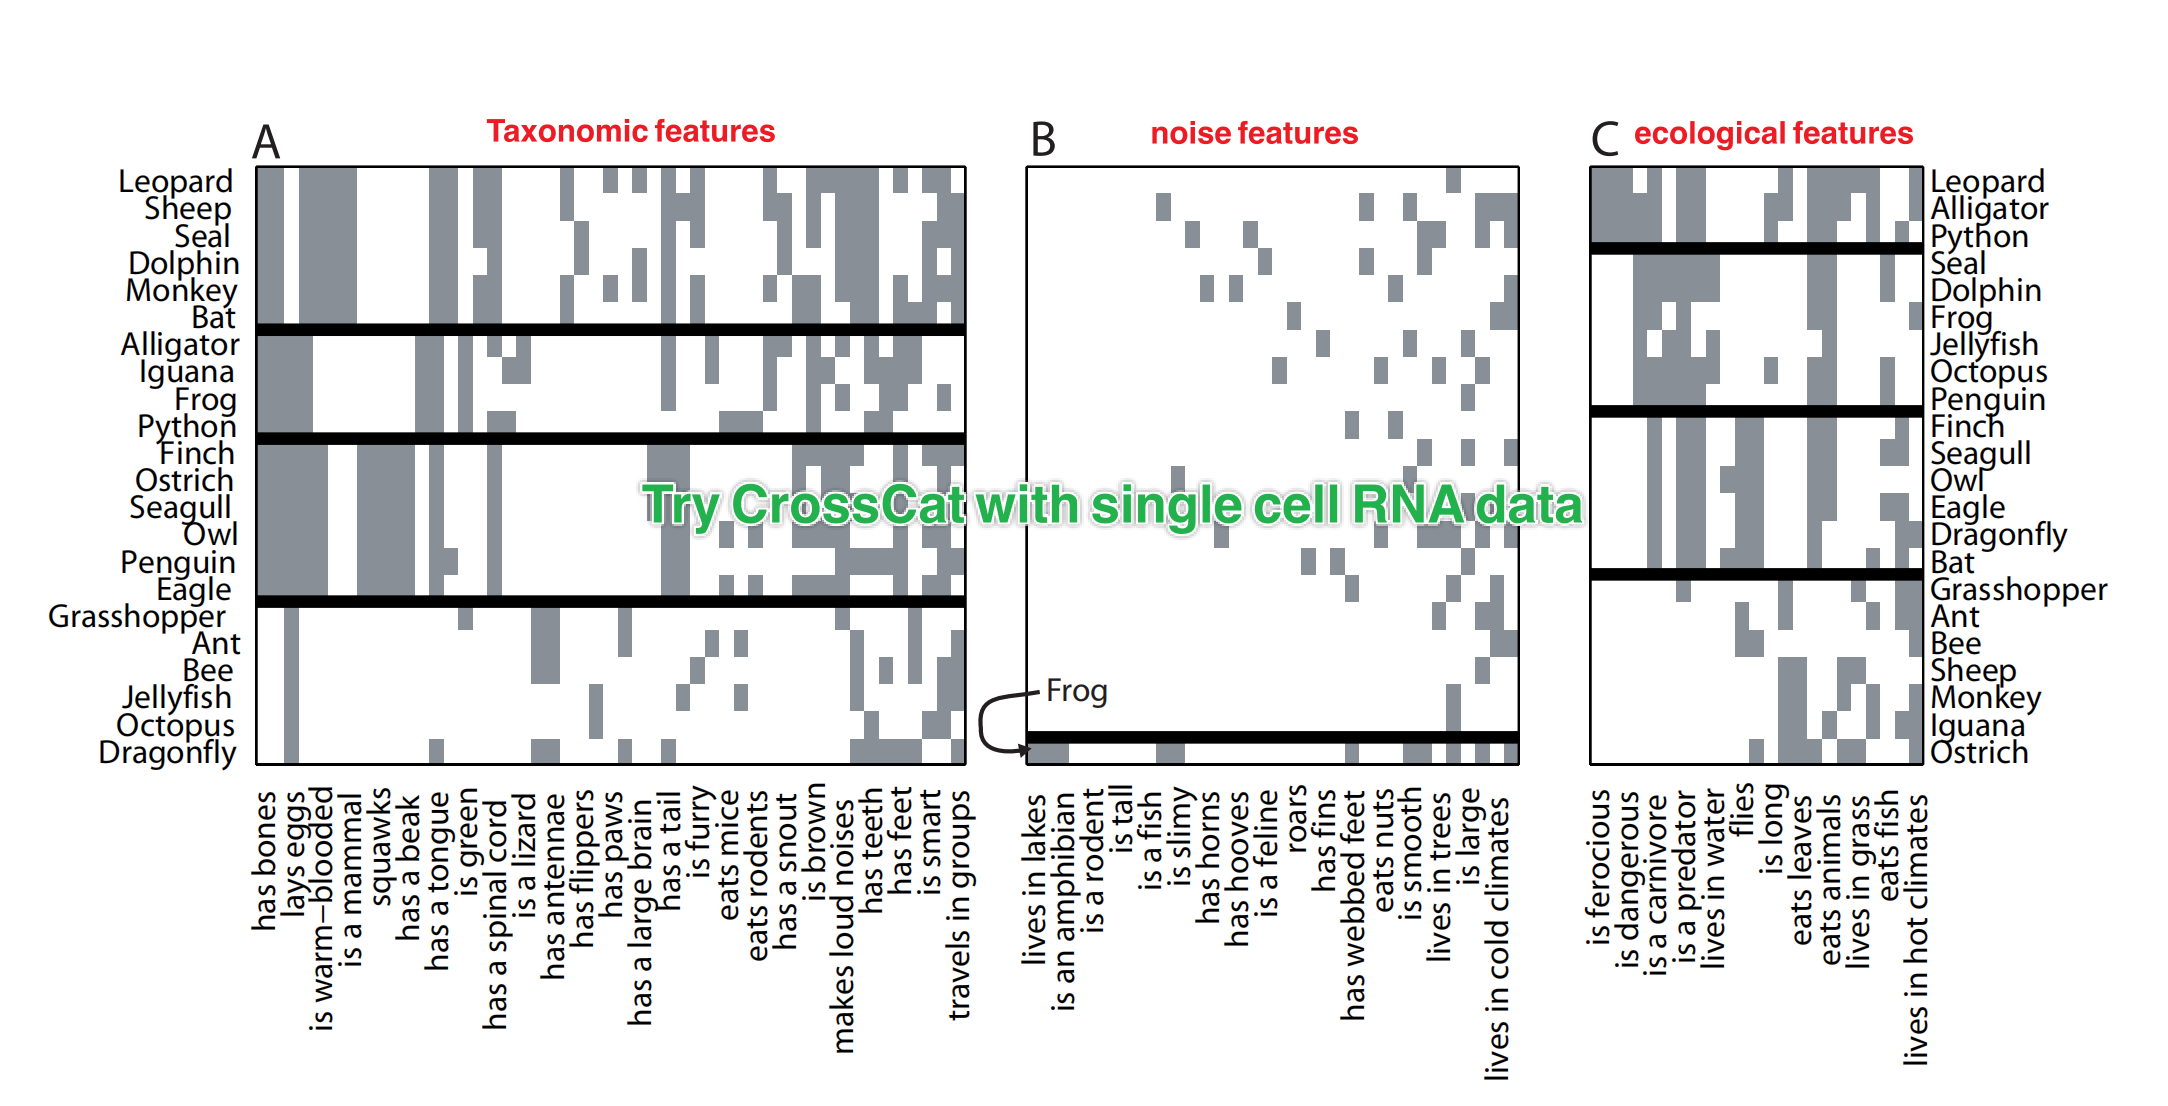
\includegraphics[width=\textwidth]{figs/crosscat.png}
    \caption{MAP estimate produced by the \textbf{CrossCat} system, \textbf{CrossCat}, nested partition models for biclustering.}
    \textit{It can be applied to scRNA data to discovery novel bi-label cell types}
    \label{fig:crosscat}
\end{figure}

\subsection{Graph Embeddings}

\begin{figure}[htpb]
    \centering
    \begin{tikzpicture}[
        datanode/.style={rectangle, solid, draw=black!85, rounded corners=.1cm, fill=orange!15, minimum size=10mm},
        networknode/.style={rectangle, solid, draw=black!85, rounded corners=.1cm, fill=violet!15, minimum size=10mm},
        lossnode/.style={rectangle, solid, draw=black!85, minimum size=10mm},
        dashedouter/.style={rectangle, draw=black!50, dashed, very thick, inner sep=5pt, inner xsep=2mm, inner ysep=3mm},
        dottedouter/.style={rectangle, draw=black!50, dotted, very thick, rounded corners=.2cm},
        ->,>=stealth',auto,node distance=7mm,thick]
        \tikzstyle{every node}=[font=\small,scale=0.9]

        \node[networknode] (enc) {$\mathrm{ENC}(\mathbf{W},\mathbf{X};\mathbf{\Theta}^E)$};

        % \node[dashedouter, label=above:{Input}] (input) {
        % \begin{tikzpicture}[remember picture]
            \node[datanode, left = of enc] (X) {$\mathbf{X}$};
            \node[datanode, below = of X] (W) {$\mathbf{W}$};
        % \end{tikzpicture}
        % };

        \node[fit={(X) (W)}, dashedouter, label=above:{Input}, inner xsep=2mm, inner ysep=3mm] (output) {};
        
        \node[datanode, right = of enc] (Z) {$\mathbf{Z}$};
        \node[networknode, right = of Z] (decs) {$\mathrm{DEC}(\mathbf{Z};\mathbf{\Theta}^S)$};
        \node[networknode, below = of decs] (decd) {$\mathrm{DEC}(\mathbf{Z};\mathbf{\Theta}^D)$};

        % \node[dashedouter, label=above:{Output}] (output) {
        % \begin{tikzpicture}[remember picture]
            \node[datanode, right = of decs] (haty) {$\hat{\bm{y}}^S$};
            \node[datanode, below = of haty] (hatW) {$\hat{\mathbf{W}}$};
        % \end{tikzpicture}
        % };
        
        \node[fit={(haty) (hatW)}, dashedouter, label=above:{Output}] (output) {};
        
        \node[lossnode, right = of haty] (ls) {$\mathcal{L}_\text{sup}^S$};
        \node[lossnode, below = of ls] (lr) {$\mathcal{L}_\text{rec}^G$};

        \node[datanode, right = of ls] (ys) {$\bm{y}^S$};
        % \node[datanode, right = of lr] (hatW) {$\mathbf{W}$};

        \node[fit={(X) (W) (enc) (Z)}, dottedouter, draw=NavyBlue!40, inner xsep=6mm, inner ysep=4mm, ultra thick] (graphencnet) {};
        \node[anchor=south] at ([yshift=0.1cm]graphencnet.north) {\color{NavyBlue}\makecell{\textbf{Graph encoder network}: \\ graph structure + optional node features \\ $\to$ node embeddings}};

        \node[fit={(W) (decd) (hatW) (lr)}, dottedouter, draw=ForestGreen!40, inner xsep=11mm, inner ysep=4mm, ultra thick] (graphdecdnet) {};
        \node[anchor=north] at ([yshift=-0.1cm]graphdecdnet.south) {\color{ForestGreen}\makecell{\textbf{Graph decoder network}: \\ node embeddings $\to$ similarity scores}};

        \node[fit={(Z) (decs) (haty) (ls) (ys)}, dottedouter, draw=Maroon!40, inner xsep=8mm, inner ysep=3mm, ultra thick] (graphdecsnet) {};
        \node[anchor=south] at ([yshift=0.2cm]graphdecsnet.north) {\color{Maroon}\makecell{\textbf{Classification network}: \\ node embeddings $\to$ labels}};

        \node[fit={(Z)}, dottedouter, draw=ForestGreen!40, inner xsep=5mm, inner ysep=5mm, ultra thick] (graphdecdnet1) {};
        
        \draw[->] (X) -- (enc);
        \draw[->] (W) -| (enc);
        \draw[->] (enc) -- (Z);
        \draw[->] (Z) -- (decs);
        \draw[->] (Z) |- (decd);
        \draw[->] (decs) -- (haty);
        \draw[->] (decd) -- (hatW);
        \draw[->, dashed] (haty) -- (ls);
        \draw[->, dashed] (hatW) -- (lr);
        \draw[<-] (ls) -- (ys);
        \draw[->, dashed] (W) |- +(0,-1)-| (lr);
        % \draw[<-, dashed] (hatW) -- (W);
    \end{tikzpicture}
    \begin{gather}
        \mathcal{L} = \alpha \mathcal{L}^S_\text{sup}(\bm{y}^S,\hat{\bm{y}}^S;\mathbf{\Theta})
        + \beta \mathcal{L}_{\text{rec}}^G(\mathbf{W},\hat{\mathbf{W}};\mathbf{\Theta})
        + \gamma \mathcal{L}_\text{reg}(\mathbf{\Theta})
    \end{gather}
    where $S\in\{N,E,G\}$, $\mathbf{\Theta}=\{\mathbf{\Theta}^N,\mathbf{\Theta}^E,\mathbf{\Theta}^G,\mathbf{\Theta}^D\}$ and $\mathcal{L}_\text{reg}$ is regularization term.
    The overall loss is composed of supervised losses (optional), reconstruction loss, and regularization loss with weights.
    \caption{Framework of \textsc{GraphEDM}}
    \label{fig:graphedm}
\end{figure}


\begin{center}
    \textit{
    The remaining contents are organized like review without enough details.
    }
\end{center}










\newpage

\begin{framed}{\large
TODO list of the following week
\begin{itemize}
    \item start reading the sequent book without many notes;
    \item review and update the technologies for spatial transcriptomics;
    \item explore literature for research topics, including methodology and \textbf{biology}.
\end{itemize}
}
\end{framed}

\listnotes
\bibliography{ref}

\end{document}
